% FEUILLE DE STYLE
% CLASSE PRINCIPALE DU DOCUMENT
	\documentclass[a4paper,twoside,11pt,openany,fleqn]{book}
	% options: openright, openany
	
% BIBLIOGRAPHIE (A load avant frenchb/babel sinon warning)
	\usepackage[square,sort,semicolon]{natbib}
%	\usepackage[sectionbib]{chapterbib}
	\bibliographystyle{authordate1}
	\usepackage[nottoc]{tocbibind} %Pour que la biblio soit dans le sommaire

% PACKAGES BASIQUES
	\usepackage[english,frenchb]{babel} %Français
	\frenchbsetup{StandardLists = true}	% Remplace le tiret par un point dans les listes
	\usepackage[utf8]{inputenc} %UTF-8 (Accents)
	\usepackage{graphicx} %Ressources graphiques
	\usepackage[T1]{fontenc}
	
% CHAPITRES CUSTOM
	\usepackage[Rejne]{fncychap}
	% Options: Sonny, Lenny, Glenn, Conny, Rejne

% MARGES (Toujours avant fancyhdr)
	\usepackage[top=1in, bottom=1.25in, left=1in, right=1in]{geometry}

% EN-TÊTE ET PIED DE PAGE CUSTOM
	\usepackage{fancyhdr}
	\setlength{\headheight}{15pt}
	\pagestyle{fancy}
	
	% Define fancy styles
	\fancypagestyle{front}{%
		\fancyhf{} % Reset du fancy déjà existant
		\fancyfoot[RO]{\thepage} % Numéro de la page en bas à droite sur les pages paires
		\fancyfoot[LE]{\thepage} % Numéro de la page en bas à gauche sur les pages impaires
		\renewcommand{\headrulewidth}{0pt} % Ligne de tête
		\renewcommand{\footrulewidth}{0.5pt} % Ligne de pied
	}
	
	\fancypagestyle{front_light}{%
		\fancyhf{} % Reset du fancy déjà existant
		\fancyfoot[CO]{\thepage} % Numéro de la page au centre sur les pages paires
		\fancyfoot[CE]{\thepage} % Numéro de la page au centre sur les pages paires
		\renewcommand{\headrulewidth}{0pt} % Ligne de tête
		\renewcommand{\footrulewidth}{0pt} % Ligne de pied
	}
	
	\fancypagestyle{main}{%
		\fancyhf{} % Reset du fancy déjà existant
		\fancyhead[C]{\leftmark} % Nom du chapitre en haut au centre	
		\fancyfoot[RO]{\thepage} % Numéro de la page en bas à droite sur les pages paires
		\fancyfoot[LE]{\thepage} % Numéro de la page en bas à gauche sur les pages impaires
		\renewcommand{\headrulewidth}{0.5pt} % Ligne de tête
		\renewcommand{\footrulewidth}{0.5pt} % Ligne de pied
	}
	
	\fancypagestyle{star}{%
		\fancyhf{} % Reset du fancy déjà existant
		\fancyfoot[RO]{\thepage} % Numéro de la page en bas à droite sur les pages paires
		\fancyfoot[LE]{\thepage} % Numéro de la page en bas à gauche sur les pages impaires
		\renewcommand{\headrulewidth}{0.5pt} % Ligne de tête
		\renewcommand{\footrulewidth}{0.5pt} % Ligne de pied
	}
	
	\fancypagestyle{back}{%
		\fancyhf{} % Reset du fancy déjà existant
		\fancyfoot[RO]{\thepage} % Numéro de la page en bas à droite sur les pages paires
		\fancyfoot[LE]{\thepage} % Numéro de la page en bas à gauche sur les pages impaires
		\renewcommand{\headrulewidth}{0pt} % Ligne de tête
		\renewcommand{\footrulewidth}{0.5pt} % Ligne de pied
	}
	
	\fancypagestyle{part}{%
		\fancyhf{} % Reset du fancy déjà existant
		\fancyfoot[RO]{\thepage} % Numéro de la page en bas à droite sur les pages paires
		\fancyfoot[LE]{\thepage} % Numéro de la page en bas à gauche sur les pages impaires
		\renewcommand{\headrulewidth}{0pt} % Ligne de tête forcée invisible
		\renewcommand{\footrulewidth}{0pt} % Ligne de pied forcée invisible
	}

	% Redefine the plain page style
	\fancypagestyle{plain}{%
  		\fancyhf{}%
  		\fancyfoot[RO]{\thepage} % Numéro de la page en bas à droite sur les pages paires
		\fancyfoot[LE]{\thepage} % Numéro de la page en bas à gauche sur les pages impaires
		\renewcommand{\headrulewidth}{0pt} % Ligne de tête forcée invisible
		\renewcommand{\footrulewidth}{0.5pt} % Ligne de pied
  	}
  	
  	% Empty style on PART pages
  	\makeatletter
    \renewcommand\part{%
       \if@openright
         \cleardoublepage
       \else
         \clearpage
       \fi
       \thispagestyle{empty}%
       \if@twocolumn
         \onecolumn
         \@tempswatrue
       \else
         \@tempswafalse
       \fi
       \null\vfil
       \secdef\@part\@spart}
    \makeatother 
	
% TAILLE DES TITRES
	\usepackage{titlesec}
	\titleformat*{\section}{\LARGE\bfseries}
	\titleformat*{\subsection}{\Large\bfseries}
	\titleformat*{\subsubsection}{\large\bfseries}
	\titleformat*{\paragraph}{\large\bfseries}
	\titleformat*{\subparagraph}{\large\bfseries}

% ALPHANUM FOR APPENDIXES
	\usepackage{alphalph}
	
% PARAGRAPHE SPACING
	\setlength{\parskip}{\baselineskip}
	\setlength{\parindent}{0pt}
	
% ECRITURE MATHEMATIQUE
	\usepackage{amsmath}
	
% CONVERTION .eps VERS .pdf
	\usepackage{epstopdf}
	
% TABLEAUX
	{\renewcommand{\arraystretch}{1.5} %Taille des interlignes
	\usepackage{multirow}
	
% LISSAGE DE LA POLICE (Problème de hauteurs de certaines lettres)
	\renewcommand{\rmdefault}{pnc}
	\renewcommand{\sfdefault}{pag} 
	\renewcommand{\ttdefault}{pcr}
	
% LETTRINES
	\usepackage{lettrine}
	
% LIENS
	\usepackage{hyperref} %Liens dynamiques (Sommaire)
% Style dans le sommaire
	\hypersetup{
	    colorlinks,
	    citecolor=black,
	    filecolor=black,
	    linkcolor=black,
	    urlcolor=black
	}

% NUMEROTATION DES FOOTNOTES PAR PAGE
	\usepackage{perpage}
	\MakePerPage{footnote}
	
% INCLURE DES PDFs
	\usepackage{pdfpages}
	
% TABLE DES MATIERES PAR CHAPITRE
	%\usepackage{minitoc}
	%\setcounter{minitocdepth}{2}
	%\setlenght{\mtcindent}{24pt}
	%\renewcommand{\mtcfont}{\small\rm}
	%\renewcommand{\mtcSfont}{\small\bf}

% INDEX
	%\usepackage{imakeidx}
	%\makeindex[columns=2, title=Index, intoc]
	
% NOMENCLATURE
	%\usepackage{nomencl}
	%\makenomenclature[title=Nomemclature, intoc]
	
% RESET CHAPTER COUNTER FOR PARTS
	\makeatletter
	\@addtoreset{chapter}{part}
	\makeatother
	
% NUMEROTATION DES FIGURES/TABLES/EQUATIONS INDEP DU CHAPITRE
	\usepackage{chngcntr}
 
	\counterwithout{figure}{chapter}
	\counterwithout{table}{chapter}
	\counterwithout{equation}{chapter}

% BIBLIO AS PART
	\makeatletter
	\renewenvironment{thebibliography}[1]
     	{\part*{\bibname}
     	 \@mkboth{\MakeUppercase\bibname}{\MakeUppercase\bibname}%
    	  \list{\@biblabel{\@arabic\c@enumiv}}%
     	      {\settowidth\labelwidth{\@biblabel{#1}}%
        	    \leftmargin\labelwidth
            	\advance\leftmargin\labelsep
            	\@openbib@code
            	\usecounter{enumiv}%
            	\let\p@enumiv\@empty
            	\renewcommand\theenumiv{\@arabic\c@enumiv}}%
      	\sloppy
      	\clubpenalty4000
      	\@clubpenalty \clubpenalty
      	\widowpenalty4000%
      	\sfcode`\.\@m}
     	{\def\@noitemerr
       	{\@latex@warning{Empty `thebibliography' environment}}%
      	\endlist}
	\makeatother
	
% RENAME DES INSERTIONS AUTOMATIQUES (Laisser à la fin du fichier Style)
	\renewcommand{\listfigurename}{Liste des Figures}		%Figures
	\renewcommand{\listtablename}{Liste des Tables}			%Tables
	\renewcommand{\contentsname}{Sommaire}					%Sommaire
	\renewcommand{\bibname}{Références}						%Refs

% METADATA
\title{THÈSE DE DOCTORAT\\ \textbf{Immersion Visuelle Hyper-Réaliste et Multi-Sensorielle 3D}}
\author{}
\date{}

% DOCUMENT
\begin{document}
	
	% Page de garde	
	\frontmatter
	\maketitle

	% Préambule
	\pagestyle{front}
	\chapter*{Résumé}
\par La thèse <<~Immersion visuelle hyper-réaliste et multi-sensorielle 3D~>> a été réalisée dans le cadre d’un contrat CIFRE établit entre les Arts et Métiers d’une part et Renault SAS d’autre part. Elle propose un modèle de score permettant d’évaluer objectivement de la capacité d’un système d’affichage immersif à reproduire le bon niveau de stimulation sensorielle pour un utilisateur, par rapport à ce qu’il recevrait dans la réalité et à la modélisation du système visuel humain.

\par Dans un premier temps nous nous sommes intéressés à poser les bases du modèle : celui-ci est composé de douze critères, répartis équitablement en une somme d’indices de vision et d’indices d’immersion. Chaque critère se voit attribuer, dans la mesure du possible, une note de 0 à 100. La note de 0 représente l’incapacité du système visuel à percevoir ou à utiliser les informations visuelles, tandis que la note de 100 incarne la capacité maximale. Une note de 80 est également assignée pour la performance standard. Chaque critère se voit assigner une pondération en fonction de la tâche réalisée en environnement virtuel.

\par Nous réalisons dans un second temps une série d’expérimentations afin de compléter les informations disponibles dans la littérature, pour l’établissement des critères. On s’intéresse plus particulièrement au contraste et à la latence. La première expérimentation consiste en la transposition et la validation d’un modèle de performance visuelle en Réalité Virtuelle. Dans la seconde, on compare les effets de la latence sur une tâche donnée, entre un simulateur de type CAVE et un casque de Réalité Virtuelle.

\par La thèse propose un certain nombre de résultats tant théoriques et méthodologiques qu’expérimentaux. En condition d’immersion virtuelle, les critères de contraste et de luminance sont importants pour la perception visuelle. Les expériences réalisées montrent qu’un modèle adapté aux conditions d’immersion virtuelle est nécessaire. Par ailleurs, on montre que des seuils d’influence de la latence sur la performance semblent exister. On vérifie également la pertinence de corrélations entre performance, présence et mal du simulateur, en fonction de la latence et du système immersif.


\chapter*{Abstract}
\par The thesis "Hyperrealistic and multi-sensorial 3D visual immersion" was carried out within the framework of a CIFRE contract established between Arts et Métiers on the one hand and Renault SAS on the other. It proposes a score model to objectively evaluate the ability of an immersive display system to reproduce the right level of sensory stimulation for a user, compared to what he would receive in reality and to the modeling of the human visual system.

\par First, we were interested in laying the foundations of the model: it is composed of twelve criteria, equitably divided into a sum of vision indices and immersion indices. Each criterion is given, as far as possible, a score from 0 to 100. A score of 0 represents the visual system's inability to perceive or use visual information, while a score of 100 represents maximum capacity. A score of 80 is also assigned for standard performance. Each criterion is assigned a weight according to the task performed in the virtual environment.

\par We then carry out a series of experiments to complete the information available in the literature, to establish the criteria. Contrast and latency are of particular interest. The first experiment consists in the transposition and validation of a visual performance model in Virtual Reality. In the second, we compare the effects of latency on a given task, between a CAVE simulator and a HMD.

\par The thesis proposes a number of theoretical, methodological and experimental results. In virtual immersion conditions, contrast and luminance criteria are important for visual perception. Experiments show that a model adapted to virtual immersion conditions is necessary. Furthermore, we show that thresholds of latency influence on performance seem to exist. The relevance of correlations between simulator performance, presence and cyber-sickness is also checked, depending on the latency and the immersive system.

\chapter*{Remerciements}
\par Tarifs pour apparaitre dans les remerciements:
\begin{itemize}
	\item Citation générale dans un groupe: gratuit.
	\item Citation nominale: 5 euros.
	\item Paragraphe personnel: 15 euros.
	\item Photo personnelle avec des cœurs: 106 euros.
\end{itemize}

	\tableofcontents					% Sommaire
	\listoffigures						% Figures
	\listoftables						% Tables
	
	% Introduction générale
	\mainmatter
	\chapter*{Introduction générale}
\addcontentsline{toc}{part}{Introduction générale}
\markboth{INTRODUCTION GÉNÉRALE}{}

\lettrine[lines=3]{L}{orem} ipsum dolor sit amet, consectetur adipiscing elit. Proin quis ipsum tellus. Cras placerat nulla sit amet urna iaculis sagittis. Curabitur ullamcorper leo est, at tempor nunc malesuada vitae. Sed ullamcorper tempus vehicula. Integer sit amet nulla ac lectus vulputate bibendum sed in arcu. Suspendisse potenti. Sed dapibus velit quis auctor pretium. Ut dictum, nisl ut tincidunt aliquam, odio orci dignissim libero, eu maximus dolor justo ut lorem. Duis accumsan sed dolor id elementum. Maecenas erat turpis, tincidunt quis sem vestibulum, tempor sagittis turpis. Vestibulum luctus congue nisl, non porttitor felis. Pellentesque eget nisl et nisl fringilla efficitur sed id nibh. Maecenas volutpat dolor ac lorem iaculis ultricies.

\par Nulla consectetur elit ac ante aliquam condimentum. Donec eu auctor turpis. Quisque purus ligula, viverra ut luctus quis, ultricies ac leo. Pellentesque habitant morbi tristique senectus et netus et malesuada fames ac turpis egestas. Nam vel est enim. Suspendisse elementum fermentum blandit. Curabitur volutpat et turpis in condimentum. Proin dignissim nec nisl sit amet accumsan. Ut facilisis nulla at mi porttitor, nec venenatis mi pretium. Proin interdum aliquam odio, quis convallis nunc lobortis eget.
	
	% Chapitres
	\pagestyle{main}
	\part{État de l'Art: Partie Théorique}
\label{part:edla}

\chapter{Définition du réalisme}
\label{chap:def_realisme}
	\section{Enjeux et problématique}
	\par Qu'est-ce que le réalisme ? Comment le définir ? A quoi peut-il servir ? Peut-on faire <<~plus~>> de réalisme ? A quoi cela servirait-il ? Ces questions peuvent devenir des enjeux majeurs lorsqu'elles sont associées à des cas d'application réels et de portée économique importante. Un exemple flagrant se retrouve à l'endroit du constructeur français de voitures: Renault.
		
	\par Les maquettes et prototypes numériques entrent de plus en plus dans le cycle de conception des véhicules. Les simulateurs et autres systèmes d'affichage immersif sont utilisés pour visualiser ces maquettes à l'échelle 1:1, dans des conditions d'utilisation, d'illumination et de ressemblance poussées à leur paroxysme. L'objectif est d'être le plus <<~réaliste~>> possible afin de légitimer au maximum la prise de décisions dans les simulateurs.
	
	\par Mais définir -et plus encore, quantifier- le \textit{réalisme} n'est pas une tâche facile. Nous allons voir qu'il peut exister, voire coexister, plusieurs définitions applicatives du concept.
	
	\section{Définitions usuelles}
	\par Une fois l'évidence de la recherche de réalisme mise en avant, il devient nécessaire de définir ce qu'est le réalisme, sans quoi il serait impossible de le travailler. Tout d'abord, on peut s'intéresser à la définition que donne le Larousse \footnote{Réalisme. (s.d.). Dans \textit{Dictionnaire Larousse en ligne}. Repéré à \url{www.larousse.fr/encyclopedie/divers/réalisme/8600}}:
	\begin{itemize}
		\item Attitude qui tient compte de la réalité telle qu'elle est.
		\item Caractère de ce qui est une description objective de la réalité, qui ne masque rien de ses aspects les plus crus.
		\item Tendance littéraire et artistique du XIXe siècle qui privilégie la représentation exacte, tels qu'ils sont, de la nature, des hommes, de la société.
		\item Doctrine qui affirme que la connaissance du réel constitue le réel lui-même, que cette connaissance soit la seule réalité ou qu'à côté d'elle figure une autre réalité, l'objet auquel elle s'applique.
	\end{itemize}
	
	\par Mais ces définitions (notamment les n.3 et 4) semblent assez peu utiles pour notre application car trop généraliste. Il faut s'intéresser à une définition qui soit spécifique au cadre de la réalité virtuelle (RV). Mais le <<~réalisme~>> en RV est un terme très ambivalent et difficile à cerner \citep{burkhardt_realite_2003}. C'est ce que nous allons étudier dans la prochaine sous-partie.
	
	\section{Définitions dans le domaine de la Réalité Virtuelle}	
	\par La première définition qui vient à l'esprit est celle de la ressemblance graphique avec le monde réel \citep{ferwerda_model_1996}. Est réaliste ce qui semble vrai ou beau, ce qui donne l'impression d'être vrai. On s'autorise alors l'utilisation d'un certain nombre d'artefacts graphiques (souvent issus de et popularisés par le cinéma), tel les bokehs\footnote{Les bokehs (terme provenant du japonais pour flou) sont des artefacts graphiques ressemblant à des taches de flou et qui prennent la forme du diaphragme de l'objectif de l'appareil de capture (caméra ou appareil photo)} (voir Fig. \ref{fig:bokeh_illustration}) ou le tonemapping (voir plus bas), afin de renforcer le sentiment d'apparence réelle. Ce type de réalisme est notamment développé par et mis en avant dans le monde du jeu vidéo avec des textures de plus en plus sophistiquées, des modélisations de plus en plus fines (et donc lourdes en polygones) mais surtout des jeux de lumière et d'optique saisissants.
	
	\begin{figure}
		\centering
		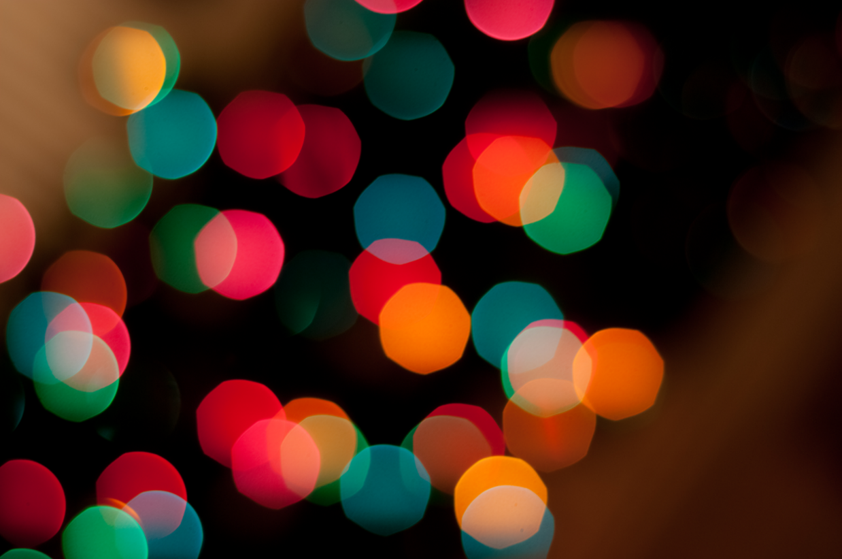
\includegraphics[scale=.75]{Figures/BokehIllustration}
		\caption{Illustration de bokeh}
		\label{fig:bokeh_illustration}
	\end{figure}
	
	\par Une deuxième approche, moins évidente au premier abord, est décrite chez Hoorn \citep{hoorn_virtual_2003}: un environnement virtuel sera jugé assez réaliste s'il remplit sa fonction ; si, dans le cadre d'une application d'apprentissage par exemple, ce qui doit être appris est appris, et si cet apprentissage en RV est transféré en-dehors du monde immersif. Cette définition se détache complètement d'une volonté d'un réalisme d'apparence (comme on a pu voir précédemment) et peut même se détacher d'une construction logique et/ou anthropomorphe de l'environnement virtuel. Si une scène faite de volumes géométriques colorés flottants dans un espace monochrome suffit à transmettre le message voulu, la scène est jugée réaliste.
	
	\par On trouve, dans \citep{fuchs_traite_2003}, une définition plus complète, divisée en cinq acceptations du terme \textit{réalisme} dans le domaine de la RV. Ces acceptations ne sont pas mutuellement exclusives mais il peut être nécessaire d'utiliser plusieurs d'entre elles pour construire sa définition du réalisme:
	\begin{itemize}
		\item Évaluation subjective du degré de ressemblance d'une situation.
		\item Fidélité de construction de la simulation aux lois de la Nature.
		\item Évaluation subjective du degré de crédibilité d'une situation.
		\item Fidélité psychologique.
		\item Illusion du réel (connue aussi sous l'appellation \textit{présence}).
	\end{itemize}
	
	\par La première acceptation, l'évaluation subjective du degré de ressemblance, a déjà été décrite dans un paragraphe précédent. Elle recouvre toute la partie esthétique et artistique de la conception de l'environnement virtuel.
	
	\par La deuxième acceptation, la fidélité de la simulation aux lois de la Nature, accorde moins d'importance à la beauté de la simulation qu'à son comportement simulé ; en dépit de ce que peut juger l'utilisateur. Chaque fonctionnalité implémentée se comporte en suivant un modèle issu du monde physique réel. De par le biais de perception qui peut être induit dans un monde virtuel, les comportements (comme par exemple la gravité, l'adhérence sur un sol, etc ...) et/ou les apparences (rendu des couleurs, floutage des images en fonction de la vitesse, ...) peuvent apparaitre comme non naturels à l'utilisateur. Son avis n'est pas pris en compte, on se contente d'afficher des modèles rigoureux.
	
	\par La troisième acceptation, est la création d'une expérience perceptive qui serait crédible du point de vue du système sensoriel, tant sur le plan microscopique (chaque élément pris à part) que sur le plan macroscopique (l'environnement virtuel dans sa globalité). Même si les informations qui sont envoyées à l'utilisateur (via l'interface de l'environnement virtuel) ne suivent pas rigoureusement les lois de la physique et du monde \textit{réel}, il faut que l'observateur les perçoive comme étant vraies.
	
	\par On peut supposer un lien fort et systématique entre cette dernière acceptation (perception crédible) et la précédente (construction objective via des modèles déterminés) mais cette question est encore grande ouverte et sujette à recherche.
	
	\par Ensuite, la quatrième acceptation du terme \textit{réalisme} est liée à une fidélité d'ordre psychologique. L'utilisateur doit se comporter de la même manière dans l'environnement virtuel que dans la même situation dans le monde physique. Les images affichées peuvent ne pas correspondre avec ce que l'utilisateur verrait dans la situation réelle (en fonction de la tâche à réaliser) tant que les performances et les résultats du sujet dans l'environnement virtuel sont similaires ou identiques à celles/ceux enregistré(e)s dans le monde réel. Cette acceptation est largement détaillée dans la littérature \citep{patrick_training:_1992,stoffregen_one_2003,burkhardt_realite_2003}.
	
	\par Enfin, la cinquième et dernière acceptation fusionne les concepts de \textit{réalisme} et de \textit{présence}. Plus le sentiment de présence dans un environnement virtuel sera fort, plus le réalisme dudit environnement le sera aussi. La présence est <<~l'illusion d'une réalité qui n'existe pas~>> \citep{stoffregen_one_2003}, c'est à dire le fait de faire croire au cerveau que les images/objets/personnes virtuelles que l'on voit sont en fait bien réels ou vivants \citep{burkhardt_realite_2003}. Plus la croyance en la réalité de la scène est forte, plus la présence est forte.
	
	\begin{figure}
		\centering
		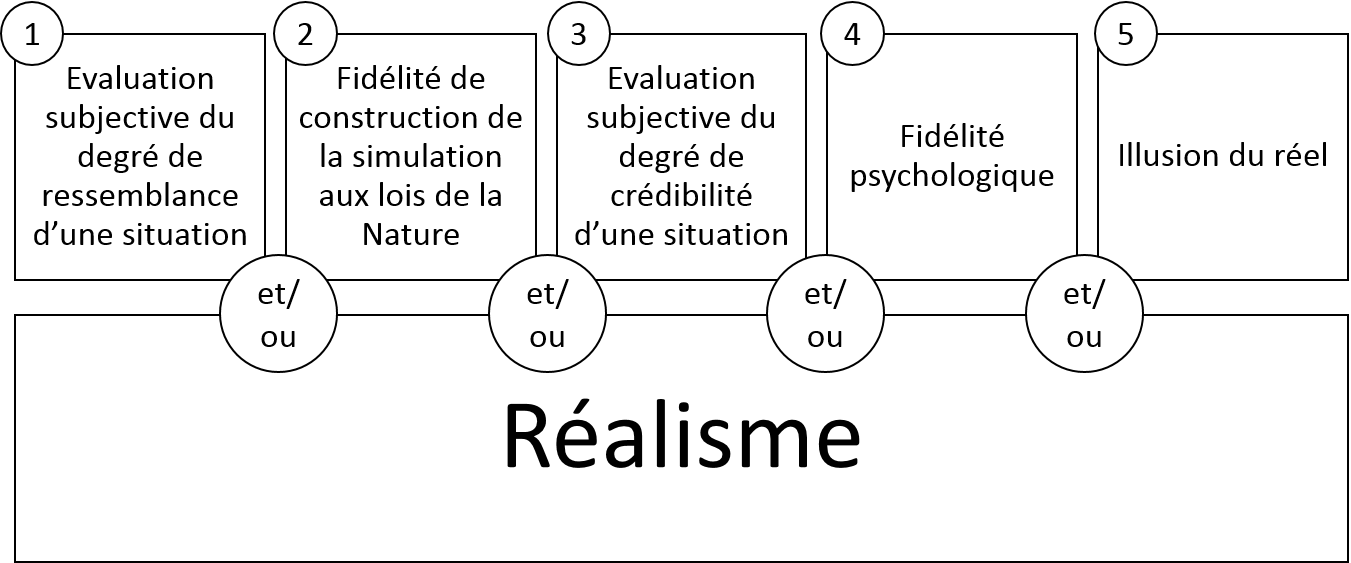
\includegraphics[scale=.65]{Figures/AcceptationsRealisme}
		\caption{Différentes acceptations du terme \textit{réalisme} chez \citep{fuchs_traite_2003}}
		\label{fig:acceptations_realisme}
	\end{figure}
	
	\section{Définition de la multi-sensorialité 3D}
	\subsection{Immersion}
	\par Deux sémantiques coexistent: l'immersion est à la fois l'action d'immerger un utilisateur dans un environnement complètement virtuel via des images de synthèse ; mais c'est aussi l'effet (avéré ou non) qu'a cette immersion sur ce même utilisateur. De manière plus formelle, on peut dire que l'immersion est le <<~degré et [la] qualité, par l'interface [d'un] système, du contrôle des entrées sensorielles pour chaque modalité de perception et d'action~>> (depuis \citep{fuchs_traite_2003}).
	
	\par Pour \cite{burkhardt_conception_1999}, le degré d'immersion est caractérisé par un ensemble de grandeurs:
	\begin{itemize}
		\item Le sous ensemble des modalités mises en œuvre dans l'interaction.
		\item Les propriétés des dispositifs d'interaction pour chacune des modalités visées (degré de complétude, qualité, paramètres du signal, ...)
		\item La cohérence interne et la latence globale de l'information et des réactions délivrées en temps réel par le système.
		\item Les propriétés physiques de l'environnement physique dans lequel se déroule l'expérience.
	\end{itemize}
	
	\subsection{Présence}
	\par Le concept de présence rassemble à la fois le(s) résultat(s) et l'effet d'une (bonne) immersion. Comme décrit dans \citep{burkhardt_realite_2003}: <<~[la présence] désigne l'effet de faire percevoir comme réels ou vivant, les objets, évènements ou personnages avec lequel l'utilisateur interagit dans l'environnement virtuel~>>.
	
	\section{Cadre d'étude}
	\par Dans notre cas, la définition du réalisme qui aura été retenue -et qui sera sous-entendue quand on utilisera le mot \textit{réalisme} seul- est celle de la proximité physiologique avec le système visuel humain.
	
	\par Le but de cette thèse n'est pas de construire de nouveaux modèles esthétiques et de travailler à l'amélioration graphiques des simulateurs (objectif qui incombe plutôt à un designer ou à un graphiste), ni d'élaborer un nouveau modèle de vision mais plutôt de travailler avec des modèles de vision, c'est à dire la manière dont la caméra virtuelle va extraire les informations de la scène virtuelle -par opposition aux modèles d'affichage qui décrivent comment les informations capturées par la caméras doivent être affichées sur le(s) écran(s)- pour déterminer des caractéritiques qui soient proches des facultés de la vision humaine.
	
	\begin{figure}
		\centering
		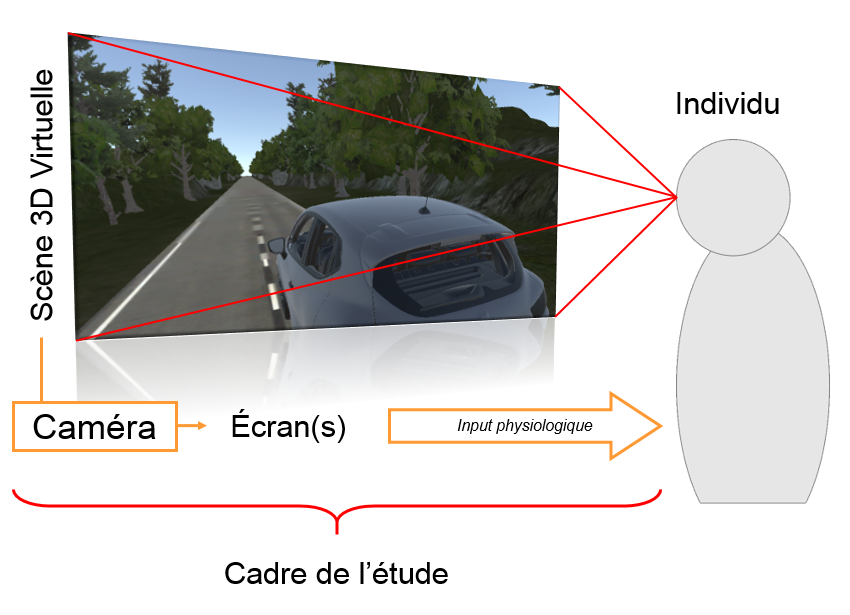
\includegraphics[scale=.65]{Figures/CadreEtude}
		\caption{Cadre d'étude de la thèse}
		\label{fig:champ_d_etude_these}
	\end{figure}
	
	\par Nos travaux dépassent le simple cadre du réalisme en tenant que tel de part leur implication dans le domaine de la Réalité Virtuelle: par construction, celle-ci met en jeu tous les sens de l'homme. \citep{burdea_realite_1993} résument bien en disant que <<~de part sa nature même, c'est à dire de par ses caractéristiques d'immersion et d'interactivité, le système de RV implique "presque tout l'homme": tous ses sens, toute son attention~>>.
	
	\par Dans le cadre de la thèse, le sens de <<~multi-sensorialité~>> n'est donc pas l'usage des plusieurs des cinq sens traditionnels (ouïe, vue, odorat, toucher et goût) mais plutôt la prise en compte de la temporalité de l'expérience et de la capacité de l'observateur de bouger dans son environnement, au bénéfice de la vision. Par exemple, la parallaxe de mouvement. Cela nous permettra d'englober les concepts de présence et d'immersion dans la réflexion autour de la thèse, avec ses impératifs de cohérence et de qualité de l'expérience utilisateur que cela implique.
	
	\par Le réalisme physiologique doit, par construction et par définition, se baser sur le système visuel humain. Dans la suite de ce chapitre, nous passerons en revue un grand nombre de paradigme de la vision afin d'établir précisément la compréhension de son fonctionnement.

\chapter{Fonctionnement de la vision}
\par Première interface et premier organe de la chaine, l'œil -à contrario de ce qui est généralement pensé- n'est pas la pièce maitresse de la vision: il ne sert \textit{qu'à} envoyer des signaux électriques au cerveau et pourrait être remplacé par une caméra par exemple, dans la mesure où celle-ci émet les bonnes informations à travers le nerf optique \citep{dobelle_artificial_2000}. L'œil reste néanmoins un outil très puissant et versatile. Nous allons ici rappeler le fonctionnement de l'œil et de la vision, qui se traduit par les informations collectées et transmises par l'œil puis traitées par le cerveau. Le sujet est tout à fait connu et largement documenté \citep{fairchild_human_2005,wandell_foundations_1995,gross_human_2008,driscoll_eyes_1978}.

	\section{Structure de l'œil}
	\par L'œil se divise en un certain nombre de parties dont les principales sont la cornée, l'iris, la pupille, le cristallin, la rétine et les deux chambres contenant les humeurs aqueuse et vitrée. Toute la structure de l'œil est résumée sur la Fig. \ref{fig:oeil}.
	
	\par La cornée est la première interface entre l'extérieur et l'intérieur de l'œil.
	
	\par Le cristallin est la lentille principale de l'œil et va s'occuper de la netteté du monde qui nous entoure via le processus d'accommodation. Le principe est simple: il faut placer le foyer image de l'œil sur la rétine (voir Section suivante). Pour ce faire, l'œil accommode, c'est à dire qu'il va modifier sa géométrie dans le but de modifier ses propriétés optiques. Dans la pratique, les muscles ciliaires font se déformer le cristallin (voir Fig. \ref{fig:oeil}) en réduisant sa hauteur et donc en augmentant sa convexité ou inversement. Ce processus dure 1 seconde et n'est pas définitif: une fois l'œil accommodé, celui-ci oscille légèrement autour de la valeur  d'accommodation, à une fréquence de 5 Hz. Ce mécanisme permet de récupérer des feedbacks en cas d'ajustements à opérer \citep{gross_human_2008}.
	
	\par Le mécanisme d'accommodation ne fonctionne plus à partir d'un certain seuil de luminosité. Ce seuil est évalué à $0.01~cd/m^2$. En l'absence d'accommodation, l'œil prend une position intermédiaire entre la position relâchée (accommodation à l'infini) et une position \textit{presque-accommodée} \citep{gross_human_2008}.
	
	\par Ensuite, la pupille et l'iris sont intimement liées car la première est l'espace laissé par la seconde au centre de l'œil. L'iris est une composante contrôlable de l'œil. L'iris contrôle la quantité de lumière qui arrive dans l'œil et donc sur la rétine. Plus la pupille sera grande, plus la lumière pourra rentrer dans l'œil. Un œil humain peut supporter des luminosité (luminance) allant de $10^-6$ à $10^5~cd/m^2$. La variation du diamètre de la pupille peut être modélisé par une modèle mathématique. Si il en existe un certain nombre dans la littérature (voir \citep{watson_unified_2012} pour un état de l'Art exhaustif) on donne ici l'équation suivante (Eq. \ref{eq:diam_pupille}). De la même manière que l'accommodation, le diamètre de la pupille oscille autour de sa valeur moyenne à l'instant t. Ce phénomène est appelé \textit{hippus} \citep{gross_human_2008}.
	
	\begin{equation}
		log_{10}(D_{iris}) = 0.8558 - 0.000401 \cdot [8.4 + log_{10}(L)]^3
		\label{eq:diam_pupille}
	\end{equation}
	
	\par De la même manière, la vergence est la capacité des yeux de s'orienter vers le point d'accommodation lorsque celui est proche. On appelle convergence le phénomène qui consiste à augmenter l'angle formé par l'intersection des lignes du regard de chaque œil (quand la cible se rapproche) et divergence le cas inverse, lorsque cet angle diminue (la cible s'éloigne). Le processus possède une latence estimée à 150 ms et une durée approximative évaluée à 0.2 - 0.6 secondes \citep{devisme_optimisation_2004, gross_human_2008}.
	
	\par L'œil humain a une taille globalement constante entre les individus: autour de 24 mm de diamètre \citep{glassner_principles_1995}. Le pouvoir optique de l'œil, c'est à dire sa capacité à adapter ses propriétés optiques, se mesure en dioptries. Les dioptries ($\delta$) sont l'inverse de la distance focale d'un système optique, elles sont homogènes à des $m^{-1}$. Faire varier ses dioptries (et donc sa distance focale) permet l'accommodation et l'adaptation de l'œil. L'œil humain possède environ 42$\delta$ en fonctionnement et peut monter jusqu'à une puissance de 60 à 80$\delta$ pour compenser les défauts de l'œil \citep{glassner_principles_1995}.
	
	\par La rétine tapisse le fond de l'œil et est composée de millions de récepteurs photosensibles qui vont être responsable de la captation de l'image. Ces photo-récepteurs sont les cônes, sensibles à la couleur, et les bâtonnets sensibles à la luminosité. Il existe 3 types de cônes, qui sont chacun sensibles à différentes longueurs d'onde: on retrouve les cônes de type S (pour \textit{small}, petite longueur d'onde) avec un maximum de sensibilité à $420~nm$ ; ensuite, on trouve les cônes de type M (pour \textit{medium}, moyenne longueur d'onde) avec un maximum de sensibilité à $530~nm$ ; et enfin, on a les cônes de type L (pour \textit{long}, grande longueur d'onde) avec un maximum de sensibilité à $560~nm$. Le seul message émanant d'un cône ou d'un bâtonnet est celui de son activation. La reconnaissance des couleurs et de l'intensité de la lumière se fait par la combinaison des résultats d'activation des différents types de cône ; ce procédé est analogue à celui du tramage\footnote{Tramage: Procédé permettant de générer de nouvelles couleurs à partir d'une base limitée de couleurs. Typiquement, en informatique, les pixels des écrans sont en fait composés de 3 sous pixels: blanc, rouge et vert. Une fois combinés et vus d'assez loin, ils semblent ne créer qu'une seule couleur, potentiellement différente.} en informatique. Alors que l'on pourrait penser qu'il existe un cône dédié à chaque couleur, l'œil humain ne possède que trois types de cône. En effet, si l'œil possédait de nombreux autres types de cônes, la densité par cône serait grandement réduite et donc la finesse de vision avec \citep{glassner_principles_1995}.
	
	\par Les cônes et les bâtonnets ont chacun leur plage de fonctionnement optimale. Dans le domaine photopique (lumière du jour), les cônes sont saturés en luminosité et sont beaucoup moins efficaces que dans le domaine scotopique (de nuit). De leur côté, les cônes adaptent leur maximum de saturation par rapport au niveau global d'illumination \citep{glassner_principles_1995}.
	
	\par Enfin, la répartition des cônes et des bâtonnets sur la rétine n'est pas du tout homogène (voir Fig. \ref{fig:densite_cones_batonnets}). Une zone de la rétine présente une extrême concentration de cônes. Cette zone est appelée \textit{fovéa}. De par l'utilité des cônes et par construction du système optique de l'œil, c'est l'endroit où les rayons lumineux issus de la cible regardée convergent. On retrouve, en périphérie de la fovéa, les bâtonnets. Ce qui est capté par la fovéa est vu net, tandis que ce qui est capté par les bâtonnets ne l'est pas. L'axe de vision est d'ailleurs définit par le rayon issu du point nodal image jusqu'à la fovéa (voir section suivante). Cet axe, représenté sur la Fig. \ref{fig:modele_liou_brennan} est donc fixe et l'angle qu'il forme avec l'axe optique de l'oeil (ici appelé \textit{alpha}) vaut entre 3 et 8 degrés suivant les individus \citep{gross_human_2008}.
	
	\par La rétine n'est que la première étape du système d'acquisition et la totalité de celui-ci ainsi que le traitement par le cerveau sera traité plus loin dans le chapitre. D'abord, on se concentre sur la modélisation de l'œil.
	
	\begin{figure}
		\centering
		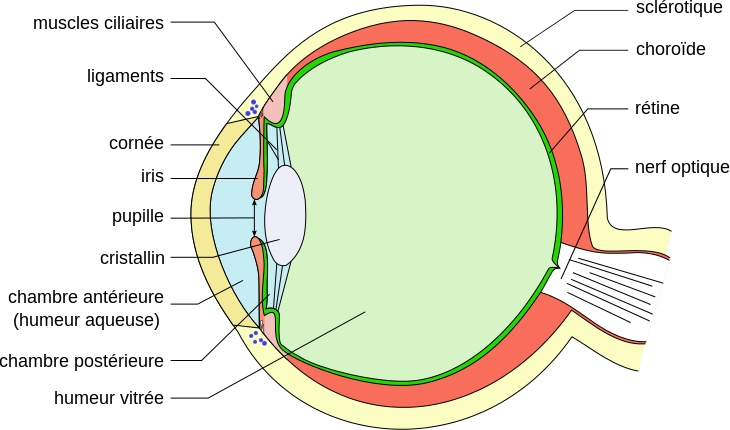
\includegraphics[scale=.4]{Figures/SchemaOeil}
		\caption{Structure de l'œil}
		\label{fig:oeil}
	\end{figure}
	
	\begin{figure}
		\centering
		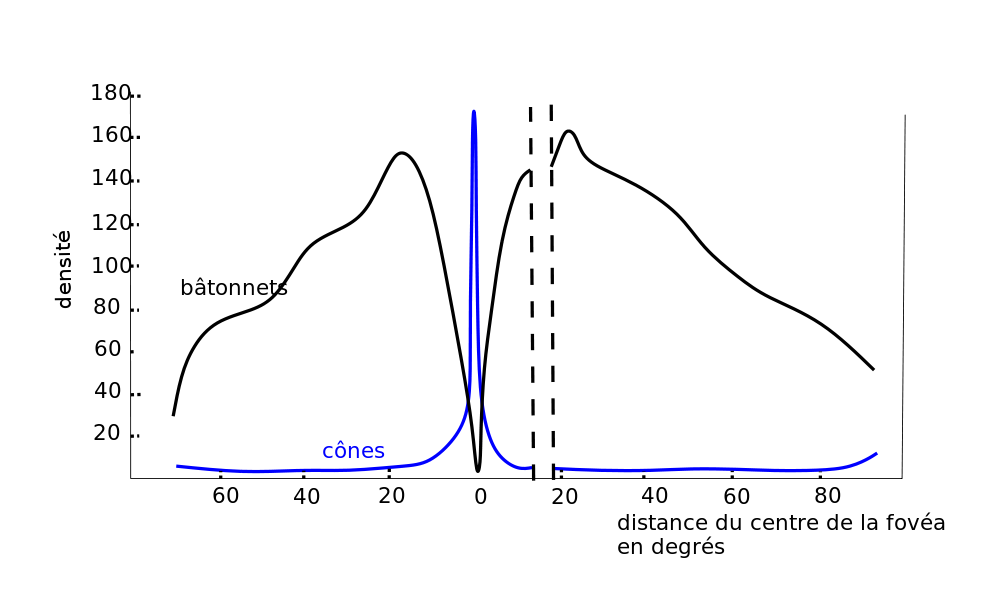
\includegraphics[scale=.35]{Figures/DensiteConesBatonnets}
		\caption{Répartition (en $milliers/mm^2$) des cônes/bâtonnets sur la rétine}
		\label{fig:densite_cones_batonnets}
	\end{figure}
	
	\section{Modélisation de l'œil}
	\par De nombreux scientifiques se sont intéressés à la compréhension et la modélisation de l'œil, et ce, dès la moitié du XIXe siècle avec Carl Friedrich Gauss qui en a définit les grands principes optiques. Cependant, avant de discuter des différents modèle de l'œil qui ont pu émerger au cours (notamment) du XXème siècle, il parait nécessaire de re-poser certaines bases élémentaires de l'optique géométrique.
	
	\par On note quelques points particulier dans un système optique simple (type lentille concave ou convexe). De manière générale, on rappelle que les points caractéristiques d'un lentille sont qualifiés d' \textit{objet} quand ils sont avant la lentille (en terme de trajet du rayon lumineux) et d' \textit{image} lorsqu'ils sont après la lentille. Par convention, un point caractéristique est noté avec une lettre majuscule tandis que son point conjugué image est noté avec la même lettre agrémentée d'un \textit{prime}.
	\begin{itemize}
		\item Le foyer objet est le point à partir duquel les rayons émergents sont ensuite dirigés vers l'infini optique (c'est à dire parallèle à l'axe optique) après passage par la lentille. Le foyer objet est noté F.
		\item Le foyer image est le point vers lequel convergent tous les rayons issus de l'infini avant la lentille. Dans le cas d'un œil sain (sans problèmes ophtalmologiques de type myopie ou hypermétropie), ce point doit être confondu avec la rétine pour avoir une image nette. Comme on a pu voir précédemment, c'est là le principal mécanisme de l'accommodation qui va déformer le système optique pour déplacer les foyers afin de faire la netteté sur la rétine. Le foyer image est noté F'.
		\item Le point central, par lequel un rayon passe sans être dévié, qui correspond au centre de rotation de l'œil. Il est noté C.
		\item Le point nodal objet est un point très particulier parce qu'il peut être considéré comme l'équivalent du \textit{point de vision}, c'est à dire le point où on pourrait ramener l'intégralité de l'œil à un équivalent ponctuel. Dans un système optique, il est défini comme le point par lequel passe un rayon lumineux avec une incidence donnée et ressort au point conjugué avec la même incidence. Il n'existe que dans un système optique complexe (fait de plusieurs lentilles ou interfaces optiques). Dans le cas d'une lentille simple seule il est confondu avec le centre. Ce point est globalement situé 6 mm à l'avant du centre de l'œil, sur l'axe optique \citep{gross_human_2008,ogle_optics:_1968}. Les points nodaux sont notés N et N'.
	\end{itemize}
	
	\begin{figure}
		\centering
		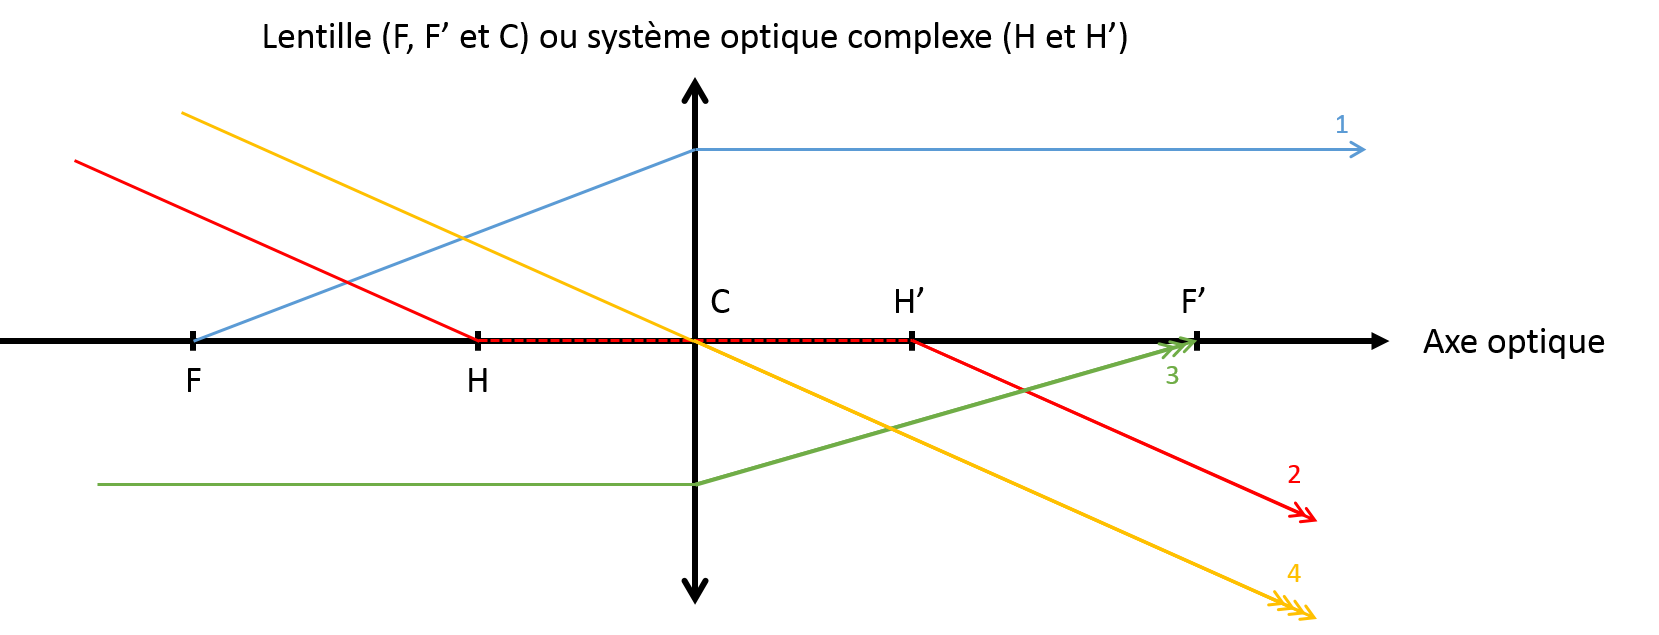
\includegraphics[scale=.5]{Figures/PointsSystemeOptique}
		\caption{Points caractéristiques (cardinaux) d'un système optique plan}
		\label{fig:points_cardinaux_systeme_optique}
	\end{figure}
	
	\par L'œil possède deux axes principaux: l'axe optique, qui passe par les centres de toutes les surfaces optiques ou composantes de l'œil (cristallin, pupille, ...) et l'axe de vision qui est composé en fait de deux demi-axes que sont les rayons qui passent par les points nodaux et jusqu'à la fovéa. L'œil est orienté selon l'axe optique mais la vision se fait le long de l'axe dit \textit{de vision}. La vision hors axe est appelée \textit{vision périphérique}.
	
	\par Enfin, un grand nombre de modèle de l'œil on été proposés, plus ou moins complexes, avec notamment des variations sur le nombre de surfaces optiques, jusqu'à l'adoption du modèle de \citep{liou_anatomically_1997}. Malgré tout ce modèle est tout sauf définitif et est toujours susceptible d'être amélioré ou affiné dans le futur. On présente une liste pas non-exhaustive des différents modèles de l'œil qui ont pu être élaborés au cours du XXème siècle \citep{liou_anatomically_1997,gross_human_2008}:
	\begin{itemize}
		\item Modèle de Helmholtz - Laurence (1909)
		\item Modèle de Gullstrand (1911): modèle le plus utilisé, notamment car un grand nombre de distances (taille de l'œil, distances focales, distance de la pupille, ...) et tous les indices de réfractions des différents milieux de l'œil y sont reportés (voir Fig. \ref{fig:modele_gullstrand}). Le modèle optique théorique pour la propagation de la lumière est composé de 3 surfaces.
		\item Modèle de Emsley (1946): modèle simplifié réduit à 1 seule surface.
		\item Modèle de Lotmar (1971): modélisation de la cornée et de la face arrière du cristallin par des surfaces polynomiales (plutôt que des sections de sphère).
		\item Modèle de Kooijman (1983): modèle en 4 surfaces, ajout d'asphéricités sur les surfaces sphériques.
		\item Modèle de Navarro (1985): idem que Kooijman avec des effets chromatique type dispersion de la lumière en plus.
		\item Modèle de Schwiegerling (1995)
		\item Modèle de Liou \& Brennan (1997): modèle à 5 surfaces dont 1 purement théorique (voir Fig. \ref{fig:modele_liou_brennan}). C'est la modèle le plus utilisé dans le domaine du calcul et de la simulation de rayons. 
	\end{itemize}
	
	\begin{figure}
		\centering
		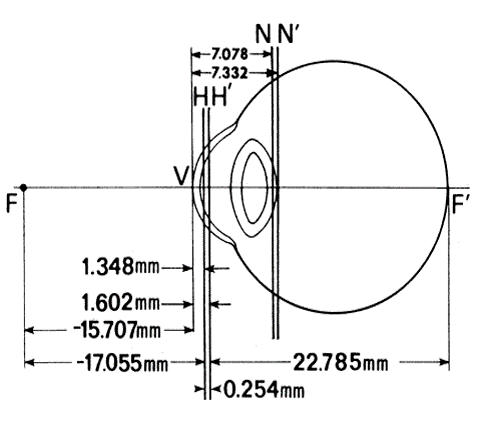
\includegraphics[scale=1.25]{Figures/GullstrandModel}
		\caption{Modèle et valeurs physiologiques de Gullstrand, image tirée de \citep{liou_anatomically_1997}}
		\label{fig:modele_gullstrand}
	\end{figure}
	
	\begin{figure}
		\centering
		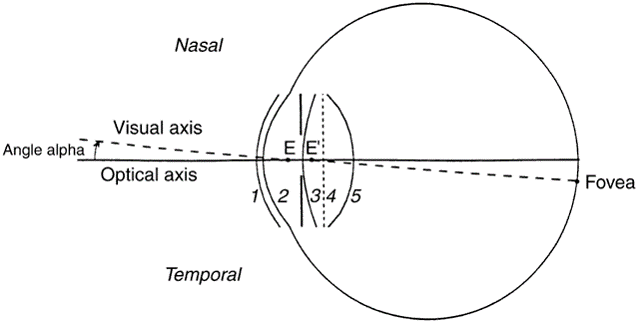
\includegraphics[scale=1]{Figures/LiouBrennanModel}
		\caption{Modèle de Liou \& Brennan, image tirée de \citep{liou_anatomically_1997}}
		\label{fig:modele_liou_brennan}
	\end{figure}
	
	\par Jusqu'à présent, nous avons détaillé le fonctionnement d'un œil seul. Nous allons maintenant nous intéresser à la vision binoculaire, c'est à dire de deux yeux en même temps.
	
	\section{Vision binoculaire}
	\par La vision binoculaire est avant tout un excellent outils de compréhension de l'environnement qui nous entoure, et notamment de la profondeur: le cerveau peut comparer en temps réel deux points de vue légèrement différents et en tirer des conclusions.
	
	\par L'élément de fonctionnement de la vision binoculaire est les disparités, c'est à dire la différence de position relative entre les deux images perçues (une par œil) d'un même objet. Si un objet est pleinement centré sur l'image perçue par l'œil gauche, il sera vu légèrement décalé du centre par l'œil droit.	Il existe deux types de disparités; les disparités verticales et les disparités horizontales \citep{devisme_optimisation_2004}.
	
	\par Les disparités horizontales sont générées par une différence angulaire sur le plan de l'azimut. Elles sont en charge de la perception relative de la distance, c'est à dire à la perception de la profondeur (relief).
	
	\par Les disparités verticales sont issues de la perception par les yeux d' une différence d'élévation pour le même point. Elles peuvent aussi apparaitre si un des yeux est plus proche de l'objet que l'autre (on parle alors de grossissement différentiel). Les disparités verticales permettent d'estimer la distance absolue d'un objet ainsi que l'excentricité d'une surface, indépendamment de son orientation.
	
	\par Les disparités peuvent être source de fatigues dans le système visuel humain. Ce problème a été adressé notamment en ajoutant du flou sur les disparités les plus grandes, en ajoutant un flou périphérique pour reproduire le flou rétinien et en proposant un modèle de caméras convergentes qui génère des disparités plus conformes à la réalité \citep{aurat_immersion_2016}.
	
	\par L' horoptère est le lieu des points de disparité horizontale nulle pour un point de fixation donné, c'est à dire, à un instant t donné, lorsqu'on regarde à un endroit donné, il existe une infinité de points pour lesquels aucun disparité n'est perçue: ils sont au même endroit sur l'image perçue par l'œil gauche et par celle perçue par l'œil droit. Théoriquement, le lieu de ces points est un cercle passant par le point de fixation et par le premier point nodal (point nodal objet, H) de chaque oeil; ce cercle s'appelle le Cercle de Vieth-Müller. Dans la pratique, le lieu de l'horoptère n'est pas tout à fait un cercle et présente une légère déviation, nommée Déviation de Hering-Hillebrand (voir Fig. \ref{fig:horoptere_panum}) \citep{neveu_impact_2012}.
	
	\par Si on prend en compte les disparités verticales, le lieu des points de disparité horizontale-verticale nulle devient un cylindre (Extension du Cercle de Vieth-Müller).
	
	\begin{figure}
		\centering
		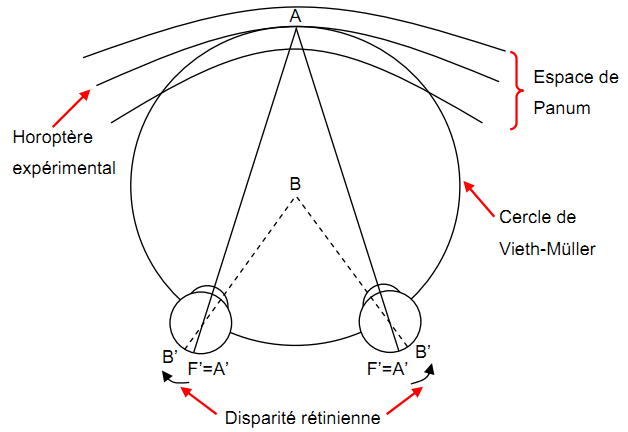
\includegraphics[scale=.55]{Figures/HoropterePanum}
		\caption{Horoptères théorique et empirique, Aire de Panum et disparités rétiniennes. Image tirée de \citep{neveu_impact_2012}.}
		\label{fig:horoptere_panum}
	\end{figure}
	
	\par L'œil possède une certaine capacité à adapter sa puissance (comme vu précédemment). On retrouve cette capacité au niveau du cerveau pour la fusion stéréoscopique. Dans une zone proche autour de l'horoptère (Aire de Panum) le cerveau écrase les disparités et fusionne quand même les images perçues par les yeux. L'étendue et la forme de l'aire de Panum est grandement dépendante des caractéristiques locales du stimulus \citep{devisme_optimisation_2004}.
	
	\par Enfin, la vision binoculaire est tributaire d'une certaine acuité stéréoscopique, c'est à dire la capacité à percevoir un écart de profondeur entre deux plans à une distance donnée. Celle ci est présentée et son modèle démontré à plusieurs endroits \citep{fuchs_traite_2003, gross_human_2008} et sera abordée dans un chapitre suivant. Toutefois, si l'âge et le niveau d'accommodation n'ont pas l'air d'affecter l'acuité stéréoscopique, cette dernière semble dépendante du contraste et de la quantité d'éclairement rétinien \citep{devisme_optimisation_2004}.
	
	\section{Traitement post-rétinien}
	\par Nous allons maintenant aborder toute la partie transmission et traitement par le cerveau du signal émis par les rétines. Le comportement précis dans le cerveau est encore à ce jour une question ouverte que nous traiterons donc dans les limites du possible et de l'utile dans le cadre de cette thèse. On ne peut ici que conseiller l'excellent \textit{Neurosciences: A la découverte du Cerveau} de \citep{bear_neurosciences:_2007}.
	
	\par Tout d'abord, il convient de développer quant à la structure même des cônes, de quelle manière ceux-ci jouent leur rôle de transducteur\footnote{Transducteur: Dispositif assurant une conversion ou un transfert de signaux et dans lequel un signal au moins est de nature électrique. (s.d.). Dans \textit{Dictionnaire Larousse en ligne}. Repéré à \url{http://www.larousse.fr/dictionnaires/francais/transducteur/79088}}: transformant un signal lumineux entrant en signal électrique sortant.
	
	\par La rétine est en fait composée de plusieurs types de cellules intermédiaires, les cônes et les bâtonnets n'étant qu'en bout de chaîne: cellules ganglionnaires, cellules amacrines, cellules horizontales et cellules bipolaires (voir Fig. \ref{fig:structure_retine}) \citep{bear_neurosciences:_2007}. Ces cellules se réunissent ensuite pour former le nerf optique et sortir de l'œil. Parmi les cellules ganglionnaires il en existe plusieurs types, chaque type véhiculant des informations différentes \citep{anses_effets_2014}.
	
	\par La voie magnocellulaire (M) représente 5\% de la population de cellules ganglionnaires. Ces cellules sont sensibles aux contrastes de luminance et ont une vitesse de conduction plutôt rapide. Elles sont à relier à la voie dorsale (voir plus loin).
	
	\par La voie parvocellulaire (P) représente 90\% de la population de cellules ganglionnaires. Ces cellules sont sensibles aux couleurs et, malgré une vitesse de conduction plus lente que les cellules de la voie M, elles répondent de manière tonique aux stimulations. Ces cellules sont à rapprocher de la voie ventrale.
	
	\par Enfin, il existe une voie M-non P qui représente les 5\% de population restants et participent à d'autres tâches que la vision pure (voir plus loin). 
	
	\begin{figure}
		\centering
		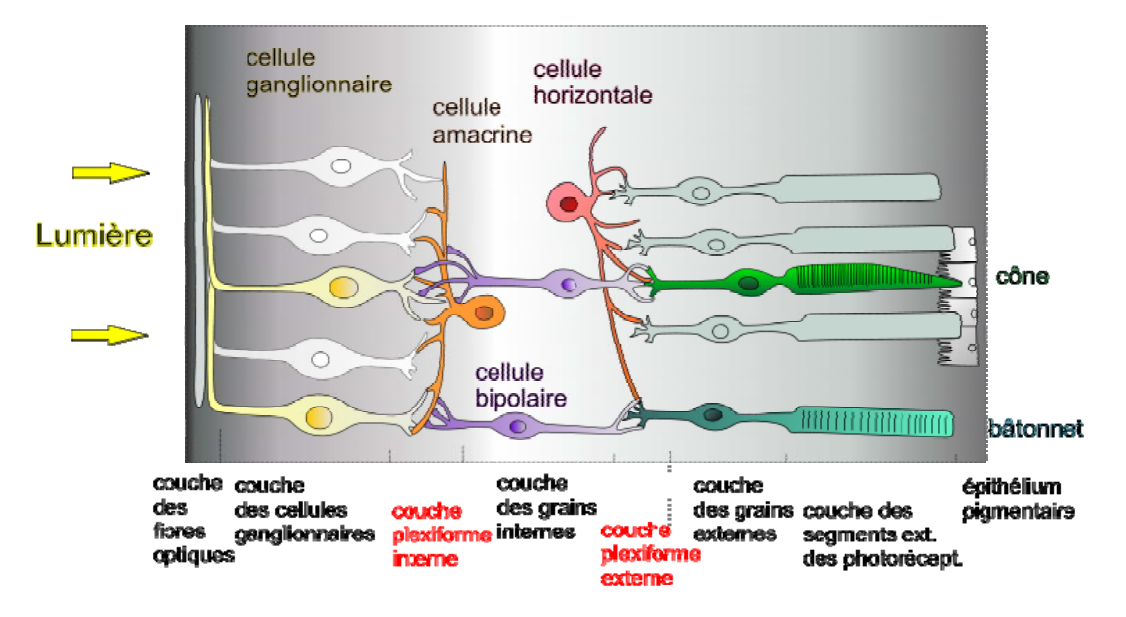
\includegraphics[scale=.45]{Figures/StructureRetinae}
		\caption{Structure et cellules composant la rétine, image tirée de  \citep{anses_effets_2014}.}
		\label{fig:structure_retine}
	\end{figure}
	
	\par Une fois le signal lumineux transformé dans une des trois voies (M, P ou M-non P), l'information circule dans le nerf optique en direction du cerveau. Les nerfs optiques de chaque œil se croisent au niveau du chiasma optique avant de continuer leur chemin dans le tractus optique et d'arriver au cerveau. Au niveau du chiasma, les fibres porteuses des informations visuelles sont redirigées: les fibres des deux moitiés gauches des yeux sont envoyées à la partie droite du cerveau, tandis que les fibres des deux moitiés droites des yeux sont envoyées à la partie gauche.
	
	\par L'interface entre le cerveau à proprement parler et le tractus optique s'appelle le CGL (Corps Genouillé Latéral). Le CGL est composé de 6 couches qui vont permettre la distribution de l'information dans les différents cortex visuels. Les informations issues de la voie M sont attribuées aux couches 1 et 2 du CGL, tandis que les informations de la voie P sont attribuées aux couches 3, 4, 5 et 6 du CGL. Les 5\% d'informations restantes (la voie M non P) ne va pas dans le CGL (et donc dans les cortex d'analyse de l'image) mais se dirige dans la mésencéphale et l'hypothalamus. Ces deux dernières aires du cerveau sont dédiées à la gestion du reste du corps humain: régulation du bio-rythme, sécrétion des hormones du sommeil, gestion de l'attention, ...
	
	\par La radiation optique permet de faire le lien, via des neurones, entre les 6 couches du CGL et le Cortex Visuel Primaire (V1) qui marque l'entrée dans le cerveau à proprement parler.
	
	\par Le traitement et la compréhension véritable des informations qui ont transité de l'œil jusqu'au CGL se fait dans les cortex visuels. La cartographie et la compréhension du fonctionnement en cortex dans le cerveau fait l'objet de plusieurs théories. Aux côtés des modèles hiérarchique et des agrégats, c'est l'hypothèse des deux voies \citep{ingle_two_1982, mishkin_object_1983, goodale_neurological_1991} qui prédomine. Cette hypothèse est aussi étendue au fonctionnement de l'audition. On la décrit dans le paragraphe suivant.
	
	\par Le traitement de l'image dans les cortex visuels est décomposé en deux voies, à l'image des voies P et M. A l'arrivée dans le Cortex Visuel Primaire (V1), l'information est divisée en deux boucles de traitement indépendantes: la voie dorsale (appelée aussi pariétale) et la voie ventrale (appelée aussi temporale). La voie dorsale correspond au traitement du mouvement et de la position (\guillemotleft~Where~\guillemotright), elle est constituée des cortex V1, V2, V3, V3A, MT et MST avant d'arriver dans le Cortex Pariétal Supérieur. Cette fois fonctionnement à une vitesse plutôt lente. De l'autre côté, la voie ventrale s'occupe de la gestion des forme et des couleurs (\guillemotleft~What~\guillemotright) et passe par les cortex V1, V2, VP, V4 et V8 avant d'arriver dans le lobe temporal. Cette voie fonctionne à grande vitesse \citep{dhondt_emotion_2011, kaiser_dorsal_2010}.
	
	\begin{figure}
		\centering
		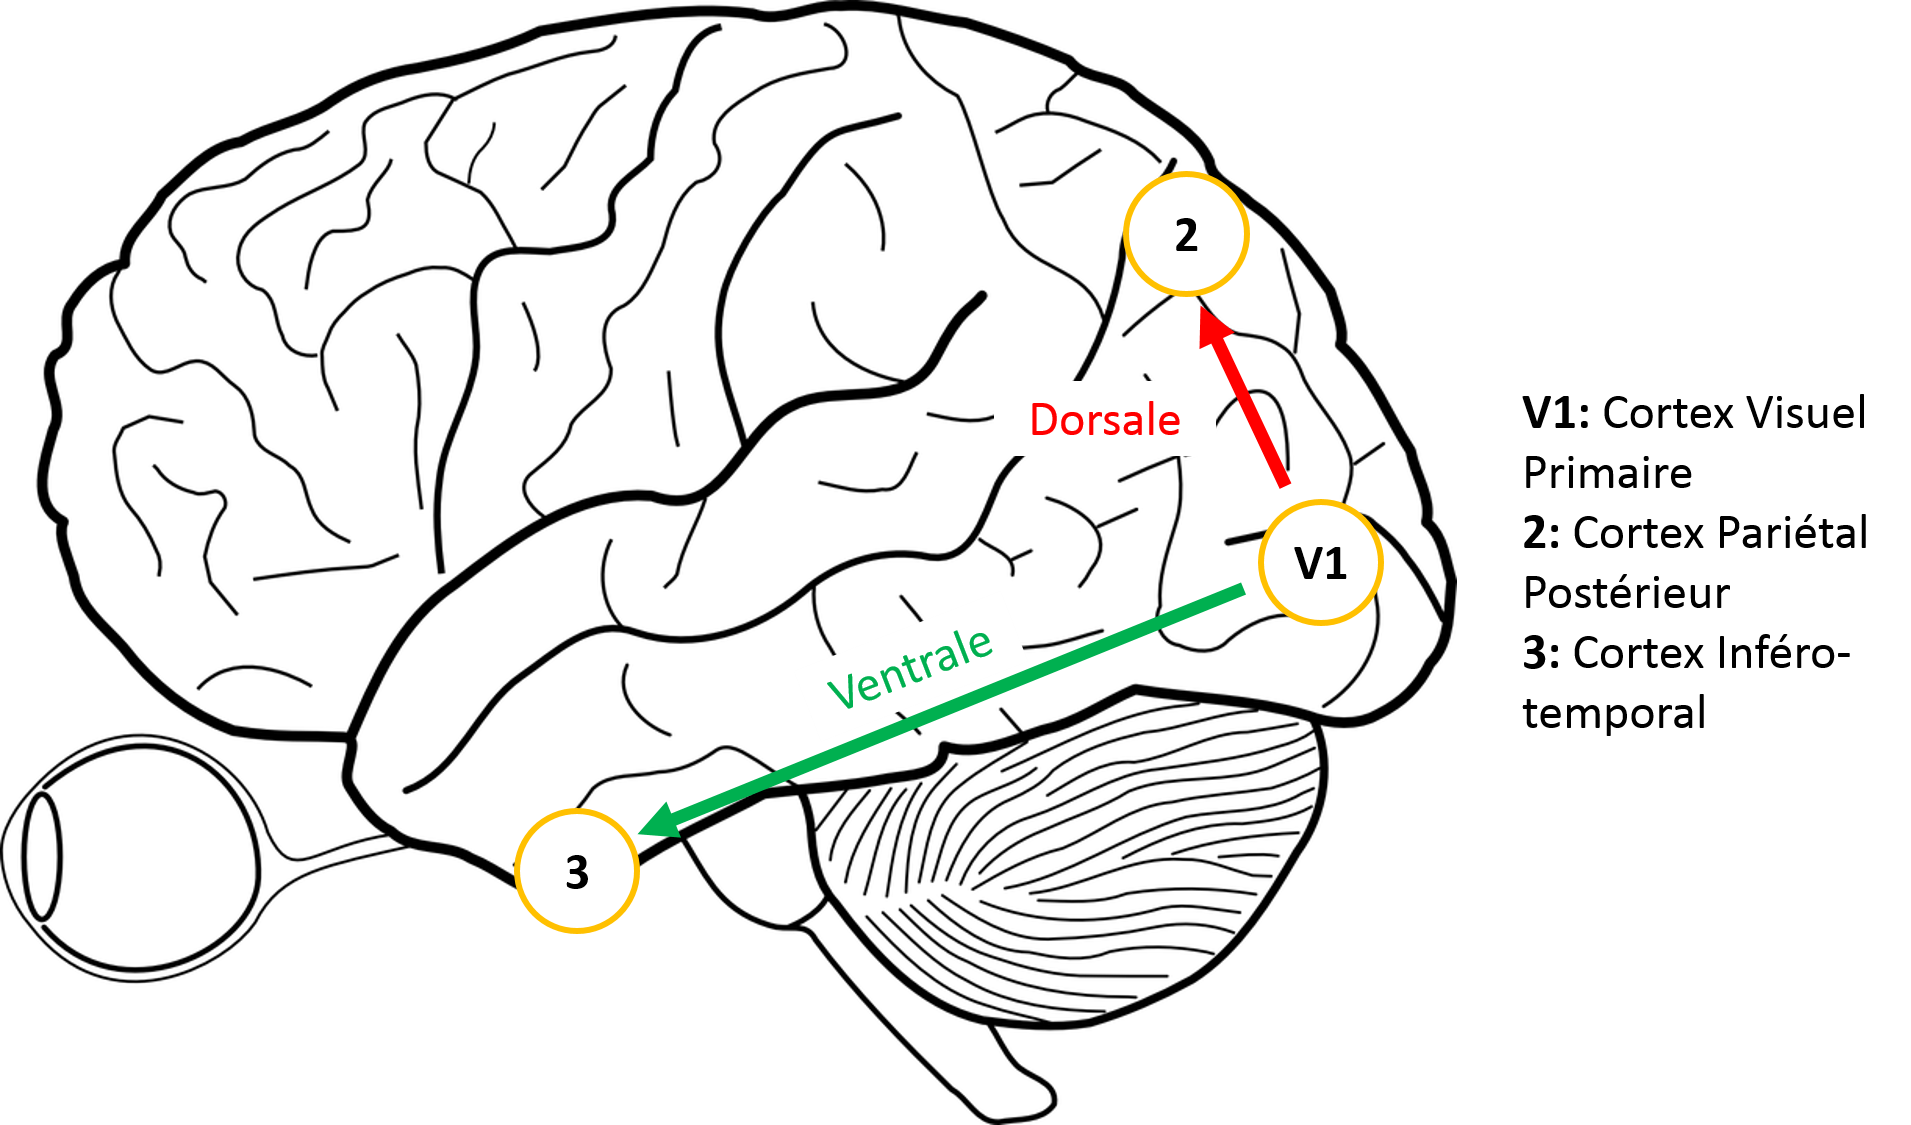
\includegraphics[scale=.35]{Figures/VoiesVentraleDorsale}
		\caption{Direction des voies ventrale et dorsale dans le cerveau.}
		\label{fig:voies_ventrale_dorsale}
	\end{figure}
	
	\par L'information visuelle n'est pas transmise au cerveau telle qu'elle sous la forme de quatre informations (bâtonnets, cônes S, cônes M, cônes L). Ces signaux de sortie des photo-récepteurs sont additionnés ou soustraits les uns entre les autres pour donner naissance à trois canaux d'information qui eux seront traités par le cerveau. Cette hypothèse de fonctionnement  -la \textit{Théorie des processus antagoniques} proposée pour la première fois par Ewald Hering en 1872- est compatible avec la théorie de la vision trichromatique (\textit{Théorie de Young-Helmholtz}, 1802 puis prouvée en 1861) puisqu'elle intervient immédiatement après dans le traitement de la lumière.
	
	\par Après les photo-récepteurs, le signal lumineux est donc découpé en trois canaux \citep{glassner_principles_1995,winkler_issues_1999}: un canal achromatique (A) et deux canaux chromatiques (R/G pour le canal rouge-vert et B/Y pour le canal bleu-jaune). On retrouvera ces canaux plus tard dans la description des espaces colorimétriques en informatique. Le canal achromatique sert à coder la valeur de luminance et est issu de la somme des signaux émis par les cônes de type M et L, $A \equiv M + L$. Le canal R/G est quand à lui la différence entre les deux précédents canaux M et L ($R/G \equiv M - L$) tandis que le canal B/Y est la différence entre les signaux émis par les cônes de type S et le canal achromatique: $B/Y \equiv S - A$. Ces mécanismes sont résumés dans la Fig. \ref{fig:opponent_colors_theory}.
	
	\begin{figure}
		\centering
		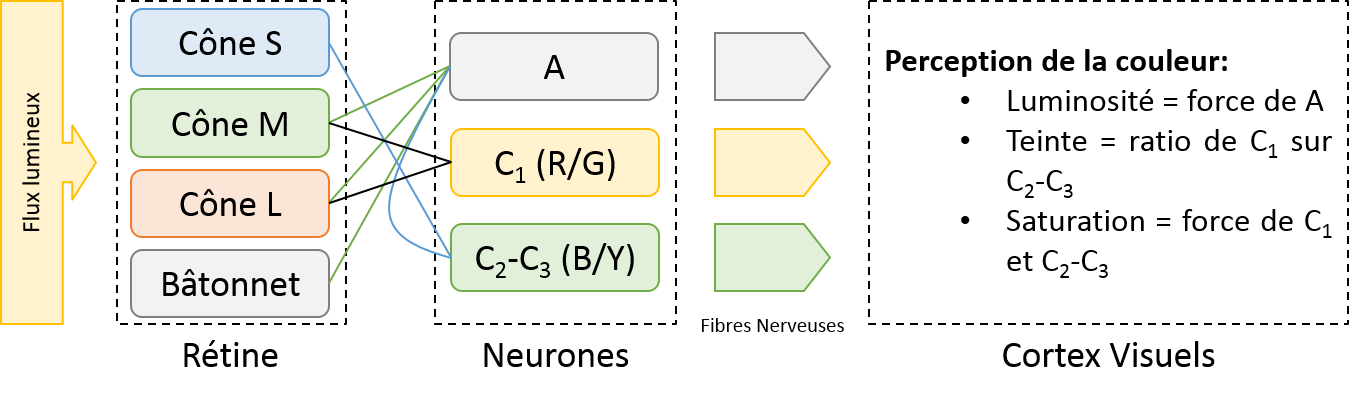
\includegraphics[scale=.6]{Figures/OpponentColorsTheory}
		\caption{Construction des canaux chromatiques et achromatique dans la théorie des processus antagoniques}
		\label{fig:opponent_colors_theory}
	\end{figure}
	
	\par Enfin, le cerveau dénote une certaine sensibilité au contraste (entendu ici comme une variation relative de luminance entre deux points de l'image perçue). Cette sensibilité dépend à la fois de la couleur (on a vu que le canal achromatique était en fait composé des retours de deux types de cônes) et à la fois des fréquences spatiales et temporelles du stimulus lumineux reçu. On peut alors établir des fonctions de sensibilité au contraste (Contrast Sensibility Functions - CSF) \citep{driscoll_eyes_1978,bezzubik_modeling_2015}. La sensibilité au contraste est définie comme l'inverse du seuil de contraste, c'est à dire le minimum nécessaire de contraste suffisant à un observateur pour détecter une variation. On peut trouver des exemples de CSF chez une grand nombre d'auteurs, comme ici avec les CSF moyennes en fonction de la fréquence spatiale du stimulus, pour différentes valeurs d'acuité visuelle (voir Fig. \ref{fig:contrast_sensitivity_functions_acuity}) \citep{owsley_contrast_1983}. On reviendra plus tard, dans une partie spécifiquement consacrée au sujet, sur la perception du contraste.
	
	\begin{figure}
		\centering
		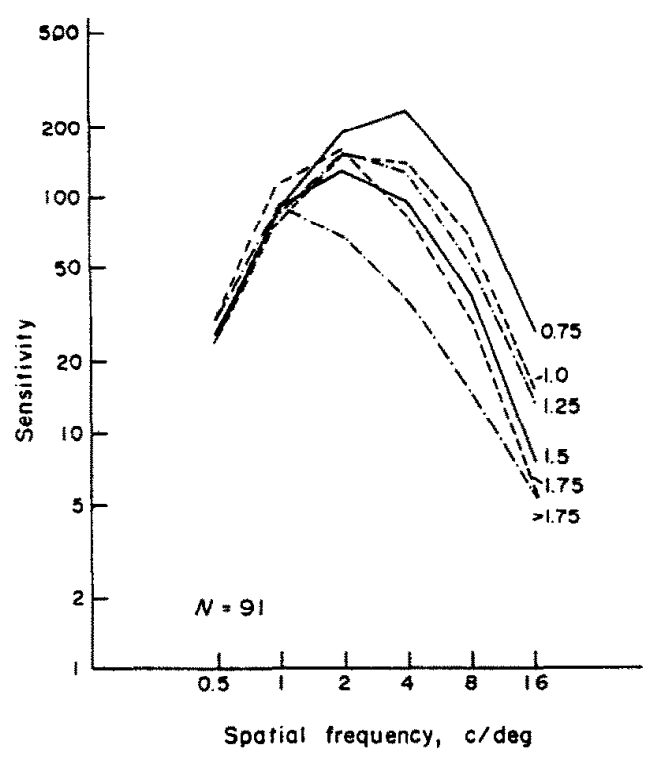
\includegraphics[scale=.45]{Figures/ContrastSensitivityFunctionAcuity}
		\caption{Courbes moyennes de sensibilité au contraste en fonction de la fréquence spatiale du stimulus pour différentes valeurs d'acuité visuelle, tiré de \citep{owsley_contrast_1983}}
		\label{fig:contrast_sensitivity_functions_acuity}
	\end{figure}
	
\chapter{Perception de la couleur}
	\par La perception de la couleur a été théorisée via un certain nombre de concepts, lois ou effets ; on présente ici les principales contributions \citep{le_grand_optique_1972, wyszecki_color_2000,judd_color_1975}. L'organisme régulateur de toutes les connaissances dans le domaine de la couleur est la CIE (ou ICE en anglais): la Commission Internationale sur l'Eclairage. En complément, on développe en annexes les différentes lois et effets qui régissent la perception de la couleur.
	
	\section{Espaces colorimétriques}
	\par Il existe de très nombreux espaces colorimétriques (sRGB, YIQ, YES, YCC, LCh, TekHVC, NCS, Munsell, Coloroid, Pantone, CIECAM97, ... \citep{beretta_understanding_2000}) mais une étude globale poussée sort très largement du cadre de l'étude. Nous nous concentrerons donc à évoquer rapidement les différents espaces principaux adoubés par la CIE.
	
	\par La première modélisation à avoir été déposée par la CIE, en 1931, est l'espace colorimétrique CIE RGB. C'est une première tentative de quantification de la couleur avec des primaires proches des maxima de réponse des cônes. La démarche est donc anthropomorphique et cherche à construire un espace linéaire. L'inconvénient (majeur) de ce système est l'obligation de passer par des composantes négatives pour certaines couleurs très saturées ; on s'éloigne alors du fonctionnement de la vision humaine qui est basée sur l'additivité des couleurs.
	
	\par Les défauts de ce premier espace ont amené la CIE à proposer dans le même temps un autre espace, le CIE XYZ, lui aussi linéaire\footnote{Linéaire: les valeurs des primaires varient linéairement, pas les couleurs perçues: une variation de primaire ne donne pas la même variation de couleur}. Dans ce modèle, Y donne	la luminance tandis que X et Z donnent la chrominance et sont définis positifs par construction.
	
	\par Mais la vision humaine des couleurs n'étant pas linéaire, un nouvel espace est développé par la CIE, en 1960, c'est le CIE UVW. Cet espace est non-linéaire et vise à améliorer l'uniformité de répartition des couleurs\footnote{Uniforme: les couleurs perçues varient de manière linéaire, au contraire de la valeur des primaires dans l'espace colorimétrique}. Dans ce modèle, la composante V correspond en tout point à la composante Y de CIE XYZ (luminance). UVW est supplanté 16 ans plus tard (1976) par CIE U'V'W' dont la variation principale est le changement de la matrice de passage vers XYZ.
	
	\par Enfin, en 1976 également, apparaissent les deux espaces les plus complets et utilisés à l'heure d'aujourd'hui: CIELAB et CIELUV. CIELUV est utilisé pour caractérisé les couleurs de lumières tandis que CIELAB sert dans le domaine des couleurs des surfaces. Ils sont basés sur U'V'W' et appartiennent à la famille des espaces uniformes mais non-linéaire. Nous détaillerons ici CIELAB car c'est celui qui est utilisé dans le domaine de l'informatique. Pour de plus amples informations, on conseillera \citep{schanda_colorimetry:_2007}.
	
	\par L'espace CIELAB, de sa vraie dénomination CIE $L^\ast a^\ast b^\ast$, est caractérisé par une composante de clarté $L^\ast$ et deux paramètres $a^\ast~et~b^\ast$ qui expriment l'écart de la couleur par rapport à une surface grise de même clarté.
	$a^\ast~et~b^\ast$ prennent leurs valeurs entre -300 et +299, 0 étant le gris de référence, mais sont en fait en général restreints entre -128 et +127 de manière à avoir 256 valeurs et être codé sur 8 bits. Le passage en couleurs codées sur 10 bits permet une nuance d'autant plus importante.
	
	\par La composante $a^\ast$ varie du vert (-300) vers le rouge (+299) tandis que la composante $b^\ast$ varie du bleu (-300) au jaune (+299) (voir Fig. \ref{fig:cielab_axes}); ce schéma est analogue au fonctionnement des canaux R-G et B-Y pour le traitement de l'image dans le cerveau.
	
	\par Le gris achromatique de référence est calculé en fonction de la lumière d'éclairage, l'illuminant choisi est en général D65, par emprunt à l'esthétique du cinéma.
	
	\begin{figure}
		\centering
		
\includegraphics[scale=1]{Figures/CIELABAxes}
		\caption{Composantes de l'espace CIELAB}
		\label{fig:cielab_axes}
	\end{figure}
	
	\par La conversion de CIEXYZ vers CIELAB se fait avec les équations suivantes \citep{robertson_historical_1990}:
	\begin{equation}
		f(x)=  \begin{cases}
		x^{1/3}, & x>\left(\frac{6}{29}\right)3\\
		\frac{1}{3}\left(\frac{6}{29}\right)^2x + \frac{4}{29}, & sinon
		\end{cases}
		\label{eq:xyz_to_lab}
	\end{equation}
	
	\par Avec $X, Y, Z$ les composantes CIEXYZ de la couleur, $X_N, Y_N, Z_N$ les composantes CIEXYZ du point blanc de référence, et:
	\begin{equation}
		\begin{cases}
		L^\ast=116 \cdot f(\frac{Y}{Y_N})-16\\
		a^\ast=500 \cdot \left[f(\frac{X}{X_N})-f(\frac{Y}{Y_N})\right]\\
		b^\ast=200 \cdot \left[f(\frac{Y}{Y_N})-f(\frac{Z}{Z_N})\right]\\
		\end{cases}
	\end{equation}
	
	\par Les valeurs des coefficients des équations de L, a et b sont en fait des valeurs approchées. Les valeurs exactes sont: \[L^\ast: 117,16~et~17.16\] \[b^\ast: 509.39\] \[b^\ast: 203,75\]
	
	\par CIELAB a aussi été traduit en coordonnées cylindriques: LCh. Les composantes C et h sont les coordonnées polaires de $a^\ast$ et $b^\ast$. Ces espaces permettent de qualifier n'importe quelle couleur indépendamment de la luminosité. 
		
	\section{Observateurs standards}
	\par Tout d'abord, il convient de (re)définir les trois domaines de vision qui correspondent à des quantités d'illumination différentes (voir Fig. \ref{fig:standard_observer_curves}) \ref{fig:photopic_mesopic_scotopic}) \citep{damelincourt_eclairage_2010}:
	\begin{itemize}
		\item La vision \textit{photopique} décrit la vision diurne (ou à haute luminosité). On entre dans le domaine \textit{photopique} à partir d'une illumination de $5~cd/m^2$.
		\item La vision \textit{scotopique} décrit la vision nocturne (ou à très basse luminosité). On entre dans le domaine \textit{scotopique} en dessous d'une illumination de $0.005~cd/m^2$.
		\item La vision \textit{mésopique} décrit la vision intermédiaire entre diurne et nocturne (luminosité basse). Le domaine \textit{mésopique} se situe pour une illumination entre $0.005~cd/m^2$ et $5~cd/m^2$.	
	\end{itemize}
	
	\begin{figure}
		\centering
		
\includegraphics[scale=1]{Figures/PhotopiqueMesopiqueScotopique}
		\caption{Répartition des domaines photopique, mésopique et scotopique}
		\label{fig:photopic_mesopic_scotopic}
	\end{figure}		
	
	\par La CIE a défini le concept d' \textit{Observateur Standard} comme un profil d'efficacité lumineuse en fonction de la longueur d'onde (voir Fig. \ref{fig:standard_observer_curves}). Chaque domaine de luminosité possède son \textit{Observateur Standard}.
	
	\begin{figure}
		\centering
		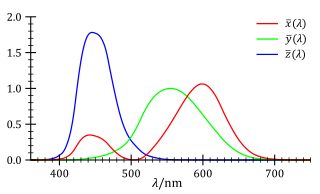
\includegraphics[scale=1]{Figures/StandardObsCurves}
		\caption{Courbes d'efficacité lumineuse des Observateurs Standards de la CIE}
		\label{fig:standard_observer_curves}
	\end{figure}
	
	\par Soit: $\begin{cases}
	\Phi_e(\lambda) & \textit{le flux énergétique en W (watts)}\\
	\Phi_v(\lambda) & \textit{le flux visuel en lm (lumen)}\\
	\lambda & \textit{la longueur d'onde en nm (nanomètres)}
	\end{cases}$
	
	\par En 1931, un premier \textit{Observateur Standard Photopique} pour le domaine photopique est mis au point. Il est noté $V(\lambda)$ et est valable pour un cône de vision de $2^\circ$, c'est à dire globalement la zone d'acuité de la fovéa. Cet observateur est révisé en 1964, en prenant en compte les résultats expérimentaux de plus de sujets pour calculer les coefficients. L'observateur est noté $V_{10}(\lambda)$ et couvre cette fois un cône de vision de $10^\circ$ \citep{le_grand_optique_1972, damelincourt_eclairage_2010}:
	\begin{equation}
		\begin{cases}
		\Phi_v(\lambda) = K_M \cdot V(\lambda) \cdot \Phi_e(\lambda)\\
		K_M = 683~lm.W^{-1}
		\end{cases}
		\label{eq:obs_photopic}
	\end{equation}
	
	
	\par L' \textit{Observateur Standard Scotopique} est quant à lui défini en 1951. Il est noté $V'(\lambda)$:
	\begin{equation}
		\begin{cases}
		\Phi_v(\lambda) = K'_M \cdot V'(\lambda) \cdot \Phi_e(\lambda)\\
		K'_M = 1700 lm.W^{-1}
		\end{cases}
		\label{eq:obs_scotopic}
	\end{equation}
	
	\par Enfin, il faut attendre 2010 pour voir apparaitre l'\textit{Observateur Standard Mésopique}, $V_{mes}(\lambda)$, qui n'est rien d'autre qu'une somme pondérée des deux autres observateurs en fonction de la luminance \citep{halonen_cie_2011}:
	\begin{equation}
		\begin{cases}
		\Phi_v(\lambda) = K_{mes} \cdot V_{mes}(\lambda) \cdot \Phi_e(\lambda)\\
		V_{mes}(\lambda) = (1-m) \cdot V'(\lambda) + m \cdot V(\lambda)
		K_{mes} = \frac{683}{V_{mes}[555)} lm.W^{-1}
		\end{cases}
		\label{eq:obs_mesopic}
	\end{equation}
	
	\par Les valeurs de $m$ sont fixées en dehors des bornes du domaine mésopique ($m = 1$ pour $L_{mes} \geq 5~cd/m^2$ et $m = 0$ pour $L_{mes} \leq 0.005~cd/m^2$), sinon elles sont calculées par récurrence \citep{halonen_cie_2011}:
	\begin{equation}		
	\begin{cases}
		m_0 = 0.5 & a = 0.7670\\
		m_n = a + b \cdot log_{10}(L_{mes,n}) & b = 0.3334\\
		L_{mes,n} = \frac{m_{n-1} \cdot L_{photopic} + (1-m_{n-1}) \cdot L_{scotopic} \cdot V'(\lambda_0)}{m_{n-1} + (1-m_{n-1}) \cdot V'(\lambda_0)} & \lambda_0 = 555 nm
	\end{cases}
	\label{eq:mesopic_param}
	\end{equation}
	
	\section{Illuminants}
	\par Les illuminants sont des standards de lumière déposés par la CIE (Commission Internationale de l'Eclairage) sous la forme de spectre de lumière visible (voir Fig. \ref{fig:illuminant_d65}). Chaque illuminant représente un certain type et une certaine couleur de lumière. Si l'illuminant D65 est le plus connu et le plus utilisé car il correspond à une lumière de midi en Europe occidentale, il existe plusieurs catégories.
	\begin{itemize}
	\item La classe A, déposée en 1931, représente une lumière moyenne d'une lampe à incandescence (filament en tungstène).
	\item La classe B (1931) représente la lumière directe émanant du soleil.
	\item La classe C (1931) représente la lumière du jour (après passage dans l'atmosphère).
	\end{itemize}

	\par Une deuxième vague d'illuminants a été adoptée plusieurs années après, à l'occasion de l'adoption du second observateur standard ($V_{10}(\lambda)$):
	\begin{itemize}
	\item La classe D (1964), qui se subdivise en plusieurs illuminants qui représentent les différentes phases de la lumière du jour, D65 étant midi.
	\item La classe E associée aux illuminants d'énergie égale (iso-énergie).
	\item La classe F représentant différentes lampes fluorescentes.
	\end{itemize}
	
	\begin{figure}
		\centering
		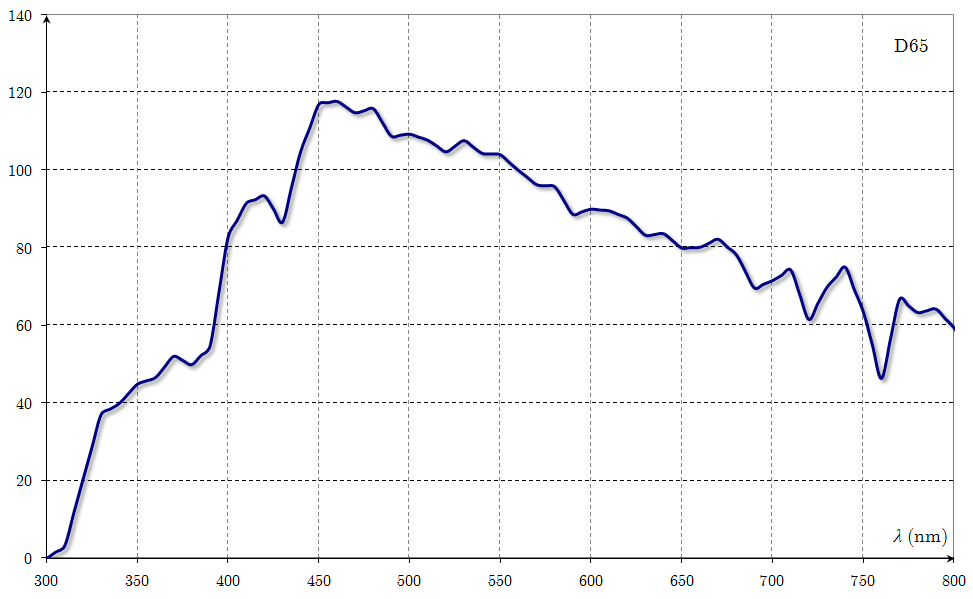
\includegraphics[scale=0.45]{Figures/IlluminantD65}
		\caption{Spectre de l'illuminant D65 (CIE)}
		\label{fig:illuminant_d65}
	\end{figure}
	
	\section{Equations de différentiations des couleurs}
	\par Une fois l'espace colorimétrique choisi, on peut dénombrer le nombre de couleurs théoriques discernables. Par exemple, dans le cas de l'espace RGB codé sur 8 bits on a 256 valeurs possibles pour chaque primaire. Lorsque l'on combine les trois primaires, on obtient un nombre théorique de 16.8 millions de couleurs. Si chacune de ces couleurs est à priori discernable, elles ne le sont pas forcément deux à deux. La CIE à donc mis en place une métrique qui indiquerait si la différence entre deux couleurs était, ou non, perceptible: $\Delta E$. Par construction, pour $\Delta E < 1$ la différence de sensation colorée n'est pas  perceptible et l'œil humain ne voit aucune différence. Empiriquement la valeur de seuil est bien plus élevée et dépend même du type de population (experte ou néophyte dans la reconnaissance de couleurs) \citep{sharma_digital_2013, vidal_color-difference_2016}.
	
	\par Il existe plusieurs équations pour calculer l'écart colorimétrique $\Delta E$, toutes ont été officialisées par la CIE en attendant des versions plus pertinentes \citep{beretta_understanding_2000, habekost_which_2013, sharma_ciede2000_2005, robertson_historical_1990}:
	\begin{itemize}
		\item CIE76
		\item CIE94
		\item CIEDE2000
		\item CMC(l,c)
	\end{itemize}
	
	\par On exprimera ici les équations dans l'espace CIELAB dans sa version originale $(L^\ast a^\ast b^\ast)$ ou dans sa version en coordonnées cylindriques $(L^\ast C h_{ab})$.
	
	\par La première équation, CIE76, est la plus simple et consiste en une simple distance euclidienne dans l'espace colorimétrique \citep{sharma_digital_2013}:
	\begin{equation}
		\Delta E_{76} = \sqrt{(\Delta L)^2 + (\Delta a)^2 + (\Delta b)^2}
		\label{eq:de_76}
	\end{equation}
	
	\par Ensuite, CIE76 a été modifiée pour s'adapter à la non linéarité de perception des couleurs \citep{beretta_understanding_2000}, elle est adoptée en 1994 et devient CIE94:
	\begin{equation}
		\Delta E^\ast_{94} = \sqrt{\left(\frac{\Delta L^\ast}{k_L \cdot S_L}\right)^2 + \left(\frac{\Delta C^\ast_{ab}}{k_C \cdot S_C}\right)^2 + \left(\frac{\Delta H^\ast_{ab}}{k_H \cdot S_H}\right)^2}
		\label{eq:de_94}
	\end{equation}
	
	\par Avec:
	$\begin{cases}
	C^\ast_{ab} = \sqrt{a^{\ast 2} + a^{\ast 2}}\\
	\Delta H^\ast_{ab} = \sqrt{\Delta E^{\ast 2}_{ab} - \Delta L^{\ast 2} - \Delta C^{\ast 2}_{ab}} = \sqrt{\Delta a^{\ast 2} + \Delta b^{\ast 2} - \Delta C^{\ast 2}_{ab}}\\
	S_C = 1 + 0.0045 \cdot C^\ast_{ab}\\
	S_H = 1 + 0.0015 \cdot C^\ast_{ab}\\
	S_L = k_L = k_C = k_H = 1
	\end{cases}$
	
	\par L'équation de 1994 résout un grand nombre de problèmes mais éprouve toujours des difficultés à décrire parfaitement le comportement de l'oeil, notamment dans le bleu. Une troisième équation est donc officialisée en 2000, CIEDE2000 \citep{schanda_colorimetry:_2007, sharma_ciede2000_2005}:
	\begin{equation}
		\Delta E^\ast_{00} = \sqrt{\left(\frac{\Delta L'}{k_L \cdot S_L}\right)^2 + \left(\frac{\Delta C'}{k_C \cdot S_C}\right)^2 + \left(\frac{\Delta H'}{k_H \cdot S_H}\right)^2 + R_T \cdot \frac{\Delta C'}{k_C \cdot S_C} \cdot \frac{\Delta H'}{k_H \cdot S_H}}
		\label{eq:de_2000}
	\end{equation}
	
	\par Le détail des coefficients de $\Delta E^\ast_{00}$ (complexe et hors de propos ici) est disponible notamment sur le site de Bruce Lindbloom\footnote{Bruce Lindbloom, \textit{Delta E (CIE 2000)}, \url{http://brucelindbloom.com/index.html?Eqn_DeltaE_CIE2000.html} (Juillet 2016)}.

	\par Enfin, si CIEDE2000 donne de très bon résultats lorsqu'il faut discriminer des couleurs de manière objective, c'est une autre équation, DECMC qui semble plus appropriée pour une discrimination subjective/perceptuelle \citep{habekost_which_2013}:
	\begin{equation}
		\Delta E(l,c) = \sqrt{\left(\frac{\Delta L}{l \cdot S_L}\right)^2 + \left(\frac{\Delta C}{c \cdot S_C}\right)^2 + \left(\frac{\Delta H}{S_H}\right)^2}
		\label{eq:de_cmc}
	\end{equation}
	
	\par Avec:
	$\begin{cases}
	(l,c) = (2,1) & \textit{pour l'acceptabilité}\\
	(l,c) = (1,1) & \textit{pour la perceptibilité}
	\end{cases}$
	
	\par De même que pour CIEDE2000, le détail des coefficients de $\Delta E(l,c)$ est disponible sur le site de Bruce Lindbloom\footnote{Bruce Lindbloom, \textit{Delta E (CMC)}, \url{http://brucelindbloom.com/index.html?Eqn_DeltaE_CMC.html} (Juillet 2016)}. On revient maintenant plus en détails sur la perception du contraste.

\chapter{Contraste}
	\section{Définitions mathématiques}
	\par Tout d'abord, le dictionnaire définit le contraste comme une <<~opposition de deux choses, l'une faisant ressortir l'autre~>>\footnote{Contraste. (s.d.). Dans \textit{Dictionnaire Larousse en ligne}. Repéré à \url{http://www.larousse.fr/dictionnaires/francais/contraste/18688}}. On trouve également deux définitions plus spécifiques que sont le contraste des couleurs\footnote{Contraste des couleurs. (s.d.). Dans \textit{Dictionnaire Larousse en ligne}. Repéré à \url{http://www.larousse.fr/dictionnaires/francais/contraste/18688/locution}}: <<~effet subjectif d'une apposition quantitative de couleurs, par exemple des stimulations sensorielles juxtaposées dans l'espace (contraste simultané) ou dans le temps (contraste successif)~>> et le contraste d'une image optique\footnote{Contraste d'une image optique. (s.d.). Dans \textit{Dictionnaire Larousse en ligne}. Repéré à \url{http://www.larousse.fr/dictionnaires/francais/contraste/18688/locution}}: <<~variation relative de l'éclairement d'une image lorsqu'on se déplace à l'intérieur de cette image~>>. L'opposition se ferait ici entre le blanc et le noir pour avoir la valeur maximale du contraste.
	
	\par Ces définitions sont toutefois insuffisantes ou tout du moins inutilisables dans le monde de la vision et de l'imagerie informatique. Il faut alors théoriser plus précisément le concept de contraste et le représenter mathématiquement pour pouvoir à la fois le mesurer et le caractériser.
	Il existe pour ce faire au moins 3 méthodes analytiques, résumées ci-après:
	\begin{itemize}
		\item Le contraste de Michelson \citep{michelson_studies_1995,winkler_issues_1999,fuchs_traite_2003}.
		\item Le contraste de Weber \citep{winkler_computing_1999,winkler_issues_1999}.
		\item Le contraste de Peli \citep{peli_contrast_1990,winkler_computing_1999,winkler_issues_1999}.
	\end{itemize}

	\par Premièrement, le contraste de Michelson est défini par l'Eq. \ref{eq:contrast_michelson}, avec $L_{max}$ la valeur maximale de la luminance de l'image, et $L_{min}$ la valeur minimum. Le contraste de Michelson prend ses valeurs dans l'intervalle $\left[0;1\right]$.
	\begin{equation}
	C_{Michelson}=\frac{L_{max}-L_{min}}{L_{max}+L_{min}}
	\label{eq:contrast_michelson}
	\end{equation}

	\par Le contraste de Weber est quant à lui défini tel que dans l'Eq. \ref{eq:contrast_weber}, $\Delta L$ étant la plus petite différence de luminance visible, pour une luminance $L$ donnée. A la différence du contraste de Michelson, le contraste de Weber prend ses valeurs dans l'intervalle $\left[-1;+\infty\right[$.
	\begin{equation}
	C_{Weber}=\frac{\Delta L}{L}
	\label{eq:contrast_weber}
	\end{equation}
	
	\par Enfin, Peli a proposé un modèle de contraste pour les images complexes basé sur une analyse fréquentielle de l'image (Eq. \ref{eq:contrast_peli}). Avec $BP_{i}(x,y)$ la bande passante de l'image $i$ et $LP_{i}(x,y)$ l'énergie sous la fréquence de coupure.
	\begin{equation}
	C_{i}(x,y) = \frac{BP_{i}(x,y)}{LP_{i}(x,y)}
	\label{eq:contrast_peli}
	\end{equation}
	
	\par Malgré tout, il n'existe pas (encore) de méthode parfaite et définitive pour mesurer le contraste dans les images complexes de type image de simulateur \citep{winkler_computing_1999}. Les définitions analytiques vues à l'instant sont valables pour des images très simples et statiques.
	
	\section{Calcul de seuil}
	\subsection{Cas général}
	\par Le calcul du contraste en lui même ne suffit pas, il faut aussi savoir comment celui évolue en fonction de la luminance de l'écran: il semble assez naturel qu'à très forte luminance la capacité à distinguer un certain niveau de contraste ne soit pas la même qu'à très faible luminance. On recense ici trois modèles de comportement pour le contraste issus de la littérature:
	\begin{itemize}
		\item La fraction de Weber\footnote{Serge Bertorello, \textit{Notions d'Optique - La Vision}, \url{http://serge.bertorello.free.fr/optique/vision/vision.html} (Juillet 2016)}.
		\item Le modèle de Blackwell \citep{international_commission_on_illumination_analytic_1981}.
		\item Le modèle de Ward \citep{heckbert_contrast-based_1994}.
	\end{itemize}
	
	\par Ces modèles, notamment la fraction de Weber, ne sont souvent parfaitement valables que dans le domaine photopique (lumière du jour) et sont beaucoup plus fragiles en conditions mésopique (basse luminosité) ou scotopique (luminosité nocturne). Ils sont donc à utiliser avec prudence.

	\par Surement le modèle le plus connu, la fraction de Weber est dans la continuité du contraste de Weber définit précédemment. Si il s'applique notamment au contraste, ce modèle est en fait utilisable pour n'importe quel type de stimulus et est assez général. La fraction est simplement posée telle que dans Eq. \ref{eq:contrast_weber_fraction}, avec $k$ une constante, $\Delta I$ la plus petite différence d'intensité perceptible et $I$ l'intensité du stimulus. La valeur de $k$ est généralement admise à $0.02$.
	
	\begin{equation}
	\frac{\Delta I}{I} = k = 0.02
	\label{eq:contrast_weber_fraction}
	\end{equation}
	
	\par De cette fraction de Weber est issue une autre loi à propos du comportement de la rétine face à une intensité lumineuse, la loi de Weber-Fechner (Eq. \ref{eq:contrast_weber_fechner_law}). Avec $S$ la sensation perçue, $I$ l'intensité de la stimulation et $k$ une constante.
	
	\begin{equation}
	S = k \cdot log(I)
	\label{eq:contrast_weber_fechner_law}
	\end{equation}
	
	\par En 1981, la CIE a adopté un modèle établi par Blackwell et destiné au comportement du contraste en fonction de la luminance uniquement. Ce modèle donne la plus petite différence de luminance perceptible $\Delta L$ pour une luminance moyenne donnée $L_{a}$ (Eq. \ref{eq:contrast_blackwell_model}). Ici, $L_{a} \pm \Delta L$ est perceptible tant que $L_{a} \pm \epsilon$ alors $\epsilon < \Delta L$ ne l'est pas.
	
	\begin{equation}
	\Delta L(L_{a}) = 0.0594 (1.219 + L_{a}^{0.4})^{2.5}
	\label{eq:contrast_blackwell_model}
	\end{equation}
	
	\subsection{En Réalité Virtuelle}
	\par Le modèle de Ward donne un lien direct (linéaire) entre la différence minimale perceptible de luminance qui serait perçue dans le monde réel ($L_{wa}$) et sont équivalent sur un dispositif d'affichage $L_{da}$ (Eq. \ref{eq:contrast_ward_model}). Le coefficient de linéarité $m$ est donné par l'Eq. \ref{eq:contrast_ward_model_m}.
	
	\begin{equation}
	\Delta L(L_{da}) = m \cdot \Delta L(L_{wa})
	\label{eq:contrast_ward_model}
	\end{equation}
	
	\begin{equation}
	m = {\left[ \frac{1.219 + (L_{da})^{0.4}}{1.219 + (L_{wa})^{0.4}} \right]}^{2.5}
	\label{eq:contrast_ward_model_m}
	\end{equation}
	
	\par Une fois ces modèles analytiques mis en place, on se rend compte assez facilement de leur lourdeur et de incapacité à s'adapter à des situations concrètes, notamment dans le domaine le l'informatique temps réel. Nous verrons donc dans un prochain chapitre d'autres pistes et d'autres moyens plus pratiques de quantifier le contraste.
	
	\section{Méthodes classiques de calcul sur un écran}
	\par Une première méthode classique de mesure du contraste sur un écran est la méthode dite <<~ON/OFF~>>. Elle consiste à mesurer la luminance produite par une écran lorsque celui-ci émet sa luminance maximale (c'est à dire pour un écran affiché entièrement blanc) puis la luminance minimum émise (pour écran affiché entièrement noir) et d'en faire le ratio. Si elle permet de mesurer le plus gros écart de luminance possible elle est trompeuse lorsqu'il s'agit de caractériser un écran: l'alternance noir-blanc ou blanc-noir n'était pas représentative de l'usage réel et les (futurs) utilisateurs de l'écran ne seront jamais en situation de percevoir un tel écart.
	
	\par Pour prendre en compte cette différence avec la réalité, une autre technique a été mise au point, la méthode dite ANSI (comme l'organe de régulation américain <<~American National Standards Institute~>>). Pour représenter la luminance moyenne des images habituellement affichées sur l'écran, on ne mesure plus sur des surfaces monochromes mais sur un damier noir et blanc de 4 par 4. On fait alors le ration entre la moyenne des luminances des blancs sur la moyenne des luminances des noirs. De cette manière, les zones blanches de l'écran influent sur les zones noires en augmentant leur luminance, et inversement.
	
\chapter{Perception visuelle de la profondeur}
	\par La perception de la profondeur est une des composantes fondamentales de la vision et doit faire partie des critères d'une immersion réussie. Cette perception passe par un certain nombre de principes et de paradigmes à la fois monoculaires (fonctionnement grâce à un seul œil) ou binoculaire (fonctionnement nécessairement avec les deux yeux). Les indices de profondeurs utilisés par le cerveau sont les suivants, et sont résumés et ordonnés dans la Fig. \ref{fig:indices_profondeur}:
	\begin{itemize}
	\item l' accommodation,
	\item la vergence,
	\item les disparités (horizontale et verticale),
	\item la parallaxe,
	\item les indices statiques: interposition, taille, perspective linéaire, gradient de texture, perspective aérienne, ombre, ...
	\end{itemize}
	
	\begin{figure}
		\centering
		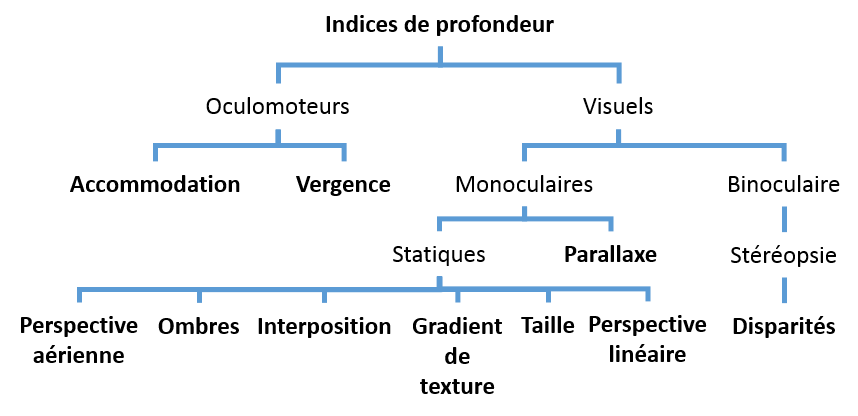
\includegraphics[scale=1]{Figures/IndicesProfondeur}
		\caption{Indices visuels de perception de la profondeur}
		\label{fig:indices_profondeur}
	\end{figure}
	
	\par Premièrement, le cerveau peut récupérer assez facilement les informations d' \textit{accommodation} et de \textit{vergence} via le principe dit de \textit{proprioception} évoqué plus haut. En récupérant des informations sur les muscles oculomoteurs le cerveau en déduit l'état de vergence et d' accommodation puis des informations sur la proximité de l'objet sur lequel est concentré le regard. En effet, une accommodation et une vergence à l'infini signifieront un objet éloigné et inversement. Ces indices ne sont ni les plus forts ni les plus robustes mais participent à un tout.
	
	\par La différence de disparité entre deux points permet au cerveau de comparer leurs positions respectives. Au niveau technologique cet indice est apporté par la stéréoscopie. Pour plus d'informations sur l'indice binoculaire de profondeur, on pourra se reporte à \citep{glassner_principles_1995}.
	
	\par La \textit{parallaxe}, ou parallaxe de mouvement, est un indice temporel, c'est à dire qu'il ne fonctionne pas à un instant $t$ donné mais plutôt sur une période de temps $\Delta t$. En effet, la parallaxe est l'effet sur le cerveau d'un changement de point de vue: le cerveau analyse les différences entre les images $n$ et $n+1$, et, en fonction des quantités et des vitesses de déplacement en déduit la profondeur des objets. Lorsque qu'un observateur bouge la tête en gardant le même point de fixation, tous les objets entre le point de fixation et l'observateur vont bouger avec un gradient de vitesse basé sur la distance au point de fixation (plus l'objet est éloigné, plus il va vite). Tous les points derrière le point de fixation bougeront aussi mais avec un gradient de vitesse opposé. Technologiquement, la parallaxe est assurée par la capture et l'intégration du mouvement de la tête et/ou des yeux de l'observateur dans le calcul de l'image.
	
	\par Parmi les indices statiques, l'\textit{interposition} (ou occultation) est assez simple et révélateur: si un objet masque (partiellement) un autre, alors l'objet masqué à une profondeur supérieure à l'objet masquant. Cet indice est notamment très utilisé en informatique graphique dans le pipeline de rendu\footnote{Pour plus d'informations sur le pipeline de rendu: \textit{Rendering Pipeline Overview}, \url{https://www.opengl.org/wiki/Rendering_Pipeline_Overview} (Juillet 2016, en anglais).} au moment de calculer une image: tous les objets masqués sont ignorés pour le rendu de l'image (ce qui permet un gain de temps, notamment sur des scène complexes) et les objets partiellement masqués voient leur géométrie modifiée afin de ne garder que la (les) partie(s) visible(s).
	
	\par La \textit{taille} est un autre indice, basé cette fois sur notre expérience d'objets familiers dont on connais ou dont on visualise la taille. Si une voiture est vue minuscule, par expérience, on déduira que la voiture est donc loin. Cet indice ne marche qu'avec des objets que l'on connait déjà et peut être berné assez facilement (comme par exemple avec l'illusion d'optique de la chambre d'Ames).
		
	\par L'\textit{ombre} permet localement de donner des indices flagrants sur la profondeur de l'objet (voir Fig. \ref{fig:profondeur_perspectives}).
	
	\par Enfin il existe un certain nombre d'indices statiques monoculaires \citep{glassner_principles_1995, fuchs_traite_2003} que l'on peut regrouper sous la dénomination \guillemotleft~Perspective~\guillemotright . Certains de ces différents types de perspective sont illustrés Fig. \ref{fig:profondeur_perspectives}:
	\begin{itemize}
		\item Le \textit{gradient de texture} consiste à un rapprochement apparent (un écrasement des distances relatives) entre les objets de plus en plus lointains.
		\item La \textit{perspective aérienne} fonctionne pour les grandes distances uniquement: plus un objet va s'éloigner de l'observateur, plus sa couleur va perdre en intensité et fondre vers le bleu-gris (couleur de l'atmosphère), typiquement le cas des montagnes ou d'un paysage que l'on voit à l'horizon.	
		\item La \textit{perspective linéaire} est la perspective bien connue avec lignes de fuite: plus un objet s'éloigne, plus il semble rapetisser.
	\end{itemize}
	
	\par Nous avons vu le fonctionnement de la vision (modélisation du système visuel, perception de la couleur et du contraste), et son interprétation (perception de la profondeur). Néanmoins, toutes ces connaissances ne s'applique que dans le cas d'un sujet parfait. Nous allons maintenant présenter quelques facteurs humains (physiologiques) qui peuvent venir dégrader ou modifier la vision et ses performances.	
	
	\begin{figure}
		\centering
		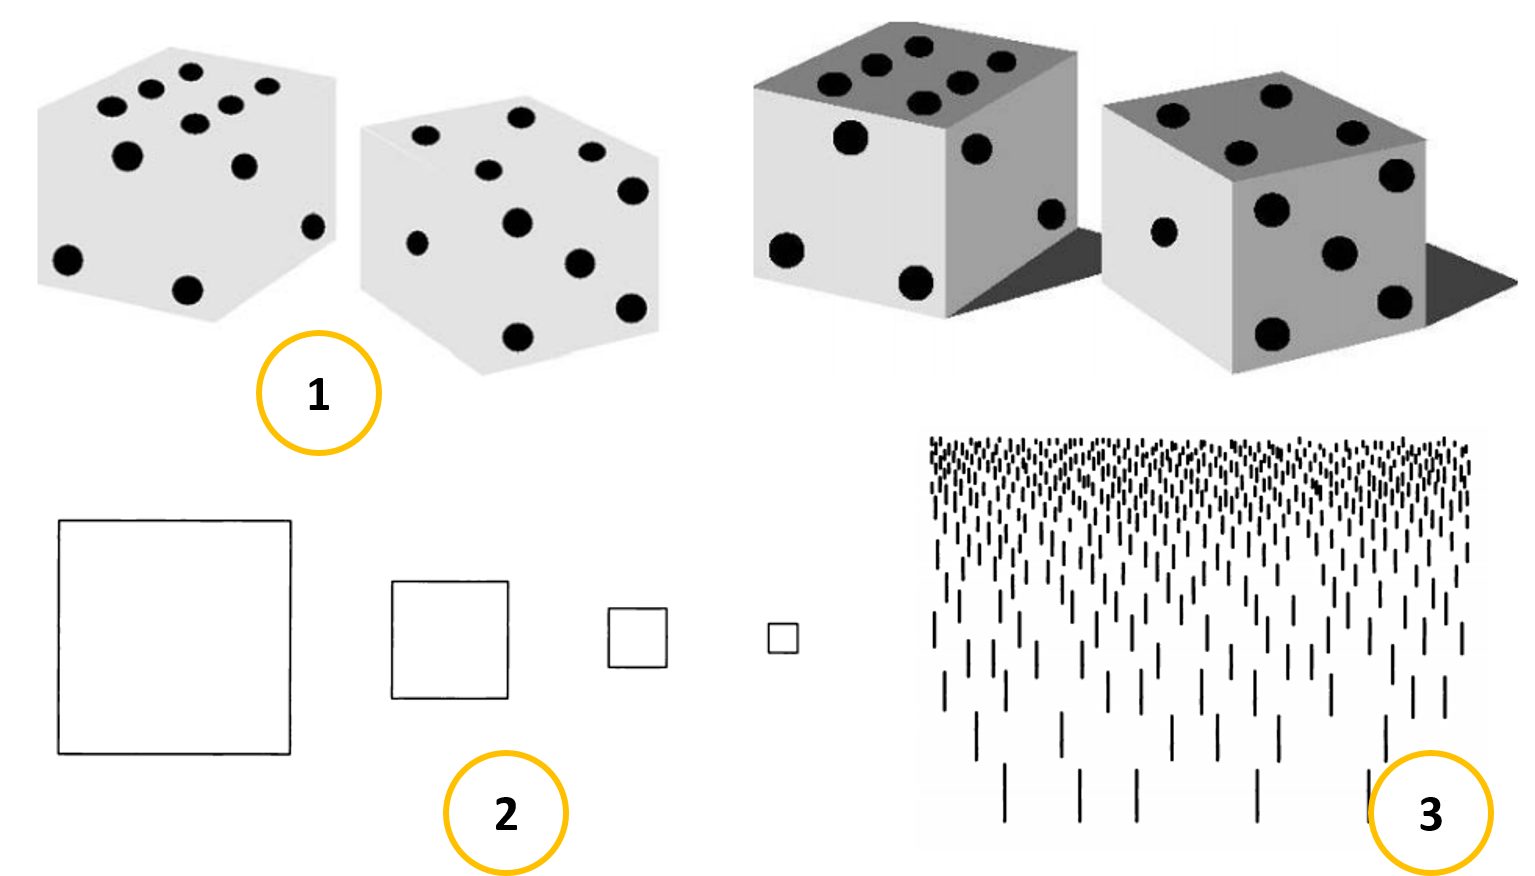
\includegraphics[scale=.25]{Figures/PerspectivesProfondeur}
		\caption{Illustration d'indices de profondeur: ombres (1, image tirée de \citep{anses_effets_2014}), taille (2) et gradient de profondeur (3, images tirées de \citep{glassner_principles_1995}).}
		\label{fig:profondeur_perspectives}
	\end{figure}
	
\chapter{Influences Physiologiques}
	\par Outre les maladies ou autres défauts oculaires qui ne seront pas abordés ici, il existe un certain nombre de paramètres liés au corps humain qui influent sur la qualité de perception des images projetées par le dispositif immersif d'affichage. On trouve principalement des influences morphologiques (au niveau du visage) ou d'âge de l'observateur. On peut noter que la sensibilité au contraste est dépendante des conditions d'expérimentations évidemment, de facteurs ophtalmologiques (myopie, éblouissement rétinien, cataracte, amblyopie, dégénération de la macula avec l'âge, hyper-tension oculaire, glaucome, sécheresse oculaire) mais aussi de facteurs neurologiques (lésions cérébrales, scléroses, maladie de Parkinson et schizophrenie), ou encore de facteurs liés à la prise de médicaments \citep{pelli_measuring_2013}. Nous nous plaçons évidemment dans le cas où le sujet est sain.
		
	\section{Variations morphologiques}
	\par Les influences morphologiques sont très nombreuses au niveau du visage et plus ou moins faciles à caractériser et à traiter. On retrouve par exemple la distance inter-oculaire (distance entre le centre des pupilles), profondeur des yeux, non-horizontalité de l' alignement du centre des pupilles, glissement des lunettes pendant l'utilisation, position des oreilles par rapport au nez pour la poste des lunettes 3D, écart de position entre une première et une seconde mise de lunettes, la position du casque immersif sur le visage ... tout ce qui fait de l'observateur humain un observateur symétriquement et géométriquement imparfait.
	
	\par On développera ici le cas simple de la distance inter-oculaire. Il apparait que lorsque l'on présente les mêmes images stéréo à deux personnes différentes, la profondeur stéréoscopique des objets proches n'est pas perçue de manière égale. On prend l'exemple de l'image d'un volant de virtuel normalement paramétré pour apparaitre confondu avec le volant réel du simulateur de conduite. Certain utilisateurs verrons effectivement le volant là où il est sensé être, tandis que d'autres verront l'image légèrement en avant du volant et d'autres la verront légèrement en retrait. Cet écart peut être extrêmement gênant et s'explique notamment par l'écart de distance inter-pupillaire entre les différents observateurs. Il serait cependant intéressant de comparer l'influence des différentes influences physiologiques vues précédemment afin de les hiérarchiser et éventuellement d'en négliger certaines.
	
	\par Les grandeurs ici évoquées font référence à la Fig. \ref{fig:profondeur_stereo_dio}. Pour un individu A qui a une distance interoculaire $e$, on projette sur les murs du CAVE, où dans un visio-casque, à distance $D$, un couple d'images stéréoscopiques (ici représentées par les segments rouge et bleu). L'image reconstruite par le cerveau est vue à une distance $d$ par l'individu. Les images œil gauche et œil droit sont dissociées d'une distance $y$. En gardant les mêmes images, un individu B avec une distance interoculaire $e\prime$ se positionne au même endroit dans le CAVE. C'est à ce niveau là qu'intervient la différence de perception, et le second individu verra l'objet virtuel non pas à une distance $d$ mais à une distance $d\prime$ qui peut être supérieure ou inférieure à $d$.

	\begin{figure}
		\centering
		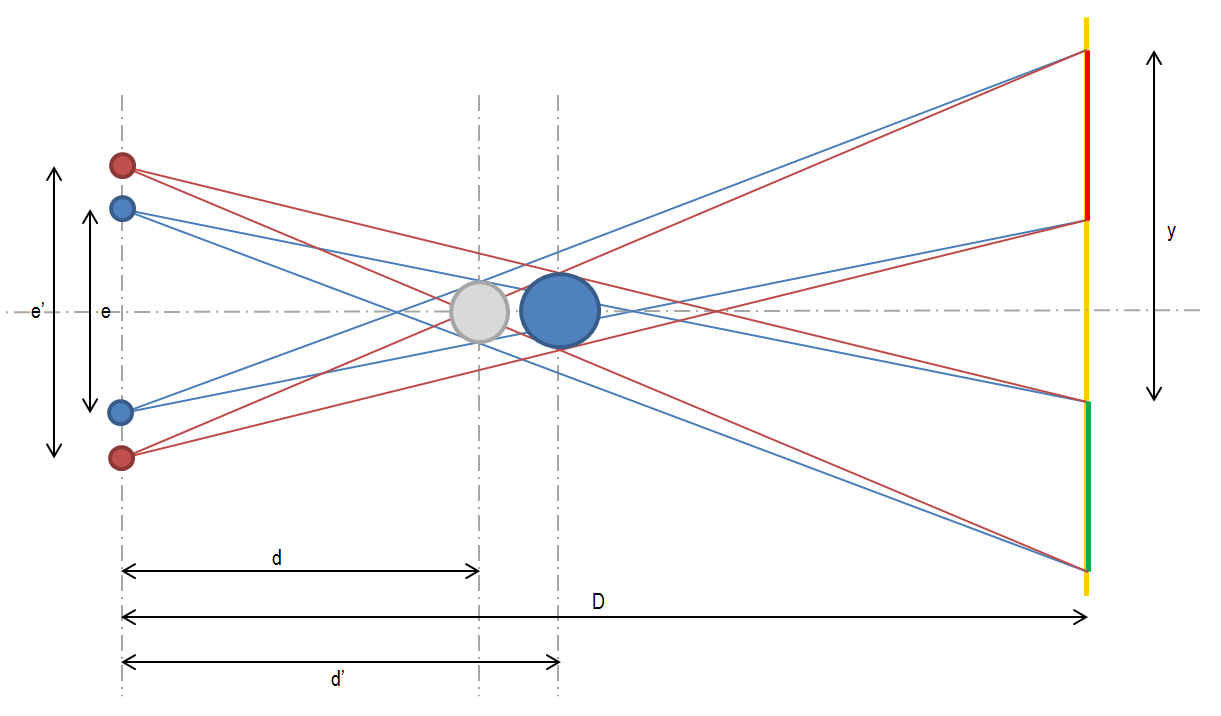
\includegraphics[scale=.5]{Figures/ProfondeurStereoDIO}
		\caption{Schématisation de la différence de profondeur stéréoscopique perçue en fonction de la distance interoculaire}
		\label{fig:profondeur_stereo_dio}
	\end{figure}

	\par En utilisant les règles élémentaires de trigonométrie (et après simplification), on trouve que la différence de distance de l'objet virtuel entre les deux individus se note de la manière suivante (Eq. \ref{eq:difference_distance_dio}):
	\begin{equation}
		\Delta d = \frac{(D - d)(e + \Delta e) - y \cdot d}{y + e + \Delta e}
		\label{eq:difference_distance_dio} 
	\end{equation}
	
	\par La Fig. \ref{fig:abaque_dio} est un abaque partiel pour une configuration donnée et pour le spectre des distances inter-oculaires possibles, de l'écart de profondeur perçue entre l'observateur A et l'observateur B pour un même jeu d'images stéréoscopiques.
	
	\par L'abaque est tracé dans la configuration spécifique avec des images projetées à la distance $D = 1.5~m$ et pour des distances de perception de l'objet en 3D de $d = 50~cm$, $75~cm$, $1~m$ et $1~m~25$. De même, on se place dans le cas général, et dans les pratiques usuelles en 3D échelle $1:1$, la distance interoculaire initiale (individu A) utilisée pour calculer le couple d'images stéréoscopiques est de 64 mm, qui est la distance interoculaire moyenne chez les hommes \citep{dodgson_variation_2004}.
	
	\par Dans le cas idéal, celui où la distance inter-oculaire n'influerait pas sur la perception de la profondeur, les images calculées pour $64~mm$ (trait orange vertical) seraient vues toujours à la même distance quelque soit la distance interoculaire (traits horizontaux en pointillés). Mais la géométrie montre bien que la réalité est tout autre (traits pleins).
	
	\par Les résultats qui émergent des courbes sont les suivants: si l'individu A perçoit l'objet virtuel à une distance de $1~m$ (courbes rouges, voir \ref{fig:abaque_dio}), un individu B avec une distance oculaire de $60~mm$ (distance inter-oculaire moyenne chez les femmes \citep{dodgson_variation_2004}) verra le même objet virtuel à $980~mm$ (donc légèrement plus proche), soit avec un écart de $2~cm$ par rapport à l'observateur calculé.
	
	\begin{figure}
		\centering
		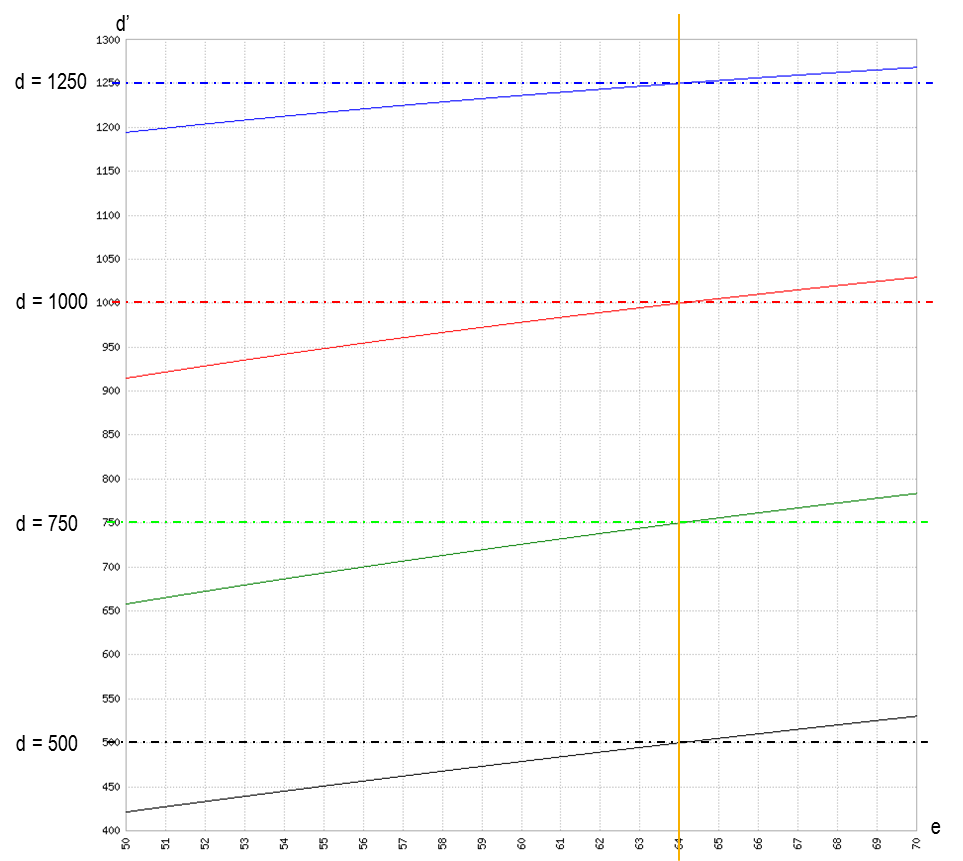
\includegraphics[scale=.8]{Figures/AbaqueDIO}
		\caption{Abaques de la nouvelles distance perçue en fonction de la distance inter-oculaire}
		\label{fig:abaque_dio}
	\end{figure}
	
	\section{Âge}
	\par L'ergonomie du système d'affichage et la physionomie du visage ne sont pas les seuls facteurs influençant la perception. Un certain nombre d'autres paramètres entrent en jeu, comme notamment le genre (homme ou femme) pour la vision des couleurs \citep{fairchild_human_2005} mais surtout, pour la quasi totalité des grandeurs de la vision: l'âge de l'observateur.
	
	\par On peut dès lors évoquer la modification, avec l'accumulation des années, de facteurs comme le diamètre pupillaire, l'acuité visuelle ou la sensibilité au contraste \citep{owsley_contrast_1983} (voir Fig. \ref{fig:contrast_sensitivity_functions_acuity}), la réduction de la capacité à extraire des informations dans le champ de vision \citep{sekuler_effects_2000,ball_age_1988,roge_influence_2004, roge_deterioration_2009,gross_human_2008}, la qualité de l'image rétinienne \citep{artal_effects_1993}, la densité de cônes dans la fovéa \citep{kilbride_foveal_1986}, le structure de l'œil et du cristallin \citep{cook_aging_1994}.
	
	\par Par ailleurs, on note les excellentes vidéos de Craig Blackwell sur le thème du vieillissement de l'œil et de la vision\footnote{Craig Blackwell. 3 décembre 2014. Aging Eye 1: Vision [Vidéo en ligne]. Repéré à https://www.youtube.com/watch?v=FtcZ4an-VGo}.
	
	\begin{figure}
		\centering
		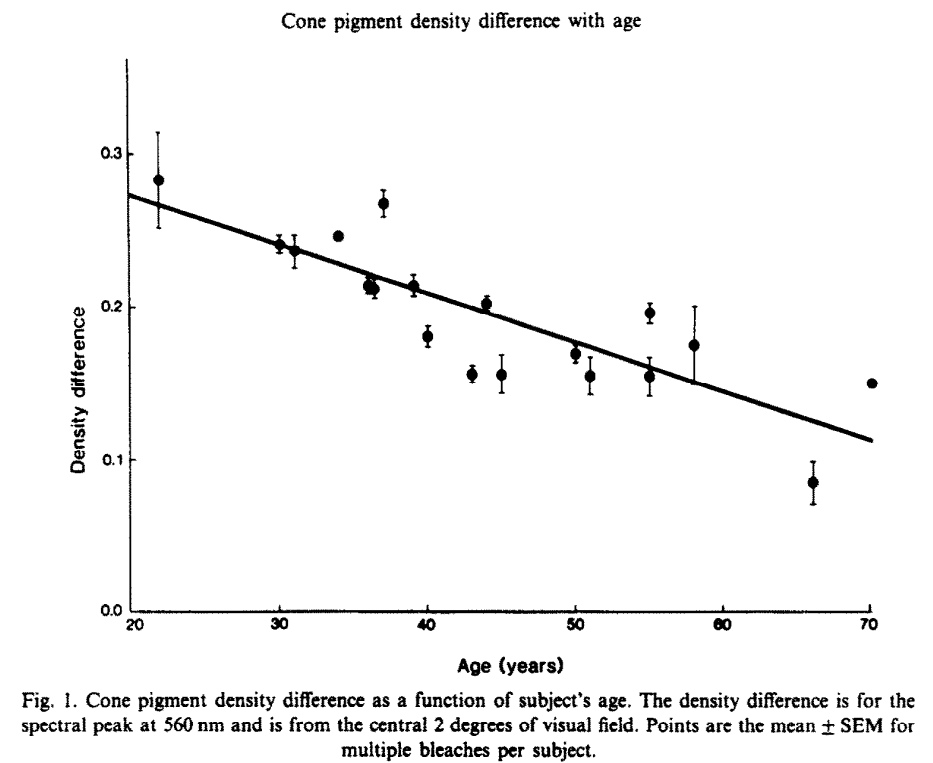
\includegraphics[scale=.5]{Figures/ConeDensityAge}
		\caption{Densité des cônes en fonction de l'âge (figure tirée de \citep{kilbride_foveal_1986})}
		\label{fig:densite_cones_age}
	\end{figure}
	
	\par En conclusion, 
	%\part{Première approche: modèles de vision}
\part{Modèles de vision en Réalité Virtuelle}
	\chapter*{Introduction}
	\addcontentsline{toc}{chapter}{Introduction}
	\markboth{INTRODUCTION}{}
	\par Le terme <<~modèle de vision~>> est très générique et représente en fait un assemblage de briques élémentaires, modulables en fonction des applications et de la finesse du modèle recherchée. Définitions possibles:
	\begin{itemize}
		\item \citep{moreau_traite_2006}: <<~Algorithme qui prend en entrée une image et qui renvoie l'interprétation qu'en fait le système visuel humain.~>>
		\item \citep{pattanaik_multiscale_1998}: <<~Les modèles de vision ont pour objectif de relier la perception visuelle d'un observateur virtuel à la perception visuelle d'un sujet réel regardant un dispositif d'affichage. Le but final étant de caractériser la correspondance visuelle entre la scène virtuelle et l'affichage réel.~>>
	\end{itemize}
	
	\par Un modèle de vision est donc une construction théorique qui vise à reproduire et prédire le fonctionnement de la vision humaine. Le modèle va ainsi intégrer tout un système de modélisation du passage de la lumière dans l'œil, de la captation par la rétine puis du traitement de la lumière par le cerveau. Le modèle de vision est à différencier du prédicateur de vision en cela que ce dernier est inclus, avec d'autres sous-modèles, dans le modèle de vision. Un modèle de vision peut notamment aussi intégrer une prédiction des effets de l'âge mais aussi des comportements plus spécifiques comme le mécanisme d'attention visuelle, ou la reproduction de tons.
	
	\par Nous allons maintenant présenter dans les sections suivantes un état de l'art partiel des modèles de vision, prédicateurs de vision et modèles de reproduction de tons, puis détailler deux modèles particulièrement intéressants:
	\begin{itemize}
		\item Modèle de vision avec vieillissement du système optique \citep{mantiuk_human_2015}.
		\item Prédicateur de vision chromatique complet \citep{pattanaik_multiscale_1998}.
	\end{itemize}
	
	\chapter{État de l'art}
	\par L'état de l'Art ici présenté n'a pas volonté d'être exhaustif sur tous les modèles de vision tant il en existe de types et de variations. On présente néanmoins des classiques ainsi que certaines de leurs ramifications.
	
	\par Si on a défini dans la section précédente le modèle de vision, il reste encore à déterminer les actions et objectifs de deux types de sous-modèles, le Visual Differences Predictor (VDP) et la reproduction de tons:
	\begin{itemize}
		\item La reproduction de tons, ou \textit{tonemapping}, est une technique qui vise à contrebalancer les limites techniques des capteurs d'image par rapport à l'œil humain. En effet, celui ci est -comme on a pu voir précédemment- capable d'intégrer en temps réel un très grand nombre de couleurs et surtout de grands écarts de luminosité, tandis qu'un capteur technologique est (grandement) limité. Le tonemapping est alors une technique pour ramener les informations hors-cadre du capteur dans son champ d'action.
		\item Le VDP est un type d'algorithme qui est amené à donner, objectivement, les différences entre deux traitements d'une même image, par exemple entre l'image initiale et une image après compression. Si le VDP est modélisé sur le système visuel humain, on pourra savoir si les différences entre traitements d'image sont visibles à l'œil nu. Un VDP HDR aura pour objectif de s'assurer que l'interpolation des luminances non-affichables en luminances affichables est efficace.
	\end{itemize}
	
	\par Tout d'abord, il convient de citer les deux modèles fondateurs et sur lesquels la quasi majorité des autres modèles de vision sont adaptés: le \textit{Visual Differences Predictor} de \citep{daly_visible_1992} et le \textit{Visual Discrimination Model} de \citep{lubin_visual_1995}. Si ces deux modèles sont des références absolues, ils restent néanmoins des modèles achromatiques (le traitement et le résultat se font uniquement sur le canal luminance de l'image). Leur équivalent chromatique (traitement sur tous les canaux de l'image, luminance et couleur) est le modèle développé par \citep{pattanaik_multiscale_1998}. Enfin, \citep{rushmeier_comparing_1995} ont formalisé, les premiers, la méthode de reproduction de tons, méthode reprise très largement dans de nombreux modèles par la suite. On en profite également pour pointer vers deux références qui contiennent elle même de très nombreuses références sur le sujet: \citep{moreau_traite_2006} et \citep{bradley_wavelet_1999}.
	
	\section{Modèles principaux dans la littérature}
	\par Le modèle de \citep{daly_visible_1992} est donc un modèle achromatique qui se base sur une simulation de l'adaptation des cellules de la rétine à la luminance. La fonction prend aussi en compte la vision spatiale (c'est à dire la sensibilité aux fréquences spatiales) avec l'intégration de fonctions de sensibilité au contraste. Enfin, le modèle simule aussi les traitement corticaux (c'est à dire la gestion de l'information nerveuse par tout un réseau de neurones) via une fonction dite \textit{cortex}.
		
	\par Parallèlement, le modèle de \citep{lubin_visual_1995} a lui une structure plus logique que le modèle précédent, du point de vue du déroulement de la chaine de vision (de la perception au traitement), néanmoins le traitement se fait toujours de manière achromatique. Il simule l'optique de l'œil et le comportement de la rétine, puis effectue un calcul des contrastes locaux (c'est à dire par zone de l'image perçue) puis il prend en compte l'orientation de l'image et enfin termine par une phase de transduction\footnote{Transducteur. (s.d.). Dans \textit{Dictionnaire Larousse en ligne}. Repéré à \url{http://www.larousse.fr/dictionnaires/francais/transducteur/}}.
	
	\section{Pérennité des modèles principaux}
	\par \citep{lukin_improved_2009} et \citep{bradley_wavelet_1999} ont eu, par rapport au modèle de Daly, des approches radicalement différentes. Le premier a cherché à améliorer la modélisation en complexifiant la fonction de cortex tandis que le second l'a remplacée par une autre approche: une fonction basée sur un modèle en ondelettes.
	Les améliorations de Lukin se concentrent sur une fixation plus précise des seuils utilisés dans la modélisation, l'ajout de la modélisation de l'effet de facilitation pendant l'effet de masque (traitements cognitifs) ainsi que la séparation de l'amplitude et de la phase de la réponse au modèle. L'amplitude servant à calculer le masque de contraste tandis que la phase prend part dans la modélisation de l'effet de facilitation.
	
	\section{Détail des modèles de Mantiuk \textit{et al.}}
	\par Une famille de modèles de vision très intéressante, et basée sur le modèle Daly, est conçue par Rafal Mantiuk et ses collaborateurs: \citep{mantiuk_visible_2004,mantiuk_predicting_2005,mantiuk_human_2015}. Le dernier de ces modèles, qui vient en amélioration des précédents, est d'ailleurs développé en détail par la suite.
	
	\par \citep{mantiuk_visible_2004} proposent un modèle de vision pour les images HDR (High Dynamic Range). Leur hypothèse de base étant que le modèle de Daly est fonctionnel mais reste éloigné de la vision humaine en cela qu'il n'accepte pas une amplitude de luminance suffisante et n'intègre donc pas de mécanisme d'adaptation du système visuel à la luminosité ambiante. Deux modifications principales du modèle initial sont alors opérées:
	\begin{itemize}
	\item Le modèle de Daly part du principe que les photo-récepteurs donnent des réponses égales et subissent des pertes égales quel que soit le niveau de luminance (haut ou bas): une nouvelle transformation de l'information de luminance, cette fois non-linéaire, est proposée.
	\item Une simple fonction de contraste étant insuffisante pour traiter des images avec de grands écarts de luminance, une nouvelle approche est proposée: l'image est filtrée par niveau de luminance puis chaque niveau se voit appliquer une fonction de sensibilité au contraste (CSF).
	\end{itemize}
	
	\par Ensuite, \citep{mantiuk_predicting_2005} apportent une deuxième modification au modèle. La modélisation du passage de la lumière dans l'optique de l'œil est modifiée d'une fonction de diffusion classique (Point Spread Function) au profit d'une fonction de \citep{deeley_simple_1991} (Eq. \ref{eq:deeley_optical_transfer_function}):
	\begin{equation}
	OTF(\rho,d) = \exp \left[ - \left( \frac{\rho}{20.9 - 2.1 \cdot d} \right)^{1.3 - 0.07 \cdot d} \right]
	\label{eq:deeley_optical_transfer_function}
	\end{equation}
	
	\par Avec $\rho$ la fréquence spatiale du stimulus qui traverse l'œil et $d$ le diamètre de la pupille. Ce dernier est quant à lui donné par le modèle de \citep{moon_visual_1944} (Eq. \ref{eq:moon_spencer_pupil_diameter}):
	\begin{equation}
	d = 4.9 - 3 \cdot \tanh \left[ 0.4 \left( \log(Y_{adapt}) + 1.0 \right) \right]
	\label{eq:moon_spencer_pupil_diameter}
	\end{equation}
	
	\par Enfin, \citep{mantiuk_human_2015} apportent une modification fondamentale dans leur modèle, en rajoutant les effets de l'âge de l'observateur simulé sur la perception des erreurs. Ce modèle est largement discuté dans une section suivante (Section \ref{sec:modele_mantiuk}).
	
	\section{Détail des modèles de reproduction de tons}
	\par Après la formalisation de la technique par \citep{rushmeier_comparing_1995}, les algorithmes de reproduction de tons se divisent en trois grandes familles: le traitement des images statiques par des méthodes globales, par des méthodes locales, et le traitement des images dynamiques ; \citep{moreau_traite_2006} relèvent un grand nombre de modèles du genre. Cette dernière famille est entièrement revue par \citep{drago_perceptual_2003}.
	
	\par Enfin, \citep{ferwerda_model_1996} proposent un modèle très complet, basé sur le modèle de reproduction de tons lui-même basé sur le coefficient de Ward que l'on a vu précédemment. Ce modèle fonctionne avec des techniques de calcul d'éclairage plus avancées telle que la \textit{Global Illumination}, et ce, à des niveaux de luminosité allant de photopique à scotopique. Sont modélisés: la capture des changements de seuil de visibilité, les changements d'apparence des couleurs, les changements d'acuité visuelle ainsi que la sensibilité à tous ces facteurs au cours du temps. On peut par exemple obtenir toutes les images intermédiaire d'un processus d'adaptation de l'œil à un changement brutal de luminosité, que ce soit du clair vers l'obscur ou inversement (voir Fig. \ref{fig:ferwerda_adaptation_steps}).
	
	\begin{figure}[h]
		\centering
		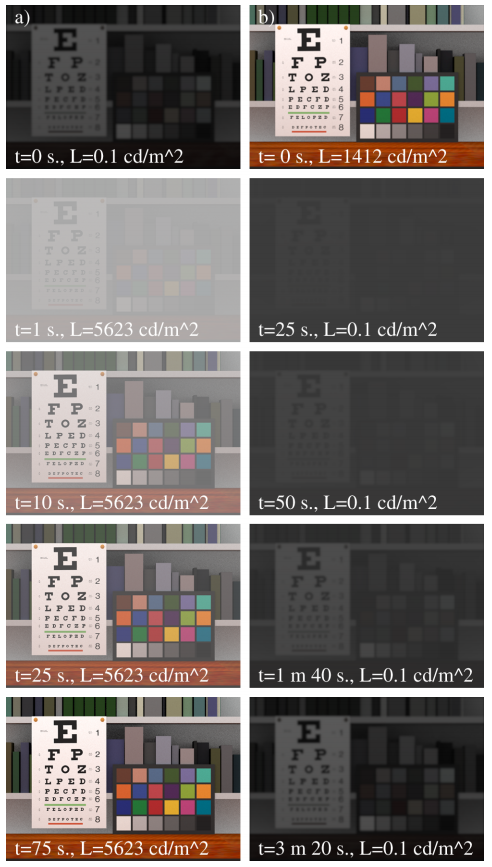
\includegraphics[scale=1]{Figures/FerwerdaAdaptationSteps}
		\caption{Différentes étapes du modèle d'adaptation lumineuse.}{Images tirées de \citep{ferwerda_model_1996}}
		\label{fig:ferwerda_adaptation_steps}
	\end{figure}
	
	\par Nous allons maintenant revenir en détails sur deux modèles particulièrement complets et rigoureux, chacun dans leur domaine: d'un côté le grand mimétisme de la vision humaine et de l'autre la prise en compte avancée des spécificités de l'observateur, et notamment son âge.
	
	\chapter{Modèle de Pattanaik \textit{et al.}}
	\par Le modèle de vision proposé par \citep{pattanaik_multiscale_1998} se positionne face à deux problématiques majeures dans le domaine de l'imagerie informatique: afficher des images ayant un intervalle de luminosité très grand et surtout arriver à afficher des images qui correspondent à une perception similaire à celle de la vision humaine.
	
	\par Il part du principe que beaucoup de modèles ne sont capables de gérer que des informations achromatiques en entrée et font l'impasse sur des caractéristiques plus proches d'une scène naturelle: lumière du jour, amplitude de luminosité étendue, acuité non-uniforme de l'observateur, ...
	
	\par Les auteurs du modèle mettent donc en avant trois points clefs qu'il convient d'utiliser ou d'atteindre dans un modèle de vision:
	\begin{itemize}
	\item des fonctions de sensibilité au contraste (CSFs),
	\item un mécanisme d'adaptation locale de la vision: permet d'améliorer grandement la capacité à voir distinctement dans un intervalle de luminosité très étendu.
	\item un modèle plus élaboré qu'un modèle de seuil: en général, les modèles permettent de définir le seuil en-dessous au au-dessus duquel le visible devient invisible ou inversement. Un modèle plus vaste doit décrire l'intégralité du comportement et non pas uniquement au voisinage du seuil.
	\end{itemize}
	
	\begin{figure}[h]
		\centering
		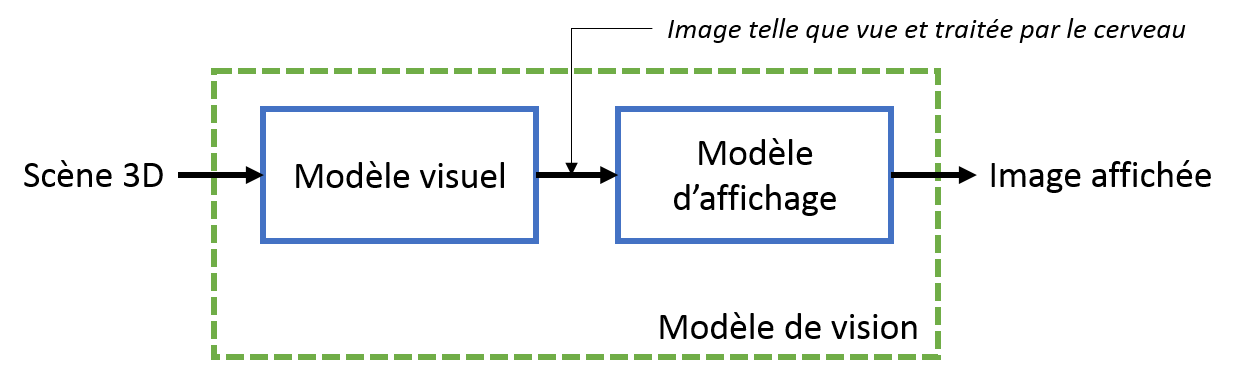
\includegraphics[scale=.75]{Figures/FlowChartPattanaik}
		\caption{Schéma synthétique du déroulé du modèle de \cite{pattanaik_multiscale_1998}}
		\label{fig:flowchart_pattanaik}
	\end{figure}
	
	\par Le modèle proposé est divisé en deux parties principales: le modèle visuel à proprement parler et un modèle d'affichage (voir Fig. \ref{fig:flowchart_pattanaik}). L'algorithme visuel travaille une image d'entrée afin d'en extraire les contrastes des canaux chromatiques et achromatique. Enfin, l'algorithme d'affichage reconstruit une image afin de l'afficher.
	
	\par Le modèle emprunte ses composantes à de nombreux auteurs différents. Il se déroule comme suit (voir Fig. \ref{fig:full_model_pattanaik}):
	\begin{itemize}
		\item Décomposition de l'image via des filtres Gaussiens
		\item Compensation de la dispersion optique dans l'œil, modèle de \citep{westheimer_eye_1986}
		\item Compensation de l'éblouissement, modèle de \citep{spencer_physically-based_1995}
		\item Échantillonnage spectral de tous les étages de la pyramide sauf le plus bas \citep{fairchild_color_1998,wyszecki_color_2000}
		\item Calibration des signaux d'entrée
		\item Traitement spatial des images de chaque canal \citep{burt_laplacian_1983, peli_contrast_1990}
		\item Conversion en canaux chromatiques et achromatique (théorie des processus antagoniques) \citep{hunt_reproduction_1995,fairchild_color_1998}
		\item Passage par des transducteurs de contraste \citep{watson_model_1997}
		\item Combinaison des signaux des cônes et des bâtonnets
		\item Traitement de l'étage de la pyramide restant (le plus bas, qui a été laissé de côté dans la quatrième étape) \citep{fairchild_color_1998}
		\item Résultats du modèle visuel
		\item Reconstruction de l'image par traitement inversé pour l'affichage
	\end{itemize}
	
	\par L'image doit être décomposée à l'aide de filtres gaussiens, de telle manière à ce que les bandes-passantes (ce qui est gardé dans le filtre) correspondent à des fréquences spatiales bien définies: $16$, $8$, $4$, $2$, $1$ et $0.5~cpd$\footnote{cpd: cycles par degrés.}.
	
	\par On réalise ensuite un échantillonnage spectral dans le but de reproduire la réponse des différents cônes et bâtonnets présents dans la rétine. Cet échantillonnage se fait par l'intégration de la distribution de radiance pour chaque pixel après multiplication par l'efficacité lumineuse des photo-récepteurs mis en jeu. L'efficacité pour les cônes est donnée par les courbes de Hunt, Pointer et Estevez \citep{fairchild_color_1998} tandis que l'efficacité des bâtonnets est donnée par l'observateur scotopique de la CIE \citep{wyszecki_color_2000}.
	
	\par Cependant, dans la majeure partie des cas, la valeur de radiance du pixel n'est pas disponible et doit être calculée pour les cônes par une transformation linéaire depuis les valeurs du tri-stimulus CIE 1931 XYZ (Eq. \ref{eq:pattanaik_linear_transform_cones_signal}). Pour les bâtonnets, une approximation est nécessaire, en utilisant l'Eq. \ref{eq:pattanaik_approximation_rods_signal}:
	\begin{equation}
		\left[ \begin{array}{c}L\\ M\\ S\end{array} \right] = \left[ \begin{array}{ccc}
		0.3897 & 0.6890 & -0.0787\\
		-0.2298 & 1.1834 & 0.0464\\
		0 & 0 & 1		
		\end{array} \right] \times \left[ \begin{array}{c}X\\ Y\\ Z\end{array} \right]
		\label{eq:pattanaik_linear_transform_cones_signal}
	\end{equation}
	
	\begin{equation}
		R = -0.702 \cdot X + 1.039 \cdot Y + 0.433 \cdot Z
		\label{eq:pattanaik_approximation_rods_signal}
	\end{equation}
	
	\par Les différents canaux sont ensuite soumis à un traitement spatial, une décomposition en pyramide laplacienne de 7 étages \citep{burt_laplacian_1983}. Les 6 premiers étages sont ensuite convertis en images contrastées \citep{peli_contrast_1990} au moyen d'un gain de luminance (Eq. \ref{eq:pattanaik_laplacian_pyramid_equations}):
	\begin{equation}
		\begin{array}{c}
		G_{cone}(I) = \frac{1}{0.555 \cdot (I+1.0)^{0.85}}\\
		G_{rod}(I) = \left[ \frac{10}{I^2+10} \right] \times \left[ \frac{1}{0.908 \cdot (I+0.001)^{0.85}} \right]
		\end{array}
		\label{eq:pattanaik_laplacian_pyramid_equations}
	\end{equation}
	On obtient au final une image au contraste adapté pour un certain niveau ($ACI_n$ - Image avec contraste adapté au niveau $n$), avec $LP_n$ la réponse au filtre passe-bas de l'image de niveau $n$ ($n$ allant de 1 à 6, en fonction de l'étage de la pyramide concerné) (Eq. \ref{eq:pattanaik_peli_adapted_contrast}):
	\begin{equation}
		ACI_n = G(LP_{n+1}) \times \left[ LP_n - LP_{n+1} \right]
		\label{eq:pattanaik_peli_adapted_contrast}
	\end{equation}
	
	\par Les images contrastées obtenues juste avant, sont ensuite transformées encore, jusqu'au système $AC_1C_2$ qui reprend la théorie des processus antagoniques, c'est à dire le découpage du traitement de l'image par le cerveau en un canal achromatique ($A$), et deux canaux chromatiques ($C_1$ et $C_2$), voir sections précédentes sur la couleur. La transformation se fait au moyen d'une banale matrice de passage \citep{hunt_reproduction_1995,fairchild_color_1998}:
	\begin{equation}
		\left[ \begin{array}{c}A\\ C_1\\ C_2\end{array} \right] = \left[ \begin{array}{ccc}
		2.0 & 1.0 & 0.05\\
		1.0 & -1.09 & 0.09\\
		0.11 & 0.11 & -0.22		
		\end{array} \right] \times \left[ \begin{array}{c}L\\ M\\ S\end{array} \right]
		\label{eq:pattanaik_linear_transform_lms_to_ac1c2}
	\end{equation}
	
	\par Le signal passe en suite à travers des transducteurs basés sur le contraste pour reproduire la sensibilité au contraste de l'œil. Pour rappel, un transducteur\footnote{Transducteur. (s.d.). Dans \textit{Dictionnaire Larousse en ligne}. Repéré à \url{http://www.larousse.fr/dictionnaires/francais/transducteur/}} est une fonction ou un mécanisme qui permet de transformer une grandeur en une autre, comme par exemple un mouvement en électricité ou une lumière en électricité. Les transducteurs sont ici utilisés pour supprimer de l'image le contraste qui serait imperceptible dans les conditions (d'éclairage) données. Leurs valeurs sont limitées à 50 pour reproduire les limitations en luminosité du système visuel. Les auteurs du modèle utilisent les équations de \citep{watson_model_1997} modifiées pour être inversibles (Eq. \ref{eq:pattanaik_transducers}):
	\begin{equation}
	\begin{array}{c}
	
	T_{cone,achromatic}(c) = \begin{cases}
	22.4 \cdot \sqrt{\frac{c}{0.536}} & \mbox{si } c \geq 0.536\\
	22.4 \cdot \left( \frac{c}{0.536} \right)^p & sinon
	\end{cases}\\
	
	T_{cone,chromatic}(c) = \begin{cases}
	22.4 \cdot \sqrt{\frac{c}{0.176}} & \mbox{si } c \geq 0.176\\
	22.4 \cdot \left( \frac{c}{0.176} \right)^p & sinon
	\end{cases}\\
	
	T_{rod}(c) = \begin{cases}
	22.4 \cdot \sqrt{\frac{c}{0.0335}} & \mbox{si } c \geq 0.0335\\
	22.4 \cdot \left( \frac{c}{0.0335} \right)^p & sinon
	\end{cases}
	
	\end{array}
	\label{eq:pattanaik_transducers}
	\end{equation}
	
	\par Les valeurs de p sont données dans la Tab. \ref{tab:pattanaik_transducers_p_values}.
	
	\begin{table}
		\centering
		\label{tab:pattanaik_transducers_p_values}
		\small
		\begin{tabular}{|l|l|l|l|l|l|l|}
			\hline
			\textbf{Fréquence spatiale (cpd)} & \textbf{0.5} & \textbf{1.0} & \textbf{2.0} & \textbf{4.0} & \textbf{8.0} & \textbf{16.0}\\
			\hline
			\hline	
			\textbf{p (achromatique)} & 1.93 & 1.35 & 1.15 & 1.04 & 1.15 & 1.40\\
			\hline
			\textbf{p (chromatique)} & 1.93 & 1.93 & 2.35 & 2.85 & - & -\\
			\hline
			\textbf{p (bâtonnets)} & 3.39 & 3.39 & 4.50 & 7.64 & - & -\\
			\hline
		\end{tabular}
		\caption{Valeurs de la puissance dans les fonctions de transducteurs de \cite{watson_model_1997}}
	\end{table}
	
	\par Le canal chromatique final est en fait une combinaison des valeurs de la composante A des tri-stimulus des cônes et des bâtonnets. Le calcul se fait au moyen de l'Eq. \ref{eq:pattanaik_combination_rodes_cones}. La valeur $7$ est obtenue par calibration:
	\begin{equation}
		A_{total} = A_{cones} + \frac{A_{batonnets}}{7}
		\label{eq:pattanaik_combination_rodes_cones}
	\end{equation}
	
	\par Cette étape conclut le traitement des 6 premiers étages de la pyramide de décomposition.
	
	\par Après quoi, le traitement du dernier et septième étage de la pyramide se fait via des transducteurs passe bas (Eq. \ref{eq:pattanaik_lowpass_transducers}) \citep{fairchild_color_1998}:
	\begin{equation}
		\begin{cases}
			T_{LP,cones,achromatique}(LP) = 30.5 \cdot \sqrt{LP}\\
			T_{LP,cones,chromatique}(LP) = 53.3 \cdot \sqrt{LP}\\
			T_{LP,batonnets}(LP) = 122 \cdot \sqrt{LP}\\
		\end{cases}
		\label{eq:pattanaik_lowpass_transducers}
	\end{equation}
	
	\par Au point intermédiaire, à l'issue du modèle visuel, on obtient donc les résultats suivants:
	\begin{itemize}
		\item 1 canal achromatique
		\item 2 canaux chromatiques
		\item 6 images issues d'un filtre spatial bande-passante
		\item 1 image issue d'un filtre passe-bas
	\end{itemize}
	
	\par Enfin, on effectue le processus de reconstruction de l'image en faisant un traitement étape-par-étape inverse par rapport au modèle visuel de manière à recréer le signal perçu par les cônes pour l'afficher. On prend les fonctions inverses des transducteurs évoqués précédemment (Eq. \ref{eq:pattanaik_lowpass_transducers}). On passe d'une décomposition de la lumière en mode chromatique/achromatique ($AC_1C_2$) au découpage reproduisant le fonctionnement des bâtonnets et cônes ($LMS$), en utilisant la matrice inverse et enfin on applique un mécanisme de gain inverse en fonction des conditions d'affichage. Pour finir, on effectue la dernière transformation en allant de $LMS$ à l'espace colorimétrique adapté au moyen d'affichage (CIECAM, CIELAB, CIELUV, RGB, ...).
	
	\begin{figure}[h]
		\centering
		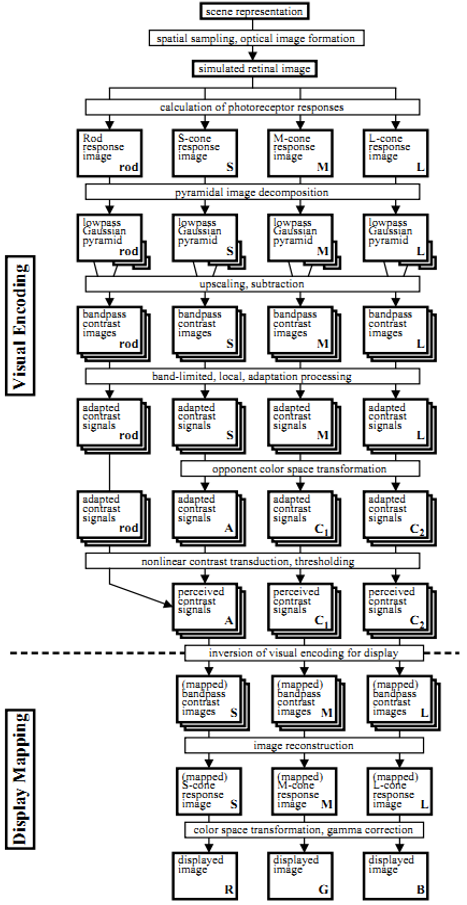
\includegraphics[scale=1.25]{Figures/PattanaikFullModel}
		\caption{Schéma exhaustif du traitement de l'image par le modèle de \cite{pattanaik_multiscale_1998}}
		\label{fig:full_model_pattanaik}
	\end{figure}
	
	\par En conclusion, \citep{pattanaik_multiscale_1998} ont mis sur pied un modèle extrêmement précis et pertinent, composé de sous-modèles disponibles dans la littérature. Cependant, ce modèle est statique, c'est à dire qu'il ne prend pas en compte la composante temporelle et ne fonctionne que pour traiter une image seule, et non pas intégré dans une boucle de calcul d'image en temps réel. Nous allons maintenant aborder le modèle de \citep{mantiuk_human_2015}.
	
	\chapter{Modèle de Mantiuk \& Ramponi}
	\label{sec:modele_mantiuk}
	\par Comme on a pu voir précédemment, l'âge de l'observateur peut avoir une grande influence sur un certain nombre de paramètres dans la vision ; tant de manière physiologique que cognitive. Cependant, le modèle que nous présentons ici, celui de \citep{mantiuk_human_2015}, est basé sur un prédicateur nommé HDR-VDP-2 et amélioré selon quatre grands axes: le vieillissement du cristallin, la réduction du diamètre de la pupille avec l'âge, les éblouissement invalidants et une composante de dégradation cognitive. 
	
	\par La contribution la plus importante à la dégradation de la vision au cours du temps vient du vieillissement du cristallin. La lentille continue de grossir et de générer des nouvelles fibres, compressant et accumulant ainsi les fibres plus anciennes dans la région centrale du cristallin. Celui-ci devient donc de plus en plus rigide et de moins en moins transparent.
	
	\par Le cristallin est modélisé comme un filtre optique dépendant de la longueur d'onde et qui réduit la quantité de lumière que la rétine reçoit. Cependant ce filtre a peu d'effet en vision photopique (vision de jour) et est plus efficace en dessous de $3~cd/m^2$, c'est à dire dans les domaines mésopique et scotopique.
	\citep{mantiuk_human_2015} reprennent ici le modèle de \citep{pokorny_aging_1987}. pour le vieillissement du cristallin (Eq. \ref{eq:vieillissement_cristallin}):
	\begin{equation}
		O_D(a) = \begin{cases}
			 L_1 \cdot (1+0.02 \cdot (a-32))+L_2 & a \leq 60 \\ L_1 \cdot (1.56+0.0667 \cdot (a-60))+L_2 & a \geq 60 \end{cases}
		\label{eq:vieillissement_cristallin}
	\end{equation}
	
	\par Avec $O_D$ la densité optique du cristallin, $a$ l'âge du sujet et $L_1$, $L_2$ des constantes issues de tables dans le modèle de Porkony \textit{et al.}.
	
	
	\par \citep{mantiuk_human_2015} incluent aussi dans leur modèle un mécanisme d'efficacité lumineuse (valable seulement dans le domaine photopique) qui fut validé et entériné par la CIE en 1924. Les résultats liés à ce modèle sont disponibles chez \citep{sagawa_spectral_2001}.
	
	\par L'éblouissement (ou \textit{Sensibility Glare} en anglais) est une pollution lumineuse qui intervient en présence de lumière très vive directement dans le champ de vision. Cette pollution atténue les hautes fréquences spatiales et réduit le contraste perçu sur la rétine. La prise en compte de la sensibilité à l'éblouissement en fonction de l'âge est elle aussi étayée par un modèle de la CIE: \citep{vos_cie_1999}.
	
	\par Le diamètre pupillaire moyen tend à diminuer avec l'âge, on parle alors de \textit{myosis} (l'effet contraire étant la \textit{mydriase}). Ce phénomène a été modélisé par un grand nombre de chercheurs différents ; \citep{watson_unified_2012} proposent à la fois une revue des différents modèles mais surtout un modèle unifié pour l'évolution du diamètre de la pupille. C'est ce modèle qui est utilisé dans le modèle de vision avec vieillissement de l'œil de \citep{mantiuk_human_2015}.
	
	\par Le modèle est le suivant (Eq. \ref{eq:diam_pupille_aging}):
	\begin{equation}
		\begin{cases}
		S(l,a,f) = (a-28.58) \times (0.02132-0.009562 \cdot D_{SD})\\
		D_{SD} = 7.75 - \frac{5.75 \times k}{k+2}\\
		k = \left( \frac{L \times f}{846} \right)^{0.41}
		\end{cases}
		\label{eq:diam_pupille_aging}
	\end{equation}
	
	\par Avec $S$ le diamètre pupillaire, $a$ l'âge de l'individu, $L$ le niveau de luminosité auquel l'œil est adapté (en $cd/m^2$) et $f$ la zone de champ.
	
	\par Ensuite, \citep{burton_aging_1993} ont mesuré la perte de sensibilité causée par l'affectation des récepteurs et des processus cognitifs entre des jeunes adultes et des personnes âgées. Ces mesures ont été réalisées avec un laser permettant d'ignorer le système optique et d'envoyer directement une image sur la rétine. Les résultats donnent de légères variations entre les populations d'âge différent. \citep{mantiuk_human_2015} proposent alors leur propre modèle empirique (Eq. \ref{eq:neural_component_model_mantiuk}):
	\begin{equation}
		log_{10}(\Delta S) = - (\beta \times log_2(\rho + a)) \times max(a-24;0)
		\label{eq:neural_component_model_mantiuk}
	\end{equation}
	
	\par Avec $a$ l'âge du sujet, $\rho$ la fréquence spatiale du stimulus (en $cpd$). $\alpha = 0.75$ et $\beta = 0.00195$ sont des valeurs empiriques proposées par les auteurs du modèle.
	
	\par Enfin, cette modélisation est toutefois à prendre avec recul car un grand nombre de valeurs utilisées ici ont été mesurées pendant des expérimentations réalisées sur des écrans CRT (Cathodiques) ayant un spectre de luminosité assez réduit (de $0.1$ à $80~cd/m^2$).
	
	\chapter*{Conclusion}
	\addcontentsline{toc}{chapter}{Conclusion}
	\markboth{CONCLUSION}{}
	\par L'étude des modèles de visions et leurs traductions vers le domaine de l'informatique semble être un domaine déjà fortement décrit et bien maitrisé. Une contribution directe dans ce domaine n'est alors ni très évidente ni très pertinente. On pourrait éventuellement tenter d'appliquer le modèle de Pattanaik \textit{et al.} en temps réel mais la portée scientifique semble limitée. On décide alors de laisser cette approche de côté pour en prendre une nouvelle.
	
	\par Plutôt que de s'intéresser à une capture d'image respectant le même processus que la vision humaine, on se penche sur un autre aspect jouant un rôle prépondérant dans le réalisme: l'affichage correct de ce qui a été capturé dans la scène 3D. En effet, si une fois l'image capturée proprement (via une mise en place du modèle de Pattanaik \textit{et al.} par exemple) le système n'est pas capable de restituer l'image dans la même gamme de perception que celle de l'œil humain, le réalisme vis à vis de l'utilisateur en sera amoindri.
	
	\par On propose alors, non pas de développer un modèle d'affichage, mais une méthode pour quantifier la qualité du système d'affichage immersif, en fonction de la modélisation du système visuel humain.
	\part{Deuxième approche: score de réalisme}
	\chapter*{Introduction}
	\addcontentsline{toc}{chapter}{Introduction}
	\markboth{INTRODUCTION}{}
	\par Pour rappel, on avait posé dans la définition du réalisme (\textit{cf.} Chapitre \ref{part:edla}.\ref{chap:def_realisme}) le cadre d'étude suivant:
	\begin{quote}
		<<~Pour le cas de cette thèse, la définition du réalisme qui aura été retenue -et qui sera sous-entendue quand on utilisera le mot \textit{réalisme} seul- est celle de la proximité physiologique avec le système visuel humain. [...] Le réalisme physiologique doit, par construction et par définition, se baser sur le système visuel humain.~>>
	\end{quote}
	La première approche, qui était de développer un <<~modèle de vision~>> traduit pour la Réalité Virtuelle et les caméras qui extraient les images des scènes 3D, s'est vite révélée être une impasse ou en tout cas une voie offrant peu de débouchés tant ces modèles étaient déjà largement décrits dans la littérature.
	
	\par On choisit alors une approche différente: plutôt que de \textit{faire} du réalisme, il pourrait être intéressant de \textit{quantifier} le réalisme qu'un-e système/application produit. En effet, si on entend souvent parler de réalisme, son appréciation est souvent binaire: soit un système ou une application est réaliste, soit il/elle ne l'est pas. De plus, il est difficile de pouvoir dire concrètement ce qui rend un système moins réaliste qu'un autre. Pour ce faire, il faudrait pouvoir être capable de mettre des valeurs et des critères objectifs à remplir. On aurait alors un moyen efficace et juste de juger du réalisme d'un système et/ou de comparaison entre plusieurs éléments.
	
	\par Outre sa dimension théorique, on anticipe deux usages potentiels à une telle approche: elle pourrait permettre de choisir un système pour un cas d'usage donné. En fonction des critères dont on a besoin principalement, on pourra se référer aux notes pour faire un choix. De même, le système de notation permettrait de comparer les dispositifs immersifs et ainsi de les positionner entre eux.
		\part{Deuxième approche: score de réalisme} \newpage
	\chapter*{Introduction}
	\addcontentsline{toc}{chapter}{Introduction}
	\markboth{INTRODUCTION}{}
	\par Pour rappel, on avait posé dans la définition du réalisme (\textit{cf.} Chapitre \ref{part:edla}.\ref{chap:def_realisme}) le cadre d'étude suivant:
	\begin{quote}
		<<~Pour le cas de cette thèse, la définition du réalisme qui aura été retenue -et qui sera sous-entendue quand on utilisera le mot \textit{réalisme} seul- est celle de la proximité physiologique avec le système visuel humain. [...] Le réalisme physiologique doit, par construction et par définition, se baser sur le système visuel humain.~>>
	\end{quote}
	La première approche, qui était de développer un "modèle de vision" traduit pour la Réalité Virtuelle et les caméras qui extraient les images des scènes 3D, s'est vite révélée être une impasse ou en tout cas une voie offrant peu de débouchés tant ces modèles étaient déjà largement décrits dans la littérature.
	
	\par On choisit alors une approche différente: plutôt que de "faire" du réalisme, il pourrait être intéressant de "quantifier" le réalisme qu'un-e système/application fait. En effet, si on entend souvent parler de réalisme, son appréciation est souvent binaire: soit un système ou une application est réaliste, soit il/elle ne l'est pas. De plus, il est difficile de pouvoir dire concrètement ce qui rend un système moins réaliste qu'un autre. Pour ce faire, il faudrait pouvoir être capable de mettre des valeurs et des critères objectifs à remplir. On aurait alors un moyen efficace et juste de juger du réalisme d'un système et/ou de comparaison entre plusieurs éléments.
	
	\par A notre connaissance, il existe peu voire très peu de modèles ayant pour but de quantifier objectivement le réalisme physiologique dans la littérature. Ce type de modèle ne doit pas être confondu avec les méthodes de qualifications de la qualité de l'image qui elles sont basées sur une comparaison entre une image source et cette même image après qu'elle soit passée à travers tout un processus de transformation (comme par exemple, un encodage vidéo) \citep{cadik_human_2004, winkler_quality_2000} (\textit{cf.} Figure \ref{fig:quality_process}). Actuellement, il existe déjà un grand nombre de méthodes pour la qualité d'image, notamment pour des images 2D (images statiques ou vidéos). Ces dernières années, l'accent à plutôt été mis sur le développement de techniques de qualification de la qualité pour des images 3D. On peut trouver un certain nombre de review de ces techniques dans la littérature \citep{moorthy_subjective_2013, moorthy_survey_2013} voire même avec une dimension subjective en plus \citep{beghdadi_survey_2013}.
	
	\begin{figure}
		\centering
		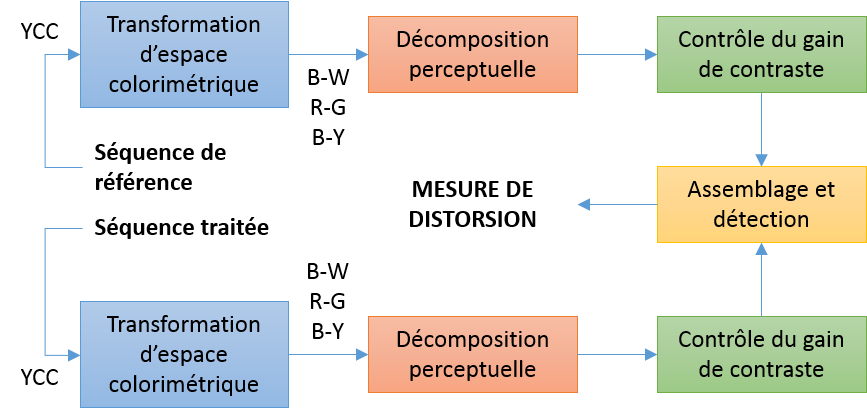
\includegraphics[scale=1]{Figures/ImageQualityWinkler}
		\caption{Fonctionnement du processus de mesure de qualité d'image, pour des séquences vidéo 2D. Traduction d'une figure reprise de \cite{winkler_quality_2000}}
		\label{fig:quality_process}
	\end{figure}
	
	\par Le réalisme en tant que tel est quant à lui en général plutôt mesuré par une question directe sur le réalisme de l'expérience à laquelle le sujet vient de participer (ce qui est à relier avec la quatrième acceptation du réalisme, le réalisme \textit{psychologique} et non pas le réalisme \textit{physiologique}). Des approches plus détaillées peuvent se servir de questionnaires \citep{fucentese_evaluation_2015, fiard_initial_2014}.
	
	\par Néanmoins, on trouve quelques approches objectives pour la définition du réalisme bien que ce ne soit pas forcément leur objectif principal:	
		\begin{itemize}
			\item Le modèle de Rose \citep{rose_sensitivity_1948,burgess_rose_1999}.
			\item Le modèle d'observateur idéal \citep{geisler_ideal_2003}.
		\end{itemize}
		
		\section*{Modèle de Rose}		
		\par Le modèle de Rose est une première tentative (à l'époque pour la télévision en noir et blanc !) de caractérisation de "l'enregistreur d'image" idéal, vis à vis de la vision humaine. Le modèle est conçu pour la capture d'un objet unique, c'est à dire que le modèle donne les caractéristiques qu'un objet unique doit avoir pour être capturé par l'enregistreur idéal. On peut le décrire par l'équation  suivante (Eq. \ref{eq:modèle_rose}), avec $B$ la luminance de l'objet en footLamberts\footnote{NB: $1~fL \approx 3.426~cd/m^2$}, $C$ le contraste de l'objet comparé au background (en pourcentage) et $\alpha$ l'angle de visuel sous lequel l'objet est vu par l'enregistreur.
		
		\begin{equation}
			BC^2\alpha^2 = \text{constant}
			\label{eq:modèle_rose} 
		\end{equation}
		
		\section*{Observateur idéal \& théorie de détection du signal}		
		\par La définition d'un "observateur idéal" est basée sur une théorie appelée "détection du signal" (Signal Dedection Theory). Cette théorie décrit la capabilité d'un système à discerner un pattern spécifique au milieu d'autres patterns ou bien au milieu d'un bruit (cf. Fig. \ref{fig:signal_detection_theory}). Le théorie de détection du signal est également basée sur la théorie bayésienne qui est l'interprétation du concept de probabilités comme état de savoir -le pattern est visible ou non- plutôt qu'une fréquence ou une propension d'apparition d'un phénomène. La théorie de détection du signal inclue également des probabilités de détection et des seuils de vision. Cependant, les observateurs idéaux sont utilisés pour une unique tâche bien spécifique (au contraire de la vision que se veut généraliste) telle que la détection de photon, la détection de pattern, l'identification ...
		
		\begin{figure}
			\centering
			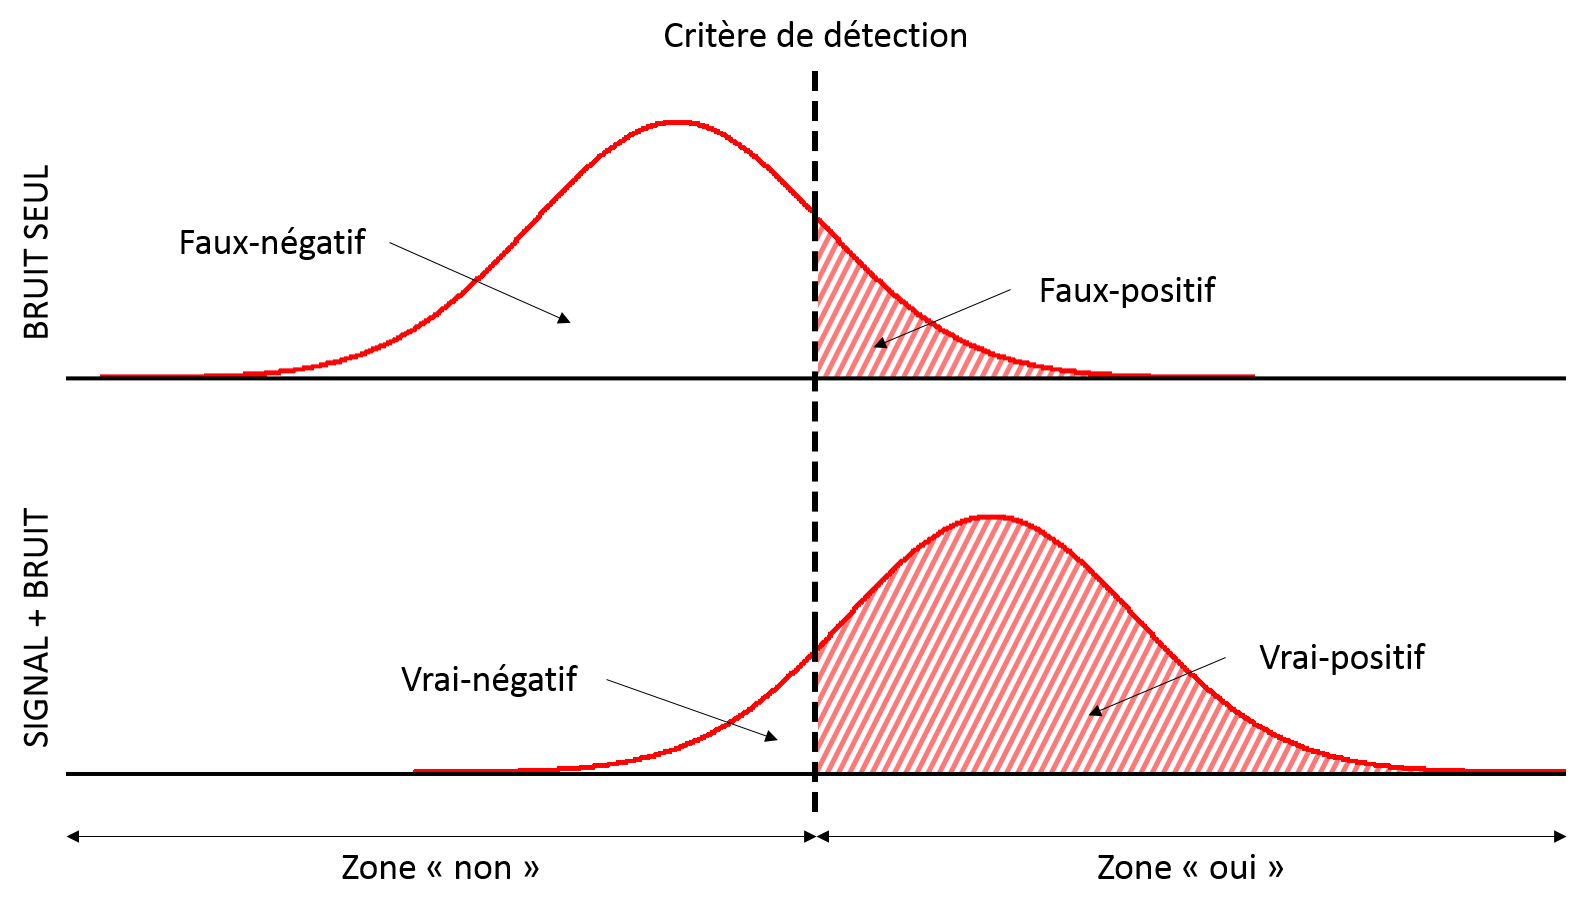
\includegraphics[scale=.5]{Figures/SignalDetectionTheory}
			\caption{Illustration de la théorie de détection du signal. Répartition des probabilités de détection autour d'un seuil de détection déterminé (critère de détection)}
			\label{fig:signal_detection_theory}
		\end{figure}
	
	\chapter{Score de réalisme}
	\section{Ambition}	
	\par On a vu dans les modèles présenté précédemment dans l'introduction, et notamment dans celui de Rose qui mêle dans une équation mathématique simple des grandeurs essentielles pour le réalisme (contraste, luminance, taille), une approche pragmatique de la définition du réalisme physiologique. Néanmoins, il manque toujours une dimension à ces modèles: les modèles de Rose et d'observateur idéal prédisent pour l'un les qualités optimales d'affichage et pour l'autre la moment à partir duquel l'œil humain va percevoir l'objet puis une description de la probabilité de plus en plus élevée de le percevoir, mais jamais les deux en même temps.
	
	\par Au delà de ces modèles, on souhaite être capable de pouvoir quantifier le biais qu'il existe entre ce qui est affiché dans un environnement virtuel et la qualité de perception de l'utilisateur. C'est à dire non seulement être capable de dire quelles sont les conditions optimales pour que le système visuel humain interagisse avec l'affichage immersif mais aussi pouvoir apprécier les conditions non-optimales, tel que le système de probabilité dans le modèle d'observateur idéal. On souhaite néanmoins réfléchir à une autre approche que celle probabiliste pour se rapprocher d'un démarche plus pragmatique, plus <<ingénieur>>.
	
	\par Cette méthode pourrait alors indiquer à quel point l'interaction entre le système visuel humain et l'affichage est différente de l'interaction qui aurait lieu dans le monde naturel et ce de manière tangible, mesurée. Pour que l'évaluation soit fiable et répétable, la quantification doit être complètement objective et doit dépendre de critères physiques du système d'affichage (hardware).
	
	\par On propose alors une évaluation de la performance d'un système via un score qui dépeindrait, pour un système immersif donné et pour une situation donnée, à quel point le simulateur est efficace pour transmettre le bon niveau d'informations visuelles et, étant dans un système de Réalité Virtuelle, le bon niveau d'indices d'immersion.
	
	\begin{figure}
		\centering
		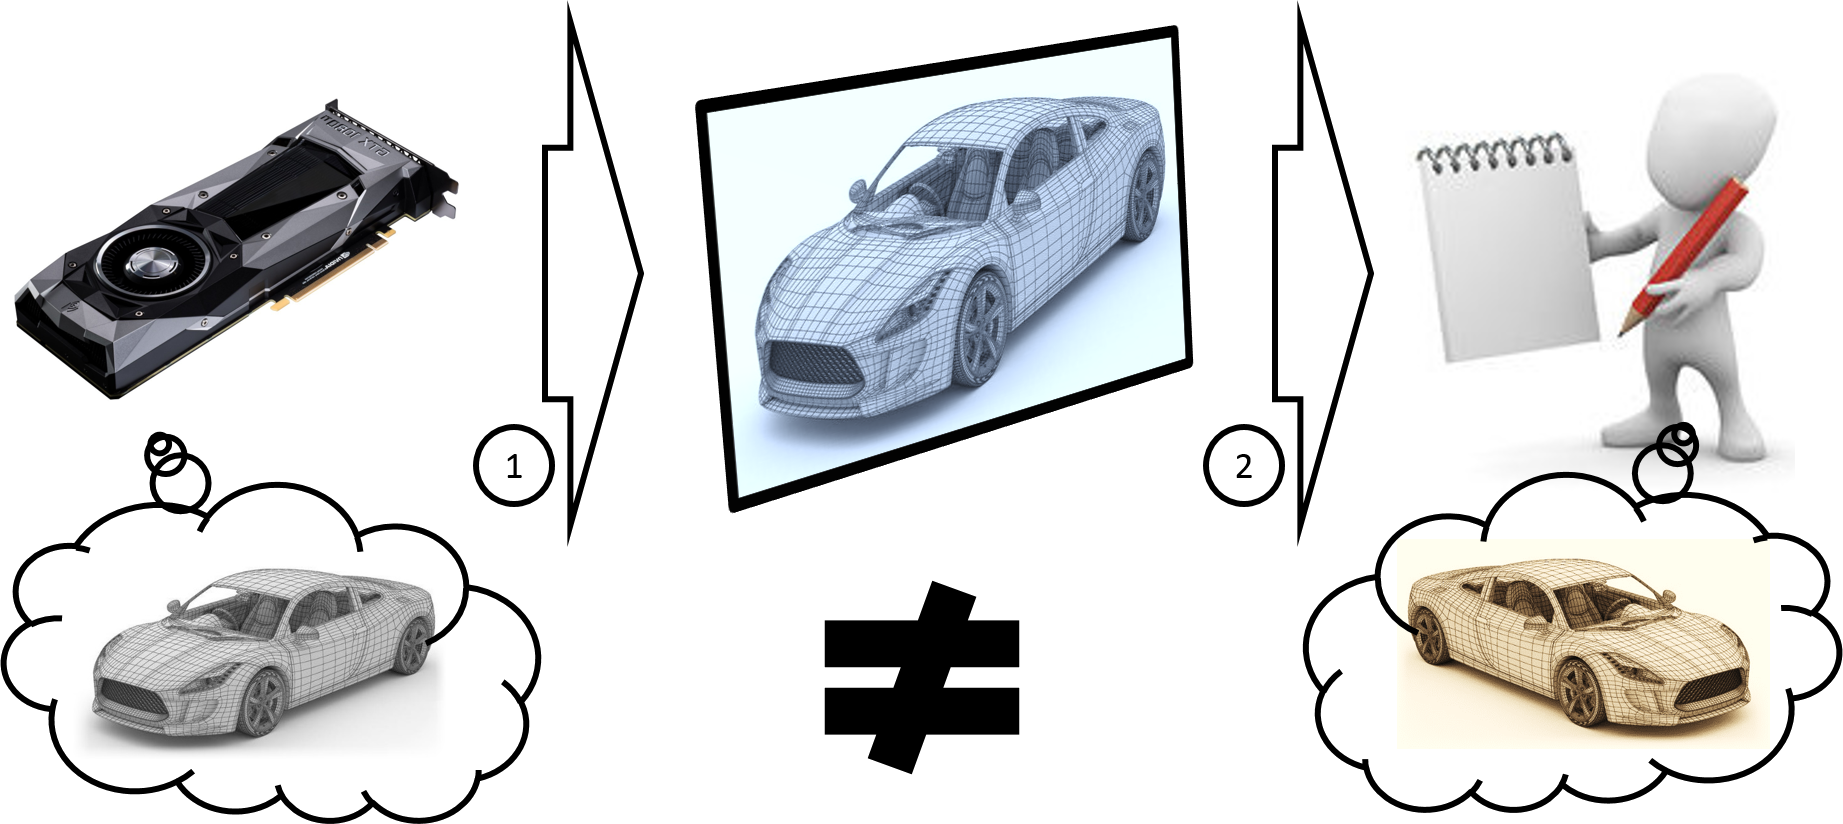
\includegraphics[scale=.45]{Figures/ImageBias}
		\caption{Illustration de la différence qu'il existe entre les consignes données par la carte graphique (1) et les informations visuelles reçues par l'observateur (2).}
		\label{fig:image_bias}
	\end{figure}
			
	\section{Méthodologie}
	\par On propose donc un système de score qui serait basé sur le système visuel humain. Ce score est en fait la réunion d'un certain nombre (à définir, voir par la suite) de sous-scores chacun lié à une caractéristique de la vision et/ou de l'immersion liée à la vision (c'est à dire les critères immersifs dérivés directement du système visuel ou du système en lui même). Chaque critère est jugé indépendamment puis contribue à la note globale via une pondération.
	
	\par La première étape était donc logiquement d'avoir une connaissance et une compréhension approfondie du système visuel humain. Comme on a pu voir dans la première partie, qui présente cette étude de l'état de l'Art, on s'est intéressé d'abord au fonctionnement de l'œil en lui-même puis de ce qu'il se passe après, que ce soit le traitement nerveux ou le traitement par le cerveau. L'accent à ensuite été mis sur le contraste et la couleur qui sont des deux grandes caractéristiques de l'image ainsi que la perception visuelle de la profondeur. Enfin, certaines influences, classées ici abusivement comme << physiologiques >>, modifient le processus normal de la vision et doivent être, si possible, prises en compte.
	
	\par Deuxièmement, une fois cette connaissance acquise il a fallut découper le processus de vision et les facteurs d'immersions en différents critères. Ce processus à été long et compliqué, et fait l'objet d'un chapitre pour le détailler (voir par la suite). Ces critères se veulent indépendants les uns des autres mais des relations ont quand même parfois été relevées entre certains critères. Par exemple, la précision de la vision dépend dans certains cas de la luminosité: une situation bien éclairée permet de voir bien plus précisément qu'une situation mal éclairée. Pour plus de simplicité et de clarté, on a regroupé les critères par domaine.
	
	\par Troisièmement, une fois les critères établis, il convient de les évaluer. Pour ce faire, on propose d'attribuer une note comprise en 0 et 100 à chacun des critères du modèle. Cette note modélise le fonctionnement du critère en question: le note de 0 représente les conditions dans lesquelles le système de vision n'est pas capable d'utiliser le mécanisme (ou peut l'utiliser mais n'en tire aucune information utile) tandis que la note de 100 représente le fonctionnement ou la performance maximal-e du mécanisme de vision. On rajoute également une note intermédiaire à 80 qui représente le fonctionnement nominal du mécanisme de vision. La valeur de 80 est plus probablement la valeur de score à viser car la valeur de 100 représente la maximum possible de l'œil humain et pourrait être considéré comme de la sur-qualité par rapport à la performance nominale. Il est évident que dans certaines applications, atteindre la valeur de 100 peut être une nécessité. Cette démarche est confortée par le fait que la Commission Internationale pour l'Eclairage (CIE) procède de la même manière (noter sur une valeur de 100 en adjugeant 80 à la valeur nominale) dans son modèle de performance visuelle en fonction de la luminosité et du contraste (voir plus loin la partie spécifique sur la luminance et le contraste). 
	
	\par La notation en elle même se fait, principalement, basée sur la littérature: on cherche les valeurs correspondantes aux fonctionnements minimal, nominal et maximal. On cherche ensuite une loi mathématique simple permettant de décrire l'évolution de la note en fonction des valeurs clefs du mécanisme visuel. Si on a pu appliquer cette méthode pour la majorité des cas, certains critères ne se prêtent pas à un tel traitement et ont bénéficié d'une notation particulière. Cette notation sera explicitée plus bas, au cas par cas, dans la présentation des critères retenus dans la dernière version du modèle.
	
	\begin{figure}
		\centering
		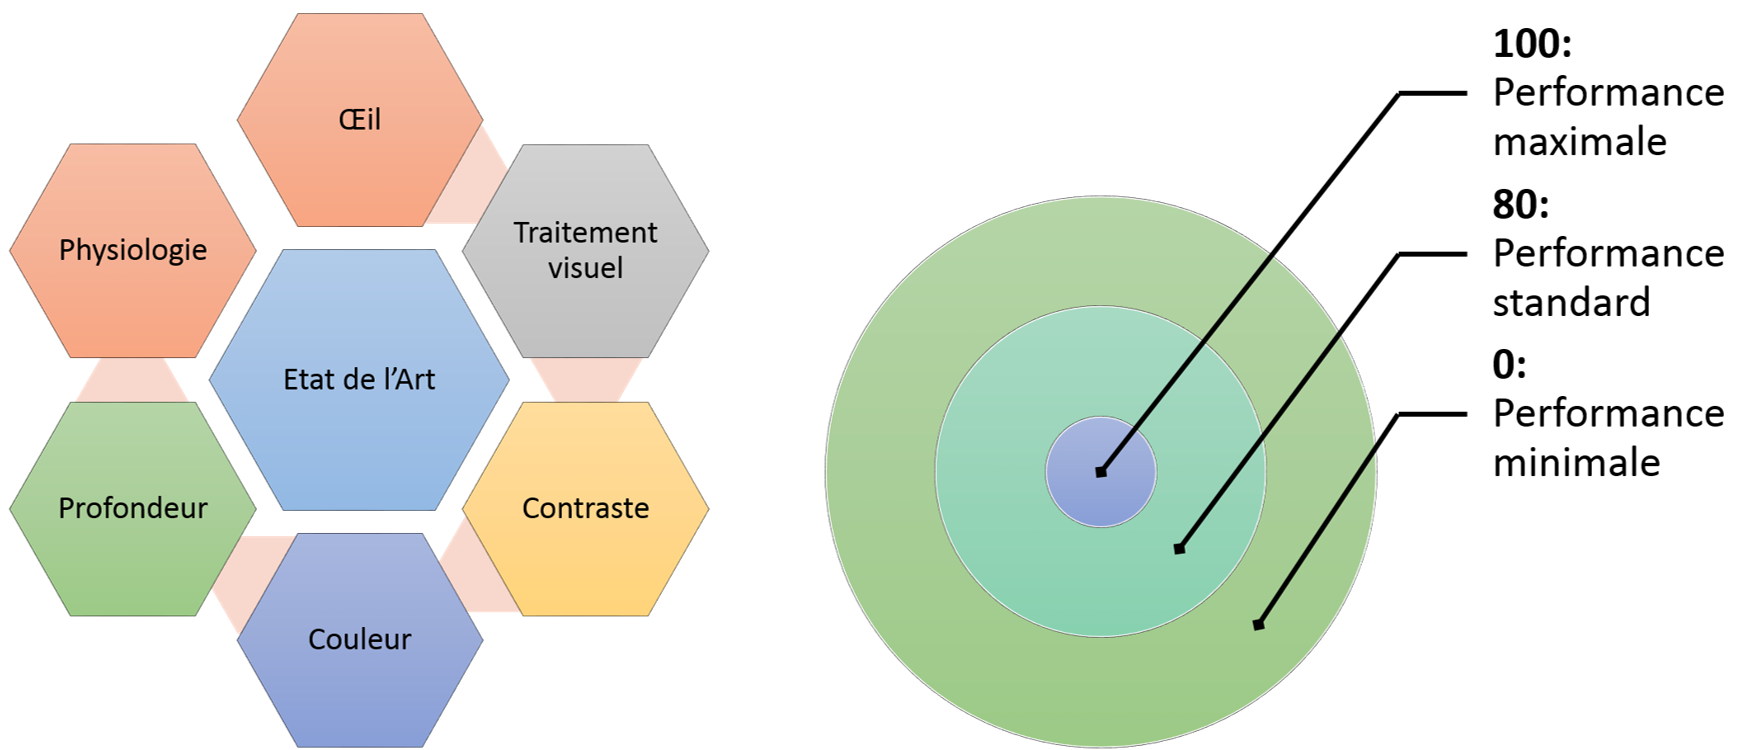
\includegraphics[scale=.50]{Figures/EDLAProcessScoreTarget}
		\caption{Résumé des étapes d'état de l'Art pour la construction du modèle et répartition des objectifs de représentation des notes intermédiaires dans le score de réalisme.}
		\label{fig:edla_process_score_target}
	\end{figure}
	
	\chapter{Proposition de modèle}
	
	\par Pour faciliter la lecture et la compréhension du chapitre, on propose d'expliquer sommairement ici certaines distinctions entre des termes proches qui seront utilisés. Tous ces termes seront explicités en détail par la suite dans les deux prochains chapitres.

	\par L' << acuité monoscopique >>, aussi connue sous le nom d'acuité visuelle est définie par le Vulgaris Médical\footnote{Acuité visuelle. Dans \textit{Vulgaris Médical}. Consulté le 20/09/2017, http://www.vulgaris-medical.com/encyclopedie-medicale/acuite-visuelle (Lien court: https://lc.cx/GfSj)} de la sorte:
	\begin{quote}
		L'acuité visuelle est la capacité de discernement des informations apportées au cerveau par la vue. C'est la performance visuelle, elle mesure le pouvoir de l'œil à distinguer nettement les détails, avec et sans lunettes.
	\end{quote}
	Elle ne doit pas être confondue avec << l'acuité stéréoscopique >> qui est la capacité de l'œil à distinguer une très petite différence de profondeur à une distance donnée.
	
	\par De même, le << champ de vision >> est ce qu'un individu perçoit à un instant $t$ sans possibilité de bouger la tête ou l'œil dans son orbite. Le << champ de regard >> englobe tout ce qu'un individu peut voir en ayant le droit de bouger la tête et les yeux. Par définition, le champ de regard est donc supérieur au champ de vision.
	
	\par Enfin, la gamme dynamique (Dynamic Range en anglais) est, dans le domaine de l'image, le rapport entre le minimum et le maximum de luminance atteignable. Il est définit par rapport à la courbe de gamma obtenue avec un écran cathodique. Le HDR (ou High Dynamic Range) représente un ratio entre le minimum et le maximum de luminance possible supérieur au ratio standard. HDR sous entend en général une technique d'imagerie pour augmenter artificiellement les extrema lumineux pendant la capture d'image.
	
	\section{Propositions préliminaires}	
	\par Avant d'arriver à la modélisation finale du score (voir ci-après) nous sommes passé par un certain nombre de pistes et de modélisations. Nous allons présenter ici les différentes étapes qui ont vu le jour.
	
	\subsection{Première modélisation (Fig. \ref{fig:modèle_1})}
	\par Initialement, la proposition était de faire un score simple qui réunirait les critères de base, accompagné d'un score avancé qui servirait à raffiner l'évaluation du système. La composition du modèle est basée sur les capacités de la vision qui sont l'acuité, l'attention périphérique, la coordination des yeux, la perception de la profondeur, le focus et la perception des couleurs. Si le focus reste un problème insoluble à cause du conflit accommodation-vergence toutes les autres capacités sont néanmoins traitable. Un critère répondant à la coordination des yeux n'est cependant pas encore proposé dans cette première modélisation. Le score simple était alors décliné selon les critères suivants:
	\begin{itemize}
		\item le contraste
		\item l'acuité monoscopique
		\item l'acuité stéréoscopique
		\item la latence
		\item le nombre d'images par seconde
		\item le respect de l'échelle 1:1
		\item la couverture du nombre de couleurs visibles
		\item la taille de l'HDR
	\end{itemize}
	Tandis que le test avancé rajoutait en plus du score simple qui restait à effectuer:
	\begin{itemize}
		\item le champ de vision
		\item le champ de regard
		\item les maximum et minimum de luminance
	\end{itemize}
	Le tout étant rassemblé dans une équation de somme pondérée (Eq. \ref{eq:premiere_modelisation}), avec $\Sigma$ la valeur du score général du système, $\lambda_i$ la pondération du critère $i$, $\sigma_i$ la valeur observée du critère et $F_{100}$ la fonction donnant la note entre 0 et 100 du critère. 
	
	\begin{equation}
		\Sigma = \frac{1}{\sum_{i = 1}^{n} \lambda_i} \sum_{i = 1}^{n} \lambda_i F_{100,i}(\sigma_i)
		\label{eq:premiere_modelisation}
	\end{equation}
	
	\begin{figure}
		\centering
		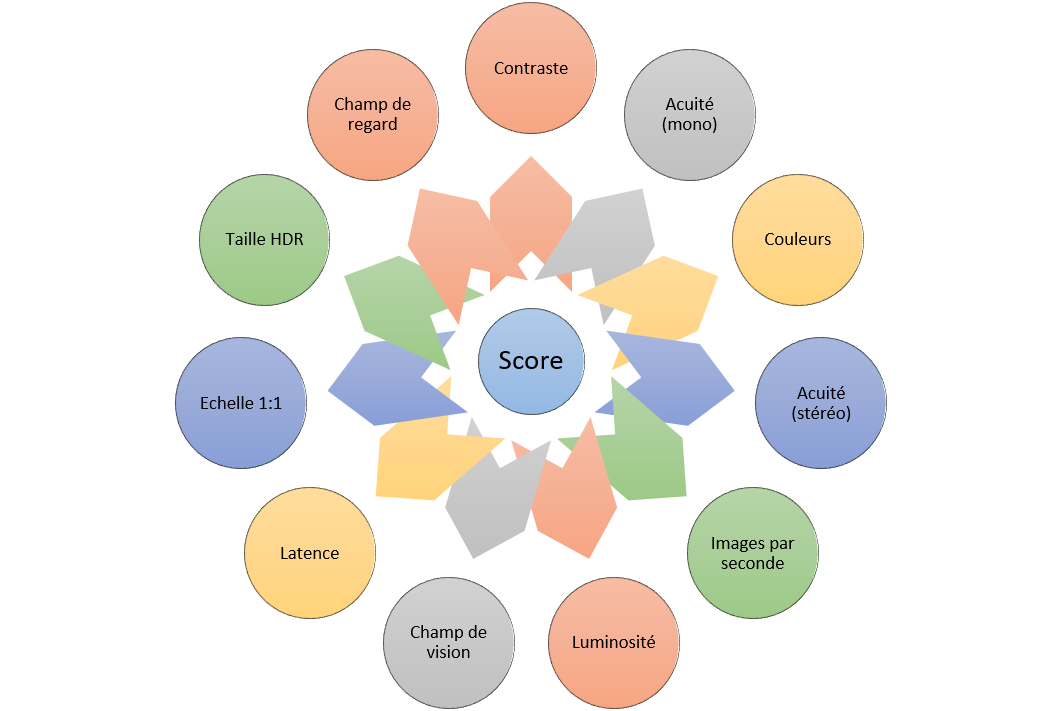
\includegraphics[scale=.8]{Figures/Modele1}
		\caption{Première modélisation du score de réalisme.}
		\label{fig:modèle_1}
	\end{figure}
	
	\subsection{Seconde modélisation (Fig. \ref{fig:modèle_2})}
	\par La seconde étape de la modélisation est assez proche de la première puisqu'on garde une liste quasiment similaire de critères de base : contraste, acuités monoscopique et stéréoscopique, images par seconde, couleur, luminosité et champ de vision. On retire le concept le score simple et de score avancé pour se concentrer sur un mélange des critères des deux scores précédemment envisagés en enlevant cependant les critères de champ de regard, de latence et d'échelle 1:1. Ces trois derniers facteurs sont isolés dans une catégorie appelée << facteurs limitant >> et doivent interdire à la note globale de passer au delà d'un certain seuil en fonction de leur valeur. Ces facteurs sont de type booléens: si le système propose une valeur moins bonne que celle demandé par le facteur limitant, la note globale est automatiquement tronquée.
	
	\par Il était également envisagé de permettre un système de logique combinatoire entre les facteurs limitant. Par exemple, si le score de la latence est inférieur à 50 la note globale est tronquée à 90 alors que si le score de la latence est inférieur à 60 et que le score de champ de regard est inférieur à 40 le score global est tronqué cette fois à 75.
	
	\par C'est à partir de cette modélisation qu'apparaissent les jalons spécifiques de performance: la note de 0 pour le minimum de performance possible ou acceptable, la note de 80 pour la performance standard du système visuel humain et la note de 100 pour sa performance maximale. Un jalon optionnel (en fonction de la littérature) à 60 pour une performance dite << acceptable >> a même été un temps envisagé avant d'être rejeté faute de pertinence et de répétabilité sur tous les critères.
	
	\begin{figure}
		\centering
		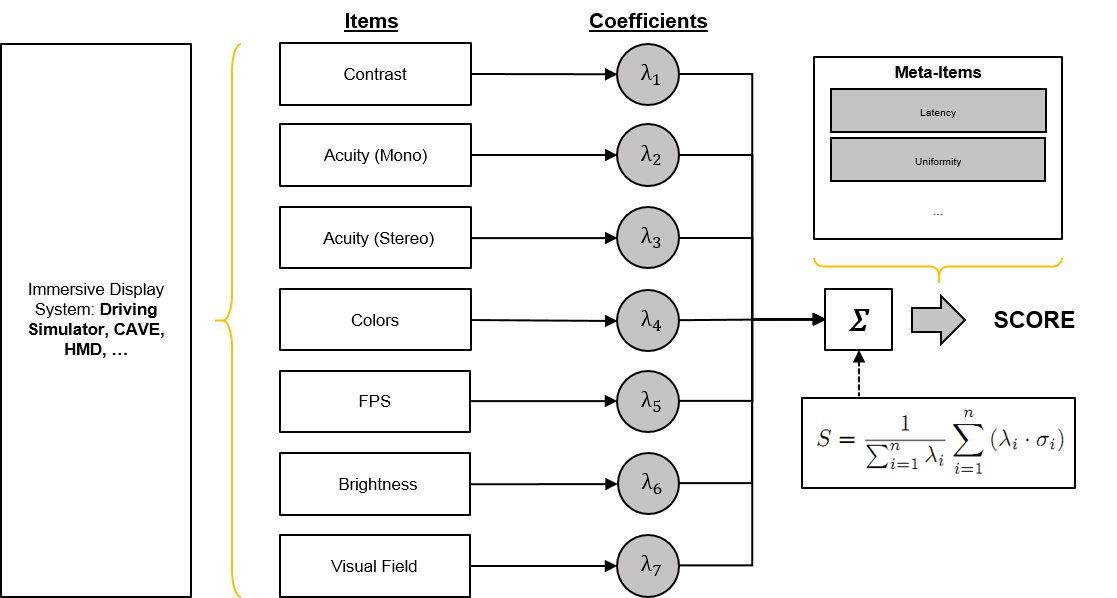
\includegraphics[scale=.8]{Figures/Modele2}
		\caption{Deuxième modélisation du score de réalisme.}
		\label{fig:modèle_2}
	\end{figure}
	
	\subsection{Troisième modélisation (Fig. \ref{fig:modèle_3})}
	\par La troisième modélisation est surement celle qui introduit le plus de changements tant dans la structure que dans la réflexion et le nombre de critères retenus. Le nombre de critère est doublé, passant de 7 à 14. Le concept de facteurs limitant est supprimé. A l'inverse, les critères ne sont plus regroupés en un seul et même ensemble mais sont répartis dans 3 pôles: le pôle << Affichage >>, le pôle << Immersion >> et le pôle << Observateur >>. Pour le pôle observateur on choisi d'extraire des autre pôles et de réunir tous les critères nécessitant des informations sur la personne, typiquement sa position. Par exemple, dans un dispositif de type CAVE, la luminosité reste la même indépendamment où que soit la personne tandis que la taille perçue du pixel dépendra de la distance à l'écran. 
	
	\par Chaque pôle peut ainsi recevoir un score qui lui est propre et le système évalué peut ainsi avoir un score d'affichage honnête mais une mauvaise note en immersion sans que cela dégrade l'évaluation de l'affichage. On met ainsi en évidence trois scores de premier niveau: le score d'affichage, le score d'immersion et le score perceptuel (en rapport avec la catégorie observateur). Les scores d'affichage et d'immersion sont ensuite réunis dans un score technologique, par opposition au score perceptuel pour respecter la dichotomie réalisée entre les critères systémiques pur des critères nécessitant des informations sur l'observateur. Enfin, les scores technologique et perceptuel sont assemblés afin de donner le score global du système immersif évalué.
	
	\par Si la majorité des critères ont une note basée sur des points clef de la littérature, certains points sont plus compliqués à aborder de la sorte étant donné qu'ils ont un fonctionnement plutôt binaire. On les appelle << critères booléens >>. Les critères concernés sont les suivants: tracking, stéréoscopie, vergence et accommodation. Par exemple, le critère de stéréoscopie peut n'être jugé que sur la présence ou l'absence de stéréoscopie dans le système immersif. Pour ce critère en particulier, une piste de recherche sera évoquée plus loin.
	
	\begin{figure}
		\centering
		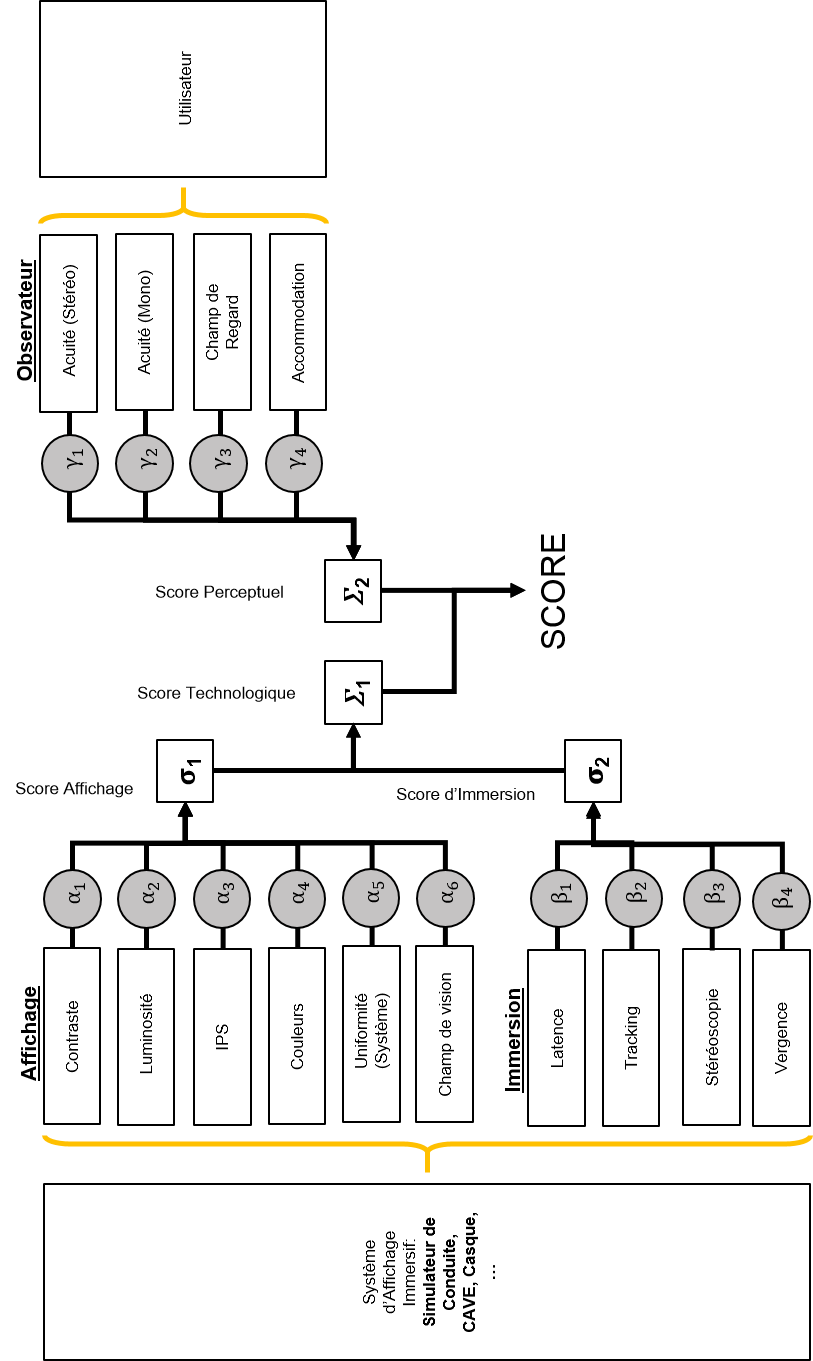
\includegraphics[scale=1]{Figures/Modele3}
		\caption{Troisième modélisation du score de réalisme.}
		\label{fig:modèle_3}
	\end{figure}
	
	\section{Modèle définitif}		
	\par En définitive, après un certain nombre d'itérations, de reconstructions, de nouvelles réflexions et de correction -notamment grâce à l'avis de reviewers des publications qui présentent ce modèle de score- on parvient à une version que l'on estime satisfaisante.
	
	\par On propose un modèle de score divisé en douze critères distribués en deux sections: une partie indices de vision et une partie indices d'immersion. La division des critères est faite telle que la première partie représente les informations qu'un œil recevrait à l'intérieur d'un simulateur tandis que la deuxième catégorie concerne ce que le système immersif offre à l'utilisateur pour participer à l'immersion. L'immersion est évidemment également réalisée via d'autres processus and nous avons seulement couvert les indices liés au hardware. Les critères sont répertoriés comme suit. Une vue d'ensemble du modèle est présentée Fig. \ref{fig:modèle_définitif}.
	
	\begin{itemize}\itemsep12pt
		\item \textbf{Indices de vision:} contraste et luminosité (luminance), images par seconde, nombre de couleurs affichables, champ de vision, acuités monoscopique et stéréoscopique.
		\item \textbf{Indices d'immersion:} latence, champ de regard, stéréoscopie, tracking, uniformité et convergence des caméras (laquelle est directement liée au tracking des yeux).
	\end{itemize}
	
	\par Les critères de luminance et de contraste sont fusionnés. De part la nature du contraste (un ratio de luminances) ces deux critères semblent indissociables. Le critère de vergence est simplement renommé en << convergence des caméras >> car il portait à confusion. Le critère << Accommodation >> qui jugeait de la présence ou non du conflit accommodation-vergence n'était pas pertinent car il n'existe aujourd'hui aucun système permettant de visualiser des images en 3D sans générer ce type de conflit ; il a dont été supprimé.
	
	\par La plus grosse modification reste le passage en deux catégories contre trois dans la précédente modélisation. La catégorie observateur portait à confusion, regroupait des critères qui avaient toute légitimité pour être dans les deux autres catégories. Les critères (moins le critère Accommodation, supprimé) ont donc été redistribués dans leur catégorie légitime. Celles ci sont en plus renommées de manière plus pertinente.
	
	\par Maintenant que nous avons présenté comment le modèle se présentait, il convient de rentrer plus avant dans le détail et de présenter les critères retenus, un par un. A l'image des différentes modélisations du score, on présentera rapidement les étapes de notation quand elles existent.
	
	\begin{figure}
		\centering
		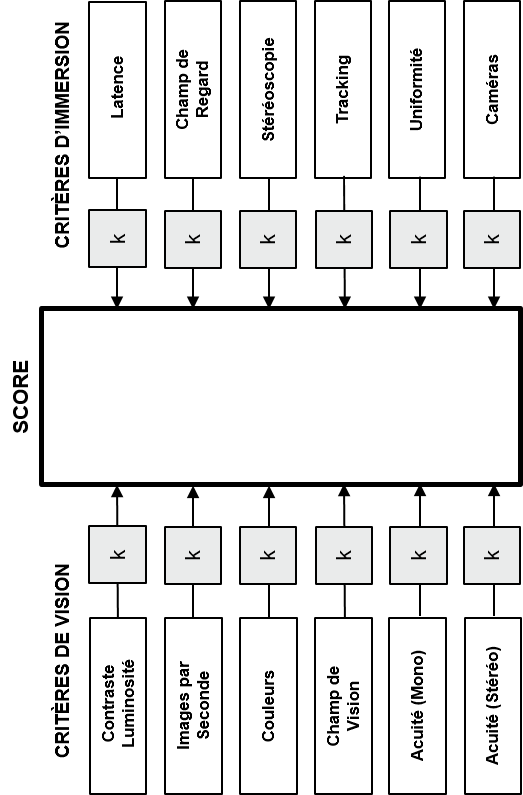
\includegraphics[scale=1.35]{Figures/ModeleDefinitif}
		\caption{Dernière modélisation du score de réalisme.}
		\label{fig:modèle_définitif}
	\end{figure}
		\chapter{Indices de vision}
	\par Nous allons maintenant présenter les différents indices placés dans la catégorie <<~vision~>>, c'est à dire les indices fournis par l'environnement immersif qui participent uniquement à la vision et non pas à l'immersion. Ces indices sont les caractéristiques perçues par un œil fixe et immobile à un instant $t$ dans le simulateur. On présente d'abord les valeurs clefs trouvables dans la littérature puis leur association à ces mêmes valeurs clefs (0, 80 et 100) du modèle, la génération de l'équation permettant d'attribuer la note entre 0 et 100 au critère et, quand c'est possible, le tracé de cette fonction.
	
	\section{Contraste \& luminosité}
	\par Le contraste est théoriquement défini comme la différence en luminosité (ou en couleur) entre les parties claires et les parties sombres d'une image ou d'un objet. Le contraste est un élément très important du système de vision humain, notamment car ce dernier est plus sensible au contraste entre deux niveaux de lumière qu'à un niveau absolu. Comme il peut être fait classiquement en psychophysique, ce stimulus peut être divisé en deux parties: sa magnitude (la valeur brute) et sa résolution (son <<~pas~>> d'évolution).
	
	\par On a pu voir les différentes approches théoriques pour le définir dans la première partie de ce manuscrit. Néanmoins il existe d'autres approches de la gestion du contraste et de la luminance comme par exemple la fonction de sensibilité ou des modèles de performance visuelle. C'est vers ces pistes qu'on s'oriente.
	
	\subsection{Fonction de sensibilité au contraste (CSF)}
	\par Les fonctions de sensibilité au contraste (CSF, pour <<~Contrast Sensibility Functions~>>) sont des courbes traçant le seuil à partir duquel l'œil humain est capable de distinguer une différence entre deux niveaux de gris. La Fig. \ref{fig:fonction_sensibilite_contraste} en est un exemple pour les trois domaines de luminosité: photopique (jour), scotopique (nuit) et mésopique (entre-deux). Tout ce qui se trouve sous la courbe est visible. Elles fonctionnent sur des mesures de seuil en cycles par degré (cpd). Les cpd sont la quantité d'alternance noir-blanc contenue dans un degré visuel.
	
	\begin{figure}[h]
		\centering
		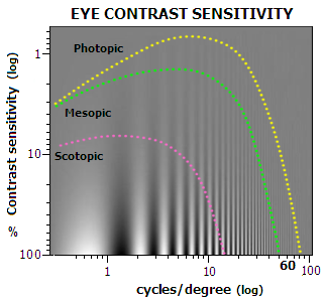
\includegraphics[scale=.9]{Figures/EyeContrastSensitivity}
		\caption{Fonctions de sensibilité au contraste pour les domaines photopiques, scotopiques et mésopiques.}
		\label{fig:fonction_sensibilite_contraste}
	\end{figure}
	
	\par Dans un premier temps, on estime que ces courbes ne sont pas suffisantes car elles ne donnent qu'un seuil en dessous duquel la perception est possible et au dessus duquel elle ne l'est pas. On ne peut en tirer aucune information sur la facilité ou la qualité de vision en dessous du seuil. Que l'on soit très proche ou très éloigné du seuil revient au même: on est dans la catégorie <<~voit~>>. On s'intéresse donc à d'autres approches sur le contraste qui nous permettraient de détailler ce qu'il se passe dans la partie visible du contraste. On s'oriente sur le concept de performance visuelle, que nous allons maintenant présenter.
	
	\subsection{Performance visuelle relative}	
	\par La performance visuelle relative (RVP - Relative Visual Performance en anglais) est définie comme la capacité du système visuel humain à réaliser une tâche donnée, capacité transposée dans une valeur numérique comprise entre 0 et 1. Les paramètres d'entrée du modèle sont en général la luminance et le contraste pour une valeur de sortie unique et sous la forme d'une valeur (comprise entre 0 et 1, donc). De nombreux modèles de performance visuelle ont été développés, notamment dans les années 80, mais deux d'entre eux peuvent être particulièrement mis en avant : le modèle de la CIE (Commission International de l'Eclairage) \citep{international_commission_on_illumination_analytic_1981} et le modèle de Rea \citep{rea_toward_1986}.
	
	\subsubsection{Modèle de la CIE}
	\par Le modèle de la CIE a été construit sur la base d'un grand nombre de résultats expérimentaux issus de nombreux chercheurs différents. Leur but était d'arriver à un outil pour aider à choisir les meilleurs conditions d'illumination pour les ateliers d'usine de manière à ce que les ouvriers travaillent au rendement maximal. En plus de la luminance et du contraste, le modèle nécessite également l'âge et le <<~niveau de demande de la tâche~>> comme paramètres d'entrée.
	
	\subsubsection{Modèles de Rea et Ouellette}
	\par Le modèle de Rea est plus simple mais ses auteurs le déclarent plus précis que celui de la CIE. Leur modèle ne prend en entrée que la luminance de la tâche et la luminance de l'arrière-plan de la tâche. Mark S. Rea présente un première version de son modèle en 1986 \citep{rea_toward_1986} puis une version raffinée en 1991 \citep{rea_relative_1991}. Dans ce dernier modèle, trois paramètres de plus ont été rajoutés: l'âge, la taille de la tâche à réaliser et la luminance d'adaptation (quantité de lumière à laquelle les yeux ont adapté la taille de leur pupille). Ce modèle permet de tracer les graphes visibles en Fig. \ref{fig:courbes_rea}. Ces courbes représentent la performance visuelle en fonction de la luminosité et du contraste pour une taille d'objet vu donnée: la courbe de gauche, plus prononcée, concerne un objet plus petit que celui pour la courbe de droite, moins prononcée.
	
	\begin{figure}[h]
		\centering
		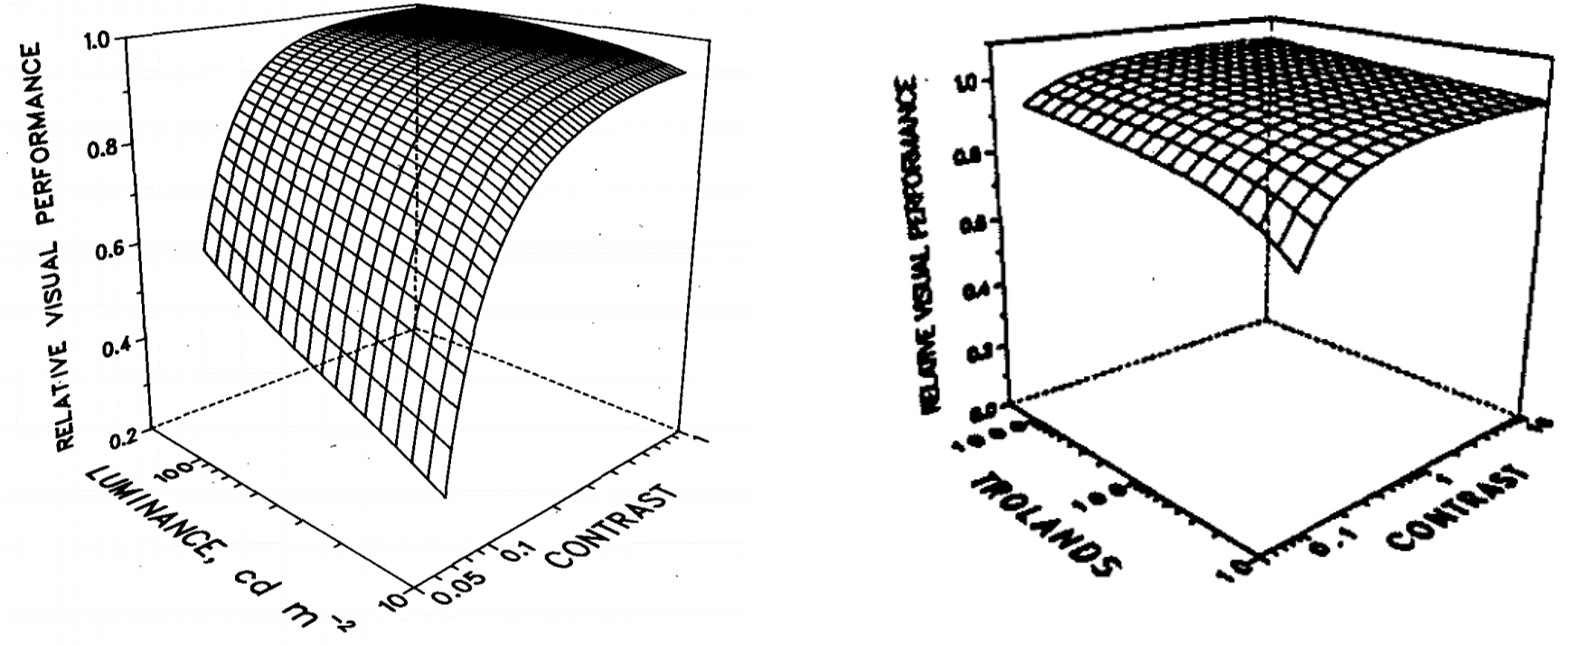
\includegraphics[scale=.5]{Figures/CourbesReaExemple}
		\caption{Exemple de performance visuelle pour deux tailles de cible différentes}{Images tirées de \citep{rea_relative_1991}}
		\label{fig:courbes_rea}
	\end{figure}
	
	\subsubsection{Vers une vérification expérimentale}
	\par Néanmoins, ces deux modèles n'ont pas été pensés pour la Réalité Virtuelle et pourraient ne pas s'inscrire dans pour une utilisation directe dans notre modèle de score de réalisme, en lieu et place du critère de luminance et de contraste. Une expérimentation a été réalisée pour confirmer ou infirmer cette hypothèse, notamment à propos du modèle de Rea (voir partie suivante). L'objectif serait de mettre à l'échelle entre 0 et 100 les résultats entre 0 et 1 du modèle de performance visuelle. Il est à noter que dans son modèle la CIE définit la valeur de 0.8 (80 ramené à notre échelle) comme la performance standard.
	
	\section{Images par seconde}	
	\par Attribuer des valeurs spécifiques, discrètes, aux phénomènes qui composent la vision peut sembler peu naturel tant le processus de vision est continu \citep{bear_neurosciences:_2007}. Néanmoins, c'est un exercice auquel on se risque et il existe un certain nombre d'effets notables qui n'apparaissent qu'à certains nombres d'images par seconde (frame rate).
	
	\subsection{Minimum de fonctionnement}
	\par Premièrement, la perception du mouvement n'est pas basée (comme cela a été suspecté pendant longtemps) sur la persistance rétinienne mais sur deux illusions perceptuelles: l'effet \textit{phi} et le mouvement \textit{bêta} \citep{de_lauretis_flicker_1980}. La persitance rétinienne est un phénomène passif laissant une image rémanente sur la rétine pendant un court instant. L'effet phi est une illusion de mouvement, cette fois active, dans le cerveau et le traitement des images, pour un système en boucle fermée. Le mouvement bêta est lui aussi une illusion d'optique active mais pour les système ouverts. Ces effets sont illustrés en Fig. \ref{fig:beta_phi}). Ils apparaissent à partir de 16 images par seconde. En dessous de cette valeur, aucun mouvement n'est perçu, seulement une suite distincte d'images.
	
	\begin{figure}[h]
		\centering
		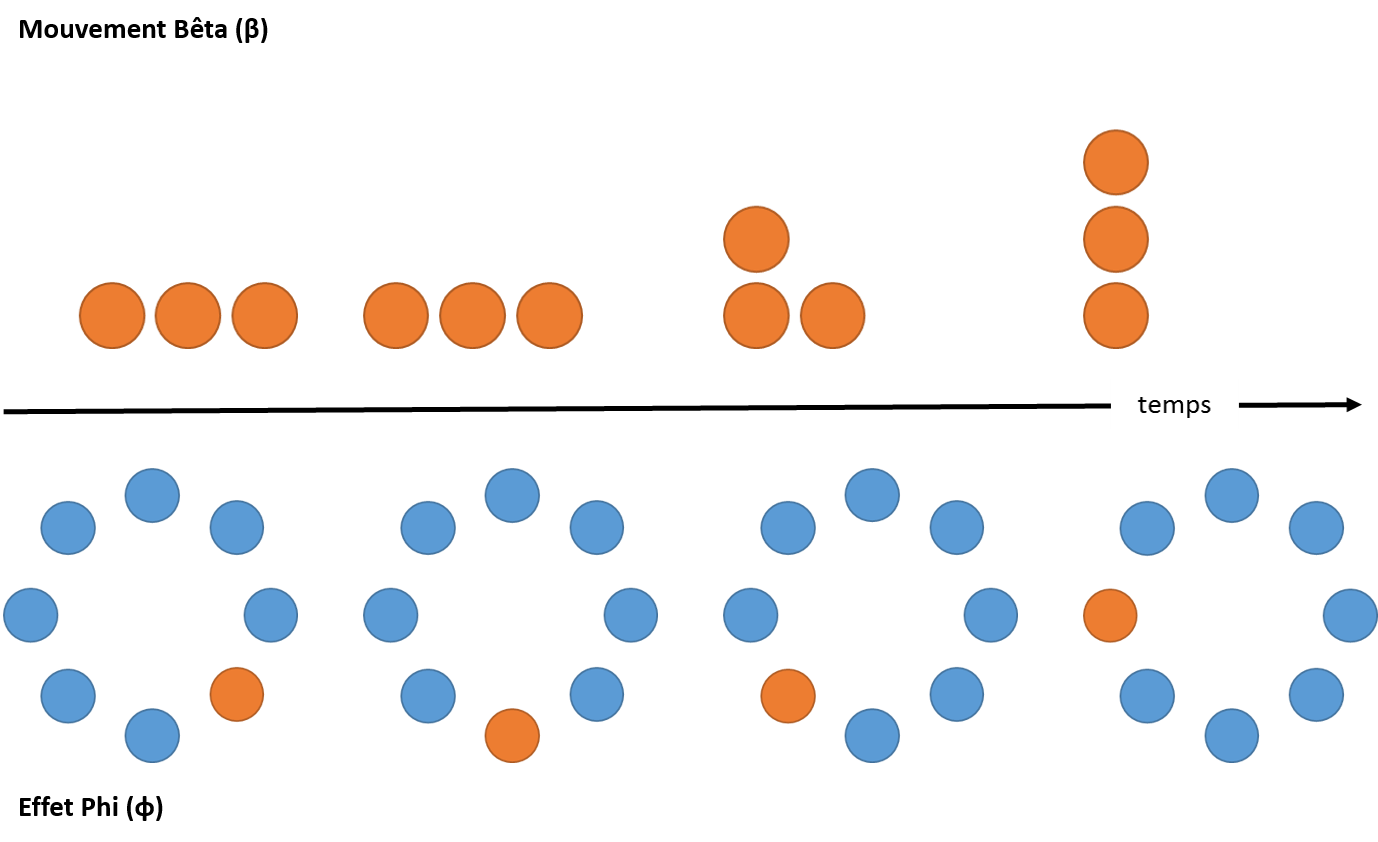
\includegraphics[scale=.65]{Figures/MouvementBetaEffetPhi}
		\caption{Illustration du <<~mouvement beta~>> et de l'<<~effet phi~>>}
		\label{fig:beta_phi}
	\end{figure}
	
	\subsection{Phénomène de scintillement (flickering)}
	\par Deuxièmement, un autre grand phénomène induit par la vision en informatique est le <<~flickering~>>, le clignotement/scintillement de l'écran. Ce phénomène intervient quand le frame rate est trop lent et que l'œil devient capable de percevoir un effet de diminution/changement de luminosité (fading) entre les images. Driscoll \citep{driscoll_eyes_1978}, en s'appuyant sur les travaux de Landis \citep{landis_determinants_1954} et de de Lange \citep{de_lange_dzn_research_1958,de_lange_dzn_research_1958-1}, a travaillé sur la détermination de la fréquence critique de clignotement pour l'œil, c'est à dire la fréquence au delà de laquelle le cerveau ne perçoit plus de clignotement. La fréquence critique de clignotement semble être basée sur un ratio appelé <<~ratio d'ondulation~>> ou <<~ratio ondulatoire~>> (\textit{ripple ratio} en anglais) qui se calcule de la manière suivante (Eq. \ref{eq:ripple_ratio}):
	
	\begin{equation}
	r = \frac{\textrm{Amplitude de l'harmonique fondamentale}}{\textrm{Luminance moyenne}}
	\label{eq:ripple_ratio}
	\end{equation}
	
	\par En utilisant les courbes établies par Driscoll, les courbes de la fonction de transfert de modulation temporelle, quel que soit le ratio ondulatoire, c'est à dire quelle que soit la nature de l'onde lumineuse, la fréquence critique de clignotement, quelle que soit la luminance, est de 70~Hz.
	
	\subsection{Maximum de fonctionnement}	
	\subsubsection{L'hypothèse des deux voies}
	\par D'autres valeurs viennent des voies dorsale et ventrale. Pour rappel, la théorie des deux voies est le postulat principal permettant d'expliquer la manière dont le cerveau traite les informations visuelles arrivant des nerfs optiques. Une fois dans le cerveau, l'information est divisée en deux boucles de traitement \citep{ingle_two_1982,dhondt_emotion_2011}. La première, la voie dorsale ou pariétale, est la boucle <<~où~>> et s'occupe d'extraire la direction et le mouvement du flux d'image qui arrive. L'autre voie, la voie ventrale ou temporale, dite boucle du <<~quoi~>>, s'occupe d'extraire la forme, la couleur et la texture. Les deux voies fonctionnent supposément à des fréquences autour de, respectivement, 200~Hz et 25~Hz, ce qui est corrélé par le fait que l'une est rapide et l'autre lente \citep{dhondt_emotion_2011}, par le nombre de cortex différents par lesquels ces voies passent \citep{dhondt_emotion_2011} et par les latences propres de chaque cortex \citep{bullier_integrated_2001} ; cependant, aucunes valeurs précises n'ont été scientifiquement établies.
	
	\subsubsection{Les pilotes de l'US Air Force}	
	Parallèlement, l'US Air Force aurait conduit des expériences sur ses pilotes de chasse pendant lesquelles ceux-ci étaient capables de reconnaitre un modèle d'avion sur des images flashées à 1/220ème de seconde\footnote{Human Eye Frames Per Second. Dans \textit{AMO.net America's Multimedia Online}. Vu sur \url{http://amo.net/nt/02-21-01fps.html}}. Même si cela ne constitue pas une preuve scientifique en tant que telle, cela vient renforcer l'hypothèse des deux voies sur la fréquence maximale associable au traitement visuel. A la différence du minimum de fonctionnement où des phénomènes sont clairement établis avec des fréquences de fonctionnement claires, on ne peut ici fonctionner que sur des approximations.
		
	\subsection{Fonction de notation du critère}
	\par Ainsi, en utilisant les trois valeurs clefs précédemment présentées: le nombre minimal de fréquence d'image pour percevoir le mouvement (16~Hz), la fréquence critique de clignotement (70~Hz) et la fréquence supposée de la voie dorsale (200~Hz), on peut assembler un modèle mathématique et en tirer une courbe. Dans le cas de ce critère, avec $f$ le nombre d'images par seconde du système de visualisation, on présente l'équation suivante (Eq. \ref{eq:fps_score}), dont le tracé est donné en Fig. \ref{fig:score_fps}:
	\begin{equation}
		F_{FPS}(f) = \begin{cases}
		0 & f < 16\\
		126.5 - \frac{367.1}{\sqrt{f - 7.6}} & sinon\\
		100 & f > 200
		\end{cases}
		\label{eq:fps_score}
	\end{equation}

	\begin{figure}[h]
		\centering
		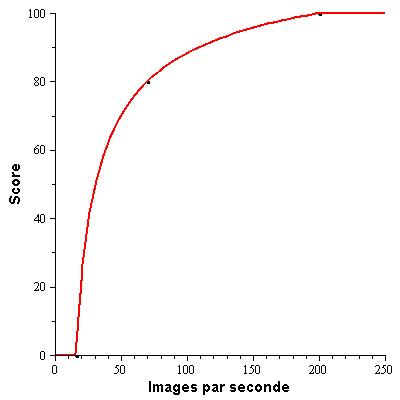
\includegraphics[scale=.75]{Figures/FPS}
		\caption{Tracé de la fonction de notation du critère <<~images par seconde~>>}
		\label{fig:score_fps}
	\end{figure}

	\par Finalement, il doit être noté que toutes ces valeurs clefs sont définies pour un œil unique et donc qu'elles doivent être multipliées par deux dans le cas d'une application à la VR utilisant la stéréoscopie active (c'est à dire avec une image sur deux présentée à chaque œil) pour une imagerie 3D. %De plus, ces fréquences sont les nombres d'images par seconde effectifs, c'est à dire ceux qui sont réellement affichés par l'écran et non pas les nombres d'images par seconde du hardware (en sortie de carte graphique par exemple) qui sont en général plus élevés à cause du principe de Shannon (plusieurs occurrences d'un signal sont nécessaires pour son échantillonnage).
	
	\section{Couleurs}
	\subsection{Dénombrement des couleurs visibles}	
	\par La première approche serait d' essayer d'estimer le nombre de couleurs réellement visibles (discernables) par un œil humain. Cette entreprise a été tentée un certain nombre de fois \citep{kuehni_how_2015, linhares_number_2008, perales_calculation_2008, pointer_gamut_1980, pointer_number_1998, wen_display_2006} sans jamais faire preuve de beaucoup de succès: les estimations varient entre 100.000 et 10 millions de couleurs visibles.
	
	\par Les estimations se font mathématiquement: soit en utilisant les équations de différentiation des couleurs, soit en recalculant des observateurs réels pour les comparer à l'observateur idéal établi par la CIE (voir la première partie et le chapitre sur la couleur).
	
	\subsection{Les espaces colorimétriques}
	\par A défaut d'avoir une estimation validée du nombre de couleurs perceptibles et de pouvoir proposer une méthode pour calculer facilement ce même nombre dans un simulateur pour ensuite les comparer, on se tourne vers les espaces colorimétriques.
	
	\par En 1931, la Commission Internationale de l'Eclairage (CIE) a établi la définition de l'espace colorimétrique RGB. Cet espace de couleur représente l'ensemble des couleurs (non dénombrées) qui peuvent être vues par un observateur normal possédant les trois types de cônes. Cependant, il n'existe encore aucune technique pour afficher 100\% des couleurs théoriquement incluses dans l'espace RGB. Chaque système utilise une fraction de cet espace de couleur qu'on appelle <<~gamut~>> et qui dépend de trois (ou plus suivant les espaces) couleurs primaires choisies spécifiquement par la norme (Fig. \ref{fig:multi_gamut}). Dans la table suivante (Table. \ref{tab:gamut}), on présente un certain nombre de normes avec la proportion d'espace colorimétrique couverte par leur gamut. Il est à noter que dans le cas de la norme ProPhoto RGB, 13\% des couleurs atteignables sont en fait des couleurs imaginaires à cause de couleurs primaires qui sont prises hors de l'espace RGB de 1931. Empiriquement, l'acceptation commence à partir d'Adobe RGB.

	\begin{table}[h]	
		\centering
		\caption{Gamuts Coverage of 1931 Color Space}
		\label{tab:gamut}
		\small
		\begin{tabular}{ll}
			BR.709 (HDTV) & 35.9\%\\
			Adobe RGB & 52.1\%\\
			Digital Cinema & 53.6\%\\
			BT.2020 (UHD) & 75.8\%\\
			Wide-Gamut RGB & 77.6\%\\
			ProPhoto RGB & 90.0\%\\
		\end{tabular}
	\end{table}
	
	\begin{figure}[h]
		\centering
		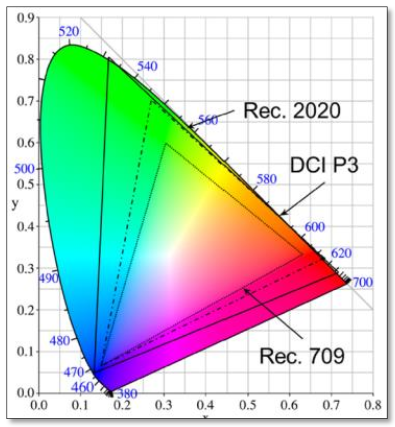
\includegraphics[scale=.9]{Figures/GamutBT2020}
		\caption{Tracé de différents gamuts sur l'espace colorimétrique CIE RGB 1931.}
		\label{fig:multi_gamut}
	\end{figure}
	
	\subsection{Indice de rendu des couleurs (IRC)}
	\par La piste de l'indice de rendu des couleurs (IRC) est une piste élégante, qui, à l'instar du critère de contraste et de luminosité propose une méthode donnant directement une valeur entre 0 et 1 et donc transposable au score de réalisme.
	
	\par Néanmoins, l'IRC est une valeur qui compare le spectre lumineux d'une lampe (dans notre cas, cela pourrait être un projecteur dans un simulateur) avec le spectre d'une lampe de référence, sensé être complet. Il y a donc principalement deux problèmes qui nous empêchent d'implémenter cette solution dans notre modèle: l'indice est dévolu aux lampes et non aux écrans, ce qui restreindrait le champ d'action de notre score de réalisme ; et surtout, la comparaison est faite par rapport à une lampe idéale et non par rapport au système visuel humain. On laisse donc de côté cette piste pour revenir à une modélisation plus simple mais plus proche de l'objectif fixé de proximité avec le système visuel humain. 
	
	\subsection{Fonction de notation du critère}
	\par Notre proposition de notation pour le critère de couleur est donc réduite à une fonction continue entre le score et le pourcentage de couverture de l'espace RGB 1931 auquel le système peut prétendre (Fig. \ref{fig:score_color}). Ce pourcentage vient directement de-s espace-s colorimétrique-s impliqué-s dans la chaine de rendu et d'affichage. On attribue la note maximale à la couverture totale de l'espace théorique des couleurs perçues par l'oeil humain et la note minimale à la couverture nulle. La note équivalente à la performance standard est attribuée au seuil d'acceptation remarqué, soit 52.1\%. La fonction de score pour ce critère est donc, avec $c$ le pourcentage de couverture de RGB 1931 par le gamut:
	 \begin{equation}
		F_{color}(c) = \begin{cases}		
		0.00002 \times c^3 -0.01 \times c^2 + 2.2 \times c &\\
		100 & c > 100
		\end{cases}
		\label{eq:color}
	\end{equation}
	
	\par Il pourrait être intéressant de réaliser une expérimentation sur les besoins en couleurs (à différentier de l'appréciation du nombre de couleurs) en comparant par exemple des populations novices avec des populations expertes. Néanmoins faute de temps et de moyens (aujourd'hui encore aucun appareil commercial n'est capable d'afficher l'intégralité de l'espace RGB 1931) ce ne sera pas réalisable le temps de la thèse.
	
	\begin{figure}[h]
		\centering
		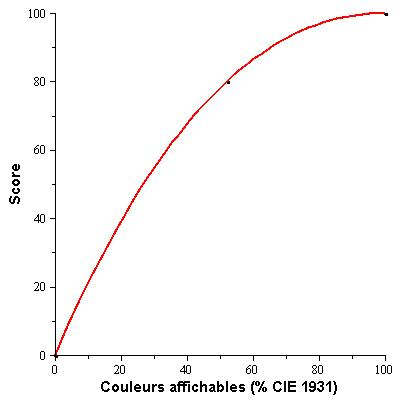
\includegraphics[scale=.75]{Figures/Color_2}
		\caption{Tracé de la fonction de notation du critère <<~couleurs~>>}
		\label{fig:score_color}
	\end{figure}
	
	\section{Champ de vision}
	\par Le champ de vision (FOV - Field of View en anglais) est défini comme la portion d'espace qu'une personne peut voir à un instant t, sans bouger la tête. Il ne doit pas être confondu avec le champ de regard (FOR - Field of Regard en anglais) qui est la portion d'espace totale que l'on peut voir au cours du temps lorsque les mouvements de la tête et des yeux sont pris en compte.

	\par Le champ de vision se décompose en deux orientations: l'axe vertical et l'axe horizontal. On propose deux ensembles de valeurs, un par axe, pour la notation. Les deux axes seront ensuite pondérés l'un par rapport à l'autre. On fait l'hypothèse dans un premier temps que cette pondération se fait par rapport à leur taille respective. La valeur du champ de vision que l'on mesure pour introduire dans le score doit être prise pour la position standard du sujet dans l'environnement immersif (que ce soit la position du corps ou l'orientation de la tête).
	
	\subsection{Axe horizontal}
	\par Certaines des valeurs les plus communes admises pour le champ de vision horizontal sont recensées chez \citep{devisme_optimisation_2004}. Sur l'angle d'azimut (horizontal), avec les deux yeux, un être humain normal peux voir sur 170 à 190 degrés. A l'intérieur de cet angle d'azimut, seuls 120 degrés (centrés) permettent de voir binoculairement. La vision binoculaire est possible grâce à la superposition des portions d'espace vues par chaque oeil simultanément. L'acuité maximale est atteinte dans la zone fovéale soit entre 3 et 5 degrés de portion d'espace, au centre de la vision. La lecture n'est possible que dans un angle de 20 degrés tandis que la reconnaissance des formes est possible jusqu'à 40 degrés et la reconnaissance des couleurs jusqu'à 60 degrés. Ces différentes valeurs sont résumées dans la Fig. \ref{fig:champ_vision_horizontal}. L'équation propre à l'axe horizontal est, avec $h$ la valeur en degrés du champ de vision horizontal (H-FOV) calculé dans le système immersif (Eq. \ref{eq:score_h_fov}):
	\begin{equation}
	F_h(h) = \begin{cases}
		0 & h < 20\\
		19.6 \sqrt{h} -0.5 \cdot h -78.3 & sinon\\
		100 & h > 180
	\end{cases}
	\label{eq:score_h_fov}
	\end{equation}
	
	\begin{figure}[h]
		\centering
		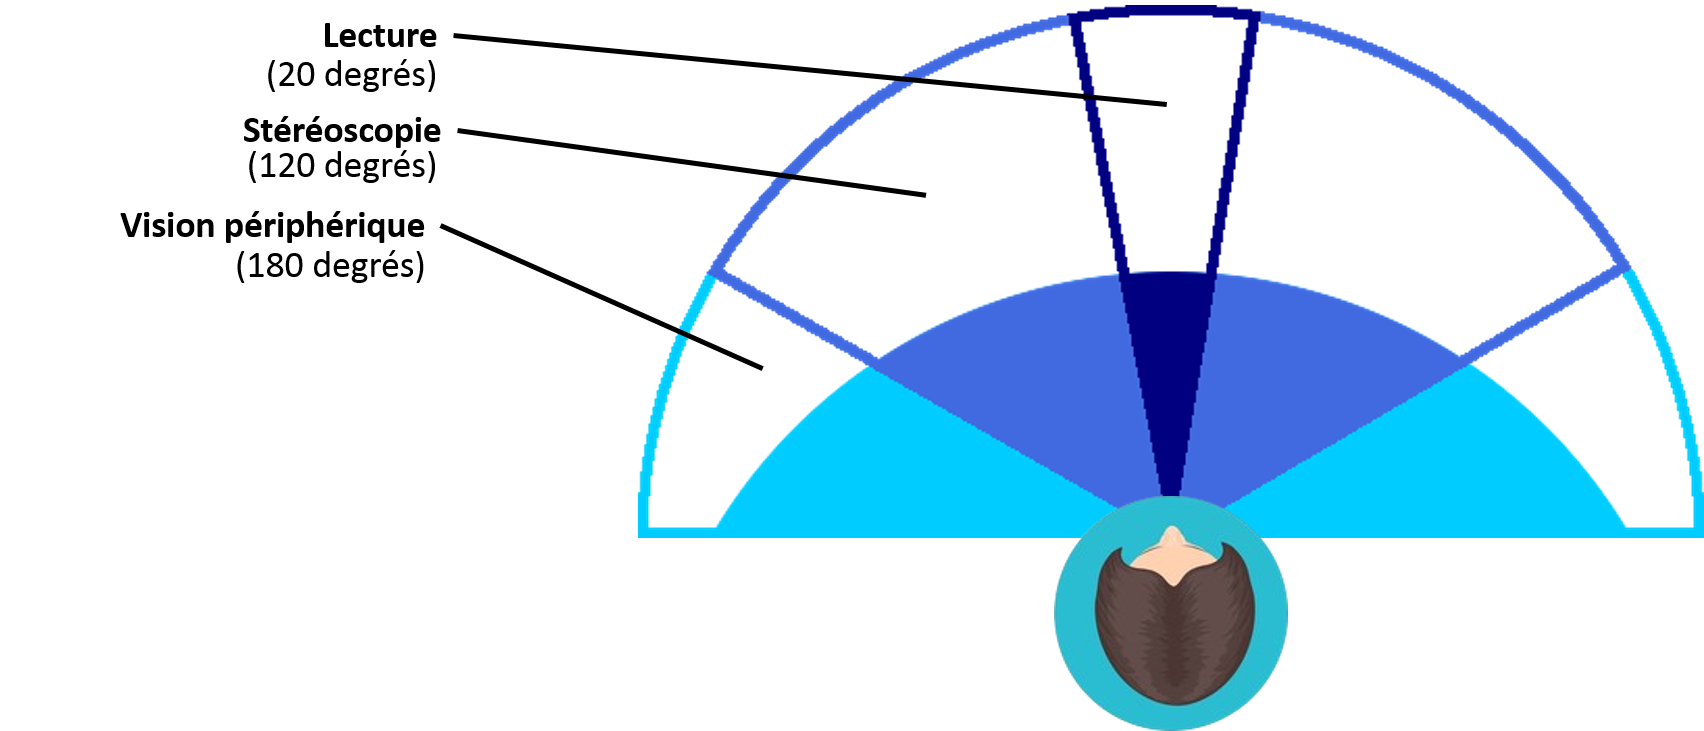
\includegraphics[scale=.5]{Figures/ChampVisionHorizontal}
		\caption{Répartition des zones visuelles sur l'axe horizontal du champ de vision.}
		\label{fig:champ_vision_horizontal}
	\end{figure}

	\subsection{Axe vertical}
	\par On retient trois valeurs caractéristiques parmi les nombreuses qu'on peut trouver dans la littérature pour le champ de vision vertical. La première correspond à la totalité de la vision latérale sur l'axe vertical: 130 degrés. On retient aussi les angles d'impression induite (85 degrés) et de vigilance (20 degrés) \citep{langlois_adas_2013} (Fig. \ref{fig:champ_vision_vertical}). L'équation propre à l'axe vertical est, avec $v$ la valeur en degrés du champ de vision vertical (V-FOV) (Eq. \ref{eq:score_v_fov}): 
	\begin{equation}
	F_v(v) = \begin{cases}
	0 & v < 20\\
	32.0 \sqrt{v} -1.1 \cdot v -121.1 & sinon\\
	100 & v > 130
	\end{cases}
	\label{eq:score_v_fov}
	\end{equation}
	
	\begin{figure}[h]
		\centering
		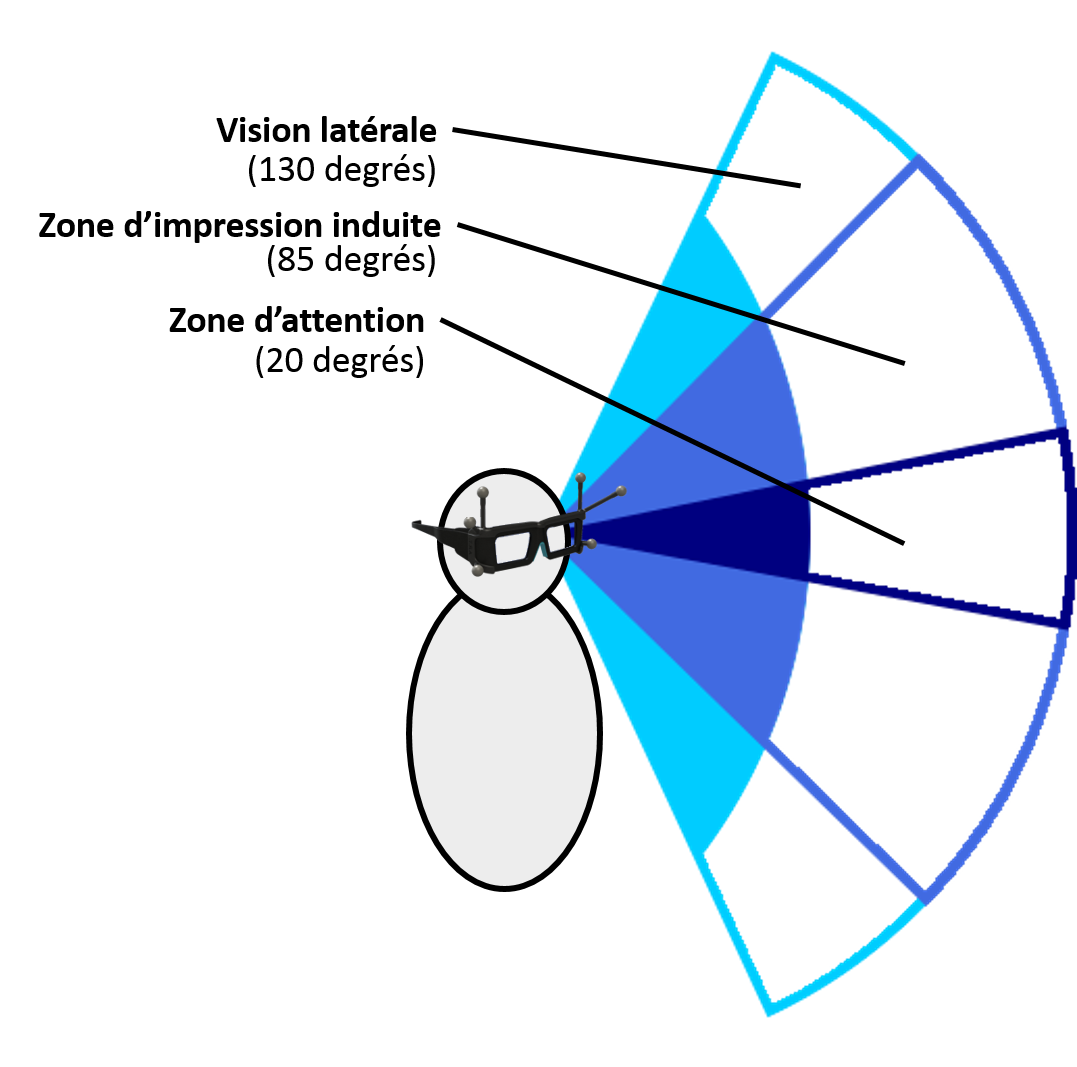
\includegraphics[scale=.6]{Figures/ChampVisionVertical}
		\caption{Répartition des zones visuelles sur l'axe vertical du champ de vision.}
		\label{fig:champ_vision_vertical}
	\end{figure}
	
	\subsection{Pondération}
	\par On pose notre propre hypothèse d'égale importance des axes verticaux et horizontaux dans le champ de vision. Cette hypothèse est une sorte de <<~cas général~>>. On verra par la suite que l'on sera amené à la modifier. On pondère donc les deux sous-critères en fonction de leur taille maximale respective (180 degrés pour l'axe horizontal et 130 pour l'axe vertical) (Eq. \ref{eq:coeff_fov}):
	\begin{equation}
		\begin{cases}	
			k_h = \frac{180}{180 + 130} = 0.58\\
			k_v = 1 - k_h = 0.42
		\end{cases}
		\label{eq:coeff_fov}
	\end{equation}
	
	\subsection{Fonction de notation du critère}
	\par Au final, la fonction de notation du critère de champ de vision est l'agrégation des précédentes équations via une pondération et s'apparente comme suit (Eq. \ref{eq:score_fov}):
	\begin{equation}
	F_{FOV}(h,v) = k_h \cdot F_h(h) + k_v \cdot F_v(v)
	\label{eq:score_fov}
	\end{equation}

	\begin{figure}[h]
		\centering
		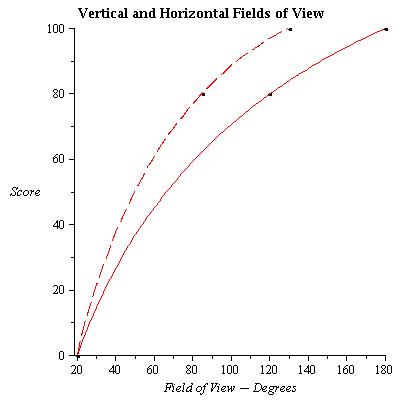
\includegraphics[scale=.75]{Figures/FOV}
		\caption{Tracé de la sous-fonction horizontale de notation du critère <<~champ de vision~>> (ligne continue) et de la sous-fonction verticale (pointillés).}
		\label{fig:score_fov}
	\end{figure}
	
	\section{Acuité monoscopique}
	
	\subsection{Première approche}	
	\par Notre première approche était de se raccrocher à un tableau établi par la <<~classification internationale des maladies~>> (CIM), publié par l'Organisation Mondiale de la Santé (OMS). L'objectif est de permettre l'analyse systématique des maladies et autres affections du corps. On s'intéresse ici à la partie relative aux trouble de la vision et plus particulièrement à l'acuité. On utilise la version cliniquement modifiée de la 9ème révision de cette classification, ICD-9-CM, sortie en 1975. La 10ème révision, ICD-10 ne faisant pas encore l'unanimité et ne rajoutant que d'autres entrées sans modifier celle ci.
	
	\par La Fig. \ref{fig:icd_9_cdm} montre les différentes acuités possibles pour l'œil humain (encadré en bleu), associées avec le type de vision et surtout un score équivalent (encadré en bleu). Ce score est néanmoins peu adapté à notre utilisation, d'abord parce qu'il dépasse la note de 100 mais surtout parce qu'il englobe des acuités bien trop faibles pour être transposées en taille de pixel dans un simulateur. De plus il correspond à des défauts de vision plus qu'à des capacités de vision. On s'oriente alors vers une autre approche.
	
	\begin{figure}[h]
		\centering
		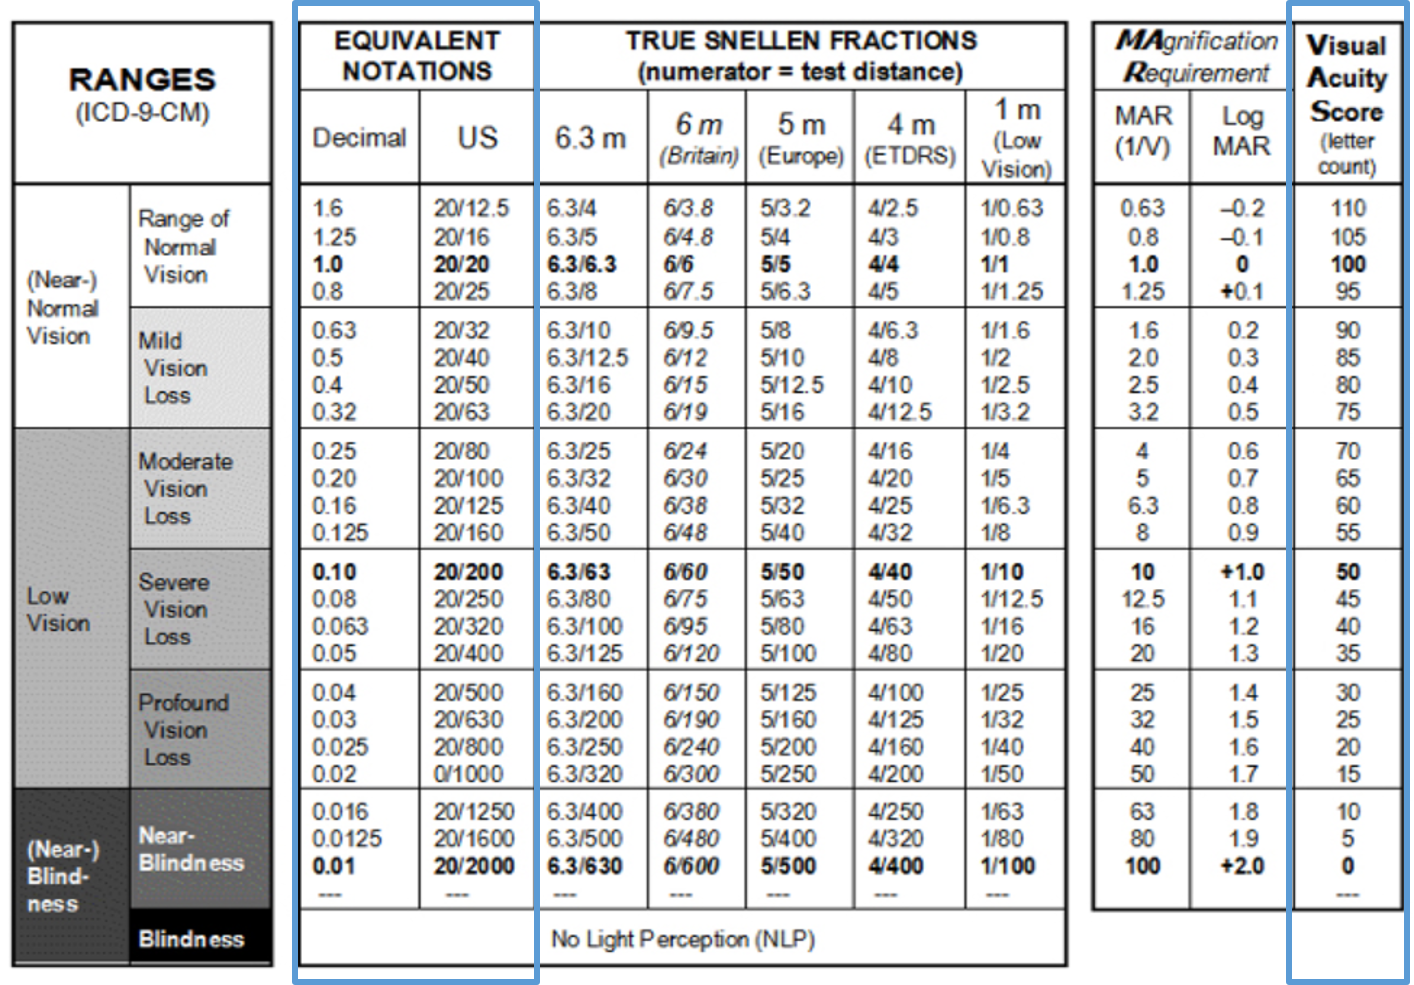
\includegraphics[scale=.6]{Figures/AcuityICD9CM}
		\caption{Classification ICD-9-CM}{On cherche à établir un lien entre les colonnes encadrées: l'acuité, et le score.}
		\label{fig:icd_9_cdm}
	\end{figure}
	
	\subsection{Deuxième approche}
	\par L'acuité monoscopique est la précision de l'œil humain, sa résolution ; c'est à dire à quel point la plus petite chose qui peut être vue peut être petite ou bien quelle est le plus petit écart perceptible entre deux motifs. Ce concept peut être directement lié à la taille du pixel sur un écran: plus le pixel est petit plus l'image est précise. Néanmoins, à partir d'une certaine taille, le pixel devient plus petit que la résolution de l'œil et devient alors non-discernable individuellement, et donc, pas forcément très utile.
	
	\par Habituellement, on estime que le système visuel humain a une acuité monoscopique comprise entre 30 secondes d'arc et 2 minutes d'arc, avec une moyenne à 1 minute d'arc \citep{fuchs_traite_2003}. Ces valeurs peuvent être, dans des conditions photopiques d'éclairage, raffinées en fonction de la tâche \citep{gross_human_2008} (voir Tab. \ref{tab:acuity}).

	\begin{table}[h]
		\centering
		\caption{Acuité de l'œil, \citep{gross_human_2008}}
		\label{tab:acuity}
		\small
		\begin{tabular}{ll}
			\multicolumn{1}{c}{\bfseries Task} & \multicolumn{1}{c}{\bfseries Acuity}\\
			Reconnaissance de forme & 5'\\
			Résolution d'une grille & 2'\\
			Résolution deux points (couleurs identiques) & 1'\\
			Résolution deux points (couleurs inversées) & 30"\\
			Acuité de Vernier (fines lignes droites parallèles) & 10"\\
			Acuité stéréoscopique & 5"\\
		\end{tabular}
	\end{table}
	
	\par La résolution de Vernier n'est atteignable que dans certaines conditions spécifiques et l'acuité stéréoscopique est un sujet à part, traité avec une autre approche, décrite dans la section suivante. De plus, Deering a montré que la plus petite résolution possible sur un écran est de 28 secondes d'arc \citep{deering_limits_1998}. C'est pourquoi on ne retient que les valeurs entre 5 minutes d'arc et 30 secondes d'arc.
	
	\subsection{Fonction de notation du critère}
	\par L'équation qui est proposée depuis ces valeurs, avec $\alpha$ l'angle sous lequel le pixel est vu, en minute d'arc (Eq. \ref{eq:mono_acuity_score}, tracé en Fig. \ref{fig:score_mono_acuity}) est la suivante:
	
	\begin{equation}
		F_{acuite\_mono}(\alpha) = \begin{cases}
		0 & \alpha > 3.5\\
		128.9 - 68.8 \sqrt{\alpha} - \frac{0.1}{\alpha} & sinon\\
		100 & \alpha < \frac{1}{6}
		\end{cases}
		\label{eq:mono_acuity_score}
	\end{equation}

	\begin{figure}[h]
		\centering
		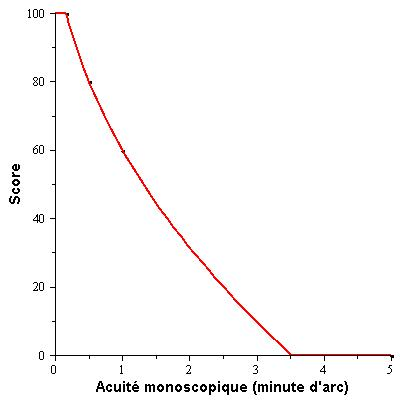
\includegraphics[scale=.75]{Figures/AcuityMono}
		\caption{Tracé de la fonction de notation du critère <<~acuité monoscopique~>>}
		\label{fig:score_mono_acuity}
	\end{figure}
	
	\section{Acuité stéréoscopique}
	\subsection{Première modélisation}	
	\subsubsection{Modèle usuel}	
	\par L'acuité stéréoscopique est la capacité du système visuel humain à percevoir une différence de profondeur entre deux plans, à une distance donnée. C'est une caractéristique qui est largement connue et décrite dans la littérature. Sa description mathématique vient d'une analyse géométrique simple \citep{fuchs_traite_2003,gross_human_2008}. Le modèle globalement accepté est le suivant (Eq. \ref{eq:stereo_model}):

	\begin{equation}	
		\Delta r = 0.001 \times r^2
		\label{eq:stereo_model}
	\end{equation}
	 
	\par Avec $\Delta r$ la différence minimale théorique de différence en profondeur (en millimètres) et $r$ la distance d'observation en mètres. Le facteur 0.001 est le rapport entre le seuil physiologique de la vision stéréoscopique ($\Delta \nu_{min}$) et la distance inter-pupillaire (DIO).
	
	\subsubsection{Limites et solution d'amélioration}
	\par Cependant, ces deux derniers paramètres peuvent varier de manière significative: la distance inter-pupillaire varie de 52 à 78~mm sur toute la population \citep{dodgson_variation_2004} (Fig. \ref{fig:variation_dio_population}) tandis que le seuil physiologique de vision dépend de la luminance, notamment quand celle ci est à un niveau très bas \citep{gross_human_2008}. On peut néanmoins conserver la valeur de 0.001 comme constante dans le modèle car la variation suivant les deux paramètres est assez faible (Fig. \ref{fig:variation_constante_dio}).
	
	\begin{figure}[h]
		\centering
		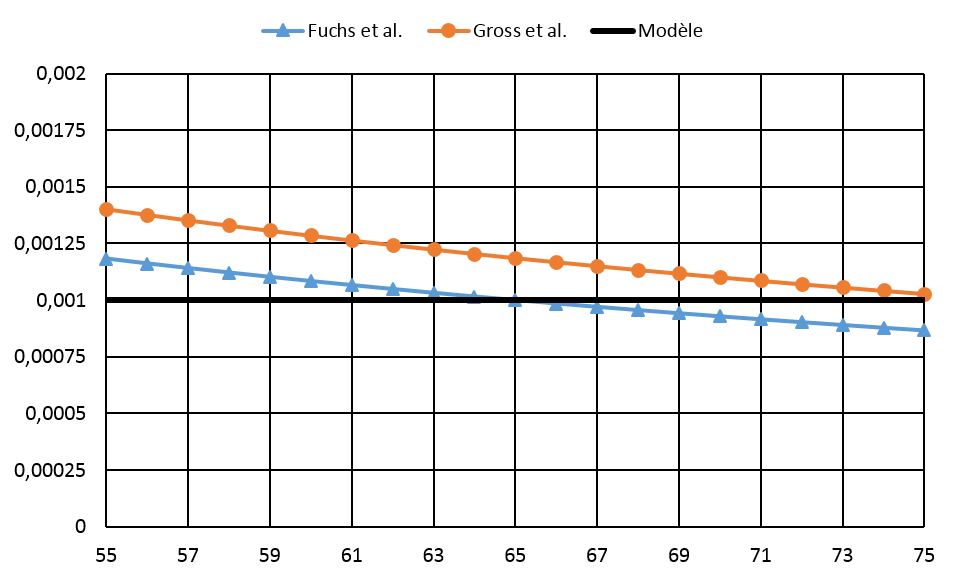
\includegraphics[scale=.9]{Figures/FractionVariation}
		\caption{Variation de la constante du modèle d'acuité stéréoscopique en fonction de la distance interoculaire.}
		\label{fig:variation_constante_dio}
	\end{figure}
	
	\begin{figure}[h]
		\centering
		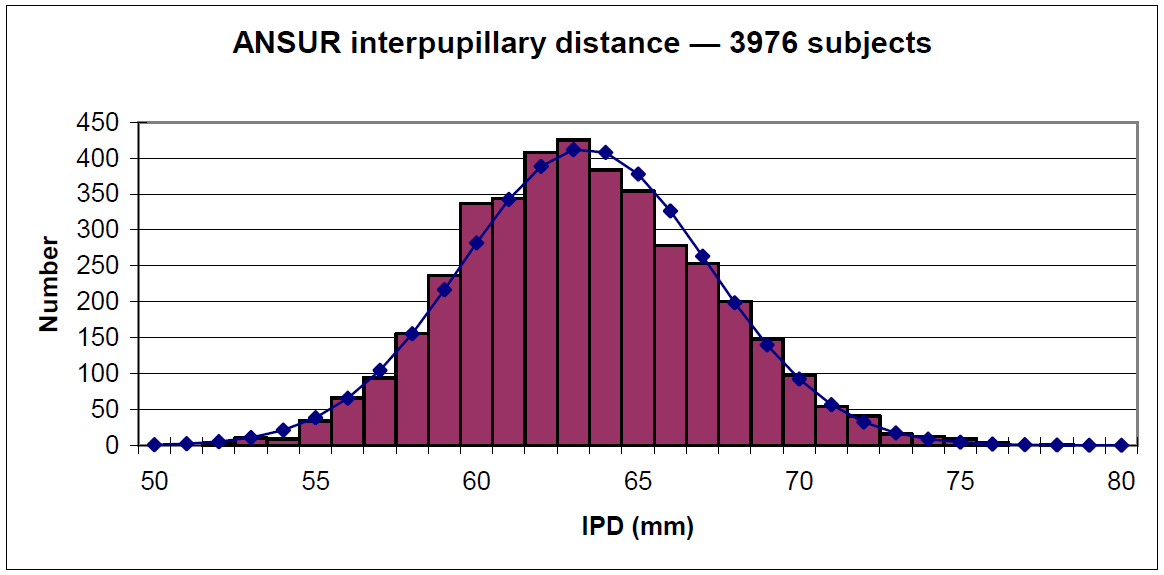
\includegraphics[scale=.5]{Figures/ANSURIPD}
		\caption{Variation de la distance interoculaire sur la population. Image tirée de \citep{dodgson_variation_2004}}
		\label{fig:variation_dio_population}
	\end{figure}
	
	\par De plus, un processus standardisé pour mesurer la valeur de $\Delta r$ d'un système serait difficile à mettre en place car il faudrait faire passer un test à un certain nombre de sujets puis en extraire le seuil moyen expérimental, ce qui sort du cahier des charges du score de réalisme. En travaillant la relation qui décrit ce même modèle d'acuité stéréoscopique (Eq. \ref{eq:limiting_angle}) \citep{gross_human_2008}, le seuil physiologique de vision apparait comme une valeur essentielle pour la vision stéréoscopique tout en étant reliée à la fois au système visuel humain et au système d'affiche du système ; le tout en étant facilement et objectivement mesurable. 
	
	\begin{equation}	
		\Delta \nu_{min} = \frac{d_{IPD} * \Delta r}{r^2}
		\label{eq:limiting_angle}
	\end{equation}
	
	\par Avec $\Delta \nu_{min}$ l'angle limite pour la vision stéréoscopique, $d_{IPD}$ la distance inter-pupillaire et $\Delta r$ la différence de profondeur qui peut être perçue à une distance $r$ donnée.
	
	\subsection{Fonction de notation du critère}

	\subsubsection{Cas général}	
	\par Au final, la fonction de notation du critère d'acuité stéréoscopique est le rapport entre l'angle limite pour la stéréoscopie à la plus basse luminance possible dans le système, et donc le plus critique, ($\Delta \nu_{min}$ pris sur le graphe tiré de  \citep{gross_human_2008}, en $arcsecs$) et la résolution angulaire que possède le système de réalité virtuelle ($\alpha$, en $arcsecs$). Cette fonction est décrite par l'équation suivante (Eq. \ref{eq:stereo_acuity_score}):
	\begin{equation}
		F_{acuite\_stereo}(x,r) = \begin{cases}
		100 & \alpha < \Delta \nu_{min}\\
		100 \times \frac{\Delta \nu_{min}}{\alpha} & sinon\\
		\end{cases}
		\label{eq:stereo_acuity_score}
	\end{equation}
	
	\subsubsection{Cas du CAVE}	
	\par Dans un cas d'application CAVE, la luminance varie en général entre $10^{-1}$ et $10^{2}~cd/m^2$, ce qui donne un $\Delta \nu_{min}$ moyen de $8~arcsecs$. Cette valeur est obtenue graphiquement en moyennenant les valeurs d'angle stéréoscopique limite pour toutes les valeurs de luminance possible dans un CAVE. L'évolution de l'angle stéréoscopique limite en fonction de la luminance vient d'une figure tracée p.67 dans \citep{gross_human_2008}. Dans ce cas d'utilisation, le CAVE, la fonction est tracée en Fig. \ref{fig:stereo_acuity}.
	
	\begin{figure}[h]
		\centering
		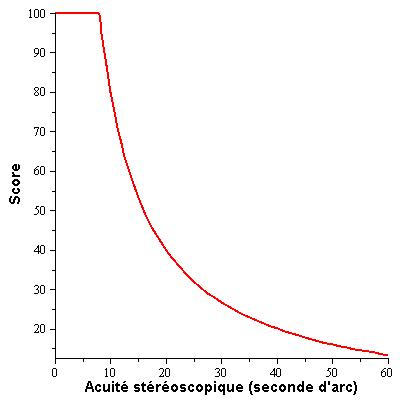
\includegraphics[scale=.75]{Figures/StereoAcuity}
		\caption{Tracé de la fonction de notation du critère <<~acuité stéréoscopique~>> ($\Delta \nu_{min} = 8~arcsecs$)}
		\label{fig:stereo_acuity}
	\end{figure}
		\chapter{Indices d'immersion}
\par Nous allons maintenant présenter les différents indices de la catégorie <<~immersion~>>. Ces indices sont fournis par l'environnement immersif et ne participent pas à la vision directement ; ils sont généralement issus du mouvement de l'utilisateur. Pour ces critères, les valeurs clefs sont plus difficilement trouvables dans la littérature: on verra donc que, dans un premier temps, certains critères sont simplifiés et nécessiteraient un travail plus approfondi.
	
	\section{Latence}
	\par La latence peut avoir différentes définitions, que nous verrons plus en détails dans la partie consacrée entièrement à la latence. Néanmoins, on propose en première approche les définitions suivantes, pratiquées dans l'industrie:
	\begin{itemize}
		\item <<~Mouvement à photon~>>: depuis le mouvement effectué par un utilisateur jusqu'à l'affichage de ce mouvement dans la simulation (que ce soit un mouvement de la tête avec un calcul de point de vue, ou le mouvement d'une autre partie du corps, suivant ce qui est surveillé). Peut être simplifié comme la latence <<~totale~>> du système et est la définition généralement utilisée.
		\item <<~Mouvement à pré-calcul~>>: le temps écoulé entre un mouvement tracké et l'ordre de recalcul de l'image à une nouvelle position. Plus simplement, c'est le temps d'acquisition des capteurs de mouvements.
		\item <<~Pré-calcul à calcul~>>: temps écoulé pour générer le rendu visuel, par le traitement informatique de toutes les informations.
		\item <<~Calcul à photon~>>: temps écoulé entre la fin du calcul de rendu et la fin de l'affichage sur l'écran. C'est le temps qui s'écoule entre l'ordre d'actualisation de l'image et la fin de la modification de tous les pixels.
	\end{itemize}
	
	\par Bien qu'il existe des mesures de seuil de perception de la latence dans la littérature \citep{brooks_whats_1999,kemeny_driving_2014} et des valeurs de latence humaine pour les images claires (74~ms) et pour les images sombres (106~ms) \citep{feng_han_investigation_2010}, on souhaite compléter ces informations. On met donc sur pied une expérimentation pour étudier ce phénomène en comparant son influence dans la réalisation d'une tâche de visée dans un CAVE et dans un casque.
	
	\section{Champ de regard}
	\par Le champ de regard (FOR - Field of Regard en anglais) est l'extension du champ de vision: il est défini comme la portion d'espace qui est visible, au cours du temps, en incluant la possibilité de bouger la tête (mais pas le corps) et les yeux dans leurs orbites. De même que précédemment pour le champ de vision, on élabore une fonction de score divisée en deux branches; la branche horizontale (H-FOR) et la branche verticale (V-FOR). Ces deux axes sont ensuite pondérés l'un par rapport à l'autre.
	
	\subsection{Champ horizontal \& champ vertical}
	\par En prenant en compte les mouvements possibles de la tête et des yeux (jusqu'à 15 degrés), chaque œil peut couvrir un champ de regard de plus de 200 degrés du côté temporal et d'environ 130 degrés du côté nasal, sur l'axe horizontal. L'axe vertical représente lui environ 310 degrés répartis à +140 et -170 d'après \citep{fuchs_traite_2003}.
	
	\par D'un côté, et parce que le champ visuel se recouvre, on limite la valeur maximale de H-FOR à 360 degrés ($h_{max}$). Le maximum de V-FOR est lui laissé tel quel à 310 degrés ($v_{max}$). De l'autre côté, les valeurs minimales ne peuvent pas être plus petites que les valeurs mesurées pour le champ de vision. On les nomme ici $h_0$ et $v_0$ mais ont les même valeurs que les $h$ et $v$ du champ de vision. L'évolution de la notation est linéaire pour chaque axe entre le minimum et le maximum.
	
	\par L'équation est donc (Eq. \ref{eq:field_of_regard_sub_items}), pour le champ de regard horizontal (H-FOR) et (V-FOR), avec $h$ et $v$ les valeurs mesurées des axes horizontaux et verticaux ; et $h_{0}$, $v_{0}$, $h_{max}$, $v_{max}$ défini précédemment pour le champ de vision:
	\begin{equation}
	\begin{cases}
		F_{H-FOR}(h) = \frac{100}{h_{max} - h_0} \cdot (h - h_0)\\
		F_{V-FOR}(v) = \frac{100}{v_{max} - v_0} \cdot (v - v_0)
	\end{cases}
	\label{eq:field_of_regard_sub_items}
	\end{equation}
	
	\subsection{Pondération}
	\par En faisant la même hypothèse que pour la pondération du champ de vision, on base les poids relatifs des deux axes sur leurs tailles respectives: 400 degrés pour l'axe horizontal et 310 pour l'axe vertical. Les 400 degrés de l'axe horizontal diffèrent des 360 utilisés pour la notation de l'axe (pour laquelle on avait limité l'angle à 360 degrés) et peuvent interpeller. Si mécaniquement lorsque que l'on regarde autour de soi on regarde à 360 degrés, dans les faits comme les demi-champs de regard (celui du côté temporal et celui du côté nasal) sont supérieurs à 180 degrés, on peut voir une petite partie de l'autre demi-champ de regard: une partie de l'espace est visible de deux manières (voir Fig. \ref{fig:demi_champs_regard}). En terme de possibilités donc le champ est plus grand que 360 degrés d'où la valeur de 400 degrés conservée. On utilise donc la même méthodologie que pour le champ de vision et on obtient (Eq. \ref{eq:field_of_regard_weighting}):
	\begin{equation}
	\begin{cases}
		k_h = \frac{400}{400 + 310} = 0.56\\
		k_v = 1 - k_h = 0.44
	\end{cases}
	\label{eq:field_of_regard_weighting}
	\end{equation}
	
	\begin{figure}[h]
		\centering
		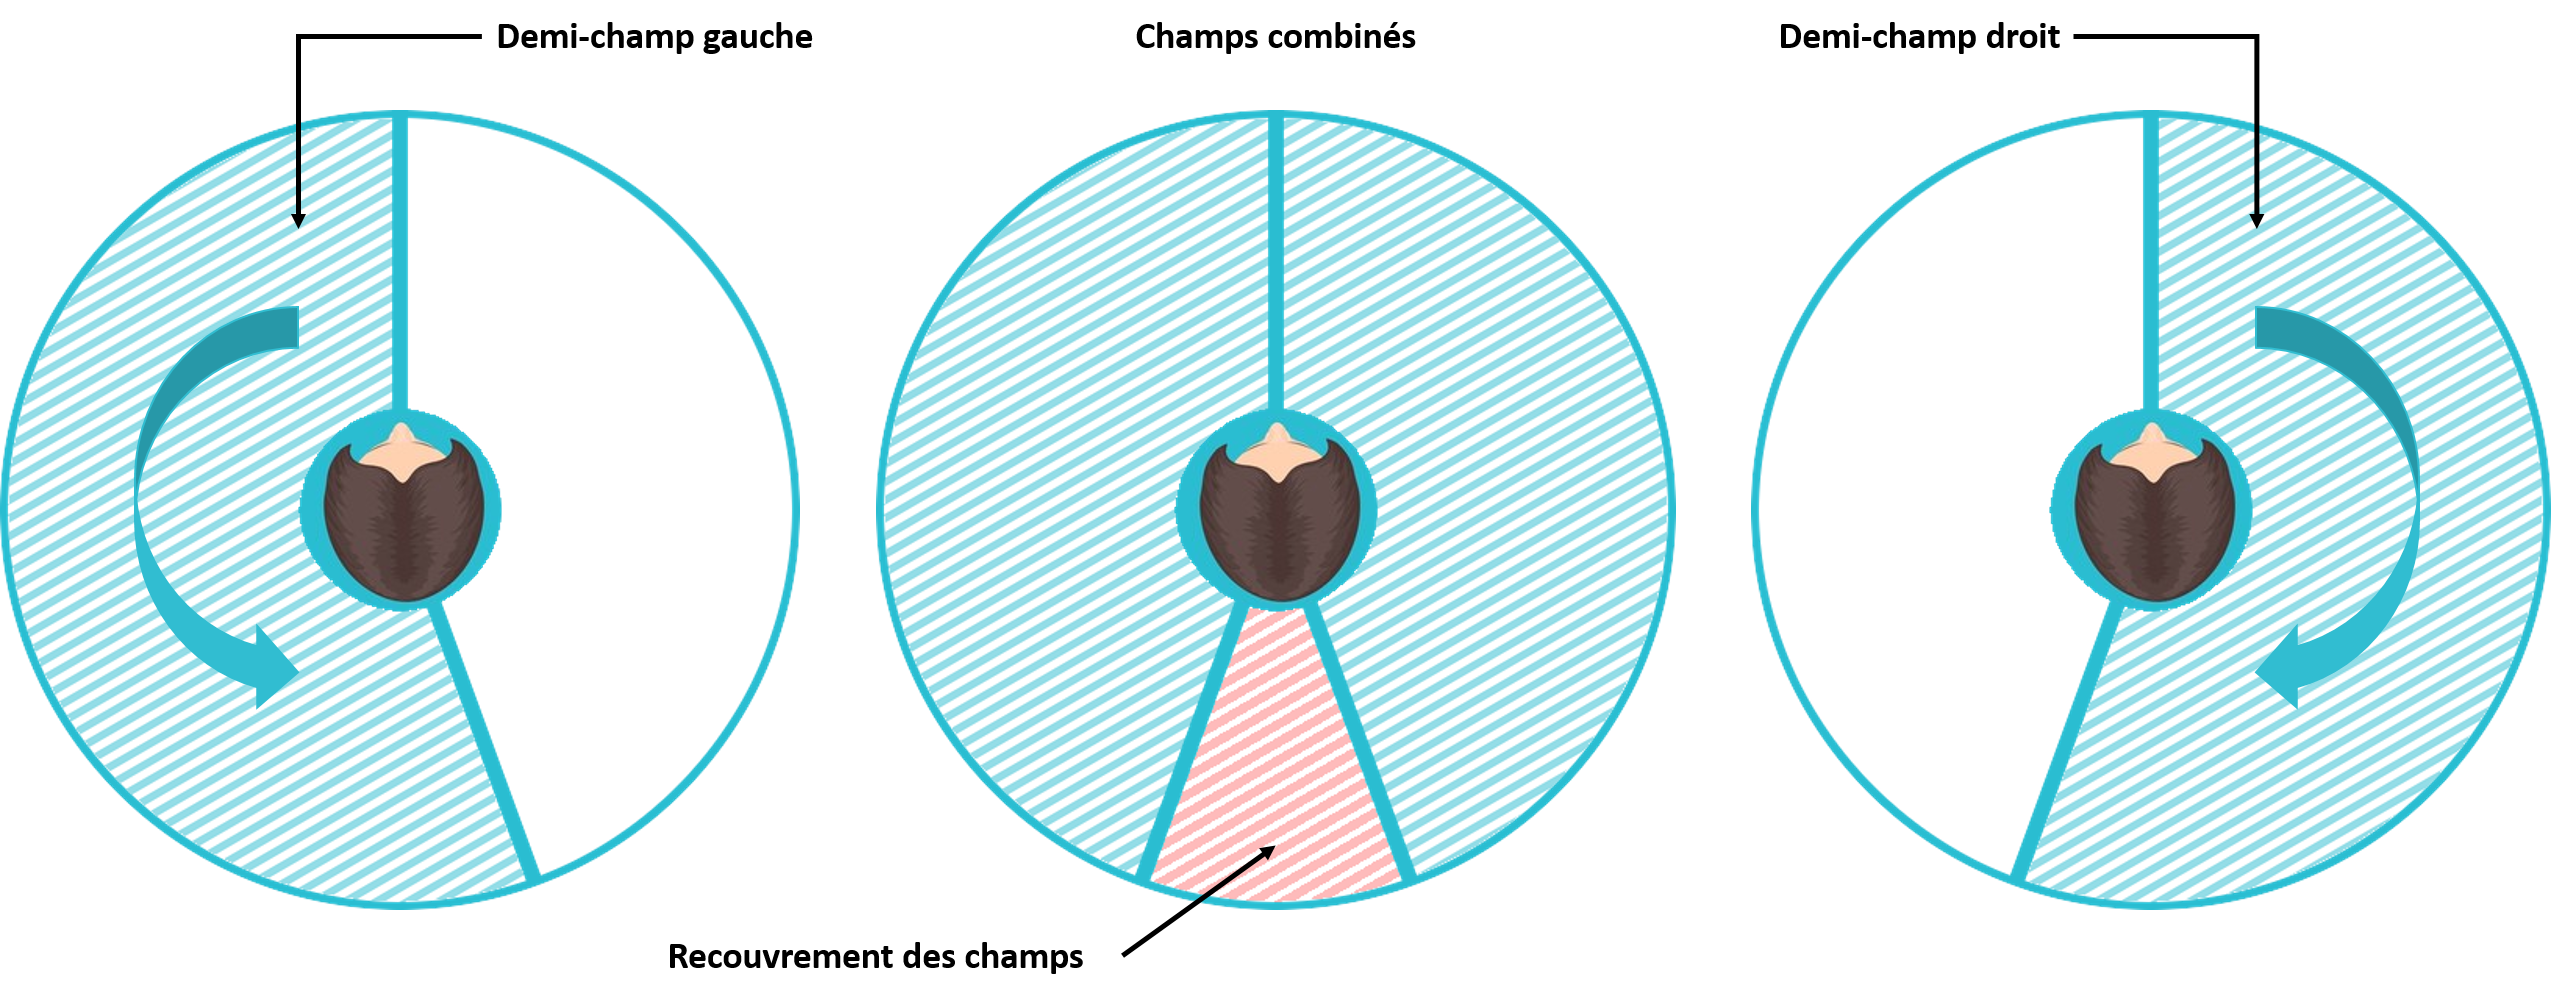
\includegraphics[scale=.35]{Figures/RecouvrementFOR}
		\caption{Recouvrement des demi-champs de regard (temporal et nasal).}
		\label{fig:demi_champs_regard}
	\end{figure}
	
	\par Ce qui est finalement assez proche de la pondération du champ de vision. Au final, la fonction de notation du champ de regard est définie par l'équation suivante (Eq. \ref{eq:score_field_of_regard}):
	\begin{equation}
	F_{FOR}(h,v) = k_h \cdot F_{H-FOR}(h) + k_v \cdot F_{V-FOR}(v)
	\label{eq:score_field_of_regard}
	\end{equation}
	
	\par Cette hypothèse de pondération est valable pour le cas général. On a vu par la suite, qu'elle pouvait être mise à mal dans certains cas de figures (voir chapitre sur l'expérimentation comparative entre les scores d'acceptation et les scores du modèle) et qu'il fallait, dans le cas par exemple d'une simulation de conduite, mettre la quasi intégralité de la pondération sur le champ de regard horizontal.
	
	\section{Stéréoscopie}
	\subsection{Fonctionnement}	
	\par La stéréoscopie est une méthode pour donner de la profondeur et du relief à des images  standard en 2D. Les yeux, de part leur écartement, ont des images d'un point de vue toujours différent. En combinant les informations (et notamment les différences entre les deux points de vue) le cerveau est capable de récréer la profondeur. Le principe de la stéréoscopie est donc de fournir à chaque œil une image différente, calculée avec le bon point de vue. Cela peut être réalisé via un certain nombre de techniques \citep{mehrabi_making_2013}. On se concentre dans notre cas sur les méthodes avec des lunettes portées (Casque, lunettes obturantes, lunettes polarisées, anaglyphes, ...). Ces dernières sont présentées par \cite{fauster_stereoscopic_2007}. On rappelle ici les deux techniques les plus connues (historiquement) pour amener du relief.
	
	\par Le type de stéréoscopie le plus connu du grand public est surement la technique dite <<~anaglyphe~>> qui fonctionne avec des lunettes aux verres rouge et bleu (voir Fig. \ref{fig:stereo_glasses}). Le principe est d'afficher les deux images nécessaires à la stéréoscopie en même temps mais chacune superposée par un filtre de couleur rouge ou de couleur bleue. Le verre rouge ne laisse passer que l'image rouge tandis que le filtre bleu ne laisse passer que son image de couleur correspondante. Chaque œil voit donc une seule image et le cerveau peut ainsi reconstruire la profondeur.
	
	\begin{figure}[h]
		\centering
		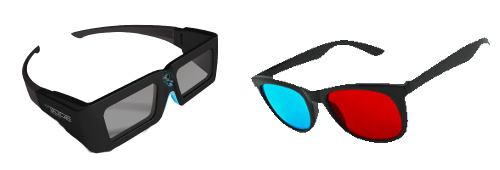
\includegraphics[scale=.8]{Figures/StereoActiveAnaglyphGlasses}
		\caption{Lunettes de stéréoscopie.}
		\label{fig:stereo_glasses}
	\end{figure}
	
	\par L'autre technique répandue est la stéréo dite <<~active~>> ; c'est celle utilisée par exemple dans les cinémas, mais surtout pour le cas qui nous occupe, dans l'industrie. Cette fois, les lunettes ont des filtres identiques et relativement transparents (voir Fig. \ref{fig:stereo_glasses}). Les images destinées aux yeux sont affichées l'une après l'autre (et pas en même temps comme la technique précédente) et ce sont les lunettes qui font le tri pour attribuer la bonne image au bon œil: de manière synchronisée avec l'affichage des images un verre devient opaque tandis que l'autre est transparent et ainsi de suite en alternance. Lorsque l'image pour l'œil gauche est affichée, le verre gauche laisse passer la lumière quand le verre droit la bloque, et inversement.
	
	\par Il existe aussi d'autres moyens de recréer une vision binoculaire comme les affichages auto-stéréoscopiques ou les affichages holographiques mais qui sortent du cadre d'étude car on se concentre sur les simulateur immersifs basés sur des techniques de stéréoscopie active. 
	
	\subsection{Fonction de notation du critère}
	\par En première approche, qui serait à étoffer, on propose de noter le critère sur sa présence (100) ou son absence (0). La piste d'amélioration à suivre pourrait être une découpe de la fonction de notation par rapport à la technique utilisée: toutes les techniques ne se valent pas et leurs performances pourraient être comparées. Il ne semble pas encore y avoir de telle comparaison dans la littérature. On propose en Fig. \ref{fig:stereo_grade_techno} un exemple à titre d'illustration uniquement.
	
	\begin{figure}[h]
		\centering
		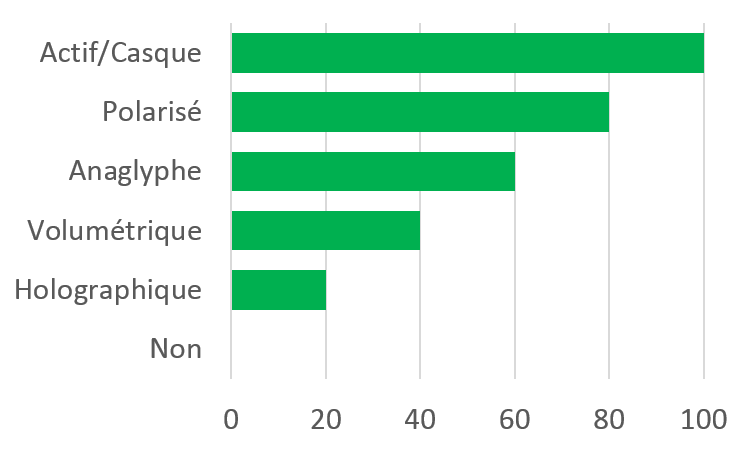
\includegraphics[scale=1]{Figures/StereoTechnoScore}
		\caption{Illustration d'une notation du critère <<~Stéréoscopie~>> en fonction de la technologie}
		\label{fig:stereo_grade_techno}
	\end{figure}
	
	\section{Tracking}
	\par Le tracking est surement un des éléments les plus importants pour l'immersion. Le tracking permet d'inclure les mouvements de l'utilisateur dans la simulation, que ce soit du corps ou de la tête, mais aussi l'inclusion d'appareils extérieurs ou autres. Là encore, il existe un grand nombre de techniques, que ce soit embarqué dans les casque de réalité virtuelle ou bien avec des solutions externes. Dans le cas d'un CAVE on utilise en général des caméras infrarouge et un système de boules réfléchissantes sur les objets (ou parties du corps) à repérer dans l'espace (voir Fig. \ref{fig:tracking_illustration}). Pour chaque objet dont on souhaite connaitre la position dans l'espace, on fixe au minimum trois boules réfléchissant les rayons infrarouges. Ces trois boules doivent être en permanence au même endroit sur l'objet et dans la même configuration (voir Fig. \ref{fig:tracking_illustration}, des deux côtés des lunettes). On balaye ensuite l'espace à tracker avec des caméras émettant et captant les rayons infrarouges. Le système de boules réfléchit ces rayons et est ainsi vu par les différentes caméras qui, comme elles sont placées à différents endroits dans l'espace, peuvent trianguler la position et l'orientation de l'objet étant donné que les boules réfléchissantes sont fixes par rapport à l'objet.
	
	\begin{figure}[h]
		\centering
		\includegraphics[scale=.6]{Figures/TrackingCameraBody}
		\caption{<<~Body~>> de tracking monté sur des lunettes de stéréoscopie \& ensemble caméra-émetteur infrarouge pour le tracking.}
		\label{fig:tracking_illustration}
	\end{figure}
	
	\par A défaut, et en attendant, de proposer une notation sur des critères plus développés, on propose de noter simplement ce critère sur sa présence (100) ou son absence (0). L'élément à creuser serait sa précision, c'est à dire son écart de position entre la position réelle de l'objet/body de tracking et la position vue par le système. Cette précision dépend néanmoins d'autres paramètres comme la calibration des caméras ou la calibration de la <<~room~>> (la définition des bordures de l'espace de travail). Il pourrait être aussi envisageable, au même titre que pour la stéréoscopie, de traiter le tracking en fonction de la technologie. Il faudrait alors comparer le tracking infrarouge avec le tracking magnétique ou autre.
		
	\section{Uniformité}
	\par Bien que défini dans le modèle, le critère d'uniformité est le seul qui n'a pas été pleinement abordé. C'est un sujet complexe qui se divise en plusieurs partie. L'uniformité peut à la fois valoir à l'intérieur d'un même écran, c'est à dire entre différentes zones d'un écran, mais aussi -quand le système le permet de part sa construction- entre les différents écrans. Même si l'uniformité la plus évidente concerne la couleur (on souhaite qu'un rouge affiché soit identique partout), il faut en fait l'élargir au d'autres critères:
	\begin{itemize}
		\item la couleur,
		\item la luminosité,
		\item le contraste.
	\end{itemize}
	
	\par La couleur est surement le critère le plus facile à vérifier car on sait mesurer des écarts entre les couleurs grâce aux équations de différentiations des couleurs (présentées dans la première partie du manuscrit). Ces équations donnent donc des écarts entre les couleurs qui, par construction doivent être inférieurs à une valeur de 1 pour qu'ils soient imperceptibles à l'oeil humain. Néanmoins, en informatique notamment, le seuil réel est plus bas (la valeur en dessous de laquelle la différence est imperceptible est plus grand que le 1 théorique) pour les population experte dans le domaine de la couleur, et encore plus bas pour les populations néophytes \citep{vidal_color-difference_2016}. On pourrait donc se baser sur ces trois valeurs (valeur théorique minimale, valeur de la population experte et valeur de la population néophyte) pour faire une première échelle de notation.
	
	\par Néanmoins, on présente ici les valeurs qui sont utilisées dans les cahiers des charges de Renault pour le design des moyens immersifs du groupe. Ces valeurs sont le fruit de l'expérience des ingénieurs et d'échanges avec les différents acteurs du milieu. Toutes les mesures sont faites selon la norme ANSI IT7.215, c'est à dire avec 9 points de mesure sur chaque écran. Ces points sont répartis en 3 lignes de 3: sur chaque ligne, un point centré encadré par deux autres points distants de 1/3 de la largeur totale de l'écran par rapport au bord.
	
	\par Pour la couleur, le mesures se font indépendamment sur du blanc uni et un gris 18\% uni (Gris RGB 128). Les spécifications sont à appliquer à la fois entre les différents points de mesure sur l'écran et à la fois entre les écrans, lorsque c'est le cas dans le système immersif. Dans le premier cas, le $\Delta E$ maximal toléré est de 6. Dans le deuxième cas, pour deux faces contiguës, seuls les 3 points les plus proches des bords en contact sont concernés. Un $\Delta E$ maximal de 6 est également requis.
	
	\par Pour la luminance, la différence entre le point le plus lumineux et le point le plus sombre ne doit pas dépasser 30\%, sur la base de la plus petite valeur mesurée. En cas d'écrans contigus, la différence entre le point le plus lumineux et le point le plus sombre ne doit pas dépasser 10\%, là encore sur la base de la plus petite valeur mesurée. De manière analogue aux spécifications sur la couleur, on n'utilise pas les 18 points de mesure mais seulement les 6 points les plus proches des bords comparés (3 par écran).
	
	\par Pour le contraste, la différence entre la valeur minimale et et la valeur maximale entre les différents écrans ne doit pas dépasser 25\% de la valeur minimale.
	
	\section{Orientation des caméras}	
	\subsection{Mimétisme du fonctionnement oculaire}	
	\par La capture d'image dans une scène virtuelle pour affichage sur un/des écran-s se fait au moyen d'une <<~caméra~>> virtuelle. Dans le cas de la stéréoscopie, comme il est nécessaire d'avoir une image par œil, deux caméras virtuelles entrent en jeu. Ces caméras sont l'équivalent virtuel de nos yeux. Il semblerait donc naturel que les caméras aient un comportement relativement proche de ces derniers et pourtant ce n'est majoritairement pas le cas.
	
	\par Lorsque l'on regarde un objet proche de nous, les yeux s'orientent dans leur orbite et se tournent vers cet objet. Plus l'objet est proche, plus il est nécessaire de converger. Au contraire, quand l'objet recule, et à partir d'une certaine distance, celui-ci est considéré comme <<~à l'infini~>> et les directions des yeux sont parallèles, soit avec une convergence nulle. Dans la majeure partie des cas, la convergence des caméras n'est pas implémentée: on parle alors de caméras <<~parallèles~>> (ou à <<~convergence~>> nulle). La raison vient du fait qu'utiliser des caméras arbitrairement convergées (et qui resteraient convergées, donc à <<~convergence fixe~>>) entraine automatiquement un certain nombre de distorsions \citep{woods_image_1993}. Si l'utilisateur regarde un objet à une <<~convergence~>> différente de celle qui est prévue, l'orientation des caméras n'est pas la bonne. Ainsi, plutôt par soucis de simplicité, on fait en général l'hypothèse que tous les objets (ou en tout cas la majorité) seront suffisamment éloignés pour être dans une situation de convergence nulle.
	
	\par Néanmoins on peut optimiser l'utilisation de ces distorsions si l'on est capable de régler la convergence des caméras en temps réel en fonction de la distance à laquelle l'utilisateur regarde. Cet ajout s'avère même bénéfique car il ajoute des disparités verticales qui font partie du processus de vision \citep{aurat_immersion_2016}. On peut alors parler de <<~caméras à convergence variable~>>. Il faut alors acquérir la position du regard en temps réel, ce qui peut être fait soit matériellement en ajoutant par exemple un système de tracking du regard (voir Fig. \ref{fig:eye_tracker}), soit en faisant des hypothèses telles que la personne regarde droit devant elle (et non en coin), donc la direction du regard est la même que la direction de la tête. La mise en œuvre de la convergence n'est également pas facilitée par le fait de capturer des images dans des plans non parallèles au plan de projection final. Les caméras convergées capturent des images planes mais dans un plan qui ne correspond par forcément à la surface sur laquelle il faudra la projeter (voir Fig. \ref{fig:redressement_plan_vision}). Il faut donc passer par une étape supplémentaire de warping de l'image \citep{aurat_immersion_2016}.
	
	\begin{figure}[h]
		\centering
		\includegraphics[scale=1]{Figures/EyeTrackerTobii}
		\caption{Exemple de système de tracking de regard portatif.}
		\label{fig:eye_tracker}
	\end{figure}
	
	\begin{figure}[h]
		\centering
		\includegraphics[scale=.75]{Figures/RedressementPlansVision}
		\caption{Exemple de déformation due à la convergence des caméras.}{Le carré est vu comme deux rectangles dans une configuration <<~caméras à convergence nulle~>> et comme deux trapèzes lorsque les caméras sont convergentes. Il faut donc retordre artificiellement les trapèzes pour qu'ils correspondent à la projection qui se fait sur une surface rectangulaire (image tirée de \citep{aurat_immersion_2016}).}
		\label{fig:redressement_plan_vision}
	\end{figure}
	
	\par Cette dichotomie entre la convergence réelle des yeux et la convergence artificielle des caméras virtuelles n'est pas anodine car elle est à l'origine d'un des plus grand maux dans les simulateurs: le conflit accommodation-vergence qui génère notamment des fatigues, fatigues visuelles, participe au mal du simulateur et dégrade grandement la qualité d'immersion \citep{neveu_impact_2012}. En effet, les images sont affichées sur un écran à une certaine distance auquel les yeux s'accommodent tandis que les images jaillissent (ou inversement, s'enfoncent) de l'écran, obligeant les yeux à converger dessus. L'accommodation et la convergence qui sont normalement liées sont dès lors désynchronisées et génèrent un conflit pour le cerveau.
	
	\subsection{Fonction de notation du critère}
	\par Ainsi, le critère est divisé en trois, soit le nombre de possibilité qui existent:
	\begin{itemize}
		\item caméras à convergence fixe (c'est à dire sans connaitre le point de regard), 0.
		\item caméras à convergence nulle (caméras parallèles), 80.
		\item caméras à convergence variable (avec connaissance du point de regard), 100.
	\end{itemize}
		\chapter{Pondération du modèle}
\par Il existe deux niveaux de pondération dans le modèle: un premier, local, à l'intérieur de certains critères (champ de vision et champ de regard), et un deuxième, global, qui donne un poids à chacun des critères les uns par rapport aux autres. On a déjà abordé la pondération locale et ses hypothèses, on s'intéresse ici au second niveau de pondération: au global.

\par La pondération complète du modèle est un travail conséquent qui nécessite un engagement entier. On ne prétend donc pas donner la solution mais simplement des propositions pour une première approche théorique.

\section{Contraste, luminance, taille et champs visuels}
\par Comme on a pu voir dans les chapitres précédents, la construction du modèle se base sur la vision et sa modélisation. Une première piste importante pour la pondération peut être relevée à l'étude du modèle de Rose \citep{rose_sensitivity_1948}, qui, on le rappelle, est décrit par une simple équation (Eq. \ref{eq:modèle_rose_2}):

\begin{equation}
	BC^2\alpha^2 = \text{constant}
	\label{eq:modèle_rose_2} 
\end{equation}

\par On voit clairement qu'une importance supérieure est attribuée aux critères de contraste et de taille par rapport au critère de luminance avec des puissances d'ordre 2 par rapport à une puissance d'ordre 1. On peut donc dire que le contraste et la taille de l'objet nécessite une pondération (plus) forte. Si on ne peut pas relier directement la taille de l'objet perçu à l'acuité visuelle, il est important de noter que plus l'acuité est forte, plus l'objet sera perçu finement. Enfin, par expérience, il nous semble même que le contraste est un critère capital et qu'il devrait recevoir la plus forte des pondérations.

\par La pondération (locale et globale) des champs de vision et de regard est fortement liée à l'application qui est faite dans le système immersif. On a pu le constater via une expérimentation qui sera décrite dans le chapitre suivant.

\begin{table}[h]	
	\centering
	\caption{Force relative des critères du modèle non liés à la perception de la profondeur}
	\label{tab:ponderation_non_profondeur}
	\small
	\begin{tabular}{lc}
		\multicolumn{1}{l}{\bfseries Paramètre} & \multicolumn{1}{c}{\bfseries Force relative}\\		
		Contraste & Fort\\
		Taille de l'objet & Fort\\
		Champ de vision & Variable\\
		Champ de regard & Variable\\
		Luminance & Faible\\
	\end{tabular}
\end{table}

\section{Tracking, stéréoscopie, convergence des caméras et couleurs}
\par Une autre piste très intéressante est issue de l'importance relative des indices de profondeur entre eux. On a déjà présenté les différents indices qui permettent au cerveau de reconstruire une carte de profondeur (voir la première partie sur l'état de l'Art). On s'intéresse ici à un classement par importance de ces indices.

\par Il existe quelques études qui ont comparé des indices de profondeurs entre eux afin de déterminer le(s)quel(s) est/sont prépondérant(s) sur les autres. Par exemple, \citep{mazur_relative_1990} compare la stéréoscopie avec la perspective aérienne et la comparaison de taille entre des objets familiers. \citep{reinhart_comparison_1990} ont comparé la taille relative des objets entre eux, la stéréoscopie (disparités binoculaires), l'interposition et la luminosité de l'objet, tandis que \citep{surdick_relevant_1994, surdick_perception_1997} comparent quant à eux 7 indices différents:

\begin{itemize}
	\item la luminance relative,
	\item la taille relative,
	\item la hauteur relative,
	\item la perspective linéaire,
	\item l'effet de rapprochement,
	\item le gradient de texture,
	\item la stéréoscopie.
\end{itemize}

\par Les résultats de \cite{mazur_relative_1990} et de \cite{surdick_relevant_1994} montrent une domination des indices de profondeur que sont la stéréoscopie, la perspective aérienne et la perspective linéaire. Les résultats de \cite{reinhart_comparison_1990} mettent en avant l'apport de la stéréoscopie par rapport aux indices monoculaires pour la perception de la profondeur de manière plus tranchée. On note néanmoins que la grande majorité des indices mis en concurrence sont des indices graphiques qui sont donc en dehors de notre cadre d'étude.

\par Parallèlement, \citep{mikkola_relative_2010} relèvent que la stéréoscopie et la parallaxe de mouvement sont considérées comme les indices les plus importants. Ces résultats sont à rapprocher de ceux de \citep{rogers_motion_1979} qui montrent que la parallaxe de mouvement est un indice de profondeur pertinent même lorsque tous les autres indices sont inexistants. \cite{mikkola_relative_2010} ont de leur côté conduit des expérimentations dans lesquelles ils demandaient à leurs sujets de noter de manière subjective l'impression de profondeur ressentie: la stéréoscopie arrive encore une fois avec de bon résultats tandis que des indices monoculaires tels que les ombres ou les textures des objets semblent avoir un impact plus réduit. 

\par Enfin, \citep{mehrabi_making_2013} ont réalisé des classifications sur les indices de profondeur, leurs atouts et leurs limitations (on trouvera une adaptation en Table \ref{tab:ponderation_depth_cues}) ainsi qu'une table sur les différentes techniques d'affichage en spécifiant notamment les indices de profondeurs disponibles dans chacun des cas. La classification est divisée en deux pondérations avec des indices ayant une contribution forte ou faible. Elle permet néanmoins déjà une bonne approximation pour un idée générale de pondération.

\begin{table}[h]	
	\centering
	\caption{Force relative des indices de perception de la profondeur. Table adaptée depuis \citep{mehrabi_making_2013}}
	\label{tab:ponderation_depth_cues}
	\small
	\begin{tabular}{lccc}
		\multicolumn{1}{c}{\bfseries Indice de profondeur} & \multicolumn{1}{c}{\bfseries Indice binoculaire} & \multicolumn{1}{c}{\bfseries Force relative} & \multicolumn{1}{c}{\bfseries Portée}\\		
		Parallaxe binoculaire & Oui & Fort & $2,5~m - 20~m$\\
		Parallaxe monoculaire & Non & Fort & $0 - \infty$\\
		Taille de l'image rétinienne & Non & Fort & $0 - \infty$\\
		Perspective linéaire & Non & Fort & $0 - \infty$\\
		Gradient de texture & Non & Fort & $0 - \infty$\\
		Recouvrement & Non & Fort & $0 - \infty$\\
		Accommodation & Non & Faible & $0 - 2~m$\\
		Convergence & Oui & Faible & $0 - 10~m$\\
		Perspective aérienne & Non & Faible & \textit{Long. dist. seulement}\\
		Ombrage & Non & Faible & $0 - \infty$\\
		Couleurs & Non & Faible & $0 - \infty$\\
	\end{tabular}
\end{table}

\section{Conclusion}
\par Il reste néanmoins des critères pour lesquels la littérature ne donne pas immédiatement un a priori de pondération tels que le nombre d'images par seconde, la latence ou l'uniformité entre les écrans. Par défaut (à l'exception de la latence qui par expérience est un indice très fort) on leur attribue une importance relative plus faible que les facteurs <<~forts~>> qui semblent très prépondérants sur les autres.

\par On a maintenant une meilleure idée générale des tendances qu'il peut exister pour une pondération du modèle dans le cas général. Dans des cas spécifiques (voir chapitre suivant) comme la conduite, la pondération peut fortement varier en fonction des besoins de l'utilisateur. On présente ces ordres de grandeur en Fig. \ref{fig:modèle_définitif_pondere} en modélisant les pondérations <<~fortes~>> avec une boite plus grande que les pondérations <<~faibles~>>.

\par Il convient de rappeler que cette proposition est une ébauche et que la définition précise d'une (ou de plusieurs) pondération(s) reste un sujet à part entière que nous n'avons pas, à proprement parler, traité.

\begin{figure}
	\centering
	\includegraphics[scale=1]{Figures/ModeleDefinitifPondere}
	\caption{Modélisation avec ordre de grandeur de la pondération.}
	\label{fig:modèle_définitif_pondere}
\end{figure}
		\chapter{Etude expérimentale}
\label{chap:sdr_etude_experimentale}
	\section{Objectif}
		\par On a réalisé une expérimentation pour comparer les notes données par notre modèle de score et les notes données par des utilisateurs d'un système d'affichage immersif aux différentes caractéristiques que l'on retrouve dans le modèle: fluidité, couleurs, contraste, ... Cette expérimentation n'a pas pour but -et ne peut pas- valider notre modèle: elle compare deux types de données très différentes, les unes objectives et les autres subjectives. C'est seulement une comparaison entre un modèle théorique qui donne un score qui reflète à quel point la partie hardware du système donne un signal proche de celui défini dans les modèles de vision, et un score donné subjectivement par les sujets et qui reflète à quel point les utilisateurs ont apprécié les différentes capacités du système.
		
		\par Cependant, cette expérimentation nous permet de montrer la différence qui peut exister entre l'appréciation d'un critère noté subjectivement et sa note de performance théorique. Cela nous permet aussi de récupérer des indices sur la manière dont les utilisateurs se comportent dans un système immersif et dans le cas spécifique de cette simulation ; ces indices nous aideront ensuite dans certaines de nos hypothèses.
		
	\section{Apparatus}
	\par 32 sujet ont été réunis pour cette expérimentation: 23 hommes et 9 femmes, âgés de 20 à 27 ans, avec une moyenne d'âge de 25 ans (écart-type: 1,8 ans). Elle a été faite dans un CAVE 4 faces dont les dimensions sont présentées en Tab. \ref{tab:cave_dimensions}. La taille des pixels était de $2,25~mm$ et les sujets étaient assis de manière à avoir les yeux à 2~m de l'écran de face. L'expérimentation était écologique: les sujets devaient simplement conduire dans le simulateur. La conduite était faite au moyen d'un ensemble Logitech G25 avec volant et pédales, le tout connecté au logiciel de simulation SCANeR Studio\footnote{\url{http://www.oktal.fr/en/automotive/range-of-simulators/software} (lien raccourci: \url{https://lc.cx/NxyR})}. Les sujets étaient assis dans un vrai siège de voiture posé au sol. L'environnement virtuel de simulation était un simple paysage avec une route en boucle fermée mêlant à la fois mer, bord de lac, ville et montagne.
	 
	\begin{table}[h]
		\centering
		\caption{Dimensions du CAVE <<~P3I~>>}{Lieu de l'étude expérimentale sur la comparaison entre les notes objectives et des notes subjectives.}
		\label{tab:cave_dimensions}
		\small
		\begin{tabular}{ccc}
			\multicolumn{1}{c}{\bfseries Face} & \multicolumn{1}{c}{\bfseries Taille} & \multicolumn{1}{c}{\bfseries Résolution}\\
			Avant & 3.60 x 2.70 m & 1600 x 1200 px\\
			Gauche & 4.20 x 2.70 m & 1920 x 1200 px\\
			Droite & 4.20 x 2.70 m & 1920 x 1200 px\\
			Sol & 4.20 x 3.60 m & 1600 x 1200 px\\
		\end{tabular}
	\end{table}
	 
	 \par Chaque sujet devait faire la même chose: conduire pendant 8 minutes sans autre tâche particulière que de regarder tout autour de soi. La vitesse de la voiture était limitée à 30km/h, et ce, pour plusieurs raisons: rester dans le même cas d'usage en basse vitesse pour tout le monde et ne pas rendre malade les sujets. Après les 8 minutes de conduite, les sujets devaient noter via une échelle <<~aidée~>> de 1 à 5 (voir Fig. \ref{fig:aided_scale}) les différents critères de notre modèle, par comparaison à ce qu'ils pourraient voir en situation réelle.
	 
	 \par Une comparaison a ensuite été faite entre les moyennes des notes subjectives des sujets et les valeurs théoriques objectives du modèle de score. Aucune pondération n'était appliquée sur les critères (mis à part les pondérations internes aux critères de champ de vision et de champ de regard).
	
	\begin{figure}[h]
		\centering
		\includegraphics[scale=1]{Figures/AidedScale}
		\caption{Echelle <<~aidée~>> pour noter subjectivement de 1 à 5 les différents critères du système}
		\label{fig:aided_scale}
	\end{figure}
	
	\par Pour représenter la variation de taille, et donc de hauteur des yeux par rapport au sol en position assise entre les différents sujets, les valeurs théoriques de champ de vision et de champ de regard sont calculées deux fois avec $1,10~m$ et $1,15~m$ de hauteur d'yeux (par rapport au sol, en position assise sur le siège de conduite). On moyenne ensuite ces deux valeurs.
	
	\par On a sélectionné seulement des sujets jeunes (de 20 à 27 ans) et dont la vision était théoriquement parfaite (ou corrigée pour être parfaite). Cela a été fait afin de rester sur des sujets dont les capacités de vision (vision du contraste, de la luminance, acuité, ...) n'ont pas commencé à décroitre en fonction de l'âge, processus qui commence autour de 30 ans.
	
	\section{Résultats}
	\par Afin d'analyser les résultats, la population de sujets a été divisée en 8 sous-catégories. Les caractéristiques de ces différentes sous-catégories peuvent être trouvées dans la Table \ref{tab:subpopulations}. Aucun résultat statistique ne peut être tiré de la catégorie <<~femme + gamer~>> puisque qu'elle ne comporte qu'un seul membre.
	
	\begin{table}[h]
		\centering
		\caption{Population et âge des sous-catégories de l'étude expérimentale sur la comparaison entre les notes objectives et des notes subjectives.}
		\label{tab:subpopulations}
		\small
		\begin{tabular}{lccc}
			\multicolumn{1}{c}{\bfseries Sous-catégorie} & \multicolumn{1}{c}{\bfseries Population} & \multicolumn{1}{c}{\bfseries Âge moyen} & \multicolumn{1}{c}{\bfseries Écart-Type}\\
			Total & 32 & 24.8 ans & 1.8\\			
			Hommes (M) & 23 & 24.8 ans & 2\\
			Femmes (W) & 9 & 24.8 ans & 1.7\\
			Gamers (G) & 13 & 24.5 ans & 2.3\\
			Non gamers (NG) & 19 & 25 ans & 1.5\\
			M+G & 12 & 24.7 ans & 2.3\\
			M+NG & 11 & 24.9 ans & 1.6\\
			W+G & 1 & 22 ans & 0\\
			W+NG & 8 & 25.1 ans & 1.5\\
		\end{tabular}
	\end{table}
	
	\par Cinq valeurs théoriques du modèle étaient assez mûres pour être calculées et être comparées aux notes données par les sujets:
	\begin{itemize}
		\item le nombre d'images par seconde
		\item les couleurs
		\item l'acuité monoscopique
		\item le champ de vision
		\item le champ de regard
	\end{itemize}		
	
	\par Les autres critères n'étaient soit pas encore notables via le modèle de score (luminance, contraste, latence et uniformité) soit difficiles à noter par un simple questionnaire sans procéder pendant l'expérimentation à une tâche particulière mettant en avant la caractéristique (acuité stéréoscopique, tracking et stéréoscopie).
	
	\par Les valeurs des moyennes et des écarts types des cinq critères retenus pour cette étude expérimentale sont données en Fig. \ref{fig:results_comparison}.
	
	\begin{figure}[h]
		\centering
		\includegraphics[scale=.7]{Figures/ResultsComparison}
		\caption{Résultats des valeurs théoriques calculées et des valeurs subjectives relevées sur l'ensemble de la population des sujets.}
		\label{fig:results_comparison}
	\end{figure}
	
	\section{Discussion}
	\par Les résultats de la comparaison entre le modèle théorique et l'acceptation psychologique par les sujets peuvent être divisés en trois catégories. Premièrement les valeurs relevées sur les questionnaires correspondent plutôt bien aux valeurs données par le score théorique. C'est le cas par exemple pour le critère <<~images par seconde~>>.
	
	\par Deuxièmement, et en opposition à la première catégorie de résultats, deux critères diffèrent fortement par rapport aux valeurs d'acceptation par les sujets: dans un sens (pour les <<~couleurs~>> les valeurs subjectives sont supérieures aux valeurs objectives) comme dans l'autre (pour l'<<~acuité monoscopique~>> les valeurs théoriques sont supérieures aux valeurs d'acceptation).
	
	\par Enfin, la troisième catégorie contient des critères qui ont des valeurs objectives très différentes (96,95 pour le  <<~Champ de Vision~>> et un pauvre 38,50 pour le <<~Champ de Regard~>>) mais qui ont pourtant des valeurs subjectives très proches l'une de l'autre.   
	
	\subsection{Couleurs et acuité monoscopique}
	\par Ces deux critères montrent une grande différence de notation entre leur score théorique et leur score subjectif même si, à l'intérieur des sous-catégories, les moyennes et les écarts-type sont assez proches.
	
	\par D'un côté, les sujets étaient globalement satisfaits de la quantité de couleurs bien que ce soit en fait assez peu par rapport à toutes les couleurs visibles réellement. Une raison possible à cette divergence est l'absence de référence au monde réel pour juger par comparaison et l'utilisation usuelle massive d'appareils utilisant le même espace limité de couleurs (smartphones, télévisions, cinéma, ...).
	
	\par De l'autre côté, l'acuité monoscopique n'a pas été bien notée alors qu'elle aurait dû paraitre suffisante. On peut l'expliquer aussi par l'habitude d'avoir une très forte demande sur la résolution des écrans, que ce soit pour les téléphones, les ordinateurs ou les écrans divers.
	
	\subsection{Champ de vision \& champ de regard}
	\par Bien que légèrement plus élevée, la valeur théorique du champ de vision est assez proche de sa valeur d'acceptation associée et est, en plus, contenue dans la majorité des écarts-type des sous catégories. Cependant, la valeur théorique du champ de regard est extrêmement basse comparée à sa valeur d'acceptation et éloignée de tous les écarts-type des sous-populations.
	
	\par La valeur théorique basse vient du fait que, même si l'angle de vision horizontal est très bon, il n'y a pas de face supérieure d'affichage dans le CAVE, ce qui joue très négativement dans la notation de l'axe vertical du critère. A cause de la pondération quasi équivalente pour les deux axes, la note globale du critère est tirée vers le bas par la partie verticale qui est très basse.
	
	\par La tâche de conduite nécessite la quasi totalité de l'attention du conducteur à l'avant de la voiture et implique majoritairement l'axe horizontal de la vision. C'est pourquoi les sujets n'ont pas eu besoin d'utiliser particulièrement d'autres écrans que celui face à eux ni besoin d'images qui seraient hors-écrans. Cela peut expliquer pourquoi les participants ont noté le champ de regard si proche du champ de vision, car ils ont rarement dépassé les bornes du champ de vision et, quand c'était le cas, seulement un petit peu. Cela implique, dans ce cas précis, que notre hypothèse de pondération des axes en fonction de leur taille respective n'est pas correcte. Un jeu de pondération spécifique à la conduite devrait être calculé et appliqué, limitant considérablement l'influence de l'axe vertical.
	
	\par Enfin, on remarque une tendance intéressante à mettre en avant (bien que non soutenue par une preuve statistique). Les femmes (joueuses ou non) semblent être plus sévères dans leur notation que les hommes, et ce, quelle que soit la note théorique associée.
		\chapter*{Conclusion}
\addcontentsline{toc}{chapter}{Conclusion}
\markboth{CONCLUSION}{}
\par La première approche de la thèse, développer un <<~modèle de vision~>> traduit pour la Réalité Virtuelle, s'est vite révélée être une impasse. On choisit alors une approche différente: plutôt que de <<~faire~>> du réalisme, il pourrait être intéressant de <<~quantifier~>> le réalisme. A notre connaissance, il existe peu voire très peu de modèles ayant pour but de quantifier objectivement le réalisme physiologique dans la littérature.

\par On propose alors une évaluation de la performance d'un système via un score basé sur le système visuel humain qui dépeindrait, pour un système immersif donné et pour une situation donnée, à quel point le simulateur est efficace pour transmettre le bon niveau d'informations visuelles et, étant dans un système de Réalité Virtuelle, le bon niveau d'indices d'immersion. Ce score est en fait la réunion de douze critères chacun lié à une caractéristique de la vision et/ou de l'immersion visuelle (c'est à dire les critères immersifs dérivés directement du système visuel ou du système en lui-même). Chaque critère est jugé indépendamment puis contribue à la note globale via une pondération. La notation en elle même se fait, principalement, basée sur la littérature. Si on a pu appliquer cette méthode pour la majorité des cas, certains critères ne se prêtent pas à un tel traitement et ont bénéficié d'une notation particulière.

\par Les critères sont répertoriés en deux sections:
	
\begin{itemize}\itemsep12pt
	\item \textbf{Indices de vision:} contraste et luminosité (luminance), images par seconde, nombre de couleurs affichables, champ de vision, acuités monoscopique et stéréoscopique.
	\item \textbf{Indices d'immersion:} latence, champ de regard, stéréoscopie, tracking, uniformité et convergence des caméras.
\end{itemize}
	
\par Après une étude théorique fouillée pour déterminer la plus grande majorité des critères, on a réalisé une expérimentation pour comparer les notes données par notre modèle de score et les notes données par des utilisateur. Cette expérimentation n'avait pas pour but -et ne peut pas- valider notre modèle mais elle nous a permis de montrer la différence qu'il peut exister entre l'appréciation d'un critère noté subjectivement et sa note de performance théorique.

\par Néanmoins, il reste des points à développer. Certains critères ne sont pas aboutis et doivent être complétés par la pratique. C'est le cas par exemple du contraste et de la luminance, ainsi que de la latence. Le traitement expérimental de ces critères sera abordé dans les deux prochaines parties. Enfin, même si on a pu rapidement aborder la pondération intra-critère (champ de vision et champ de regard) ainsi que la légitimité des hypothèses sur lesquelles elle est construite (étude expérimentale), il restera encore tout un travail autour de la pondération inter-critères. Le sujet est extrêmement vaste et complexe car il dépend fortement de ce que l'on fait dans le système immersif.

\par Nous allons maintenant présenter le travail d'expérimentation qui a été réalisé autour de la validation du modèle de Rea en Réalité Virtuelle, pour le critère <<~contraste - luminance~>>.
	\part{Partie expérimentale: contraste et luminance}

\chapter*{Introduction}
\addcontentsline{toc}{chapter}{Introduction}
\markboth{INTRODUCTION}{}
\par Dans le chapitre précédent, on a décrit deux approches possibles pour le critère de contraste et de luminance: les fonctions de sensibilité au contraste et la performance visuelle relative. On s'intéresse ici au concept de performance visuelle. On en a présenté les deux principales modélisations: le modèle de Blackwell et de la CIE \citep{blackwell_ieri:_1971}, puissant mais hermétique, et le modèle de Rea et ses évolutions \citep{rea_toward_1986}. On a également pointé le fait que ces modèles, bien qu'intéressants, n'étaient pas à l'origine conçus pour la réalité virtuelle et nécessitaient donc une vérification expérimentale.

\par Il a été nécessaire de choisir entre les deux modèles, celui de Rea et celui de la CIE et Blackwell. Le modèle de Blackwell semble plus complet avec une portée d'action comprise en $1$ et $10000~cd/m^2$ et un calcul basé sur trois processus de vision, décrits comme principaux, impliqués dans la reconnaissance des détails de la tache à effectuer, dans le maintient des yeux en position fixe pendant les périodes de fixation, et enfin, dans la réalisation de mouvements rapide des yeux (les saccades). Néanmoins, le modèle de la CIE est une boite noire générée à partir de la mise en commun des travaux d'un certain nombre de chercheurs. Il n'existe pas d'expérimentation détaillée qui puisse être refaite, et à fortiori, encore moins en réalité virtuelle.

\par De l'autre côté, la modèle de Rea est plus limité en portée (entre $12$ et $169~cd/m^2$) mais présente en détail tout le protocole qui a été mis en œuvre pour développer les équations de performance visuelle. De plus, l'intervalle de fonctionnement du modèle correspond relativement bien aux luminances atteignables dans un simulateur et n'est donc pas très contraignant.

\par L'objectif de cette partie est donc de vérifier par l'expérimentation, dans un simulateur, les prédictions de performance du modèle de Rea. Pour ce faire, on a transposé en Réalité Virtuelle l'une des expérimentations mise en place par Rea et Ouellette pour déterminer leur modèle.
		\chapter{Modèles de Rea}
	\section{Première modélisation de la performance visuelle relative}
	\par Les sections suivantes décrivent brièvement le contexte et les premiers travaux de Rea qui l'ont mené à proposer sa propre modélisation de la performance visuelle \citep{rea_toward_1986, rea_toward_1987}, définie comme étant la vitesse et la précision atteintes pendant la réalisation d'une tâche visuelle.
	
	\subsection{Modèle précurseur}	
	\par Le premier modèle de Rea est directement inspiré de l'effet de compression proposé par \cite{naka_attempt_1966} qui modélise qu'à partir d'un certain niveau d'intensité, lorsque l'intensité du stimulus augmente, la réponse sensorielle associée augmente de moins en moins jusqu'à atteindre une forme de plateau (voir Fig. \ref{fig:compression_effect}). Les différentes courbes représentent les longueurs d'onde des lumières de couleur utilisées. Cet effet est modélisé de la manière suivante: $\frac{R}{R_{max}} = \frac{I^n}{I^n + k^n}$.
	
	\par Dans cette équation, le rapport de la réponse sensorielle ($R$) sur la réponse sensorielle maximale ($R_{max}$) est égal au rapport de l'intensité $I$ montée à une puissance $n$ déterminée sur la somme de cette même intensité $I$ montée à la puissance $n$ et d'une intensité $k$, également montée à la puissance $n$. La réponse à l'intensité $k$ est égale à la moitié de la réponse sensorielle maximale: $R(k) = \frac{R_{max}}{2}$.
	
	\par On peut faire l'analogie suivante pour donner un bon exemple de l'effet de compression: si dans une pièce on allume une deuxième ampoule d'égale intensité, la sensation de luminosité va grandement augmenter. Au contraire, si on rajoute une ampoule dans une pièce dans laquelle déjà mille ampoules sont allumées, la différence de luminosité perçue sera minime.	
	
	\begin{figure}[h]
		\centering
		\includegraphics[scale=.6]{Figures/CompressionEffect}
		\caption{Illustration de l'effet de compression.}{Image tirée de \citep{naka_attempt_1966}}
		\label{fig:compression_effect}
	\end{figure} 
	
	\subsection{Application à la performance visuelle}
	\par Rea s'est imposé deux règles pour la conception de son modèle: la performance visuelle doit être issue d'une performance à la réalisation d'une tâche, et le modèle doit être cohérent avec la littérature, notamment avec l'effet de compression que l'on vient de décrire.
	
	\par Le stimulus est décrit (Eq. \ref{eq:rea_contraste}) comme la différence entre le seuil de contraste $C_t$, calculé avec la formule de Blackwell (Eq. \ref{eq:rea_contraste_blackwell}), qui représente le contraste minimal à partir duquel la perception devient possible en fonction de la luminosité du fond ($L_B$) et le contraste visuel $C_V$ qui correspond au contraste entre la luminosité du fond et la luminosité de la tache visuelle ($L_T$) (Eq. \ref{eq:rea_contraste_blackwell}).
	
	\begin{equation}
		C_t = 0.048\left[\left(\frac{0.308}{L_B}\right)^{0.4} + 1.0\right]^{2.5}
		\label{eq:rea_contraste_blackwell}
	\end{equation}
	
	\begin{equation}
		C_V = \frac{L_B - L_T}{L_B}
		\label{eq:rea_contraste_visuel}
	\end{equation}
	
	\begin{equation}
		\Delta C = C_V - C_t
		\label{eq:rea_contraste}
	\end{equation}
	
	\par Les calculs suivants sont ensuite tirés de régressions polynomiales de degré 2 faites avec leurs données expérimentales:
	
	\begin{equation}
		\begin{cases}
		n =  0.882 + 4.38 \theta_1 - 6.05 \theta_1^2\\
		\theta_1 = \log(\log(L_B))
		\end{cases} 
		\label{eq:rea_n}
	\end{equation}
	
	\begin{equation}
		\begin{cases}
		k =  -2.25 + 1.77 \theta_2 - 0.217 \theta_2^2\\
		\theta_2 = \log(L_B)
		\end{cases} 
		\label{eq:rea_k}
	\end{equation}
	
	\begin{equation}
		VP_{max} = 0.0628 + 0.0120 \theta_2 - 0.00268 \theta_2^2
		\label{eq:rea_vpmax}
	\end{equation}
	
	\par Au final, la performance visuelle s'écrit de la manière suivante (Eq. \ref{eq:rea_perfrmance_visuelle}):
	\begin{equation}
		VP = \frac{(\Delta C)^n}{(\Delta C)^n + (k/L_B)^n}
		\label{eq:rea_perfrmance_visuelle}
	\end{equation}
	
	\par Et $RVP = \frac{VP}{f}$ avec $f$ la valeur de $VP_{max}$ dans les meilleurs conditions (luminance et contraste maximaux). Dans le cas de l'expérimentation de Rea, $f = 0.076$.
	
	\par Les résultats de cette expérimentation permettent à l'auteur de dégager trois tendances:
	\begin{itemize}
		\item A contraste constant, la performance augmente avec la luminance,
		\item La performance augmente plus rapidement avec le contraste lorsque les conditions de luminance sont plus élevées,
		\item La performance varie assez peu entre des conditions moyenne et supérieure de contraste.
	\end{itemize}
	
	\section{Méthode des temps de réaction}
	\par Rea et Ouellette complètent la démarche initiale de Rea en proposant une méthode pour établir la performance visuelle d'un sujet, basée sur la mesure et la prédiction des temps de réaction de ce dernier à l'apparition d'un stimulus visuel calibré \citep{rea_visual_1988, rea_relative_1991}. C'est cette modélisation que l'on va chercher à traduire en réalité virtuelle afin de déterminer si elle est utilisable dans le cadre de notre score de réalisme, pour le critère de contraste et de luminance.
	
	\subsection{Protocole expérimental}
	\par L'objectif était de mesurer le temps de réaction de sujets à l'apparition d'une cible sur un écran. La couleur de la cible était calibrée pour obtenir un contraste choisi par rapport au fond sur lequel elle était affichée.
	
	\par L'expérimentation était découpée en deux parties: une première série de mesures pour des cibles plus foncées que le fond sur lequel elles étaient présentées (méthode décrémentale) puis une autre série de mesures avec des cibles plus claires que le fond de présentation (méthode incrémentale).
	
	\par Les cibles, un carré, étaient présentées à $1.68~m$ de l'œil du sujet sur un écran occupant 12 degrés de champ de vision horizontal et 7 degrés de champ de vision vertical. Toutes les cibles étaient vues avec l'œil gauche, à travers un filtre neutre réglable et avec l'ajout d'un voile lumineux artificiel directement au niveau de l'œil (Fig. \ref{fig:rea_apparatus}).
	
	\begin{figure}[h]
		\centering
		\includegraphics[scale=.75]{Figures/ReactionTimeApparatus}
		\caption{Installation de l'expérimentation de Rea et Ouellette.}{Image tirée de \citep{rea_visual_1988}}
		\label{fig:rea_apparatus}
	\end{figure}
	
	\par Le contraste du carré était calculé en utilisant l'équation suivante (Eq. \ref{eq:rea_ouellette_contraste}):
	 \begin{equation}
		C = \frac{\vert (T L_b + L_v) - (T L_t + L_v) \vert}{T L_b + L_v} = \frac{T \vert L_b - L_t \vert}{L_a}
		\label{eq:rea_ouellette_contraste}
	\end{equation}
	
	\par Avec $T$ la valeur de transmittance du filtre (entre 0 et 1), $L_b$ la luminance du fond de l'écran, $L_t$ la luminance du carré à détecter et $L_v$ la luminance de voile ajoutée artificiellement. $L_a$ représente quant à elle la valeur de la luminance d'adaptation, c'est à dire la valeur pour laquelle l'œil et tout le système optique sont réglés (avec par exemple l'adaptation du diamètre pupillaire).
	
	\par Chaque apparition de cible était espacée d'une temporisation de 1.5 secondes puis d'une temporisation aléatoire variant entre 1 et 3 secondes. La taille de la tache visuelle était variable entre $0.20$ et $280 \times 10^{-5}~steradians$\footnote{Unité sans dimension. un angle solide d'un stéradian délimite sur la sphère unité à partir du centre de cette sphère une surface d'aire 1.}.
	
	\par Chaque sujet a enregistré $19200$ mesures de temps de réaction pour la partie décrémentale et $3625$ mesures pour la partie incrémentale.
	
	\subsection{Calcul des temps de réaction théoriques}
	\par Une fois toutes les mesures effectuées, cela a permis de réétablir une équation de performance avec une protocole similaire à la première modélisation et décrit plus haut. Le détail de ces calculs est présenté en annexe et on retiendra ici seulement l'équation suivante (Eq. \ref{eq:rea_ouellette_performance}):
	\begin{equation}
		R = \frac{(\Delta C_d)^{0.97}}{(\Delta C_d)^{0.97} + K^{0.97}}
		\label{eq:rea_ouellette_performance}
	\end{equation}
	
	\par De cette équation qui décrit la performance du sujet à détecter l'apparition de la tache visuelle en fonction des conditions d'illumination et de contraste, on dérive le temps de réaction en prenant simplement l'inverse de la performance (Eq. \ref{eq:rea_ouellette_reaction_time}):
	\begin{equation}
		RT = \frac{1}{R}
		\label{eq:rea_ouellette_reaction_time}
	\end{equation}
	
	\par Cela permet d'avoir un comportement logique dans les résultats avec un temps de réaction qui diminue quand la performance augmente et inversement.
	
	\par De plus, cette performance $R$ liée au temps de réaction, ainsi calculée, peut être reliée au modèle initial de performance visuelle relative. Cela nécessite d'appliquer deux opérations sur l'ensemble des résultats mesurés dans les deux expérimentations pour les mêmes conditions d'illumination, de contraste et de taille de cible: le calcul de $\Delta T_{vis}$: la variation du temps de réaction par rapport au temps obtenu dans les meilleures conditions expérimentales (Eq. \ref{eq:rea_ouellette_delta_t_vis}). Vient ensuite une transformation linéaire (Eq. \ref{eq:rea_ouellette_linear_transformation}):
	\begin{equation}
		\Delta T_{vis} = RT_{ref} - RT
		\label{eq:rea_ouellette_delta_t_vis}
	\end{equation}
	
	\begin{equation}
		RVP = RVP' \left(\frac{Delta T_{vis} - Delta T_{vis,r}}{Delta T_{vis}' - Delta T_{vis,r}}\right)
		\label{eq:rea_ouellette_linear_transformation}
	\end{equation}
	
	\par Avec $RT_{ref}$ le temps de réaction <<~étalon~>> obtenu dans les meilleures conditions expérimentales, $RVP'$ la valeur maximale de performance visuelle pour le jeu commun de conditions expérimentales, $\Delta T_{vis}'$ la meilleure valeur pour le jeu commun et enfin $\Delta T_{vis,r}$ l'estimation de $\Delta T_{vis}$ au seuil de contraste de lisibilité.
	
	\par On sait donc désormais calculer la performance théorique et donc les temps de réaction théoriques à l'apparition d'une tache visuelle en fonction des conditions de luminance, de contraste et de taille de la cible. Il reste donc à mesurer empiriquement nos propres temps de réactions pour les comparer.

		\chapter{Mesures préliminaires}
\par Afin de contrôler le plus finement possible les valeurs de luminance et de contraste proposées aux sujets pendant les expérimentations, il est nécessaire de mesurer avec le plus grand soin, directement sur le simulateur, toutes ces valeurs. Les mesures ont été faites dans les conditions de l'expérimentation avec un <<~chromameter CS-100~>> (Fig. \ref{fig:chromameter_cs100}).

\begin{figure}
	\centering
	\includegraphics[scale=1]{Figures/ChromameterCS100}
	\caption{Chromameter CS100}
	\label{fig:chromameter_cs100}
\end{figure}
	
	\section{Luminance globale (luminance de fond)}
	\par La première étape est de mesurer la luminance globale du simulateur, toutes faces allumées. Dans notre expérimentation, le simulateur sert à la fois de support pour afficher les cibles visuelles à percevoir et à la fois de source principale de lumière, toutes autre lampe dans la pièce étant éteinte. Le luminance globale de l'expérimentation est donc la luminance des écrans, que l'on appellera ici <<~luminance de fond~>> pour les calculs de contraste, les cibles étant affichées directement sur une couleur uniforme sur l'écran.
	
	\par Même si il existe des manières théoriques de convertir une couleur et son code RGB associé en une luminance générée par l'écran, il est nécessaire pour nous de mesurer cette transformation. En effet, il existe un certain nombre de biais tels que l'influence des autres écrans sur l'écran mesuré, l'influence des sources mineures de lumière, la fatigue de la lampe du projecteur, la dégradation de l'écran. En mesurant la relation couleur luminance générée directement dans le simulateur, on se débarrasse de tous ces biais et on peut viser la fonction de transfert réelle.
	
	\par On effectue l'intégralité de nos mesures sur la face avant du simulateur car l'expérimentation ne se déroulera que sur cette face. Néanmoins, toutes les autres faces du simulateur sont éclairées, comme dans les conditions expérimentale, afin de prendre en compte l'influence de la luminosité des faces latérales et de la face au sol sur la luminosité de la face avant. On utilise cinq points de mesure sur la face avant (répartis à la manière d'un dé à 6 faces), chaque mesure par point étant triplée pour éviter tout effet indésirable.
	
	\par Les mesures ne sont faites que sur des nuances de gris. Pour ce faire, on affiche des couleurs dont les composantes R, G et B sont égales. Dans le simulateur, la couleur étant codée sur 8 bits, on peut afficher 256 nuances différentes: du noir le plus <<~pur~>> (Code RGB: $(0,~0,~0)$) au blanc le plus <<~pur~>> (Code RGB: $(255,~255,~255)$). Néanmoins, par soucis de praticité, on se limite à 17 nuances de gris en faisant des incréments de 16 en 16 dans le codage RGB des couleurs affichées. Par la suite, comme les trois composantes R, G et B sont toujours égales, on parlera de <<~niveau de gris~>> on se référant directement à la valeur des composantes. Par exemple, le noir sera appelé <<~gris 0~>> étant donné que c'est une nuance de gris et que ses trois composantes R, G et B sont égales à 0.
	
	\par Un extrait des résultats de mesure est disponible en Table \ref{tab:extrait_mesure_luminance_fond}, l'ensemble des mesures, détaillé par point de mesure, est disponible en annexes.
	
	\begin{table}[h]	
		\centering
		\caption{Extrait des mesures de luminance globale du simulateur en fonction de la nuance de gris affichée.}
		\label{tab:extrait_mesure_luminance_fond}
		\small
		\begin{tabular}{ccc}
			\textbf{Couleur affichée} & \textbf{Niveau de gris} & \textbf{Moyenne}\\
			Noir & 0 & $0.07~cd/m^2$\\
			Gris sombre & 80 & $3.73~cd/m^2$\\
			Gris clair & 176 & $23.22~cd/m^2$\\
			Blanc & 255 & $42.82~cd/m^2$
		\end{tabular}
	\end{table}
	
	\par On peut alors ensuite tracer le graphe représentant l'évolution de la luminance globale du simulateur en fonction du niveau de gris affiché sur toutes ses faces (Fig. \ref{fig:evolution_luminance_background}). De cette courbe, on déduit alors une régression polynomiale d'ordre 3 ($R^2 = 1$) qui nous donne la relation mathématique (Eq. \ref{eq:regression_luminance_globale}) permettant d'anticiper la luminance en fonction du niveau de gris. Cela nous permettra par la suite le choisir précisément les couleurs à afficher pour obtenir le contraste désiré. Avec $L_G$ la luminance globale du simulateur et $g$ le niveau de gris normalisé, c'est à dire variant de 0 ($= 0/255$) à 1 ($= 255/255$).
	
	\begin{equation}
		L_G(g) = 0.69 - 18.37~g + 102.08~g^2 -40.78~g^3
		\label{eq:regression_luminance_globale}
	\end{equation}
	
	\begin{figure}
		\centering
		\includegraphics[scale=.75]{Figures/EvolutionLuminanceGlobale}
		\caption{Evolution de la luminance en fonction du niveau de gris sur les cinq points de mesure et leur moyenne.}
		\label{fig:evolution_luminance_background}
	\end{figure}
	
	\section{Luminance de la cible (luminance de tache)}
	\par De la même manière, on réalise ensuite une série de mesures avec, en plus de l'intégralité des faces affichant un niveau de gris uni, un petit disque d'un diamètre de 3 cm, au centre de la face avant, dans une nuance de gris différente du fond. Cette cible sera la tache visuelle à détecter pour les sujets de l'expérimentation. Il est donc nécessaire de connaitre également son évolution en luminance en fonction de son niveau de gris, le tout en fonction du niveau de gris du reste des écrans du simulateur qui vont très certainement influer.
	
	\par On limite cette fois à 6 le nombre de conditions de niveau de gris pour le reste des écrans (les 6 niveaux qui ont été retenus pour l'expérimentation) tout en gardant l'incrément de 16 par 16 pour les niveaux de gris du disque. A cause de la taille de la cible à mesurer par rapport à la surface totale des écrans, on fait l'hypothèse que celle-ci ne perturbera pas la luminance globale tandis que le niveau de gris global influera sur la luminance du disque. De même, on ne réalise qu'une seule mesure au centre du disque, triplée encore une fois.
	
	\par On présente un extrait des résultats des mesures en Table \ref{tab:extrait_mesure_luminance_target}. L'ensemble des mesures est également disponible en annexes.
	
	\begin{table}[h]	
		\centering
		\caption{Extrait des mesures de luminance du disque en fonction de sa nuance de gris et de la nuance globale affichée.}
		\label{tab:extrait_mesure_luminance_target}
		\small
		\begin{tabular}{cccc}
			\textbf{Nuance de la cible} & \textbf{Fond: 0} & \textbf{Fond: 128} & \textbf{Fond: 255}\\
			0 & $0.06~cd/m^2$ & $5.51~cd/m^2$ & $20.30~cd/m^2$\\
			64 & $1.13~cd/m^2$ & $6.55~cd/m^2$ & $21.40~cd/m^2$\\
			144 & $8.20~cd/m^2$ & $13.57~cd/m^2$ & $28.40~cd/m^2$\\
			255 & $23.37~cd/m^2$ & $28.77~cd/m^2$ & $43.40~cd/m^2$
		\end{tabular}
	\end{table}
	
	\par On s'aperçoit que l'influence du niveau de gris du reste des écrans est très grand sur la luminance de la cible au centre de l'écran principal avec par exemple une multiplication par quasiment 300 de la luminance d'un cible noire (gris 0) sur fond noir (gris 0) par rapport à une cible noire (gris 0) sur fond blanc (gris 255).
	
	\par On peut alors ensuite tracer les graphe représentant les évolutions de la luminance du disque en fonction du niveau de son niveau de gris et de celui affiché sur toutes ses faces (Fig. \ref{fig:evolution_luminance_target}). De ces courbes, on déduit les fonctions de transfert par régression polynomiale d'ordre 3 ($R^2 = 1$) (Eq. \ref{eq:regression_luminance_cible}). Avec $L_{T,p}$ la luminance du disque sur la face avant du simulateur et $g$ le niveau de gris normalisé de la cible et $p$ celui du reste des écrans.
	
	\begin{equation}
		\begin{cases}
		L_{T,0}(g) = 0.44 - 10.67~g + 56.44~g^2 - 22.37~g^3\\
		L_{T,32}(g) = 0.60 - 10.67~g + 56.33~g^2 - 22.25~g^3\\
		L_{T,80}(g) = 2.11 - 10.87~g + 59.90~g^2 - 22.64~g^3\\
		L_{T,128}(g) = 5.89 - 10.74~g + 56.29~g^2 - 22.24~g^3\\
		L_{T,176}(g) = 11.45 - 10.33~g + 54.77~g^2 - 21.11~g^3\\
		L_{T,255}(g) = 20.69 - 10.85~g + 57.24~g^2 - 23.21~g^3
		\end{cases}
		\label{eq:regression_luminance_cible}
	\end{equation}
	
	\begin{figure}
		\centering
		\includegraphics[scale=.75]{Figures/EvolutionLuminanceTarget}
		\caption{Luminance de la cible en fonction de la luminance globale}
		\label{fig:evolution_luminance_target}
	\end{figure}
	
	\section{Diamètre pupillaire}
	\par L'objectif était de vérifier une hypothèse: la luminance mesurée sur les écrans est égale à la luminance d'adaptation. Pour ce faire, toutes les mesures précédentes ont été faites par une personne équipée d'un oculomètre commercialisé par la société Ergoneers, le Dikablis Profressional\footnote{\url{https://lc.cx/dgLn}} (Fig. \ref{fig:dikablis_pro}). Si on arrive à récupérer le diamètre pupillaire réel, mesuré en temps réel sur l'opérateur des mesures, on pourra, via la littérature et notamment la formule de Weale (Eq. \ref{eq:weale_equation}) remonter à la luminance d'adaptation qui provoque ce diamètre pupillaire. On pourra alors la comparer à la luminance mesurée sur nos écrans et discuter notre hypothèse.
	
	\begin{equation}
		2r = 4.77 - 2.44~\tanh[0.3~\log_{10}(L_a)]
		\label{eq:weale_equation}
	\end{equation}
	
	\begin{figure}
		\centering
		\includegraphics[scale=1]{Figures/DikablisProfessional}
		\caption{Oculomètre Dikablis Professional}
		\label{fig:dikablis_pro}
	\end{figure}
	
	\par L'oculomètre filme les yeux dans le cadre de son fonctionnement et permet donc de relever parallèlement un certain nombre d'autres paramètres en temps réel et sur les deux yeux indépendamment. Notamment, la surface, la hauteur et la largeur pupillaire peuvent être mesurées. La Fig. \ref{fig:mesure_pupille} représente une mesure de largeur pupillaire au cours du temps. Les pics correspondent à un clignement des yeux. Malheureusement, ces mesures sont données en pixels et non pas directement en mm. Il faut donc faire une conversion par rapport à une référence connue (en millimètres) dans l'image.
	
	\begin{figure}
		\centering
		\includegraphics[scale=.5]{Figures/LargeurPupillaireEnFonctionDuTemps}
		\caption{Exemple d'une mesure en pixel de largeur pupillaire au cours du temps.}
		\label{fig:mesure_pupille}
	\end{figure}
	
	\par On prend le diamètre du globe oculaire comme référence car sa taille est globalement constante (Fig. \ref{fig:mesure_reference}). Sur l'opérateur des mesures, cette valeur était de $25~mm$. En mesurant ensuite directement sur une image, qu'on prend comme référence, la largeur de l'œil (mesure de référence) et le diamètre de la pupille on peut obtenir un ratio transformant une taille mesurée en pixel par le logiciel en millimètres réels (Eq. \ref{eq:ratio_mesure_eye_tracker}).
	
	\begin{equation}
		r = \frac{diam~oculaire~mesure~reelle~(mm) \times diam~pupillaire~image~ref~(mm)}{diam~oculaire~image~ref~(mm) \times diam~pupillaire~image~ref~(px)}
		\label{eq:ratio_mesure_eye_tracker}
	\end{equation}
	
	\par De même que précédemment, on prend des mesures	dans cinq conditions de luminosité: condition de luminosité maximale, condition minimale et trois conditions intermédiaires. Les mesures sont disponibles dans en Table \ref{tab:mesure_pupillaire} et sur la Fig. \ref{fig:resultats_mesure_pupille}.
	
	\begin{table}[h]	
		\centering
		\caption{Mesure pupillaires en fonction de la luminosité}
		\label{tab:mesure_pupillaire}
		\small
		\begin{tabular}{ccccc}
			\textbf{Gris} & \textbf{Luminance} & \textbf{Diam. théorique} & \textbf{Diam. mesuré œil gauche} & \textbf{Diam. mesuré œil droit}\\
			0 & $0.53~cd/m^2$ & $5.59~mm$ & $5.00~mm$ & $4.97~mm$\\
			64 & $2.09~cd/m^2$ & $4.54~mm$ & $3.75~mm$ & $3.21~mm$\\
			128 & $11.72~cd/m^2$ & $4.01~mm$ & $3.42~mm$ & $3.07~mm$\\
			192 & $27.62~cd/m^2$ & $3.78~mm$ & $2.70~mm$ & $2.53~mm$\\
			255 & $42.82~cd/m^2$ & $3.66~mm$ & $2.45~mm$ & $2.23~mm$\\
		\end{tabular}
	\end{table}
	
	\begin{figure}
		\centering
		\includegraphics[scale=.7]{Figures/MesureReferenceOeil}
		\caption{Mesures pour la conversion pixel/mm.}
		\label{fig:mesure_reference}
	\end{figure}
	
	\par La mesure est très imprécise et souffre de plusieurs facteurs d'erreurs: d'une part la mesure logicielle en pixel sur laquelle on ne peut avoir aucun contrôle, d'autre part, les mesures <<~à la règle~>> de la mesure de référence sur l'oeil de l'opérateur et des valeurs sur l'image de référence pour le ratio sont assez imprécises et peuvent varier à l'ordre de grandeur du millimètre, ce qui est très important vis à vis des valeurs finales.
	
	\par Par conséquent nos mesures sont relativement éloignées des diamètres théoriques calculés en fonction de la luminance venant des écrans (Fig. \ref{fig:resultats_mesure_pupille}). Cela ne permet donc pas de valider, ni d'invalider, notre hypothèse de départ qui était l'égalité entre la luminance générée par les écrans et la luminance d'adaptation des yeux. L'expérimentation devra donc se faire en posant cette hypothèse.
	
	\begin{figure}
		\centering
		\includegraphics[scale=.75]{Figures/ComparaisonDiamReelDiamTheo}
		\caption{Comparaison entre les mesures de diamètre pupillaire par rapport aux valeurs théoriques fonction de la luminance affichée.}
		\label{fig:resultats_mesure_pupille}
	\end{figure}
	
	\section{Absorption des verres des lunettes 3D}
	\par On profite également de ces séries de mesures préliminaires pour vérifier un chiffre donné par le constructeur des lunettes: seulement 17\% de la luminosité globale arrive à l'œil après les lunettes stéréoscopiques. Cette donnée aurait pu nous servir directement en tant que valeur de transmittance $T$ si on avait voulu réaliser notre expérimentation en stéréoscopie. Même si on choisira par la suite de faire passer nos sujets en conditions monoscopiques, il reste intéressant de vérifier ce chiffre de 17\% avant sans justifications.
	
	\begin{figure}
		\centering
		\includegraphics[scale=.75]{Figures/CourbesLuminanceLunettesStereo}
		\caption{Comparaison des mesures sans et avec filtre des lunettes stéréoscopiques.}
		\label{fig:pourcentage absorption}
	\end{figure}
	
	\par En parallèle des mesures décrites précédemment pour la luminance globale, on réalise également des mesures à travers un des deux verres de lunettes stéréoscopiques. Les résultats sont très probants (Fig. \ref{fig:pourcentage absorption}) et donnent une valeur d'absorption moyenne à 65\% sur toute la gamme de luminances possibles dans le simulateur soit un taux d'absorption de 35\%. Cependant, par construction, en stéréoscopie, les verres ne laissent passer la lumière que la moitié du temps pour permettre de nourrir chaque œil avec la bonne image. On retrouve donc bien la valeur de 17\% annoncée par le constructeur.
	
	\par Là encore, on déduit une régression polynomiale d'ordre 3 ($R^2 = 1$) qui nous donne la relation mathématique (Eq. \ref{eq:regression_luminance_filtre}) permettant d'anticiper la luminance reçue à travers les verres de lunettes stéréoscopiques en fonction du niveau de gris. Avec $L_F$ la luminance de la face avant du simulateur à travers le filtre et $g$ le niveau de gris normalisé.
	
	\begin{equation}
		L_C(g) = 0.26 - 6.82~g + 36.55~g^2 - 13.86~g^3
		\label{eq:regression_luminance_filtre}
	\end{equation}
	
	\begin{figure}
		\centering
		\includegraphics[scale=.75]{Figures/PourcentageAbsorption}
		\caption{Pourcentage d'absorption en fonction du niveau de gris affiché.}
		\label{fig:pourcentage absorption}
	\end{figure}
	
	\par On possède désormais tous les éléments pour se lancer dans la vérification expérimentale du modèle de Rea: on connait parfaitement le comportement en luminance du simulateur, on a vérifié le taux d'absorption des lunettes et on sait que l'hypothèse reliant la luminance de fond et la luminance d'adaptation doit être faite, faute d'avoir pu la démontrer quantitativement.

		\chapter{Protocole expérimental}
\par On présente dans ce chapitre les détails du protocole expérimental qui a été mis en place: les hypothèses qui ont été nécessaires, le matériel, le choix des conditions présentées aux sujets et la tache qui leur était assignée.
	
	\section{Dispositif}
	\subsection{Hypothèses de travail}
	\label{ssec:hyp_travail}
	\par La première et principale hypothèse nécessaire au déroulement de cette expérimentation est que la luminance d'adaptation est considérée comme étant égale à la luminance d'arrière-plan: toutes les sources de luminosité parasites (voyants des ordinateurs, luminosité filtrant par la porte, ...) et la luminosité de la tache à visualiser sont jugées sans influences par rapport à la taille et à la puissance de la source lumineuse que sont les écrans.
	
	\par Cette hypothèse a un impact à plusieurs niveaux dans l'expérimentation: elle caractérise la valeur de la luminance sensée arriver à l'œil mais elle permet également une simplification dans l'équation de calcul des contrastes proposés aux sujets (voir plus bas, section \ref{ssec:contraste}).
	
	\par La seconde hypothèse est plus spécifique et concerne également l'équation de calcul du contraste. Rea et Ouellette utilisaient un filtre variable devant l'œil de leurs sujets pour atténuer l'intensité lumineuse et ont donc inclus une valeur de transmittance de ce filtre dans leur calcul du contraste. Nous n'utiliserons pas de filtre (l'expérimentation se déroule entièrement en 2D et donc sans lunettes stéréoscopiques) et nous faisons l'hypothèse que cela revient à prendre une transmittance <<~parfaite~>>, c'est à dire de valeur maximale $T = 1$.
	
	\par Afin d'éviter tout biais de la part des projecteurs, le passage des sujets s'est fait dans une période de temps rapprochée et avec une période de chauffe de 1h avant le premier sujet de la journée pour que les projecteurs soient stabilisés, comme recommandé par la CIE (IEC 61966-6:2005).
	
	\subsection{Sujets \& matériel}
	\par On réunit un total de 32 sujets (Fig. \ref{fig:expe_sujets}) pour cette expérimentation, les mêmes que pour l'étude expérimentale décrite dans la partie de présentation du score de réalisme. Ces derniers sont volontairement choisis jeunes (entre 20 et 27 ans) pour minimiser l'impact de la dégradation de la vision avec l'âge. Tous les sujets ont donc une vision parfaite, ou corrigée et assimilée parfaite. La moyenne d'âge est de 25 ans, avec un écart-type de 1,8 ans.
	
	\par De même, les conditions matérielles sont identiques à celles de la première expérimentation: dans un simulateur de type CAVE, les sujets sont assis dans un fauteuil de voiture, la tête bien calée dans l'appui-tête. Néanmoins, pour cette expérimentation, les sujets n'utilisent pas de lunettes stéréoscopiques. L'expérimentation se fait donc en affichage monoscopique. Les sujets sont placés de manière à avoir les yeux à 2 mètres du centre de l'écran <<~principal~>>, la face avant.
	
	\begin{figure}
		\centering
		\includegraphics[scale=0.8]{Figures/SubjectsCharts}
		\caption{Répartitions des sujets pour les expérimentation de contraste/luminance et de comparaison objective/subjective.}
		\label{fig:expe_sujets}
	\end{figure}
	
	\subsection{Tâche à effectuer}
	\par L'expérimentation se déroulait en plusieurs étapes. La première consistait simplement en un questionnaire visant à relever quelques informations sur le sujet en lui même: âge, défauts éventuels et correction de vision, sexe, pratique des jeux vidéo. S'en suivait alors l'installation du sujet dans le simulateur et une explication de la tâche à effectuer pour l'expérimentation.
	
	\par De manière analogue aux expérimentations de Rea et Ouellette, les sujets devaient réagir à l'apparition de petits stimuli visuels sous la forme de disques uniformes de couleur sur un fond uniforme. La consigne était d'appuyer le plus vite possible, dès la perception du stimulus, sur un bouton spécifique (et toujours le même) d'une manette de console. Les couleurs uniformes des cibles et du fond étaient des nuances de gris choisies telles que les valeur de luminance aux niveaux des yeux et de contraste de l'un par rapport à l'autre soient parfaitement connues (voir plus bas).
	
	\par La seconde étape était une session blanche d'apparition de stimuli, c'est à dire sans stockage des mesures de temps de réaction, pour assurer une bonne prise en main de la tâche à effectuer, limiter le biais de découverte et ainsi s'assurer que les temps de réactions mesurés sont les meilleurs. Le nombre de stimuli était légèrement plus faible que pour les sessions normales. La luminance choisie pour la session d'essai était différente de toutes les autres et choisie au milieu du spectre pour éviter tout biais d'habituation.
	
	\par Les étapes suivantes consistaient au déroulement des différentes sessions (voir le logigramme de déroulement global en Fig. \ref{fig:flowchart_expe_general}. Le sous-logigramme <<~CIBLES~>> est présenté en Fig. \ref{fig:flowchart_expe}), une pour chaque condition de luminance. Après chaque session, les conditions lumineuses étaient immédiatement réglées pour la session suivante puis un temps d'attente de 3 à 5 minutes était observé pour permettre aux yeux du sujet de s'adapter à la nouvelle luminance de fond. La consigne étaient de garder le regard sur les écrans du simulateur. Une fois le sujet adapté aux conditions lumineuses, il pouvait lancer de lui-même l'apparition des stimuli en appuyant sur un autre bouton spécifique de la manette de console.
	
	\begin{figure}
		\centering
		\includegraphics[scale=0.8]{Figures/FlowchartExpeRVPGeneral}
		\caption{Déroulement global de l'expérimentation contraste/lumimance.}
		\label{fig:flowchart_expe_general}
	\end{figure}
	
	\par L'ordre des luminances de fond proposées aux sujets était semi-aléatoire: distribution aléatoire pour chaque sujet mais de telle manière, qu'au global, autant de sujets aient rencontré la condition lumineuse \textit{p} en \textit{k-ième} position. Par exemple, autant de sujets ont eu la condition de luminance la plus sombre en première session, qu'en deuxième, qu'en troisième, etc.
	
	\par Tous les contrastes définis et possibles (voir plus bas, section \ref{ssec:contraste}) sont proposés au sujet pour chaque niveau de luminance. La présentation se fait dans un ordre aléatoire grâce à l'algorithme de mélange de Fisher-Yates (aussi appelé \textit{Algorithme P}, voir paragraphe suivant). Le mélange se fait à chaque nouvelle condition lumineuse mise en place: tous les sujets ont donc eu potentiellement une série différente à chaque fois et il n'était pas possible de prédire l'ordre avant de lancer l'apparition des cibles. L'apparition de chaque cible était espacée à chaque fois d'un temps incompressible de $1000~ms$ auquel s'ajoutait un temps aléatoire compris en $2000$ et $4000~ms$.
	
	\par Le principe de fonctionnement du mélange de Fisher-Yates, pour mélanger un tableau <<~T~>> de $n$ éléments (indices allant de $0$ à $n-1$), est le suivant:
	\begin{quote}
	 Pour i allant de n-1 à 1 faire :\\
       j $\leftarrow$ entier aléatoire entre 0 et i\\
       échanger T[j] et T[i]
	\end{quote}
	L'algorithme a une complexité linéaire et donne toutes les permutations avec la même probabilité. Il a été pensé de telle sorte que chaque élément du tableau ne bouge qu'une seule fois.
	
	\par Le déroulement d'une session, c'est à dire à un niveau de luminance donné, est résumé dans le logigramme en Fig. \ref{fig:flowchart_expe}.
	
	\begin{figure}
		\centering
		\includegraphics[scale=0.8]{Figures/FlowchartExpeRVP}
		\caption{Déroulement d'une session de mesure de temps de réactions pour une luminance de fond donnée.}
		\label{fig:flowchart_expe}
	\end{figure}
	
	\section{Choix des conditions expérimentales}
	\subsection{Luminance}
	\par Les conditions lumineuses de fond sont choisies de manière arbitraire, espacées régulièrement sur l'axe 0-255 bits (valeurs minimale et maximale pour encoder une couleur sur 8 bits), d'une valeur d'au moins 32 bits (soit au moins 1/8ème de la plage totale de gris). On choisit évidemment les conditions extrêmes, à savoir la luminance liée à un background entièrement noir et la luminance liée à un background entièrement blanc. On choisit également la luminance associé au gris médian, c'est à dire 128 bits pour chacune des composantes R, G et B de la couleur affichée. Comme on a pu voir précédemment dans le chapitre sur les mesures préliminaires préalables au bon déroulement de l'expérimentation, les niveaux de luminance choisis sont associés aux niveaux de gris 0, 32, 80, 128, 176 et 255. On se limite à 6 conditions lumineuses différentes dans un soucis de temps requis pour faire passer les sujets sur tous les niveaux, pour tous les contrastes calculés.

	\par Tous nos niveaux de luminance sont compris dans les conditions pour lesquelles Rea et Ouellette ont établi leur second modèle (qui sont légèrement plus larges que pour leur première itération). Les limites de ce dernier sont fixées entre $0.53$ et $801~Td$~(Trolands\footnote{Le Troland est une unité d'illuminance rétinienne, définie par l'équation suivante: $Td = L \times p$ ; avec $L$ la luminance qui arrive à l'œil en $cd/m^2$ et $p$ la surface de la pupille en $mm^2$.}) vus à travers une pupille artificielle d'un diamètre de $2~mm$. Cela équivaut donc à des extrema lumineux à respectivement $0.17~cd/m^2$ et environ $255~cd/m^2$ ; tandis que nos extrema sont situés à $0.53~cd/m^2$ pour la condition la plus sombre et $42.82~cd/m^2$ pour la condition la plus claire.
	
	\subsection{Contraste}
	\label{ssec:contraste}
	\par Pour calculer les différents niveaux de contraste que l'on va proposer aux sujets, on se base sur la même équation de contraste utilisée par Rea et Ouellette (Eq. \ref{eq:rea_ouellette_contraste_2}). Cette dernière permet de calculer des valeurs de contraste comprises entre 0 et 1. On choisit, dans la mesure du possible (voir plus bas), de prendre des valeurs de contraste à intervalle régulier sur l'axe 0-1, espacés d'un dixième au maximum et d'un vingtième pour détailler la partie 0-0.25 de l'axe. Les valeurs de contraste cible/fond à atteindre sont donc: 0.05, 0.1, 0.15, 0.2, 0.25, 0.3, 0.4, 0.5, 0.6, 0.7, 0.8, 0.9 et 1 ; soit 13 valeurs. On peut atteindre ces valeurs de contraste par valeur <<~inférieure~>> c'est à dire avec une cible plus sombre que le fond (typiquement une cible grise sur fond blanc), mais également par valeur <<~supérieure~>>, c'est à dire avec une cible plus claire que le fond sur laquelle elle est affichée. Cela nous donne un total maximal théorique de 26 contrastes différents à tester par niveau de luminosité. Néanmoins, dans la plupart des cas, il n'est pas possible d'afficher tous les contrastes souhaités voire de ne pas pouvoir afficher du tout soit les contrastes <<~par valeur supérieure~>>, soit les contrastes <<~par valeur inférieure~>>. Typiquement, dans la condition de fond entièrement noir, il n'est pas possible d'afficher des cibles plus sombres et on ne peut donc avoir que des contrastes <<~supérieurs~>>.
	
	\begin{equation}
		C = \frac{\vert (T L_b + L_v) - (T L_t + L_v) \vert}{T L_b + L_v} = \frac{T \vert L_b - L_t \vert}{L_a}
		\label{eq:rea_ouellette_contraste_2}
	\end{equation}
	
	\par Il est maintenant nécessaire de déterminer quelle doit être la couleur du stimuli affiché, par rapport à la couleur du fond, pour atteindre précisément le contraste désiré. C'est ici que rentrent en jeux nos deux hypothèses préalablement établies (Cf. \ref{ssec:hyp_travail}): l'égalité entre la luminance d'adaptation et la luminance de background ($L_a = L_B$) d'un côté et la transmittance prise à sa valeur maximale ($T = 1$) de l'autre. On peut donc simplifier l'équation \ref{eq:rea_ouellette_contraste_2} et la transformer en une équation adaptée à notre dispositif (Eq. \ref{eq:contraste_p3i}), avec $L_b$ la luminance du fond et $L_t$ la luminance de la cible (<<~target~>> pour l'indice de la variable $L_t$), le stimulus:
	
	\begin{equation}
		C = \frac{T \vert L_b - L_t \vert}{L_a} \quad \Rightarrow \quad C = \frac{\vert L_b - L_t \vert}{L_b}
		\label{eq:contraste_p3i}
	\end{equation}
	
	\par Grâce aux régressions linéaires établies précédemment (voir la partie mesures préliminaires), on peut écrire $L_b$ et $L_t$ comme des fonctions du niveau de gris dans notre simulateur, soit l'équation \ref{eq:luminance_egal_regression_background} avec $B$ la valeur entre 0 et 255 associée à la nuance de gris du fond. De même, l'équation \ref{eq:luminance_egal_regression_target} avec $T$ la valeur entre 0 et 255 associée à la nuance de gris de la cible, l'indice $B$ étant relatif à la nuance de gris du fond:
	
	\begin{equation}
		L_b = f\left( \frac{B}{255} \right)
		\label{eq:luminance_egal_regression_background}
	\end{equation}
	
	\begin{equation}
		L_t = f_B\left( \frac{T}{255} \right)
		\label{eq:luminance_egal_regression_target}
	\end{equation}
	
	\par On obtient donc, au final, l'équation suivante qui nous permet de calculer avec précision la valeur de la nuance de gris de la cible à afficher lorsque que l'on connaît la nuance de gris du fond pour afficher un contraste choisi (Eq. \ref{eq:contraste_p3i_regression}):
	
	\begin{equation}
		C = \frac{\vert f\left( \frac{B}{255} \right) - f_B\left( \frac{T}{255} \right) \vert}{f\left( \frac{B}{255} \right)}
		\label{eq:contraste_p3i_regression}
	\end{equation}
	
	\par Néanmoins, comme décrit précédemment, on souhaite pouvoir calculer des contrastes <<~supérieurs~>> et <<~inférieurs~>>. Or, cette équation ne fonctionne que si la luminance de fond est supérieure à la luminance de la cible. Il faut donc adapter l'équation pour calculer les contrastes <<~supérieurs~>> (Eq. \ref{eq:contraste_p3i_regression_alt}):
	
	\begin{equation}
		C = \frac{\vert f\left( \frac{B}{255} \right) - f_B\left( \frac{T}{255} \right) \vert}{f_B\left( \frac{T}{255} \right)}
		\label{eq:contraste_p3i_regression_alt}
	\end{equation}
	
	\par On présente dans les tables suivantes les valeurs de nuances de gris nécessaires pour afficher les contrastes par valeur <<~supérieure~>> (Tab. \ref{tab:contraste_sup}) et par valeur <<~inférieure~>> (Tab. \ref{tab:contraste_inf}). La première ligne donne les contrastes obtenus, la première colonne les niveaux de gris en background et le reste du tableau le niveau de gris du stimuli. On peut voir que notamment dans le cas du background le plus sombre, les valeurs ne varient que de 1 bit et donc qu'il ne serait pas possible avec notre système d'avoir un pas de variation du contraste plus fin. On remarque que, pour les contrastes supérieurs à $0.15$ et $0.2$ sur fond noir, la même valeur de gris est associée. Ce cas est unique et vient du fait que la régression linéaire est continue alors que l'on cherche des valeurs ponctuelles, pour des valeurs très proches ni l'arrondi ni la troncature ne permettent de les départager. On a donc ignoré une des deux valeurs pendant l'expérimentation.
	
	\begin{table}[h]	
		\centering
		\caption{Valeurs des nuances de gris du stimulus nécessaire pour afficher un contraste par valeur supérieure désiré.}
		\label{tab:contraste_sup}
		\begin{tabular}{c|ccccccccccccc}
			\textbf{C} & \textbf{0.05} & \textbf{0.1} & \textbf{0.15} & \textbf{0.2} & \textbf{0.25} & \textbf{0.3} & \textbf{0.4} & \textbf{0.5} & \textbf{0.6} & \textbf{0.7} & \textbf{0.8} & \textbf{0.9} & \textbf{1}\\
			\hline
			\textbf{0} & 16  & 17  &  18  & 18 & 19 & 20 & 21 & 22 & 23 & 24 & 25 & 26 & 27\\
			\textbf{32} & 33 & 35 & 36 & 37 & 38 & 39 & 41 & 42 & 44 & 46 & 47 & 49 & 50\\
			\textbf{80} & 85 & 88 & 90 & 93 & 95 & 98 & 102 & 106 & 110 & 114 & 118 & 121 & 125\\
			\textbf{128} & 133 & 138 & 142 & 147 & 151 & 156 & 164 & 172 & 180 & 187 & 195 & 203 & 211\\
			\textbf{176} & 182 & 190 & 198 & 206 & 214 & 222 & 239\\
			\textbf{255}\\
		\end{tabular}
	\end{table}
	
	\begin{table}[h]	
		\centering
		\caption{Valeurs des nuances de gris du stimulus nécessaire pour afficher un contraste par valeur inférieure désiré.}
		\label{tab:contraste_inf}
		\begin{tabular}{c|ccccccccccccc}
			\textbf{C} & \textbf{0.05} & \textbf{0.1} & \textbf{0.15} & \textbf{0.2} & \textbf{0.25} & \textbf{0.3} & \textbf{0.4} & \textbf{0.5} & \textbf{0.6} & \textbf{0.7} & \textbf{0.8} & \textbf{0.9} & \textbf{1}\\
			\hline
			\textbf{0}\\
			\textbf{32} & 31 & 29 & 28 & 27 & 26 & 24 & 22 & 19 & 15\\
			\textbf{80} & 79 & 76 & 74 & 71 & 69 & 66 & 61 & 57 & 52 & 47 & 52 & 37 & 31\\
			\textbf{128} & 123 & 118 & 114 & 109 & 105 & 101 & 93 & 85 & 78 & 70 & 62 & 52 & 40\\
			\textbf{176} & 167 & 160 & 153 & 147 & 140 & 135 & 123 & 112 & 101 & 91 & 79 & 67 & 50\\
			\textbf{255} & 232 & 218 & 206 & 196 & 186 & 177 & 161 & 146 & 132 & 117 & 102 & 86 & 66\\
		\end{tabular}
	\end{table}
	
	\par A titre d'exemple, lorsque la couleur de background est un gris 128 (Code RGB = (128, 128, 128)), pour afficher un stimulus contrasté par valeur supérieure à 0.3, il faut que la cible soit un gris 156, c'est à dire avec un code RGB égal à (156, 156, 156). 
	
	\par Maintenant que l'on a choisi les luminances de fond, que l'on sait à quelle nuance de gris elles correspondent, qu'on a choisi les contrastes que l'on voulait afficher et que l'on sait à quelles couleurs ils correspondent, on peut passer à la partie purement expérimentale et inviter des sujets à confronter leurs temps de réaction aux prévisions du modèle. Les résultats théoriques et pratiques de ces expérimentations sont présentés dans le chapitre suivant.
	
\chapter{Résultats}
	\section{Prédictions du modèle théorique}
	\par On calcule les temps de réactions prévus par le modèle que l'on chercher à vérifier. Ces temps sont en millisecondes (ms). On présente ces résultats sous forme de tableau avec en colonne les différents contrastes affichés et en ligne les niveaux de gris du background (Table \ref{tab:theoretical_reaction_times}).
	
	\par On laisse une case vide dans le tableau lorsque le modèle n'est pas capable de prédire un temps de réaction: le sujet n'est pas sensé réussir à distinguer le stimuli par rapport au fond. On remarque également que certaines valeurs sont complètement démesurées (typiquement, il faudrait théoriquement 25 secondes à un individu pour distinguer un stimuli contrasté à 0.20 sur un fond gris 80). Ces valeurs sont dues à un diviseur très proche de zéro dans les formules utilisées, ce qui rend les valeurs de contraste proches du contraste seuil théorique très volatiles.
	
	\par Pour l'ensemble des conditions, les valeurs de temps de réaction (une fois passé le seuil limite de contraste) croissent régulièrement jusqu'à tendre vers une asymptote pour les conditions les plus lumineuses et les plus contrastées.
	
	\begin{table}[h]	
		\centering
		\caption{Temps de réaction théoriques (en ms) prédits par le modèle de Rea et Ouellette.}
		\label{tab:theoretical_reaction_times}
		\begin{tabular}{c|cccccc}
			\textbf{C/L} & \textbf{0} & \textbf{32} & \textbf{80} & \textbf{128} & \textbf{176} & \textbf{255}\\
			\hline
			\textbf{0.05}\\
			\textbf{0.10}\\
			\textbf{0.15} &  &  &  &  & $10865$ & $3594$\\
			\textbf{0.20} &  &  & $25435$ & $1924$ & $1429$ & $1212$\\
			\textbf{0.25} &  &  & $1686$ & $1041$ & $912$ & $839$\\
			\textbf{0.30} &  &  & $1039$ & $788$ & $725$ & $685$\\
			\textbf{0.40} &  & $2663$ & $696$ & $596$ & $568$ & $549$\\
			\textbf{0.50} &  & $1272$ & $577$ & $517$ & $499$ & $546$\\
			\textbf{0.60} &  & $929$ & $517$ & $473$ & $549$ & $449$\\
			\textbf{0.70} &  & $773$ & $481$ & $446$ & $434$ & $425$\\
			\textbf{0.80} & $4451$ & $684$ & $456$ & $426$ & $416$ & $409$\\
			\textbf{0.90} & $2448$ & $626$ & $439$ & $412$ & $403$ & $396$\\
			\textbf{1.00} & $1720$ & $585$ & $425$ & $402$ & $393$ & $387$\\
		\end{tabular}
	\end{table}
	
	\section{Mesures réelles}
	\par Les mesures réelles sont faites directement par le logiciel qui affiche les stimuli. Les résultats sont ensuite écrits dans un fichier externe que l'on récupère et que l'on traite  dans un tableur. La précision des mesures est limitée par le nombre d'images par seconde auquel le programme tourne: à chaque image, le programme vérifie si le sujet appuie ou non sur le bouton de détection et stoppe le chronomètre le cas idoine. Toute action entre 2 images est donc ignorée jusqu'au calcul suivant. C'est pourquoi la précision des mesures de temps est précise à un demi-temps inter-image près. Le programme fonctionnant à 120 images par secondes (la limite se faisant au niveau du projecteur), la précision est donc de 1/240ème de seconde soit $4~ms$. Au regard des valeurs attendues (les temps les plus rapides prévus dans nos conditions par le modèle sont de $400~ms$) cela représente une erreur de 1\% qui peut donc être négligée.
	
	\begin{table}[h]	
		\centering
		\caption{Temps de réaction moyens réels (en ms) mesurés pendant l'expérimentation et leurs écart-types moyens respectifs.}
		\label{tab:real_reaction_times}
		\begin{tabular}{c|cccccc}
			\textbf{C/L} & \textbf{0} & \textbf{32} & \textbf{80} & \textbf{128} & \textbf{176} & \textbf{255}\\
			\hline
			\textbf{0.05} & $465 \pm 58$ & $2013 \pm 429$ & $670 \pm 112$ & $572 \pm 314$ & $500 \pm 290$ & $450 \pm 155$\\
			\textbf{0.10} & $474 \pm 98$ & $663 \pm 447$ & $450 \pm 86$ & $421 \pm 66$ & $434 \pm 71$ & $406 \pm 50$\\
			\textbf{0.15} & $474 \pm 85$ & $553 \pm 286$ & $439 \pm 78$ & $421 \pm 85$ & $434 \pm 99$ & $404 \pm 48$\\
			\textbf{0.20} & $468 \pm 67$ & $531 \pm 323$ & $418 \pm 48$ & $422 \pm 87$ & $407 \pm 75$ & $432 \pm 88$\\
			\textbf{0.25} & $465 \pm 158$ & $479 \pm 63$ & $415 \pm 68$ & $101 \pm 50$ & $141 \pm 62$ & $398 \pm 92$\\
			\textbf{0.30} & $475 \pm 141$ & $507 \pm 215$ & $423 \pm 73$ & $399 \pm 53$ & $412 \pm 63$ & $393 \pm 72$\\
			\textbf{0.40} & $443 \pm 74$ & $457 \pm 59$ & $451 \pm 221$ & $400 \pm 59$ & $406 \pm 63$ & $396 \pm 52$\\
			\textbf{0.50} & $440 \pm 44$ & $461 \pm 78$ & $418 \pm 71$ & $409 \pm 62$ & $394 \pm 42$ & $415 \pm 67$\\
			\textbf{0.60} & $440 \pm 58$ & $451 \pm 66$ & $405 \pm 52$ & $396 \pm 52$ & $403 \pm 6$ & $402 \pm 81$\\
			\textbf{0.70} & $466 \pm 94$ & $450 \pm 80$ & $416 \pm 72$ & $394 \pm 49$ & $408 \pm 57$ & $390 \pm 48$\\
			\textbf{0.80} & $432 \pm 68$ & $443 \pm 67$ & $402 \pm 46$ & $405 \pm 80$ & $394 \pm 48$ & $398 \pm 67$\\
			\textbf{0.90} & $464 \pm 79$ & $440 \pm 61$ & $404 \pm 58$ & $402 \pm 61$ & $400 \pm 64$ & $399 \pm 77$\\
			\textbf{1.00} & $448 \pm 152$ & $426 \pm 41$ & $403 \pm 52$ & $401 \pm 77$ & $398 \pm 64$ & $371 \pm 48$\\
		\end{tabular}
	\end{table}
	
	\par Les moyennes des temps de réaction mesurés et leurs écart-types sont listées dans la Tab. \ref{tab:real_reaction_times}. Etant donné que la population de sujet était supérieure ou égale à 30, on a pu calculer l'écart type réel (Pearson) et non pas un estimateur. Les valeurs se situent entre $371~ms$ et $670~ms$ avec une moyenne des moyennes (en excluant les valeurs divergentes, voir plus loin) à $437~ms$ (écart-type = $53~ms$) et un écart-type moyen de $96~ms$ (écart-type = $82~ms$). On notera particulièrement la valeur de temps de réaction ($2013~ms$) atteinte pour un contraste de $0.05$ et une luminance de fond de $0.41~cd/m^2$).
	
	\par La performance R est définie telle que l'inverse du temps de réaction RT: $R = 1/RT$. On l'utilise, plutôt que le temps de réaction, pour décrire les résultats obtenus: la performance augmente quand le temps de réaction diminue et inversement, ce qui semble plus logique. Les figures \ref{fig:results_rvp_1}, \ref{fig:results_rvp_2} et \ref{fig:results_rvp_3} montrent, pour chaque condition lumineuse, la comparaison entre la performance théorique que l'on devrait avoir et la performance réelle mesurée pendant l'expérimentation. Les points correspondant à une performance nulle décrivent les points en dessous du seuil de perception: le temps de réaction est alors <<~infini~>> et donc son inverse (la performance) tend vers 0.
	
	\begin{figure}
		\centering
		\includegraphics[width=\linewidth]{Figures/ResultsRVP_1}
		\caption{Performance théorique et réelle pour l'expérimentation de détection des stimuli contrastés, conditions 0 et 32.}
		\label{fig:results_rvp_1}
	\end{figure}
	
	\begin{figure}
		\centering
		\includegraphics[width=\linewidth]{Figures/ResultsRVP_2}
		\caption{Performance théorique et réelle pour l'expérimentation de détection des stimuli contrastés, conditions 80 et 128.}
		\label{fig:results_rvp_2}
	\end{figure}
	
	\begin{figure}
		\centering
		\includegraphics[width=\linewidth]{Figures/ResultsRVP_3}
		\caption{Performance théorique et réelle pour l'expérimentation de détection des stimuli contrastés, conditions 176 et 255.}
		\label{fig:results_rvp_3}
	\end{figure}
		
	\section{Analyse et discussion}
	\par Le premier résultat qui frappe est, qu'alors que le modèle de Rea prévoit que certains stimulis ne doivent pas être vus (étant en dessous du seuil), nos sujets ont été capables de voir toutes les taches lumineuses qui leur étaient présentées, et ce, quelles que soient les conditions de luminance et de contraste.
	
	\par Deuxièmement, la différence entre le comportement théorique prévu et les mesures sur nos sujets est radicale. Alors que la performance est sensée augmenter avec le contraste et la luminance, il apparait que notre performance est toujours globalement constante. Les sujets avaient un temps de réaction globalement identique avec des conditions lumineuses pourtant très différentes. En se fiant aux prédictions du modèle de Rea et Ouellette, les sujets ne devraient pas être aussi capables: il devraient d'abord ne rien voir puis, alors que la luminance et surtout le contraste augmentent, être de plus en plus bons.
	
	\par Dans un premier temps, on peut remettre en cause notre hypothèse sur la luminance d'adaptation et rappeler la fragilité des modèles de vision en conditions mésopiques. Pour calculer les niveaux de gris nécessaires pour afficher très exactement les contrastes que l'on désirait, nous avons simplifié l'équation en faisant l'hypothèse que la luminance d'adaptation se résumait à la luminance de fond. Le moindre écart a donc pu avoir une influence directe sur les niveaux de contraste proposés aux sujets. De plus, et notamment pour les luminances les plus sombres, on se trouve dans la zone mésopique, réputée pour la fragilité de ses modèles. Si ces raisons peuvent expliquer la différence entre nos valeurs pratiques et les valeurs théoriques, elles n'expliquent pas la constance des sujets: non seulement ils étaient capables de voir tous les stimuli mais ils étaient également performants pour toutes les conditions lumineuses.
	
	\par Si graphiquement les résultats semblent en effet diverger en basses conditions de contraste et de luminance, on vérifie néanmoins la possible corrélation statistique entre les données mesurées et les données prévues par le modèle de Rea. Il apparait (Tab. \ref{tab:rvp_pearson_correlation}) que seules les données de la première condition (background gris 0) ne sont pas corrélées. Toutes les autres présentent une corrélation positive-forte avec les données théoriques (Tab. \ref{tab:rvp_pearson_correlation}). Ces résultats montrent donc qu'il existe un lien entre les données mais sans pour autant pouvoir l'expliciter.
	
	\begin{table}[h]	
		\centering
		\caption{Résultats statistiques de la corrélation entre données mesurées et données théoriques.}
		\label{tab:rvp_pearson_correlation}
		\begin{tabular}{ccccccc}
			\textbf{Arrière-plan} & \textbf{0} & \textbf{32} & \textbf{80} & \textbf{128} & \textbf{176} & \textbf{255}\\
			\textbf{Qobs} & $0.853$ & $2.469$ & $2.281$ & $2.514$ & $4.4249$ & $2.715$\\
			\textbf{p-value} & $0.412$ & $0.031$ & $0.043$ & $0.029$ & $0.001$ & $0.020$\\
			\textbf{rhô} & $0.249$ & $0.597$ & $0.567$ & $0.604$ & $0.788$ & $0.634$\\
			\textbf{DDL} & $11$ & $11$ & $11$ & $11$ & $11$ & $11$\\
		\end{tabular}
	\end{table}
	
	\par La littérature nous donne des éléments pour compléter les corrélations statistiques: la taille de l'arrière-plan et la luminance qui en découle auraient une influence sur la sensibilité au contraste (voir paragraphe suivant). Or l'expérimentation de Rea et Ouellette a été réalisée sur un petit écran (12x7 degrés visuels) tandis que notre expérimentation (et la Réalité Virtuelle en général) l'était sur un écran remplissant l'intégralité du champ de vision. Nos sujets auraient alors été meilleurs que ceux de l'expérimentation initiale à cause de la taille de l'affichage.
	
	\par \cite{mccann_effects_1980} ont montré que la sensibilité au contraste est affectée par la luminance d'arrière plan: elle change nettement en fonction de la largeur de l'arrière-plan et est meilleure dans le cas d'un grand arrière-plan uniforme. Parallèlement, des résultats montrent que la visibilité de la cible au seuil de contraste est affectée de manière significative par l'étendue spatiale et la luminance en périphérie du champ de vision. Néanmoins, pour un contraste élevé, l'influence de la taille de l'arrière-plan immédiat s'estompe \citep{nakamura_effect_2003}.
	
	\par En conclusion, il semblerait que le modèle soit partiellement valide. Dans la partie haute, là où la taille de l'affichage n'a pas d'influence, les résultats convergent. Dans la partie basse, la taille de l'arrière-plan influe en augmentant la sensibilité au contraste. Des modifications du modèle seraient alors nécessaire en partie basse, pour la Réalité Virtuelle, pour prendre en compte la taille (visuelle) de l'affichage.

		\chapter*{Conclusion}
\addcontentsline{toc}{chapter}{Conclusion}
\markboth{CONCLUSION}{}
\par L'objectif de cette première expérimentation était d'alimenter la brique <<~contraste luminance~>> de notre modèle de score pour la Réalité Virtuelle. Le postulat de base était qu'il existe des modèles qui définissent une performance, entièrement basée sur le système visuelle, et qui prennent notamment en paramètre d'entrée le contraste et la luminance, mais ces modèles n'ont pas été fait pour la Réalité Virtuelle, ni même pour des écrans quelconques. On cherche alors a démontrer la transposabilité d'un de ces modèles dans notre domaine afin de pouvoir l'utiliser directement dans notre score.

\par La démarche était donc de reproduire le protocole expérimental ayant servi à établir le modèle initial, mais en le transposant  dans un simulateur, et de quantifier la bonne corrélation entre les valeurs prévues par le modèle et celles mesures sur des sujets. Les résultats sont de ce point de vue là décevant car ils montrent un comportement radicalement différent de ce qui était prévu. Bien que l'on ait quelques hypothèses sur l'origine de cette différence de comportement, cette dernière reste encore difficile à expliquer pleinement.

\par On peut établir un certain nombre de choses de cette expérimentation. Premièrement, le modèle de Rea, et plus particulièrement la variante développée par Rea et Ouellette avec des temps de réaction, ne semble pas fonctionner pour la Réalité Virtuelle. Ensuite, et par extension, on ne peut pas utiliser directement le modèle de Rea comme on le souhaitait pour établir le critère de <<~contraste/luminance~>> de notre modèle de score. Cela n'implique pas néanmoins l'impossibilité de corréler notre critère avec un autre modèle de performance visuelle.

\par Se pose alors la question de la continuité à donner aux résultats de cette expérimentation. On peut choisir de continuer à approfondir la performance visuelle, en créant par exemple notre propre modèle, mais on choisit de s'intéresser à une autre brique élémentaire de notre modèle de score: la latence. Ce changement de sujet permet de travailler plusieurs aspects du modèle et de ne pas s'enfermer dans une seule branche. Le chapitre suivant concerne donc la partie expérimentale autour du traitement du critère suivant, la latence.
	\part{Partie expérimentale: latence}

\chapter*{Introduction}
\addcontentsline{toc}{chapter}{Introduction}
\markboth{INTRODUCTION}{}
\par Dans cette deuxième partie expérimentale on s'intéresse cette fois à la latence. Bien que déjà abordé précédemment, il est important de définir d'entrée ce que l'on entend par <<~latence~>> car il peut co-exister de nombreuses définitions \citep{papadakis_system_2011, hale_handbook_2015, watson_effects_1998}. Nous utiliserons ici la plus commune et la plus générale: la latence globale de <<~bout en bout~>>. Celle-ci correspond au temps (en général en millisecondes) qui s'écoule entre un mouvement réel dans un environnement immersif (que ce soit de la tête, de la main ou de tout autre objet tant que celui-ci est tracké) et l'affichage du mouvement en question sur le/s écran/s de l'environnement immersif. Évidemment, dans notre cas, c'est la latence liée au mouvement de la tête que nous allons évaluer.

\par L'objectif est ici d'alimenter le critère de latence de notre modèle en informations sur la répercussion que peut avoir la latence sur le système visuel directement mais également de manière plus globale sur l'immersion, la présence et l'expérience utilisateur. Ces informations pourraient nous permettre d'établir des guides pour améliorer autant que possible l'expérience utilisateur dans les systèmes immersifs.

\par A la différence de la partie précédente, nous ne chercherons pas à valider un modèle déjà existant. Il existe des valeurs de seuil pour la latence (que nous décrirons par la suite) bien que difficiles à atteindre dans le cadre d'expérimentations écologiques\footnote{Dans le cadre d'une expérimentation, écologique signifie proche ou imitant le réel.} (la lourdeur de la scène graphique, la complexité du système ou le nombre d'intermédiaires sont autant de paramètres dégradant la réactivité du système). Cependant, de manière analogue à la partie précédente, l'axe de la performance est privilégié pour observer le plus objectivement possible l'influence de la latence sur le système visuel humain au sens large.

\par Cette partie décrit donc l'expérimentation qui a été menée, sur deux systèmes immersifs différents, dans un contexte de tâche similaire à ce que l'on pourrait exécuter dans la vie de tous les jours, avec des conditions de latence variables.
		\chapter{Contexte}
	\par Dans ce chapitre, on aborde toute les notions préliminaires à un travail expérimental: la définition du sujet, les valeurs clefs, les méthodes de mesure. On établit également les objectifs que l'on cherchera à atteindre via expérimentation.
	
	\section{Définition et mesure des effets de la latence}
	\subsection{Définitions}	
	\par Il existe un certain nombre de définitions différentes de la latence. On a présenté notre approche dans la partie sur le score de réalisme. Indépendamment, les auteurs donnent souvent des définitions multiples. On présente ici deux définitions plutôt classiques de la latence (ou plutôt <<~des~>> latences) ainsi qu'une définition plus originale.
	
	\par La première définition est quadruple \citep{papadakis_system_2011}. La latence peut, selon ces auteurs, être définie telle que:
	\begin{itemize}
		\item le retard entre l'action d'un utilisateur et sa prise en compte par le système,
		\item le temps de calcul lié à l'application, typiquement la lourdeur des graphismes à afficher ou des algorithmes qui travaillent en arrière plan.
		\item le retard dû au temps mis pour afficher l'image calculée, qui est au minimum égal au taux de rafraichissement de l'écran,
		\item le retard engendré par la non-synchronisation écran - unité de calcul: une image calculée doit attendre le prochain rafraichissement de l'écran pour être affichée.
	\end{itemize}		
	
	\par D'autres auteurs, \citep{hale_handbook_2015}, proposent quand à eux une version différente, plus adaptée à la Réalité Virtuelle et à l'immersion. Ils définissent alors la latence comme:
	\begin{itemize}
		\item le retard entre un mouvement de l'utilisateur et la réponse du système de tracking (typiquement, l'envoie de l'information de la nouvelle position à l'ordinateur),
		\item le retard entre le mouvement de l'utilisateur et le même mouvement dans le programme,
		\item de manière générale, un temps de réponse retardé.
	\end{itemize}		
	
	\par On s'aperçoit que si la première définition est sensiblement la même que pour les auteurs précédents, les autres définitions ne convergent pas du tout. Il nous faut donc impérativement clairement définir le concept de latence que l'on utilise pour notre expérimentation. En l'occurrence, on choisit de se mettre dans le cadre deux la deuxième définition de \citep{hale_handbook_2015}: le retard entre le mouvement réel et le mouvement dans la simulation.
	
	\par Enfin, \citep{watson_effects_1998}, parle quant à lui non pas de latence directement mais d'un concept plus global: la réactivité du système, c'est à dire du temps qui s'écoule lorsque l'on effectue une action, pour recevoir un feedback. La réactivité du système se compose des éléments suivants: la latence en elle-même (sans plus de définition), le temps entre deux images affichées (l'inverse du taux de rafraichissement donc) ainsi que le délai entre l'action de l'utilisateur et le moment suivant où le système rafraichit les acquisitions. Typiquement, si le système de tracking capture les mouvements toutes les $100~ms$ mais que l'utilisateur commence son mouvement $20~ms$ après une capture, il y aura donc automatiquement un délai de $80~ms$ qui s'ajoutera, indépendamment du reste du système.
	
	\subsection{La performance comme outil de mesure}
	\par De nombreux auteurs ont travaillé sur l'influence de la latence. Afin de s'extraire le plus possible de la subjectivité humaine, il fallait trouver une méthode qui ne se repose sur aucun questionnaire, source de biais. L'approche utilisée est alors la performance à l'échelle d'une tâche à réaliser dans l'environnement virtuel. L'influence de la latence sur la performance a été traitée de nombreuse fois dans la littérature \citep{ellis_sensor_1999,mania_perceptual_2004,watson_effects_1998,papadakis_system_2011,meehan_effect_2003}., et il a été démontré que la performance varie de manière inverse par rapport à la latence: plus cette dernière augmente, plus la performance en est affectée. C'est notamment par le biais de la mesure de performance que nous mèneront notre expérimentation.
	
	\par Parallèlement, \citep{meehan_effect_2003} proposent un autre moyen d'établir l'influence de la latence, qui ne passe pas par la performance. Pour rester sur des facteurs objectifs, ils mesurent des facteurs biologiques dans le corps humain directement, tels que le rythme cardiaque et la conductance de la peau (qui augmente avec la transpiration). Avec ces mesures, ils démontrent également et de manière alternative là encore, que la latence a un effet sur la présence: plus la latence est faible, plus la présence est forte.
	
	\section{Perception de la latence}
	\subsection{Notions de psychométrie}
	\par L'étude de la littérature nécessite, au préalable, un petit détour par le domaine de la psychométrie et la définition d'un certain nombre de grandeurs que l'on sera amené à rencontrer. On se contentera ici d'une brève introduction pour la compréhension puisque l'on ne cherchera pas à monter une expérimentation purement psychométrique. Dans ce domaine, les ouvrages de référence restent le Manuel Pratique de Psychophysique de \citep{bonnet_manuel_1986} pour la langue française et Psychophysics: A Practical Introduction de \citep{kingdom_psychophysics:_2010} pour la langue anglaise.
	
	\par La psychométrie est l'étude quantitative de la relation entre un phénomène physique quantifiable et la ou les réponses générées par le système sensoriel humain. Elle permet d'établir des modèles de fonctionnement à plusieurs niveaux: la structure du stimulus, le fonctionnement perceptif, ou bien le/s processus d'élaboration des réponses sensorielles. La notion de stimulus est  définie chez \citep{bonnet_manuel_1986} telle que:
	\begin{quote}
		Ensemble des évènements physiques qui déclenchent l'activité des récepteurs sensoriels et étant ainsi à l'origine des réponses observées.
	\end{quote}
	
	\par Une notion fondamentale en psychométrie est celle de seuil, c'est à dire de limite établie entre deux états: l'état haut et l'état bas. Selon la tâche effectuée, l'état haut peut être une détection de stimulus, une discrimination, une reconnaissance, une identification, ... tandis que l'état bas sera toujours défini comme l'absence d'état haut. Trois hypothèses sont nécessaires à la reconnaissance d'un seuil:
	\begin{itemize}
		\item \textbf{Hypothèse 1:} il ne doit pas être attribué au stimulus de part dans la variation observée des réponses (c'est à dire que le stimulus est considéré comme parfait et le récepteur comme observant des lois de probabilité),
		\item \textbf{Hypothèse 2:} il est admis un continuum des états d'excitation en réponse (c'est à dire que le comportement du système sensoriel ne doit pas changer du tout au tout au passage du seuil),
		\item \textbf{Hypothèse 3:} il est admis l'existence d'un mécanisme de réponse qui peut être modélisé sous la forme d'une règle logique.
	\end{itemize}		
	
	\par On note plus particulièrement deux seuils caractéristiques qui nous intéressent: le seuil de détection et le seuil de discrimination. 
	
	\par Le premier, appelé seuil de détection ou <<~absolute threshold~>> en anglais, caractérise la détection du stimulus, c'est à dire la capacité du sujet à répondre sur la présence ou l'absence de ce dernier. Il est nécessaire mais non suffisant pour déterminer en entier un système sensoriel: il faudrait également pouvoir en estimer la limite supérieure. Cependant, et dans de nombreux cas, il est difficile de faire des mesures expérimentales au delà d'une certaine intensité de stimulus sans endommager le système sensoriel des sujets. Typiquement, une luminance trop forte détruirait les cellules de la rétine dans l'œil. Ces grandeurs dont on ne peut pas mesurer le seuil maximal sont appelées <<~métathétique~>> \citep{stevens_psychophysical_1957}.
	
	\par Le deuxième seuil caractéristique est celui de discrimination (ou JND en anglais pour <<~just noticeable difference~>>). Il quantifie la capacité du sujet à distinguer une présence ou une absence de différence entre deux stimuli. Tout système, physique ou biologique, peut être caractérisé d'une part par ses limites de fonctionnement mais aussi par son pouvoir de résolution, sa capacité à discriminer deux niveaux voisins de signaux qu'il traite.
	
	\par La psychométrie propose ensuite des paradigmes pour établir des protocoles expérimentaux et des méthodes pour traiter les résultats et en extraire des modèles (avec notamment l'usage des fonctions psychométriques). Néanmoins, nous n'avons pas eu recours à ces méthodes pendant nos expérimentations et le développer serait donc légèrement hors-cadre. On présente donc dans la section suivante les différents seuils et influences sur l'expérience utilisateur liés à la latence, décrits dans la littérature.
	
	\subsection{Dans la littérature}
	\par Il est tout d'abord à noter que la perception de la latence se ferait de manière indirecte \citep{adelstein_head_2003}: elle serait perçue non pas directement pas les systèmes sensoriels mais par son effet sur l'environnement. On parle alors d'une forme analogue d' <<~oscillopsie~>> \citep{allison_tolerance_2001}, c'est à dire que l'environnement semble bouger, flotter dans l'espace. On peut donc extrapoler que, plus l'environnement est immersif, plus la ressenti de la latence sera fort. La perception est également indépendante de la complexité de la scène \citep{mania_perceptual_2004}: que l'on soit dans un décors minimaliste avec quelques polygones ou une scène surchargée, si les deux scènes ont la même quantité de latence, le ressenti sera le même. Enfin, la latence ne suivrait pas la loi de Weber \citep{adelstein_head_2003} qui implique que le seuil de perception est proportionnel à la valeur de l'intensité du stimulus: on percevrai donc également la même variation de latence, quelle que soit la valeur initiale de celle-ci.
	
	\par Le seuil de perception, donc de capacité à dire si le stimulus est présent ou non, a été mesuré à hauteur d'un intervalle de $15$ à $18.6~ms$ \citep{regan_real-time_1999}. Néanmoins, ces valeurs ont été observées pour un environnement souvent non-immersif et, comme on a pu le voir au paragraphe précédent, ce dernier paramètre pourrait avoir une forte influence sur le résultat. De même, les résultats peuvent fortement varier suivant si la tâche demandée pendant l'expérimentation demande de se concentrer sur la perception de la latence ou de se concentrer sur une autre activité. Par ailleurs, \citep{brooks_whats_1999} estime le seuil de perception, pour les simulateurs de vol (donc sans concentration sur la latence elle-même), à une valeur de $50~ms$. Regan et al. estiment également que le retard spécifiquement imputable au calcul de l'image (sans prise en compte ni de l'acquisition du mouvement, ni de l'affichage) est perceptible à partir de $15 \pm 3~ms$.
	
	\par Le seuil de discrimination (capacité à distinguer une différence entre deux stimuli) quant à lui, est mesuré pour la main à une valeur comprise entre $15$ et $20~ms$ et monte à une valeur de $50~ms$ pour la tête \citep{ellis_sensor_1999}. De leur côté, \citep{adelstein_head_2003} et \citep{mania_perceptual_2004} proposent des valeurs pour le tracking de la tête plus proches des valeurs de Ellis pour le tracking de la main avec respectivement $13.6 \pm 0.6~ms$ ($Max = 24.6~ms$) et $9.1 \pm 1.6~ms$ de JND.
	
	\par Enfin, \citep{allison_tolerance_2001} font une remarque intéressante: plus le mouvement de la tête est rapide, plus la latence doit être faible. Ils proposent des valeurs assez élevées comme seuil de perception mais l'ordre de grandeur permet toutefois la comparaison: pour une rotation lente de la tête, une latence de $320~ms$ est acceptable, tandis que pour une rotation rapide, le seuil descend à $180~ms$. Ces valeurs correspondent bien à la théorie de perception indirecte de la latence: plus on bouge vite, plus l'environnement va <<~flotter~>> et donc plus la perception sera forte. Cela donne également des indices sur une stratégie à adopter: quand la latence augmente, il peut être bienvenu de ralentir ses mouvements.
	
	\section{Mesure de la latence}
	\par On a vu que la mesure de l'influence de la latence sur l'être humain se faisait généralement via un indice de performance sur une tâche donnée. Il faut également être capable de mesurer le plus précisément possible quel est le niveau de latence auquel la tâche s'effectue. Cette fois, la mesure ne peut être qu'objective puisqu'elle n'implique pas le sujet humain mais seulement le système directement. On trouve un certain nombre de techniques dans la littérature, que nous allons présenter ici brièvement (de manière non exhaustive).
	
	\par Une première méthode pour déterminer la latence d'un système est décrite chez  \citep{liang_temporal-spatial_1991} et implique l'utilisation d'un pendule, d'un pendule fixe, d'une caméra, d'un module de tracking (ici, <<~Isotrack~>>) et d'un écran de retour (Fig. \ref{fig:liang_pendulum}). La technique revient à faire osciller un pendule devant une base fixée verticalement (type fil à plomb). Un système de tracking est associé au pendule et affiche, via l'écran de retour, ses mesures horodatées de position du pendule. Avec une caméra placée dans l'axe des pendules on peut, en analysant la vidéo image par image, mesurer l'écart de temps entre l'image montrant l'alignement entre les deux pendules et la mesure indiquant effectivement que le pendule est aligné avec la référence fixe.
	
	\begin{figure}
		\centering
		\includegraphics[scale=.75]{Figures/LiangPendulum}
		\caption{Méthode du pendule pour le calcul de la latence.}{Image tirée de \citep{liang_temporal-spatial_1991}}
		\label{fig:liang_pendulum}
	\end{figure}
	
	\par \citep{jacoby_improved_1996} utilisent également un pendule mais sans traitement vidéo a posteriori qui peut être un facteur d'imprécisions si la fréquence de capture d'image est trop basse (on risque de ne pas avoir l'image qui montre l'alignement parfait mais celle avec quelques degrés de plus ou de moins). Dans ce protocole, un ordinateur affiche une scène d'environ 1000 polygones non texturés et est relié à un système émetteur-receveur infrarouge. Le pendule coupe le rayon infrarouge à un certain point de sa course, ce qui a pour effet d'envoyer un ordre vers l'ordinateur qui doit modifier la couleur de certains de ces polygones. Un photodétecteur surveille en permanence l'écran et envoie un signal en tension lorsqu'il détecte le changement de couleur sur l'écran. Le système infrarouge et le photodétecteur sont tous deux cablés sur un oscilloscope qui permet de mesurer avec précision le temps entre leurs signaux respectifs.
	
	\par Parallèlement, il existe d'autres techniques qui ont été mises au point et qui n'impliquent pas de pendule et de mouvement oscillatoire. \citep{swindells_system_2000} génèrent un mouvement cyclique et périodique à l'aide de la table tournante d'un lecteur de vinyles. Un patch de forme ronde est placé et tracké sur la table tournante. Son mouvement est reproduit dans une scène virtuelle (Fig. \ref{fig:swindells_phonograph}). L'écart angulaire est mesuré entre le disque réel et le disque virtuel via des prises photo ou vidéo. La vitesse de rotation étant fixée et connue, on peut alors déduire le temps de latence généré par le système.
	
	\begin{figure}
		\centering
		\includegraphics[scale=.75]{Figures/SwindellsPhonograph}
		\caption{Méthode de la table tournante pour le calcul de la latence.}{Image tirée de \citep{swindells_system_2000}. La position du disque physique est appliqué au disque dans la scène virtuelle. Les deux images sont superposées et on mesure l'écart angulaire entre les deux. A partir de la vitesse de rotation on peut remonter à la latence.}
		\label{fig:swindells_phonograph}
	\end{figure}
	
	\par \citep{steed_simple_2008} proposent une autre méthode de pendule tracké, annoncée plus simple que les précédentes. Une diode électroluminescente rouge est fixée à un pendule et trackée grâce à un système optique. Le mouvement de la diode rouge est reproduit en vert sur un écran placé derrière le pendule tandis qu'une caméra filme l'ensemble. A partir de la vidéo, on peut être en mesure de reproduire les sinusoïdes que décrivent les mouvements des diodes réelle et virtuelle et ainsi en déduire la latence du système en prenant le temps crête à crête.
	
	\par Si les méthodes décrites jusqu'à présent sont très abstraites par rapport au déroulement réel d'une application en VR, \citep{di_luca_new_2010} propose une technique adaptative: que ce soit pour des lunettes 3D, pour un objet quelconque ou pour un casque de Réalité Virtuelle. La méthode nécessite deux photodétecteurs: le premier placé sur l'objet à tracker et le second au niveau de l'écran qui servira à afficher l'image pour le sujet: dans le cas d'un casque, les deux photorécepteurs seront placés sur le même objet (mais à des positions différents) alors que dans le cas d'un CAVE, les photorécepteurs seront distants (l'un sur les lunettes, l'autre au niveau d'un écran). On affiche, devant le premier photorécepteur (celui sur l'objet tracké), l'image fixe d'un gradient lumineux (un dégradé du noir vers le blanc typiquement). Si on déplace l'objet tracké dans le sens du gradient, on pourra obtenir l'équivalent de sa <<~position~>> via la valeur de luminosité qu'il mesure. De l'autre côté, le deuxième photodétecteur est dirigé vers l'écran destiné à l'utilisateur, sur lequel on affiche une nuance de gris (uniforme sur tout l'écran) en fonction des informations de tracking que l'on reçoit. En comparant le temps auquel le photorécepteur passe devant une nuance de gris donnée (en se déplaçant le long du gradient) et le temps où l'écran de l'utilisateur affiche cette même nuance de gris, on obtient la latence globale du système.
	
	\begin{figure}
		\centering
		\includegraphics[scale=.65]{Figures/DiLucaGradient}
		\caption{Méthode des gradients pour le calcul de la latence.}{Le cadre rouge représente la zone réellement mesurée par le photorécepteur tandis que le grand cadre vert montre la couleur affichée par l'écran final, ce qui correspond à une <<~position~>> sur le gradient fixe représentée par le cadre vert en pointillés. La différence entre les deux petits cadres permet de calculer la latence du système.}
		\label{fig:di_luca_gradient}
	\end{figure}
	
	\par Néanmoins, les méthodes impliquant des pendules ont un défaut majeur: les 6 axes de mouvements sont autorisés, ce qui donne un mouvement avec une composante fondamentale et des petites composantes harmoniques. Ces dernières peuvent influer sur le résultat final en augmentant subrepticement l'amplitude du mouvement par rapport à la théorie. Pour minimiser ces effets indésirables, \citep{papadakis_system_2011} proposent donc une méthode similaire au plateau tournant, avec un un système limité à 3 degrés de liberté dont 2 fixés. Une rotation est générée avec un servo-moteur et contrôlée avec un encodeur, le tout relié à un oscilloscope. L'environnement virtuel lit les valeurs de l'encodeur et est programmé de telle manière que, lorsque certains seuils de rotation sont franchis, il affiche un changement graphique (un carré de couleur blanche devient noir et inversement). Une photodiode placée au niveau de l'écran surveille ce carré et renvoie un signal à l'oscilloscope en cas de changement. Le reste de la scène virtuelle est un environnement lourd en polygones (environ 140000) et soumis à des calculs de lumière complexes afin de se rapprocher des usages normaux. On relève enfin la mesure de la latence sur l'oscilloscope avec le temps entre le passage de seuil au niveau de l'encodeur, et le changement de couleur au niveau de la photodiode.
	
	\par Bien que, dans l'idéal et pour maximiser la précision dans les mesures, il faudrait utiliser un oscilloscope, nous utiliserons pour notre expérimentation une méthode par la vidéo semblable à celle proposée par \citep{steed_simple_2008}, pour mesurer la latence de nos propres systèmes ; la précision étant suffisante pour notre application (voir chapitre suivant).
	
	
\chapter{Mise en place du dispositif expérimental}
	\par On connait maintenant mieux le contexte de la latence dans la Réalité Virtuelle. On pourra donc utiliser ces connaissances pour la planification et la réalisation d'une expérimentation. Si on connait les seuils de perception et de discrimination de la latence, la variation de la performance n'est pas décrite: on sait simplement qu'elle est impactée par la latence. Il pourrait également être intéressant de se pencher sur la différence d'influence de la latence par rapport au système immersif en lui même. On fixe donc un certain nombre d'objectifs pour cette expérimentation:
	\begin{itemize}
		\item Développer un des critères prépondérant du modèle de score de réalisme.
		\item Observer l'influence de la latence sur la performance, en milieu immersif.
		\item Comparer entre deux moyens immersifs (un casque et un simulateur type CAVE).
		\item Déterminer un seuil au delà duquel l'expérience utilisateur devient trop impactée. 
	\end{itemize}
	
	\par On présente dans ce chapitre la mise en place de notre expérimentation: l'établissement du protocole pour les sujets, les techniques mises au point pour mener à bien les différentes modalités et les mesures préliminaires nécessaires au bon fonctionnement de la manipulation.
	
	\section{Tâche à effectuer}
	\par Les sujets étaient confrontés à une situation écologique, c'est à dire sensée représenter la vie <<~réelle~>>, et il leur était demandé de réaliser une tâche de tous les jours telle que regarder à des endroits précis dans le cockpit d'une voiture, pendant de courts laps de temps.
	
	\subsection{Moyens immersifs}	
	\par Un des objectifs de l'expérimentation étant de faire également une comparaison entre plusieurs moyens immersifs,	on fait passer nos sujets dans un casque de Réalité Virtuelle (un Oculus Rift) et dans un simulateur de type CAVE.
	
	\par Le CAVE est le même que pour les précédentes expérimentations: que ce soit pour le contraste et la luminance ou pour la conduite suivie de questionnaires. Les sujets sont donc assis dans un CAVE 4 faces à 1 mètre de distance de la face principale (avant). Les sujets n'étaient pas assis sur un siège de voiture comme dans nos autres expérimentations mais sur un siège normal. Ce changement est dû à plusieurs raisons: premièrement, aucune tâche de conduite n'était nécessaire, ensuite, pour garder la continuité avec la chaise de même format utilisée pendant les essais dans le casque, et enfin,  pour des facilités de manœuvre. Les sujets n'étaient donc équipés que des lunettes de stéréoscopie et d'une manette de jeu faisant office d'interface de contrôle. Du point de vue des performances graphiques, l'application utilisée pendant l'expérimentation tournait à une valeur constante de 60 images par seconde.
	
	\par La partie casque de Réalité Virtuelle s'appuyait sur un Oculus Rift de type CV1 (Commercial Version 1, voir Fig. \ref{fig:oculus_rift}). L'utilisation du casque se faisait assis à une table disposée dans un des coins du CAVE, hors de vue d'un sujet passant dans le simulateur. L'assise se faisait au moyen d'une chaise parfaitement identique à la première pour assurer une continuité entre les deux. La caméra de tracking était placée sur la table, cette dernière servant aussi pour la réponse aux différents questionnaires (voir ensuite). De cette manière, les sujets pouvaient enchainer les deux moyens immersifs sans coupure. En terme de performances, l'application était stabilisée à 90 images par seconde.
	
	\par L'environnement virtuel était commun au CAVE et au casque: le sujet était assis au volant d'une voiture (modèle <<~officiel~>> interne Renault), à l'arrêt dans un <<~paysage~>> constitué de l'intérieur des bâtiments de Renault. Le paysage était réalisé au moyen d'une photo 360 degrés pour un maximum de photo-réalisme et pour limiter le nombre de triangles à afficher dans la scène (déjà bien chargée par le modèle de la voiture). Les lumières et réflexions des miroirs étaient pré-calculées pour limiter au maximum l'impact sur le temps de calcul des images.
	
	\begin{figure}
		\centering
		\includegraphics[scale=.65]{Figures/OculusRift}
		\caption{Oculus Rift et ses accessoires.}{De gauche à droite: la caméra permettant de tracker le casque, le casque vu de face (version CV1) et la manette de Xbox associée.}
		\label{fig:oculus_rift}
	\end{figure}
	
	\subsection{Détail de la tâche}	
	\par Une fois correctement installés dans l'environnement immersif, derrière de volant virtuel, les sujets pouvaient déclencher le début de la séquence de mesure. Il leur était alors demandé de viser visuellement des endroits précis (des <<~cibles~>>) dans la voiture, dans un ordre aléatoire, aussi rapidement et précisément que possible. La visée était aidée avec un réticule semblable à ce qui se fait dans les jeux vidéo, attaché au mouvement de la tête (voir le viseur rouge, Fig. \ref{fig:apparatus_latency}). Les cibles à viser étaient indiquée par une flèche blanche pointant une direction parmi 4 possibles (à gauche, à droite, en haut et en bas). Chaque direction de la flèche était associée à une cible: vers la gauche pour le rétroviseur gauche, vers la droite pour le rétroviseur droit, vers le haut pour le rétroviseur central et vers le bas pour la console centrale (l'écran tactile), voir Fig. \ref{fig:apparatus_latency}.
	
	\par Aussitôt que les sujets estimaient être au centre de la cible désignée, ils devaient appuyer sur un bouton (toujours le même) sur une manette de jeu (voir Fig. \ref{fig:oculus_rift}) qu'ils tenaient entre leurs mains. Chaque séquence dans le casque ou dans le CAVE était composée de 24 cibles à viser successivement (6 fois chacune des 4 cibles, mélangé aléatoirement). Les sujets devaient replacer leur réticule (et par conséquent la position de leur tête) à une position neutre après chaque visée: à l'endroit d'apparition de la flèche blanche.
	
	\par A chaque fois que les sujets appuyaient sur la manette et qu'ils étaient (par la biais du réticule) dans la cible désignée, le programme déclenchait une série de mesures (temps de passage, précision sur les axes vertical et horizontal, ...) qui sont décrites plus précisément dans la section suivante. Dans le cas d'un appui sur la manette sans cible désignée, en dehors de toute cible ou sur la mauvaise cible, rien ne se passait.
	
	\begin{figure}
		\centering
		\includegraphics[scale=.9]{Figures/ExpeLatency}
		\caption{Environnement virtuel pour l'expérimentation sur la latence.}{L'image est tirée du point de vue du sujet, la flèche blanche indique la cible à viser (ici, le rétroviseur gauche) tandis que la croix rouge (le viseur) est alignée avec la direction de la tête.}
		\label{fig:apparatus_latency}
	\end{figure}
	
	\par La même séquence de 24 cibles (avec néanmoins un ordre différent puisque celui-ci était tiré aléatoirement au début de chaque séquence) était répétée 6 fois: 4 fois dans le casque et 2 fois dans le CAVE. Là encore, l'ordre de passage était mélangé aléatoirement entre les sujets pour éviter tout biais. Pour éviter de nombreux aller-retours et une re-calibration avant chaque passage, les séquences dans le casque et dans le CAVE étaient groupées: le sujet pouvait commencer aléatoirement par le casque ou par le CAVE, puis les modalités pour chaque équipement étaient vécues dans un ordre aléatoire. La différence entre chaque modalité pour le casque comme le CAVE était la quantité de latence globale par rapport au tracking des mouvements de la tête (d'où la manière de déplacer le réticule).
	
	\par Les deux premières modalité de latence sont évidemment, pour le CAVE et pour le casque, le fonctionnement à leur latence nominale. On ajoute ensuite, pour chacun des deux moyens immersifs, un offset de $60~ms$ de latence. La quantité de latence ajoutée a été choisie en fonction de la littérature, pour être au dessus du seuil de perception et ainsi s'assurer une influence de la latence sur les sujets. Les techniques déployées pour ajouter artificiellement de la latence sont décrites dans une section suivante (Paragraphe \ref{sec:ajout_latence_artificielle}). Les deux dernières modalité de latence sont pour le casque de Réalité Virtuelle: sa latence nominale étant bien moins élevée que celle du CAVE, on peut donc le <<~ralentir~>> jusqu'à atteindre les latences nominale et après ajout de latence du CAVE. On se retrouve donc avec 6 expériences différentes de latence (Tab. \ref{tab:latence_casque_cave_expe}).
	
	\begin{table}[h]	
		\centering
		\caption{Mesures de latence (en ms) pour le casque et le CAVE.}
		\label{tab:latence_casque_cave_expe}
		\begin{tabular}{c|c|l}
			\textbf{Système} & \textbf{Latence}\\
			CAVE & $160~ms$ & latence nominale\\
			CAVE & $220~ms$ & latence dégradée\\
			Oculus Rift & $45~ms$ & latence nominale\\
			Oculus Rift & $105~ms$ & latence dégradée\\
			Oculus Rift & $160~ms$ & latence niveau nominal du CAVE\\
			Oculus Rift & $220~ms$ & latence niveau dégradé du CAVE\\
		\end{tabular}
	\end{table}
	
	\par Il aura été nécessaire de faire des mesures préliminaires pour déterminer les latences nominales de nos deux système ainsi que vérifier les valeurs des offsets ajoutés. Ces mesures et la méthode mise en œuvre (inspirée des techniques vues précédemment) sont détaillées plus bas (Paragraphe \ref{sec:mesures_prelim_latence}).
	
	\subsection{Mesures}
	\par Tout au long du passage d'un sujet, un certain nombre de paramètres sont mesurés ou relevés. Certains de manière complètement transparente vis à vis du sujet et donc à priori objectives, d'autres via des questionnaires remplis au fur et à mesure de la session. C'est sur la base de ces données que l'on pourra mener des études statistiques.
	
	\par Le premier type de mesure concerne le temps global mis pour toucher l'ensemble des cibles, l'ordre des cibles, le temps par cible, et enfin, la précision relative en valeur absolue de la visée. Cette dernière est découpée selon l'axe horizontal (x) et l'axe vertical (y) (voir Fig. \ref{fig:x_y_precision_latency}) et est calculée en valeur absolue de manière relative à la taille de la cible: si le sujet arrive à viser précisément le centre de la cible, il obtiendra un résultat de (0,0) alors que s'il vise dans un des angles il obtiendra un résultat de 1 sur les deux axes.
	
	\begin{figure}
		\centering
		\includegraphics[scale=.65]{Figures/XYPrecision}
		\caption{Précisions en X et Y pour l'expérimentation sur la latence.}{Le point rouge correspond au centre théorique de la cible à viser (ici le rétroviseur gauche) tandis que le point vert représente le point réel que le sujet a visé.}
		\label{fig:x_y_precision_latency}
	\end{figure}
	
	\par Le sujet est également amené à remplir des questionnaires tout au long de l'expérimentation, avec notamment les questionnaires de propension à l'immersion \citep{witmer_measuring_1998}, de présence \citep{witmer_measuring_1998} et de mal du simulateur de Kennedy (SSQ). Avant de commencer l'expérimentation, tous les sujets commencent par un questionnaire de propension à l'immersion et un questionnaire de mal du simulateur, pour établir leur état <<~initial~>>. Après chaque passage dans le casque ou dans le CAVE, les sujets doivent remplir à nouveau un questionnaire de mal du simulateur. Après la meilleure condition (c'est à dire celle qui propose la latence la plus basse, la condition nominale) dans le casque, les sujets remplissent un questionnaire de présence. De même pour le CAVE. Les questionnaires utilisés étant originellement en anglais, on utilise les versions traduites en français et vérifiées par \cite{bouchard_revising_2007, bouchard_side_2009, bouchard_exploring_2011}. Ces derniers sont disponibles en annexes.
	
	\par Les questionnaires sont sous-divisés en catégories qui ne nous sont pas toutes utiles. Le questionnaire de cyber-malaise (SSQ) comporte les axes <<~nausée~>> et <<~oculomoteur~>>, que l'on conserve tous les deux car on ne se concentre pas sur un type spécifique de mal du simulateur.
	
	\par Le questionnaire de propension à l'immersion (ITQ) est divisé en 4 axes: <<~focus~>>, <<~implication~>>, <<~émotions~>> et <<~jeu~>>. On ne conserve que les questions liées aux deux premiers axes car les suivants ne sont pas cohérents avec notre expérimentation.
	
	\par Enfin, le questionnaire de présence (PQ) est divisé en 7 axes, dont deux optionnels (que l'on marquera d'une astérisque *): <<~réalisme~>>, <<~possibilité d'agir~>>, <<~qualité de l'interface~>>, <<~possibilité d'examiner~>>, <<~auto-évaluation de la performance~>>, et <<~auditif*~>>, <<~haptique*~>>. Encore une fois, on ne garde que les axes cohérents avec l'expérimentation avec notamment ceux sur le réalisme, la possibilité d'agir et l'auto-évaluation de la performance.
		
	\section{Ajout de latence artificielle}
	\label{sec:ajout_latence_artificielle}
	\par L'ajout de latence artificielle a été déployé de deux manières différentes, pour le casque et le CAVE. Cet écart vient des logiciels utilisés pour afficher l'image dans le CAVE. Un logiciel tierce est employé pour transformer et multiplier les points du vue (un par face du simulateur), logiciel qui recrée sa propre arborescence et son propre système de caméra tandis que l'affichage dans le casque pouvait se faire de manière plus directe avec nos propres paramètres.
	
	\subsection{Dans le casque}
	\par On utilise le SDK de SteamVR pour afficher notre environnement 3D dans le casque de Réalité Virtuelle. Celui-ci utilise des scripts qui à la fois récupèrent les données issues des capteurs (pour suivre le mouvement de la tête) et à la fois calculent les pyramides de vision et la déformation de l'image pour être amenée aux yeux à travers les lentilles. Nous avons essayé dans un premier temps de modifier directement le script de position en y insérant une temporisation entre le moment où les informations des capteurs sont prises, et le moment où elles sont appliquées. Cette méthode ne donnant pas de résultats, nous avons du contourner le problème.
	
	\par Nous avons donc créé une seconde caméra, paramétrée de manière à pouvoir afficher dans le casque, mais dont la position n'est pas mise à jour avec les informations des capteurs. En lieu et place, nous avons créé notre propre script qui prend la position et la rotation dans l'espace de la première caméra, stocke le tout pendant un temps que l'on spécifie, après quoi il applique ces données à la seconde caméra. En parallèle, on force la seconde caméra à s'afficher par dessus la première en permanence. On a donc la caméra originelle qui remplit son travail de récupération des informations des capteurs et qui suit parfaitement les mouvements de l'utilisateur mais qui n'est pas affichée, et une deuxième caméra dont on voit les images et qui calque son mouvement, avec du retard, sur la première caméra.
	
	% Figure caméra suiveuse
	
	\par Cette technique nous laisse la plus grande liberté quant au temps maximal de latence que l'on veut ajouter mais est limitée en précision par le frame rate de l'application: la récupération des informations se fait à chaque calcul d'une nouvelle image. Dans notre cas, l'application tournant à 90 images par seconde, l'imprécision moyenne était donc d'une demi-frame, soit $5~ms$. Au regard des valeurs de latence que l'on ajoute, cela implique un pourcentage d'erreur inférieur à 10\% dans la situation la plus critique.
	
	\subsection{Dans le CAVE}	
	\par Dans le cas du CAVE, la captation des mouvements de l'utilisateur se fait avec un logiciel extérieur (Dtrack 2, de A.R.T.) qui communique ensuite ses données à l'application qui transpose notre simulation en affichage immersif (MiddleVR). Dtrack permet, via des filtres, une anticipation des mouvements qui sont trackés. Si l'on peut régler la puissance de l'anticipation, on peut également lui donner des valeurs négatives, créant ainsi du retard dans les transmissions des données de position et de rotation. C'est cette méthode que l'on utilise dans le CAVE pour générer de la latence artificielle.
	
	% Figure filtre
	
	\section{Mesures préliminaires}
	\label{sec:mesures_prelim_latence}
	\par Une fois les techniques d'ajout de latence déployées, nous avons mis en œuvre, en nous inspirant de ce qui avait été fait dans la littérature et qui a été présenté précédemment, une technique pour mesurer la latence de nos systèmes de Réalité Virtuelle, en condition d'expérimentation. Cette dernière n'étant de nature psychophysique pure et ne visant pas à déterminer très précisément des seuils, nous nous accommodons d'une technique <<~moins~>> précise qu'une technique à l'oscilloscope.
	
	\par Nous avons donc opté pour un procédé filmé à grande vitesse. La mesure de la latence se faisant ensuite en analysant la vidéo image par image pour déterminer l'écart entre le début d'un mouvement et sa prise en compte et son affichage par le logiciel. On filme à 120 images par seconde avec un smartphone.
	
	\par L'objectif est donc de mesurer la latence tout en restant dans les même conditions que celles de l'expérimentation. On place donc un objet (un plan) dans l'habitacle de la voiture qui sera chargé d'afficher les variations de l'objet tracké: les lunettes de stéréoscopie pour le CAVE et le masque entier pour le casque. Ce plan se colore en vert lorsqu'il détecte que le mouvement de l'objet tracké est ascendant (c'est à dire lorsque la coordonnée sur l'axe vertical de l'objet tracké supérieure à sa valeur de l'image précédente), et se colore en rouge lorsqu'il détecte l'inverse.
	
	\par On demande ensuite à une personne d'imprimer verticalement un mouvement sinusoïdal à l'objet tracké et on filme, avec, dans le plan, l'objet bougé et le plan changeant de couleur. On peut donc déterminer visuellement quand est ce que l'opérateur commence un mouvement ascendant ou descendant, puis compter le nombre d'image de la vidéo jusqu'au changement de couleur du plan, signifiant la prise en compte du changement. Plus le nombre d'images entre les deux marqueurs est grand, plus la latence est importante: il s'écoule $8~ms$ entre chaque image de la vidéo. On peut donc mesurer facilement la latence de nos outils, avec une précision d'une demi-image, soit $4~ms$.
	
	\par Les résultats de nos mesures sont synthétisés en Table \ref{tab:latence_casque_cave_expe}. On peut donc ainsi débuter une campagne de mesure sur des sujets, dont les résultats sont développés dans le chapitre suivant.
	
	\begin{figure}
		\centering
		\includegraphics[scale=.8]{Figures/LatencyMeasureTechnique}
		\caption{Technique de mesure de la latence.}{On compte le nombre d'image de la vidéo ralentie entre le début du mouvement (ici, vertical ascendant) et la prise en compte du mouvement par le logiciel, signalée par le passage d'une texture du rouge au vert.}
		\label{fig:mesure_latence_video}
	\end{figure}
	
\chapter{Résultats}
	\par Pour notre expérimentation, nous avons réuni 32 sujets, 17 hommes et 15 femmes. 2 sujets parmi les hommes n'ont pas vu leur résultats retenus pour différentes raisons: l'un n'a pas pu faire tous les segments proposés (mal du simulateur trop élevé) tandis que l'autre fermait les yeux pour contrer ce même mal du simulateur. On termine donc avec 30 sujets ayant des données exploitables, à parité homme femme parfaite. Les sujets étaient âgés de 23 à 54 ans, avec un âge moyen de $31$ ans (écart-type: $\sigma = 11$ ans).

	% Figure population
	
	\section{Dans le CAVE}
	\par The immersion tendency questionnaire (Fig. \ref{fig:itq_pq}) gave back an average value of $44.58$ out of $70$ (standard-deviation: $\sigma = 8.81$) while the presence questionnaire had an average response value of $68.92$ out of $91$ (sd: $\sigma = 10.96$). The initial simulator sickness questionnaire (SSQ) returned an average value of $3.58$ out of $48$ (sd: $\sigma = 3.01$) while the non-latency-degraded setup returned an average of $2.75$ (sd: $\sigma = 2.01$) and the latency-degraded-setup returned $6.08$ (sd: $\sigma = 6.42$).

	\begin{figure}
		\centering
		\includegraphics[width=0.8\linewidth]{Figures/ITQvPQ.png}
		\caption{Comparison of the Immersive Tendency Questionnaire and the Presence Questionnaire for all 12 subjects.}
		\label{fig:itq_pq}
	\end{figure}

	\par The aiming precision is calculated as the average precision on an axis for all targets (i.e. all 24 trials). For the non-latency-degraded setup (Fig. \ref{fig:precision}), the x-axis relative precision of the subjects shooting on targets was  $0.19$ (sd: $\sigma = 0.06$) and, equally, $0.19$ for the y-axis relative precision (sd: $\sigma = 0.09$). The average completion time was $96.79$ seconds (sd: $\sigma = 12.46$). The time per target was evaluated at a mean of $4.03$ seconds (sd: $\sigma = 0.52$).

	\par On the second setup, latency-degraded (Fig. \ref{fig:precision}), the x-axis relative precision of the subjects shooting on targets was  $0.24$ (sd: $\sigma = 0.06$) and $0.20$ for the y-axis relative precision (sd: $\sigma = 0.09$). The average completion time (Fig. \ref{fig:completion_time}) was $121.78$ seconds (sd: $\sigma = 17.07$). The time per target was evaluated at a mean of $5.07$ seconds (sd: $\sigma = 0.71$).

	\begin{figure}
		\centering
		\includegraphics[width=0.8\linewidth]{Figures/CompletionTime.png}
		\caption{Mean values and standard deviations of the completion times for both setups.}
		\label{fig:completion_time}
	\end{figure}

	\par Most of the statistical tests were done using the Welch two sample t-test. The alternative hypothesis was "less". The significance threshold was set at $\alpha = 0.05$. The Welch test was used to determine whether the latency conditions had influence on the precision of the subjects on the x-axis, the y-axis, on the total completion time, the time per target and the variation of the simulator sickness questionnaire results (Tab. \ref{tab:pvalues_ttest}). In addition, a Pearson correlation test was used to explore the relationship between the immersion tendency questionnaire results and the presence questionnaire results.

	\par The immersion tendency versus presence test has a p-value of $p = 0.280$ and a correlation factor of $\rho = 0.340$. The statistical test between the two simulator sickness questionnaires returns a p-value of $p = 0.0620$.

	\par The Welch tests on the influence of comparison between the x-axis precision at lower latency setup and higher latency setup returns a p-value of $p < 0.05$ while the one on the y-axis aiming precision returns a p-value of $p = 0.395$, the one on the completion time returns a p-value of $p < 0.001$ and the last one, on time per target, returns a p-value of $p < 0.001$.

	\begin{table}[h]
		\centering
		\caption{p-values of the Welch two sample t-tests (alternative "less").}
		\label{tab:pvalues_ttest}
		\small
		\begin{tabular}{ccc}
			\multicolumn{1}{l}{\bfseries Response variable} & \multicolumn{1}{c}{\bfseries Degrees of freedom} & \multicolumn{1}{c}{\bfseries p-value}\\
			x-axis precision & 22 & 0.0378\\
			y-axis precision & 22 & 0.395\\
			completion time & 20 & 0.0004\\
			time per target & 20 & 0.0004\\
			SSQ value & 13 & 0.0620\\
		\end{tabular}
	\end{table}
	
	\par Our results show a statistical influence of the latency on the accuracy. When the increase of latency happend, the subjects were 26\% more inaccurate on the lateral movements and 5\% less accurate on the vertical movements. The inequality between the two axes could be explained by the greater movement amplitude needed to reach the left and right targets (left and right mirrors, between 40 et 60 degrees) compared to the amplitude needed to reach the top and bottom targets (central mirror and central display, 15 degrees). A larger movement means a longer interaction time with the latency and hence a higher imprecision.

	\par Another great parameter that must be taken into account is the fast completion of the 24-targets routine that was asked. Keeping a high pace during the experiment implies less care given to to accuracy of the aiming. Hence, our results show a poorer accuracy compared to what could have been reached whether the order would have been to simply aim at the center of the targets. The average accuracy of the subjects above the median of completion time (in the higher latency setup) is greater than the average accuracy of the subjects below the completion time median: $0.26$ against $0.21$ on the horizontal axis and $0.23$ against $0.16$ on the vertical axis. Hence, as well as the interaction time, a higher pace under higher latency condition leads to a higher imprecision. 

	\par Our results also show a statistical influence of latency on the global completion time (with an increase of 26\% over the degraded setup) and the time per target, which is directly linked. Finally, we can observe a large increase of the SSQ values between the two setups (+121\%). However, the statistical significance is just above the threshold showing a weak correlation. This can be explained by the average SSQ degraded setup value being bumped by very high sickness values from a few subjects. On top of the classic vergence-accommodation conflict that causes sickening, there is an other conflict that contributes here to the increase of simulator sickness: the visio-vestibular conflict. The more latency, the more disparity between vision and consciousness of the movement by the vestibular system and hence sickness.
	
	\section{Dans le casque}
	\par qsd
	
	\section{Analyse croisée}
	\par Unfortunatly, we were not able to predict the presence feeling based on the immersive tendency questionnaire answers. The statistical correlation between the two could not be demonstrated. However, this may be heavily resting on the system's specifications.

	\par The more speed in the head movements, the more latency influences user experience ; both in accuracy degradation and in simulator sickness increase. The subjects were facing a choice: either they would slown down their movements to achieve better first intention target aiming or they would keep a good  pace to the detriment of accuracy and sickness. The subjects seem to develop their own strategy to counter the offset of latency, based on how heavily they were burdened by latency. As a result, to ensure the best user experience and the minimize the effect of sickening, it might be advised to suggest slow and small movements to the daily users of the immersives techniques.
	
	\section{Apport au score de réalisme}
	\par qsd

		\chapter*{Conclusion}
\addcontentsline{toc}{chapter}{Conclusion}
\par qsd
	
	% Conclusion générale	
	\chapter*{Discussion générale et perspectives}
\addcontentsline{toc}{part}{Discussion générale et perspectives}
\markboth{DISCUSSION GÉNÉRALE ET PERSPECTIVES}{}

\lettrine[lines=3]{O}{N} conclue dans ce dernier chapitre l'ensemble des travaux relatifs à la thèse. On fait, dans un premier temps, la synthèse des résultats (modélisation et expérimentations) que l'on a obtenu, permettant ainsi d'avoir un modèle de score de réalisme visuel et immersif. On applique ensuite ce dernier à différents systèmes présents chez Renault: casque de Réalité Virtuelle, casque de Réalité Augmentée et CAVE. Pour terminer, on met en avant des applications concrètes qui pourraient utiliser notre modèle de score.

\section*{Synthèse des résultats}
	\subsection*{État des lieux de la modélisation}
	\par On a donc proposé un modèle de score de réalisme, basé sur le système visuel humain. Ce score ne se veut pas une nouvelle modélisation des fonctions visuelles humaines mais plutôt un guide pragmatique, pour l'ingénieur, pour estimer la qualité d'un système et sa capacité à envoyer des signaux de manière réaliste, c'est à dire conforme aux stimulation sensorielle dont on a l'habitude, indépendamment de ce qui est affiché.
	
	\par Ce score est divisé en douze critères (Fig. \ref{fig:score_realisme_mini}), répartis en deux entités de six: un groupe représentant les indices nécessaires à la vision, et un autre groupe représentant les indices d'immersion. Chaque critère est alors noté entre 0 et 100, basé sur les grandeurs qui caractérisent le système visuel humain. Une pondération des critères vient compléter le modèle et permet de prendre en compte l'utilisation que l'on fait du moyen immersif: en fonction de l'application, certains critères seront plus limitant que d'autres et donc se verront attribuer une pondération plus important.
	
	\par Le groupe d'indices de vision se compose des critères suivants: contraste et luminance, nombre d'images par seconde, quotité de couleurs affichables, taille du champ de vision, acuité monoscopique et acuité stéréoscopique. Parallèlement, les critères d'immersion sont les suivants: latence, taille du champ de regard, stéréoscopie, tracking, uniformité des surfaces d'affichage et convergence des caméras. Enfin, on propose une pondération par ordres de grandeur (fort ou faible) pour chaque critère.
	
	\begin{figure}
		\centering
		\includegraphics[scale=1]{Figures/ScoreRealismeMini}
		\caption{Rappel de la modélisation du score de réalisme.}
		\label{fig:score_realisme_mini}
	\end{figure}
	
	\subsection*{Résultats expérimentaux}
	\par Dans le cadre de la thèse, on a réalisé trois expérimentations: la validation d'un modèle de performance visuelle pour le critère de contraste et luminance, la mesure de performance pour le critère de latence et la comparaison entre les notations subjectives des critères du modèle par des sujets et les notes objectives données par notre modèle. Cette dernière, de moindre ampleur par rapport aux autres, dégage néanmoins quelques tendances. La pondération des critères de champ de vision et de champ de regard est très dépendante de l'application: dans le cas de la conduite, l'utilisation du champ de regard est quasi-nulle et les sujets ne font pas la différence entre les deux champs. Également, l'appréciation de la quotité de couleur semble sur-évaluée par habitude. Enfin, les femmes font preuve de plus de sévérité dans leur notation que les hommes.
	
	\par Pour l'expérimentation sur le critère de contraste et de luminance, on a cherché à traduire une expérimentation en Réalité Virtuelle, afin de déterminer si le modèle de performance visuelle mis en jeu était utilisable dans notre domaine. Ce modèle prédit des conditions de luminance et de contraste en dessous desquelles le système visuel humain n'est pas capable de distinguer ce qu'on lui demande, et des conditions au dessus desquelles la performance de détection de l'œil n'augmente plus. Il permet ainsi de déterminer la plage dans laquelle un moyen immersif devrait se situer. Nos résultats théoriques semblent se comporter de manière radicalement différente par rapport aux prévisions du modèle, tout en montrant une corrélation statistique. On montre que le modèle de performance visuelle est utilisable, sous réserve de l'inclusion d'un facteur prenant en compte les spécificités de la Réalité Virtuelle. Pour l'application à notre critère de contraste et luminance, on revient toutefois à préconiser une technique utilisant les fonctions de sensibilité au contraste et la découpe en fréquence spatiale des tâches classique de vision en immersif.
	
	\par Enfin, l'expérimentation sur la latence est quant à elle une comparaison entre deux systèmes et à différents niveaux de latence dans chaque système, de la performance de sujets à réaliser une tâche écologique. Les sujets devaient viser une série de cibles dans un véhicule modélisé en 3D, en maximisant leur précision par rapport au centre de la cible et leur vitesse de réalisation. On montre notamment que la performance se dégrade de manière non continue sous l'influence de la latence, tandis que le mal du simulateur est lui linéairement affecté. De même, le changement de système (de CAVE à casque) améliore la performance des sujets mais au détriment de leur expérience utilisateur: on met en cause la nature des mouvements impliqués pour la réalisation de la tâche demandée ainsi que le conflit visio-vestibulaire.

	\subsection*{Travaux futurs}
	\par Si on présente une modélisation cohérente, il reste néanmoins des axes de travail et des propositions à améliorer ; le temps imparti pour la thèse ne nous ayant pas permis de tout traiter. Tout d'abord, bien que l'on ait eu des avancées concrètes pour le critère de contraste et luminance, nous ne sommes pas encore en mesure de pouvoir déterminer pratiquement son score. Par conséquent, le critère d'uniformité est encore à l'état d'embryon, étant intrinsèquement lié au contraste et à la luminance. On présente et on initie la suite des travaux sur le critère de contraste et de luminance avec l'utilisation des fréquences spatiales et des fonctions de contraste.
	
	\par D'autres critères cependant, tels que la quotité de couleur, la stéréoscopie et le tracking se sont vus attribuer une fonction de notation (linéaire ou binaire) que l'on juge insuffisante à terme ; ces notations sont fonctionnelles mais doivent être raffinées. On a présenté, par exemple dans le cas de la stéréoscopie, une piste d'amélioration de la fonction de notation, basée sur la technologie utilisée.
	
	\par La plus grande partie de futurs travaux reste la pondération du modèle. Si on propose des ordres de grandeur, il sera nécessaire, dans une second temps, d'avancer des propositions chiffrées, amenant plus de finesse pour départager les critères. Ces pondérations chiffrées seront très dépendantes du cas d'utilisation et permettront de prendre en compte certains scénarios spécifiques (comme la haute vitesse par exemple).
	
	\par Enfin, on peut également envisager une ouverture du score à d'autres types de systèmes, comme par exemple les systèmes de Réalité Augmentée qui apparaissent de plus en plus sur le marché. De même, le modèle pourrait être étoffé avec l'inclusion d'autres paradigmes qui composent l'expérience utilisateur: la présence, l'immersion, le confort, etc.

\section*{Application du score de réalisme}
\par Si la thèse a pour l'instant eu une application soit théorique, soit pratique mais au service de la théorie, il manque encore une application purement pratique de notre modèle de score. Or, on est désormais globalement en mesure d'appliquer notre modèle de score de réalisme visuel, à l'exception de deux critères intrinsèquement liés (critère de contraste et luminance, critère d'uniformité. On sélectionne des moyens immersifs présents chez Renault et on leur applique, sur chacun de leurs critères, les fonctions de notation déployées au cours de la thèse. Pour les critères non-aboutis, on utilise des estimations guidées par la littérature, à défaut de pouvoir les noter directement. De même, pour la pondération, on applique un coefficient uniforme de $2$ pour les critères <<~forts~>> et de $1$ pour les critères <<~faibles~>>. On sélectionne les systèmes suivants: deux CAVEs de chez Renault (nommés IRIS et P3I), un casque de Réalité Virtuelle grand public mais utilisé fréquemment dans l'industrie (HTC Vive) et un casque de Réalité Augmentée (Hololens). Techniquement, notre modèle de score n'est pas conçu pour une application en Réalité Augmentée, mais il peut être intéressant d'en tester les limites sur de tels dispositifs. Les résultats généraux de notation sont représentés en Fig. \ref{fig:resultats_score_application}.

\begin{figure}
	\centering
	\includegraphics[scale=1]{Figures/ResultatsScoreApplication}
	\caption{Score de réalisme pour les quatre systèmes testés.}
	\label{fig:resultats_score_application}
\end{figure}

\par IRIS est un dispositif de type CAVE et possède 5 faces de $3~m$ d'arête. Il est le fleuron des technologies d'affichage immersif chez Renault. L'image de chaque face est affichée à l'aide de deux projecteurs 4K haute luminosité fonctionnant à $120~Hz$. Ces caractéristiques hors-norme permettent à IRIS d'avoir d'excellente notes que ce soit pour le contraste (80), le champ de vision (100), les acuités (98 et 67). Tous les calculs nécessitants la position de l'utilisateur sont fait par rapport à la position usuelle d'utilisation, c'est à dire à $1.30~m$ de la face avant, centré en largeur et avec une hauteur de tête à $1~m$ du sol. La latence moyenne est mesurée autour de $80~ms$. Toutes les notes d'IRIS sont résumées en Fig. \ref{fig:radar_score_iris}.

\begin{figure}
	\centering
	\includegraphics[scale=1]{Figures/RadarScoreIRIS}
	\caption{Diagramme radar des critères du score pour IRIS.}
	\label{fig:radar_score_iris}
\end{figure}

\par P3I est également un dispositif de type CAVE, que l'on connait bien car il a servi à la réalisation de nos expérimentations. On a donc déjà présenté ses caractéristiques principales, que ce soit en taille, résolution ou latence. Pour les calculs de champs et d'acuité on se place dans les mêmes conditions que pour IRIS, c'est à dire à $1.30~m$ de la face avant, centré en largeur et avec une hauteur de tête à $1~m$ du sol. Les notes de P3I pour les différents critères du modèle sont synthétisées en Fig. \ref{fig:radar_score_p3i}.

\begin{figure}
	\centering
	\includegraphics[scale=1]{Figures/RadarScoreP3I}
	\caption{Diagramme radar des critères du score pour P3I.}
	\label{fig:radar_score_p3i}
\end{figure}

\par On s'intéresse ensuite à un classique des casque de Réalité Virtuelle grand public mais largement présent dans le paysage industriel de la VR: le HTC Vive. Il possède un champ de vision horizontal de 110 degrés pour un écran de 3.6 pouces. Si son champ est donc légèrement plus petit que dans les solutions de type CAVE, il bénéficie néanmoins d'un champ de regard total. De manière analogue à l'Oculus Rift que l'on a utilisé pour notre expérimentation, le Vive fonctionne avec un taux de rafraichissement de $90~Hz$ et une latence mesurée d'environ $45~ms$. On retrouve le détail des notes du Vive en Fig. \ref{fig:radar_score_vive}.

\begin{figure}
	\centering
	\includegraphics[scale=1]{Figures/RadarScoreVIVE}
	\caption{Diagramme radar des critères du score pour le casque VIVE.}
	\label{fig:radar_score_vive}
\end{figure}

\par Enfin, on applique notre modèle de score à l'Hololens de Microsoft, avec la particularité que ce dernier est un casque de Réalité Augmentée et non pas de Réalité Virtuelle. Il possède un champ de vision très réduit (30 par 17.5 degrés) pour une résolution assez faible (720p), ce qui explique ses notes assez faibles dans la partie indices de vision. C'est ici une limite de notre score de réalisme lorsqu'on l'applique à un système de RA: en réalité, le champ de vision est maximal car le casque ne fait que rajouter des informations sur la vision naturelle ; mais notre modèle juge la partie affichage seulement car celle-ci représente l'intégralité de la vision en Réalité Virtuelle. Néanmoins, le score est rattrapé par la partie indices d'immersion car le casque possède les mêmes qualités que ses homologues de Réalité Virtuelle: la stéréoscopie, une forme de tracking et surtout un champ de regard maximal avec la capacité d'orienter la tête dans n'importe quelle direction. Toutes ses notes sont résumées en Fig. \ref{fig:radar_score_hololens}.

\begin{figure}
	\centering
	\includegraphics[scale=1]{Figures/RadarScoreHololens}
	\caption{Diagramme radar des critères du score pour le casque Hololens.}
	\label{fig:radar_score_hololens}
\end{figure}

\par Pour conclure, on remarque déjà que la hiérarchie des notes est cohérente avec notre ressenti d'utilisateur. On note également que les indices d'immersion (la partie gauche des diagrammes radar) sont en moyenne très bien notés: la différence se fait donc plutôt au niveau des indices de vision (partie droite des diagrammes radar), zone où les CAVEs sont globalement meilleurs. D'un point de vue purement stimulation visuelle, les CAVEs semblent donc plus recommandés. Néanmoins, d'autres critères interviennent aussi dans le choix d'un système (portabilité, coût, ...) et on ne doit donc pas se limiter aux indices visuels seuls. Cela nous mène à décrire des cas concrets d'utilisation du score de réalisme.

\section*{Perspectives d'utilisation}
\par Pour terminer ce manuscrit, on propose de présenter des idées concrètes d'utilisation de notre score de réalisme. Le premier usage étant évidemment celui de l'aide à la conception ou à la mise à jour des systèmes immersifs. Lorsque que l'on doit par exemple améliorer les caractéristiques d'un système de RV, les critères disposant déjà d'une bonne note ne seront pas à traiter en premier. De même, une partie du système ayant atteint le score maximal, ne nécessite à priori pas d'amélioration, à moins que cette dernière ait un effet direct sur un autre critère.

\par On peut ensuite imaginer un usage visant à déterminer la lisibilité dans un simulateur: en pondérant tous les critères liés à cette tâche (acuités, contraste et luminance, fluidité en cas de haute vitesse) et en réglant la pondération des critères moins inutiles à 0. On pourra alors estimer quel moyen immersif est le plus adapté à des expérimentations impliquant de petits détails au loin comme la lecture en amont de panneaux d'autoroute (destination, limitations de vitesse, ...).

\par Enfin, il existe depuis 2016 une initiative permettant de mettre en location, à d'autres professionnels, ses systèmes immersifs: VR-BNB. Les entreprises (ou laboratoires) créent alors une page décrivant le système qu'elles mettent à disposition: on peut imaginer intégrer sur cette page, ou dans les critères de recherche, le score de réalisme dudit système, en pondération globale ou pondéré dans un cas d'utilisation spécifique. Les futurs utilisateurs auraient alors plus d'indications sur la capacité du système qu'ils envisagent de louer à répondre à leurs besoins expérimentaux.

	% Bibliographie
	\backmatter
	\pagestyle{back}
	\addcontentsline{toc}{part}{Bibliographie}
	\bibliography{References/refs}
	
	% Annexes
	\appendix
	\renewcommand{\thepage}{\alphalph{\value{page}}}
	\setcounter{page}{0} %\setcounter{table}{0} \setcounter{figure}{0}
%	\part*{ANNEXES}
\addcontentsline{toc}{part}{ANNEXES}
\newpage	
	
	\chapter*{Lois et effets en colorimétrie}
	\addcontentsline{toc}{chapter}{Lois et effets en colorimétrie}
	
	\par On décrit ici un certain nombre de principes établis pour la perception de la couleur.
				
		\section*{Lois de Grassman}
		\par Hermann Grassmann (1809 - 1877) énonce trois lois fondamentales du comportement des couleurs en 1953. Ces lois linéaires ne sont toutefois pas universelles et présentent encore des défauts dans la zone des courtes longueurs d'onde tandis que la primaire bleue est jugée trop inhibitrice \citep{le_grand_optique_1972}.
		
		\par La première loi stipule que toute sensation colorée (couleur) peut être reproduite par le mélange de trois primaires fixées (Eq. \ref{eq:eq_grassmann_1}).		
		\begin{equation}
			\{C\} \equiv R \cdot \{R\} + V \cdot \{V\} + B \cdot \{B\} \equiv \left( \begin{array}{ccc} R \\ V \\ B \end{array} \right)
			\label{eq:eq_grassmann_1}
		\end{equation}
		
		\par La seconde loi stipule que toute couleur produite par la somme de deux couleurs est égale à la somme de ces deux couleurs (Eq. \ref{eq:eq_grassmann_2}).
		\begin{equation}
			\{C\} \equiv \{C_1\} + \{C_2\} \equiv \left( \begin{array}{ccc} R_1 + R_2 \\ V_1 + V_2 \\ B_1 + B_2 \end{array} \right)
			\label{eq:eq_grassmann_2}
		\end{equation}
		
		\par Enfin, la troisième loi de Grassmann indique que si on augmente ou diminue une couleur dans une certaine proportion, cela revient à modifier chaque composante de la couleur par cette même proportion (Eq. \ref{eq:eq_grassmann_3}).
		\begin{equation}
			\{C'\} \equiv k \cdot \{C\} \equiv \left( \begin{array}{ccc} k \cdot R \\ k \cdot V \\ k \cdot B \end{array} \right)
			\label{eq:eq_grassmann_3}
		\end{equation}
		
		\section*{Loi d'Abney}
		\par Si quatre couleurs A, B et X, Y ont la même luminosité perçue deux à deux alors les mélanges additif de A et X et de B et Y auront la même luminosité perçue.		
		
		\par Cette loi n'est valable que dans certaines conditions très précises: en vision scotopique (vision de nuit) \citep{le_grand_optique_1972}, lors de comparaison de couleurs par papillotement (alternance courte et rapide de couleurs) \citep{seve_science_2009} ou en vision photopique (vision de jour) pour des angles de vision très restreints et des lumières très peu saturées.
		
		\section*{Effet Purkinje}
		\par Le spectre d'efficacité de vision des couleurs dépend de la luminosité, il se décale en fonction de la valeur de la luminosité: lorsqu'elle est forte, l'œil humain distingue mieux les couleurs rouges tandis que lorsqu'elle est faible, les couleurs bleues sont mieux perçues \citep{le_grand_optique_1972}.
		
		\section*{Effet Helmholtz-Kohlrausch}
		\par La luminance perçue des couleurs varie, à luminance constante, en fonction de la teinte et de la saturation. Plus une couleur est saturée/teintée, plus elle est lumineuse \citep{le_grand_optique_1972}.
		
		Il en découle que le calcul de la luminosité ne devrait pas se faire sur la base seule de la composante Luminance.
		
		\section*{Effet Stiles-Crawford}
		\par On note une perte de luminosité en bordure de champ visuel, ce qui induit des couleurs altérées en périphérie \citep{damelincourt_eclairage_2010}.
		
		\section*{Loi de Rico}		
		\par Pour les petits angles de vision (inférieurs à 1,72 degrés, soit 30 millirad), l'acuité visuelle dépendrait du contraste \citep{damelincourt_eclairage_2010}:
		
		$\begin{cases}
			C_s \cdot \alpha^2 = cste, & \alpha \leq 0.17^\circ\\
			C_s \cdot \alpha = cste, & 0.17^\circ < \alpha \leq 1.72^\circ
		\end{cases}$	
	
	\chapter*{Calcul de la performance visuelle, méthode des temps de réaction}
	\addcontentsline{toc}{chapter}{Calcul de la performance visuelle, méthode des temps de réaction}
	
	\section*{Performance visuelle générique}
	\par Quatre paramètres d'entrée sont nécessaires:
	\begin{itemize}
		\item L'aire de la cible visuelle $\omega$ en stéradians ($2.0 \times 10^{-6} \leq \omega \leq 2.8 \times 10^{-3}$),
		\item Le rayon pupillaire $r$ en millimètres obtenu avec le modèle de Weale: $2r = 4.77 - 2.44~\tanh[0.3~log_{10}(L_A)]$,
		\item La luminance d'adaptation $L_A$ en candela par mètre carré ($cd/m^2$),
		\item Les luminances relatives à la tache visuelle: luminance du fond d'affichage ($L_b$) et luminance de la cible ($L_t$).
	\end{itemize}	
	
	\subsection*{Calcul du contraste de seuil $C_{t,d}$}		
	\begin{equation}
		\begin{cases}
			A = \log_{10} \left[ \tanh(20000~\omega) \right]\\
			L = \log_{10} \left[ \log_{10} \left( \frac{10~I_R}{\pi} \right) \right]\\
			I_R = L_A \pi r^2
		\end{cases}
		\label{eq:anxe_step_10}
	\end{equation}
	
	\begin{equation}
		\log_{10}(C_{t,d}) = -1.36 -0.179~A - 0.813~L + 0.226~A^2 - 0.0772~L^2 + 0.169~A~L
		\label{eq:anxe_step_11}
	\end{equation}
	
	\subsection*{Calcul de la constante de semi-saturation $K$}	
	\begin{equation}
		\begin{cases}
			A\ast = \log_{10} \left[ \tanh(5000~\omega) \right]\\
			L\ast = \log_{10} \left[ \tanh \left( \frac{0.04~I_R}{\pi} \right) \right]
		\end{cases}
		\label{eq:anxe_step_20}
	\end{equation}
	
	\begin{equation}
		\log_{10}(K) = -1.76 -0.175~A\ast - 0.0310~L\ast + 0.112~A\ast^2 + 0.171~L\ast^2 + 0.0622~A\ast~L\ast
		\label{eq:anxe_step_21}
	\end{equation}
	
	\subsection*{Calcul de la réponse maximale $R_{max}$}	
	\begin{equation}
		R_{max} = 0.000196~\log_{10}(I_R) + 0.00270
		\label{eq:anxe_step_30}
	\end{equation}
	
	\subsection*{Calcul de la performance $R$}	
	\begin{equation}
		\begin{cases}
		C_V = \frac{T \vert L_b - L_t \vert}{L_a}\\		
		\Delta C_d = \vert C_V - C_{t,d} \vert
		\end{cases}
		\label{eq:anxe_step_40}
	\end{equation}
	
	\begin{equation}
		R = \frac{(\Delta C_d)^{0.97}}{(\Delta C_d)^{0.97} + K^{0.97}}
		\label{eq:anxe_step_41}
	\end{equation}
	
	\section*{Ajout de l'influence de l'âge}	
	\par Avec $a$ l'âge de l'observateur en années, $a \geq 20$.	
	
	\subsection*{Réduction de l'illumination rétinienne}
	\begin{equation}
		\begin{cases}
		P = 1 - 0.017~(a - 20)\\
		2r = 4.77 - 2.44~\tanh[0.3~\log_{10}(L_a)]
		\end{cases}
		\label{eq:anxe_step_50}
	\end{equation}
	
	\begin{equation}
		I_R' = P~I_R = P~L_A~\pi r^2
		\label{eq:anxe_step_51}
	\end{equation}
	
	\subsection*{Réduction du contraste rétinien}
	\begin{equation}
		\begin{cases}
		A = \log_{10} \left[ \tanh(20000~\omega) \right]\\
		L = \log_{10} \left[ \log_{10} \left( \frac{10~I_R}{\pi} \right) \right]\\
		\epsilon = 1 + \left[ \frac{0.113}{45}~(a - 20) \right]
		\end{cases}
		\label{eq:anxe_step_50}
	\end{equation}
	
	\begin{equation}
		\log_{10} \left( \frac{C_{t,d}'}{\epsilon} \right) = -1.36 -0.179~A - 0.813~L + 0.226~A^2 - 0.0772~L^2 + 0.169~A~L
		\label{eq:anxe_step_51}
	\end{equation}
	
	\chapter*{Mesures de luminance}
	\addcontentsline{toc}{chapter}{Luminance de fond}
	
	\section*{Luminance de fond}
	\begin{table}[h]	
		\centering
		\caption{Luminance globale du simulateur en fonction de la nuance de gris affichée.}
		\label{tab:mesure_luminance_fond}
		\small
		\begin{tabular}{ccccccc}
			\textbf{Gris} & \textbf{Bas-gauche} & \textbf{Haut-gauche} & \textbf{Centre} & \textbf{Bas-droit} & \textbf{Haut-droit} & \textbf{Moyenne}\\
			0 & $0.07$ & $0.07$ & $0.06$ & $0.07$ & $0.07$ & $0.07~cd/m^2$\\
			16 & $0.13$ & $0.13$ & $0.12$ & $0.13$ & $0.13$ & $0.13~cd/m^2$\\
			32 & $0.40$ & $0.40$ & $0.39$ & $0.43$ & $0.42$ & $0.41~cd/m^2$\\
			48 & $1.02$ & $1.01$ & $1.00$ & $1.08$ & $1.04$ & $1.03~cd/m^2$\\
			64 & $2.06$ & $2.02$ & $2.01$ & $2.22$ & $2.11$ & $2.09~cd/m^2$\\
			80 & $3.68$ & $3.65$ & $3.56$ & $3.96$ & $3.82$ & $3.73~cd/m^2$\\
			96 & $5.86$ & $5.55$ & $5.65$ & $5.97$ & $5.90$ & $5.79~cd/m^2$\\
			112 & $8.44$ & $8.26$ & $8.25$ & $9.06$ & $8.74$ & $5.88~cd/m^2$\\
			128 & $11.40$ & $11.30$ & $11.30$ & $12.40$ & $12.20$ & $11.72~cd/m^2$\\
			144 & $14.17$ & $14.53$ & $14.83$ & $16.07$ & $15.87$ & $15.09~cd/m^2$\\
			160 & $17.73$ & $18.07$ & $18.50$ & $20.17$ & $19.93$ & $18.88~cd/m^2$\\
			176 & $21.80$ & $22.03$ & $22.77$ & $24.87$ & $24.63$ & $23.22~cd/m^2$\\
			192 & $26.03$ & $26.37$ & $27.30$ & $29.47$ & $28.93$ & $27.62~cd/m^2$\\
			208 & $30.27$ & $30.57$ & $31.77$ & $33.80$ & $33.60$ & $32.00~cd/m^2$\\
			224 & $34.23$ & $34.70$ & $35.93$ & $38.50$ & $38.00$ & $36.27~cd/m^2$\\
			240 & $37.97$ & $38.47$ & $39.63$ & $42.80$ & $42.13$ & $40.20~cd/m^2$\\
			255 & $40.53$ & $40.97$ & $42.53$ & $45.53$ & $44.53$ & $42.82~cd/m^2$\\
		\end{tabular}
	\end{table}
	
	\section*{Luminance de cible}
	\begin{table}[h]	
		\centering
		\caption{Luminance de la cible (en $cd/m^2$) en fonction de sa nuance de gris et de la nuance de gris du fond.}
		\label{tab:mesure_luminance_fond}
		\small
		\begin{tabular}{ccccccc}
			\textbf{Gris} & \textbf{Fond: 0} & \textbf{Fond: 32} & \textbf{Fond: 80} & \textbf{Fond: 128} & \textbf{Fond: 176} & \textbf{Fond: 255}\\
			0 & $0.06$ & $0.22$ & $1.73$ & $5.51$ & $11.10$ & $2030$\\
			16 & $0.09$ & $0.26$ & $1.76$ & $5.54$ & $11.10$ & $20.30$\\
			32 & $0.25$ & $0.40$ & $1.91$ & $5.68$ & $11.30$ & $20.60$\\
			48 & $0.58$ & $0.73$ & $2.23$ & $6.00$ & $11.60$ & $20.80$\\
			64 & $1.13$ & $1.28$ & $2.78$ & $6.55$ & $12.10$ & $21.40$\\
			80 & $1.94$ & $2.11$ & $3.61$ & $7.38$ & $12.93$ & $22.20$\\
			96 & $3.06$ & $3.20$ & $4.70$ & $8.46$ & $14.00$ & $23.30$\\
			112 & $4.46$ & $4.61$ & $6.13$ & $9.87$ & $15.50$ & $24.70$\\
			128 & $6.24$ & $6.40$ & $7.87$ & $11.60$ & $17.20$ & $26.50$\\
			144 & $8.20$ & $8.36$ & $9.88$ & $13.57$ & $19.10$ & $28.40$\\
			160 & $10.30$ & $10.40$ & $11.90$ & $15.70$ & $21.30$ & $30.60$\\
			176 & $12.60$ & $12.80$ & $14.30$ & $18.00$ & $23.20$ & $32.90$\\
			192 & $15.00$ & $15.10$ & $16.67$ & $20.37$ & $25.90$ & $35.20$\\
			208 & $17.40$ & $17.60$ & $19.10$ & $22.80$ & $28.30$ & $37.57$\\
			224 & $19.80$ & $19.90$ & $21.47$ & $25.10$ & $30.70$ & $40.00$\\
			240 & $21.97$ & $22.17$ & $23.63$ & $27.30$ & $32.87$ & $42.07$\\
			255 & $23.37$ & $23.53$ & $25.03$ & $28.77$ & $34.30$ & $43.40$\\
		\end{tabular}
	\end{table}
		
%	\chapter*{Annexe B: Bbb}
%	\addcontentsline{toc}{chapter}{Annexe B: Bbb}
%	
%	\chapter*{Annexe C: Ccc}
%	\addcontentsline{toc}{chapter}{Annexe C: Ccc}

%	\chapter*{Questionnaires}
\addcontentsline{toc}{chapter}{Questionnaires}

\newpage
\addcontentsline{toc}{section}{Questionnaire de Propension à l'Immersion - Version canadienne-française}
\includepdf[pages=-,pagecommand={}]{Questionnaires/QPI_vf.pdf}

\newpage
\addcontentsline{toc}{section}{Questionnaire de Cybermalaise - Version canadienne-française}
\includepdf[pages=-,pagecommand={}]{Questionnaires/SSQ_vf.pdf}

\newpage
\addcontentsline{toc}{section}{Questionnaire de Présence - Version canadienne-française}
\includepdf[pages=-,pagecommand={}]{Questionnaires/QEP_vf.pdf}

	% Addendum
	\pagestyle{empty}
%	\chapter*{Publications}
\addcontentsline{toc}{chapter}{Publications}

\newpage
\addcontentsline{toc}{section}{Realism Score for Immersive Virtual Reality Systems and Driving Simulator}
\includepdf[pages=-,pagecommand={}]{Articles/DSC_2016.pdf}

\newpage
\addcontentsline{toc}{section}{Model of realism score for immersive VR systems}
\includepdf[pages=-,pagecommand={}]{Articles/TRF.pdf}

\newpage
\addcontentsline{toc}{section}{Application of a Relative Visual Performance Model in a Virtual Reality Immersive System}
\includepdf[pages=-,pagecommand={}]{Articles/IEEE_TCGV_1.pdf}

\newpage
\addcontentsline{toc}{section}{Effects of Latency on Aiming Performance for CAVE-like Immersive Virtual Reality Systems and Driving Simulators}
\includepdf[pages=-,pagecommand={}]{Articles/DSC_2018.pdf}

\newpage
\addcontentsline{toc}{section}{Evaluation of latency effects on performance in Virtual Environments}
\includepdf[pages=-,pagecommand={}]{Articles/IEEE_TCGV_2.pdf}

\end{document}